\documentclass[11pt]{article}

\usepackage{amsmath}
\usepackage{amssymb}
\usepackage{chngpage}
\usepackage{caption}
\usepackage{geometry}
\usepackage{float}
\usepackage{hyperref}        %make table of contents clickable
%\usepackage{xcolor}			%allows one to change the color of text
\usepackage[dvipsnames]{xcolor} %adds extra colors
\usepackage{makecell}        %used for multiline table entries

\usepackage{algorithm}       %used for algorithms in the text
\usepackage{algpseudocode}

\usepackage{natbib}

\usepackage[nottoc]{tocbibind} %shows bibliography in the ToC

\geometry{left = 4cm} 		%left   margin
\geometry{right = 4cm}		%right  margin
\geometry{top = 2cm}		    %top    margin
\geometry{bottom = 2cm}		%bottom margin
\setlength{\parindent}{20pt}  %new paragraph indent
%\pagenumbering{gobble}		%turn off page numbers

\usepackage{graphicx}
\usepackage{subcaption}
\graphicspath{{Graphics/}} %path to folder containing figures
\usepackage[justification=centering]{caption} %ceters the captions

\title{Fabrication and Characterization of Proximity-Induced Superconducting Electromigrated Break-Junctions \\ 

\vspace{1cm} 
\small{by} \\ 
\vspace{1cm} 
\Large{Abel Hutten} \\ 
\vspace{2cm} 
\normalsize{} To obtain the degree of Master of Science from the \\ Delft University of Technology.
\vspace{9cm} 

\begin{flushleft}
\hspace{1cm} Student number:   \hspace{0.2cm} 4593324\\
\hspace{1cm} Project duration: \hspace{0.1cm} September 2022 - April 2023 \\
\hspace{1cm} Supervisors: \hspace{0.95cm} Prof. Dr. H.S.J. van der Zant \\
\hspace{4.35cm} D. Bouwmeester\\
\hspace{1cm} Thesis Committee: Prof. Dr. H.S.J. van der Zant\\
\hspace{4.35cm} Prof. Dr. M.N. Ali\\
\hspace{4.35cm} Prof. Dr. Y.M. Blanter

\end{flushleft}

}


\date{}





\begin{document}

\maketitle
\thispagestyle{empty}

\newpage
\addcontentsline{toc}{section}{Abstract}
\section*{Abstract}


Proximity-induced superconducting electromigrated break-junctions (SEMBJs) are highly specialized tools with unrivaled capabilities in molecular electronics, such as their ability to probe the magnetic edge states of graphene, for example.

This thesis investigates the design and fabrication of bowtie geometry palladium-niobium and gold-niobium based proximity-induced SEMBJs using double angle shadow mask evaporation and feedback-controlled electromigration. The effect of the dimensions of the device on its effective energy gap, which determines the temperatures and bias voltages at which the device maintains its superconducting characteristics, was characterized and optimized. This was done using low-temperature transport measurements and SEM imaging.

This thesis shows that creating a proximity induced SEMBJ using this method is feasible. Optimized design parameters were found with which the device has a proximity induced energy gap of 0.28 meV at the tips of the leads of the SEMBJ. This gap size is comparable to values reported in previous studies, indicating that the device design and fabrication method are effective for achieving high-quality superconductivity in this type of junction.

This thesis demonstrates that controlling the location of the electromigration induced gap is crucial to ensure a large energy gap. We further demonstrate that bowtie constricted gold films with a thickness of 15 nm can be successfully electromigrated with a high degree of control, and that 30 nm thick gold films can be effectively proximitized by a 50 nm thick niobium layer. These findings can be used to guide the design of SEMBJs used in future research. 

The devices show an asymmetric critical current upon applying a magnetic field in the perpendicular in-plane direction. Our device offers a simple lithographic platform for making Josephson-diode based devices.
















\pagenumbering{roman}

\newpage

\tableofcontents
\newpage

\pagenumbering{arabic}
\section{Introduction}
\pagenumbering{arabic}
\subsection{Motivation}







In electronics there exists a trend towards ever smaller electrical components [2]. As the scale of electrical components shrinks, the quantum mechanical nature of the physics governing their behavior starts to dominate. There are many historical examples where quantum mechanics presents an obstacle for engineers when trying to miniaturize electrical components, but also many examples where quantum mechanics is leveraged to improve the function of small components or even produce new and hitherto impossible functionality [3]. Given this, it is easy to see the importance of understanding quantum mechanical charge transport. Understanding quantum mechanical charge transport requires doing experiments with systems in which quantum mechanical effects play a significant role. This is typically the case for systems that are either sufficiently small, or sufficiently cold [4]. The experiments detailed in this thesis are of this nature, examining the low temperature quantum mechanical phenomenon of superconductivity in a particular class of nanoscopic devices; electromigrated break junctions. \\


In certain materials transport becomes completely dissipationless at low enough temperatures [5]. Such materials are called superconductors, and the temperature at which the superconducting phase transition occurs is called the critical temperature, $T_C$. When a superconductor is cooled below its critical temperature, the electron-electron interaction becomes effectively attractive, which leads to the creation of paired electrons known as Cooper pairs. It is these Cooper pairs that are responsible for the superconducting transport. The Cooper pairs condense into a macroscopic ground state, and a gap in the density of states opens up around this ground state energy. This gap is referred to as the superconducting energy gap, $|\Delta|$.

When a superconductor and a normal metal are brought into contact, the superconductor can act as a reservoir injecting Cooper pairs into the normal metal. At temperatures close to the critical temperature of the superconductor, the Cooper pairs survive in the normal metal over a typical distance $\xi_N$ which is on the order of $\sqrt{D/T}$, where $D$ is the diffusion constant in the normal metal and $T$ is the temperature [6]. In this region, superconductivity is induced in the normal metal. This phenomenon is known as the superconducting proximity effect. At sufficiently low temperatures, $\xi_N$ becomes of the order of the size of the normal metal, and at sufficiently low energies all electrons in the normal metal will carry Cooper pair correlations. This means that, effectively, a gap is induced in the normal metal. The size of this gap is $\mathrm{min}\left(|\Delta|, \hbar D / L^2\right)$, where $L$ is the size of the normal layer. The quantity $\hbar D / L^2$ is called the Thouless energy [6].


\noindent This thesis specifically examines superconductivity and the superconducting proximity effect in superconducting electromigrated break-junctions (EMBJs), a specific class of break junction. Break junctions are devices consisting of two metal electrodes which are separated by a small gap. The gap which separates the electrodes in a break junction can be of the order of nanometers. Because of this, break junctions can be used as electrical contacts for nanoscopic objects, and their most prominent use is in electrically contacting molecules [8]. The ability of break junctions to facilitate single molecule molecular charge transport makes them particularly interesting, and motivates their study in this thesis. 

Superconductivity of the leads can add value to a single molecule transport measurement in many ways. Using superconducting leads can give otherwise hard to obtain spectroscopic information, to give one example. Superconducting leads can also proximitize the molecule and allow for it to be studied in the superconducting state. Since the charge in a superconductor is carried by Cooper pairs, while single molecule charge transport typically takes place one electron at a time, using superconducting leads allows one to study the competition between those effects [7]. These are some examples of the value that can be added by superconductivity.

Break junctions can be made by creating a gap in a wire, which can be done in multiple ways, including mechanically by stretching the wire until it breaks, chemically through etching, or in the case of EMBJs, by using electromigration. The different methods have different advantages and disadvantages. Among the different types of break junctions, EMBJs excel in terms of the achievable gate coupling [7]. When doing transport measurements    on molecules that behave as semiconductors, single electron transistors or quantum dots, for example, the presence of a gate electrode with sufficient coupling permits the tuning of channel doping and charge state, respectively. This is especially relevant in combination with superconductivity, since the high bias that is often required to reach the transport regime without gate tuning would cause superconducting electrodes to transition to the normal state. For these reasons, EMBJs are studied in this thesis.

EMBJs are made by creating a nanoscopic gap in a wire using electromigration. Electromigration is a process by which metal atoms are displaced that can take place at sufficiently high current densities. The dominant mechanism driving the displacement is the transfer of momentum between the electrons that make up the current and the atoms of the wire [1]. Electromigration is more likely to take place in the regions of the wire with a higher current density. By giving the wire a constricted geometry, such as the bowtie geometry used in this thesis, the constricted region will have a higher current density. This makes the location of the formed gap more consistent and controllable.  Electromigration is discussed in more detail in the chapter on theory.

Some materials are particularly well suited for the fabrication of EMBJs. Gold, for example, is a very popular material. Gold does not oxidize, which leads to cleaner interfaces. Gold also has a density of states that resembles that of a Fermi gas, which reduces the influence of the leads on the transport measurements. One drawback of gold is that it is not a superconductor. This drawback can be mitigated by inducing superconductivity in a gold based EMBJ using the superconducting proximity effect.

One particular type of molecule, the graphene nanoribbon (GNR), was specifically kept in mind during the design of the devices examined in this thesis. Narrow width GNRs have a large band gap and a notoriously high contact resistance when contacted using metal leads. This is due to a work function mismatch at the GNR contact interface [9], which can lead to Schottky barriers or poor band alignment. Making good electrical contact therefore requires choosing an appropriate metal to mitigate this work function mismatch as much as possible. If the interface resistance is not reduced, transport measurements will be dominated by the interface resistance. In that case, transparency will be low, which prevents the GNRs from becoming superconducting through the proximity effect. If the interface resistance is high enough, the current at low bias voltages and low temperatures becomes too small to be observed, and meaningful transport measurements are impossible. Palladium has been shown to be relatively well suited for contacting GNRs [10], which was kept in mind during the design of the devices studied in this thesis. Palladium is also not a superconductor, but like the example that was given above with gold, palladium too can be made superconducting using the proximity effect. \\

The goal of this thesis is to optimize the design and fabrication of proximity induced superconducting electromigrated break junctions. Optimize, in this context, means that the transport measurements can be done in the largest regime possible. In order to allow for superconducting experiments in the largest possible temperature range, $T_C$ should be as high as possible. In order to allow for superconducting charge transport in the largest possible bias range, $\mathrm{min}\left(E_{Th}, \Delta\right)$ should be as high as possible. The design should also be optimized such that electromigration is as consistent and controllable as possible. The design parameters that are studied are the material choice for the normal metal, the thicknesses of the normal metal and superconductor, and their geometry. The research question that this thesis tries to answer is the following. What are the effects of the bridge material and thickness, superconductor thickness, and the geometry of the device on the Thouless energy, critical temperature and quality of electromigration? 

During the experiments of this thesis, some of the devices showed an asymmetry in their critical current when a magnetic field was applied. In response to this finding, the research question "How does the asymmetry in critical current evolve as the junction is electromigrated to progressively higher resistance values?" was added.


\subsection{Structure of the Thesis}

Chapter \ref{section: Theory} of this thesis gives an overview of the relevant theory needed to understand the methods and results discussed in further chapters. Chapter \ref{section:Methods} contains a discussion of the methods used for the fabrication of the devices studied and the experiments done on them. In chapter \ref{section:Results} I report the results of the fabrication and experiments, followed by their discussion in chapter \ref{section:Discussion}. Chapter \ref{section:Conclusion} contains concluding remarks on the work of this thesis as well as a discussion on the outlook. 




\newpage
\section{Theory}
\label{section: Theory}

\subsection{Electromigration}
Electromigration (EM) is the transport of material that takes place in a conductor under high enough current densities [1]. This causes voids and hillocks to appear in the conductor and, in the extreme case, a complete break will form in the conductor.

\begin{figure}[H]
	\centering
     \begin{subfigure}[b]{0.49\textwidth}
         \centering
         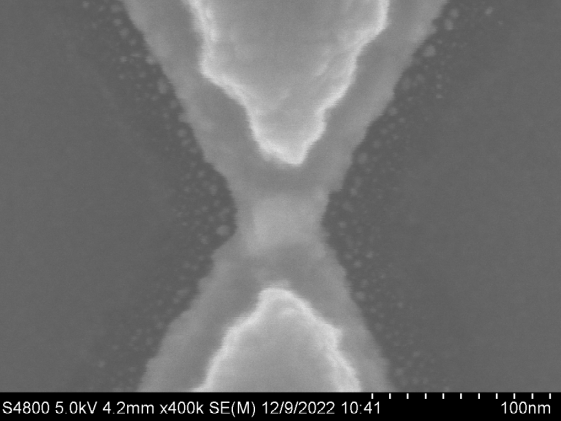
\includegraphics[width=\textwidth]{BeforeMigration.png}
         \caption{SEM image taken of a device before migration. \vspace{1.3cm}}
         \label{fig:BeforeMigration}
     \end{subfigure}
     \hfill
     \begin{subfigure}[b]{0.49\textwidth}
         \centering
         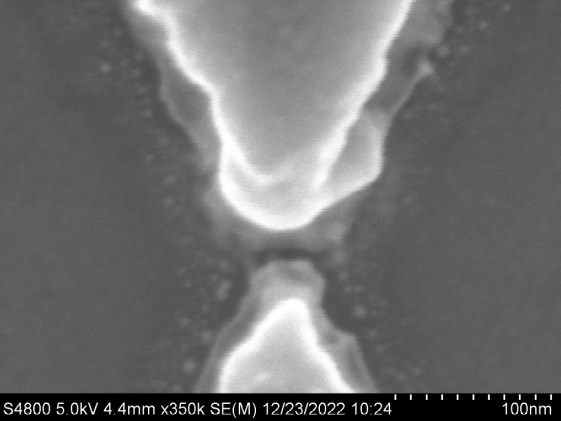
\includegraphics[width=\textwidth]{AfterMigration.png}
         \caption{SEM image taken of a device after migration. It is clear from the picture that material has moved from the bottom to the top in this image, against the direction of the applied bias voltage.}
         \label{fig:AfterMigration}
     \end{subfigure}
        \caption{Two SEM images taken before and after electromigration. The images are taken of different devices created with the same design. In the migration process, the bias voltage was applied from the bottom of the image towards the top. The regions of the device not shown in these images were not visibly changed during the migration process.}
        \label{fig:MigrationBeforeAfter}
        
\end{figure}

Historically, EM was of interest because it caused interconnects in integrated circuits to fail [1]. This was an expensive problem which received a lot of attention from the electronics industry. More recently, however, EM has also been used productively in creating nanoscale gaps in metallic structures. These gaps can have many uses, with the most prominent being single molecule junctions [1]. EM is useful for making single molecule junctions because the size of the gap that is created by EM is of the order of nanometers, the same order of magnitude as many molecules.

\subsubsection{Mechanisms}
The central mechanism driving EM is thermally activated diffusion of the atoms under forces resulting from bias voltage and current [1]. Atoms in the conductor are trapped in a potential well created by neighboring atoms. In order for an atom to escape the potential well, it either needs to be thermally excited such that its energy exceeds the height of the potential barrier, or the barrier must be lowered sufficiently by an applied force. The main forces acting on the atom when a voltage bias is applied to the conductor are the electron wind force, the direct force and the entropic diffusion force. 

When a bias voltage is applied to a conductor, the electrons of the conductor gain a non-zero average momentum. The electrons experience collisions with the atoms, in which momentum is transferred from the electrons to the atoms. When the electrons have non-zero average momentum, the average momentum imparted on the atoms is also non-zero. The electron wind force explains why, when imaging a conductor after EM has taken place, mass can normally be seen to have moved against the direction of the current.  

In a conductor, there are mobile electrons. As a result, the atoms become effectively ionic with a positive charge. When a voltage is applied across the conductor, the ions experience a Coulomb force in the direction of the bias voltage. This is the direct force, and it is directed in the opposite direction from the electron wind force, thus reducing the rate of atomic diffusion [1].

Whenever there exists a spatial concentration gradient, there will be a net movement of atoms in the direction opposite to this gradient, as described by the diffusion equation [1]. The result of this is that atoms located in regions of high atomic density experience a force pushing them in the direction of adjacent regions of lower atomic density. Since EM causes net flow of atoms in one direction, the region that atoms are moved to gets a higher atomic density, while the region that atoms are moved from gets a lower atomic density. This thus results in a concentration gradient pointed in the same direction as the mass flow, and therefore the entropic diffusion force will be pointed in the opposite direction. Entropic diffusion is therefore a stabilizing force which reduces the mass flux. 

Since thermally activated diffusion is the main mechanism behind EM, net mass flux in a conductor is more likely to start in a region of higher temperature. If the conductor has a spatially inhomogeneous thermal conductance coefficient, or experiences inhomogeneous Joule heating, this will cause some regions to become hotter than others, making EM more likely to occur in these regions. There are also regions in the conductor where the potential barrier experienced by the atoms is lower. Atoms on the surface of the conductor, and atoms placed next to grain boundaries, impurities and vacancies, all experience lower potential barriers. These sites are therefore also more likely places for EM to occur.

In order for EM to take place, the current density needs to be sufficiently high. This happens at some critical voltage $V_C$. 

\subsubsection{Effects of Size}
The size of the wire has a significant influence on electromigration. When the wire is of the order of tens of nanometers, as is the case in the devices studied in this thesis, EM tends to progress in a markedly different way as compared to macroscopic wires [1]. In nanoscale wires, the ratio of surface area to volume is orders of magnitude larger than it is, for example, in micron scale wires. In micron scale wires, atomic diffusion happens mainly along grain boundaries. In the smaller nanometric wires, however, diffusion along the surface of the wire dominates. In micron scale wires, macroscopic hillocks and voids tend to form. In nanowires, on the other hand, the wire experiences a gradual narrowing which is localized at the point of highest resistivity. This point experiences the strongest scattering and the highest amount of Joule heating, and therefore it experiences the highest amount of mass flux. The location of this point is dependent on the device geometry and on the microscopic details of the wire, such as the grain boundary structure. 

Studies investigating EM in nanowires have found that it takes place in stages. In the first stage, the wire gradually narrows in one place, with the rest of the wire remaining unchanged. In this stage, Joule heating of the wire causes surface atoms to be promoted to adatoms, which are then swept away against the direction of the current by the electron wind force. When the narrowing progresses to the point that transport becomes quasi-ballistic, the mechanism behind the EM changes. At this point, individual collisions between atoms and electrons are the main driver behind the transfer of mass [1]. 

\subsubsection{Controlling Electromigration}
When using EM to create useful nanogaps, it is important to have a high degree of control over the process. The size of the gap and the resistance of the junction need to be accurately controlled to tailor the junction to its application. When using the junction for single molecule transport measurements, for example, it is necessary that the gap size is similar to the size of the molecule. With regard to achieving this control, there are certain aspects of the device design and the procedure by which the voltage is applied that are particularly relevant. 

When creating a gap in a bridge using EM, the bias voltage will be applied not only over the bridge but also over other resistances between the bridge and the voltage source. The sum of those series resistances is denoted as $R_{S}$, while the resistance of the junction is denoted as $R_{J}$. The junction is the location in the bridge where migration takes place. $R_S$ is for example contributed to by the contact resistance of the voltage source and the resistance of any wires used to connect the voltage source to the junction. When $R_{S}$ is large compared to $R_{J}$, a constant or increasing voltage will cause heating in the junction, which will increase the EM in the junction. This further increases $R_J$, which in turn further increases the EM, in a positive feedback loop that causes a rapid and uncontrolled migration. This leads to an oversized gap and possibly the formation of islands of material inside the gap. In order to avoid this situation, the ratio of series resistance and junction resistance need to be kept in mind when designing the device. This is done for example by connecting the junction to large pads and wires, and making the bridge very thin or giving it a constricted design.

There are multiple ways in which the voltage can be applied to induce EM. Two straightforward ways are to simply ramp up the voltage until the wire breaks, or to apply a constant voltage which is higher than $V_C$ to the junction. These methods offer very little control over the final state of the junction after electromigration. In order to gain more control, the voltage can be applied in pulses. This process is known as pulse EM. Pulse migration adds the parameter of pulse duration, which can increase the level of control the operator has on the EM procedure. The way pulse EM can achieve a desired gap is by repeatedly applying pulses while measuring the resistance of the device. Once this resistance has reached the target resistance, no more pulses are applied. The height and width of the pulses can be changed by the operator based on the increase in resistance each pulse generates. While this method can work in practice [11], the level of control it affords tends to be lower than one can get when using feedback control, which we discuss next.

Feedback controlled EM (FCEM) is a process by which the applied voltage to the device is rapidly changed in response to changes in the resistance of the device [12]. This is done using software that controls the amount of bias voltage applied based on the corresponding amount of bias current. Measuring the current and updating the voltage happens with very high frequency. High frequency is required in order to be able to respond to the changes in the device resistance on an appropriate timescale, on the order of tens of kHz, such that voltage can be ramped back before the resistance has changed too much. The FCEM algorithm operates as follows. A human operator sets the target resistance $R_{Target}$ and the initial voltage $V_i$, and the maximal voltage $V_{max}$. The algorithm now starts to ramp the voltage in small increments from $V_i$ to $V_{max}$. For each applied bias voltage, the current is measured. Using the current, the resistance can be determined using the formula $R = V/I$. For the first few points of the ramp, the calculated resistance values are used to generate an average ramp resistance for the current ramp, $R_{Ramp}$. If, during the ramp, the measured resistance deviates from $R_{Ramp}$ by more than some threshold amount $c \cdot R_{Ramp}$, where $c$ is a parameter specified by the operator which is called the cut-off parameter, then the algorithm brings the current back to $V_i$. If the resistance at this point is still lower than $R_{Target}$, the algorithm starts a new ramp and a new iteration of the algorithm commences. By ramping the voltage back the migration is interrupted before the change in resistance has gotten very large. Because of this, the resistance can only increase in small increments, which allows FCEM to achieve a higher level of control regarding the final resistance. 

The values of the parameters specified by the operator need to be optimized to ensure that EM happens at a sufficient rate while still allowing the algorithm to ramp back fast enough to prevent sudden large changes in resistance [12]. In the first stage of migration, when transport is diffusive, migration happens smoothly and the resistance can be seen to go up gradually. In this stage, the operator should specify a low cutoff parameter. When migration halts or progresses too slowly, $V_{max}$ should be increased. In the second stage, where transport through the junction is ballistic, the migration happens more stochastically and the jumps in resistance are bigger. This stage starts roughly around the 1 k$\Omega$ resistance level, which corresponds to about a dozen atoms in most of the materials commonly used in EM. At this stage, the cut-off parameter should be set high, and the rate of migration controlled using $V_{max}$. The level of control the operator has over the resistance at this stage is lower. Once the resistance reaches a value of around one $R_\textrm{Q}$ = 12.9 k$\Omega$, the junction transitions to the tunnel regime and the level of control drops even further. At this point, the level of resistance reached is only partly controllable by the operator and trial and error on multiple devices may be needed to achieve the desired resistance.
\\

\noindent For certain metals at high enough temperatures, when EM is stopped after increasing the resistance past some threshold value, migration will continue without any applied voltage. This is known as self-breaking. Self breaking happens when atoms rearrange themselves in order to reduce their surface energy. Since the narrowed section of wire created through partial EM has a very large surface area compared to its volume, this is a very unfavored surface-energetic configuration. If the temperature is sufficient and the mobility of the atoms high enough, then the atoms will rearrange themselves in order to reduce their surface energy. In this process, atoms move away from the junction towards the bulk of the bridge. This is a gradual process, and it can be interrupted by cooling down the junction. This means that by stopping EM after the threshold has been reached, and then monitoring the resistance of the junction, the desired resistance can be reached by cooling down the junction once the resistance is close to the target. A benefit of self breaking is that in general the formation of metallic islands in the gap is rare when the gap is created through self breaking.


\subsection{Superconductivity and the Superconducting Proximity Effect}


Superconductivity is a phenomenon first discovered in Leiden in 1911 by Kamerlingh Onnes, when observed that the resistivity of mercury dropped to zero when it was cooled in liquid helium. Superconductivity is characterized by zero resistivity and a complete expulsion of magnetic field. Materials where superconductivity can occur are called superconductors. 

Superconductors are only superconducting when the temperature, current density and applied magnetic field are all low enough [13]. If these quantities become too large, a phase transition occurs and superconductance ceases. Figure \ref{fig:superconducting_phase_transition} shows a typical phase transition surface in temperature-current density-magnetic field space. The maximal temperature at which superconductivity can still occur is known as the critical temperature and is denoted $T_C$. Similarly, the maximal current density and magnetic field where superconductivity can still occur are called the critical current density and critical field, respectively, and are denoted by $J_C$ and $B_C$.

\begin{figure}[H]
     \centering
     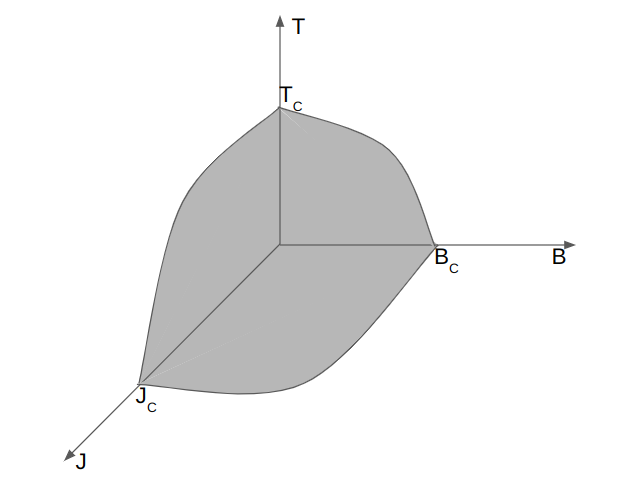
\includegraphics[width=\textwidth]{superconducting_phase_transition.png}
     \caption{A typical superconducting phase transition surface, depicted in gray.}
     \label{fig:superconducting_phase_transition}
        
\end{figure}


\subsubsection{Theoretical Frameworks}

Although superconductivity had been first discovered in 1911, it remained quite poorly understood until the revolutionary work done by Bardeen, Cooper and Schrieffer in 1957. The theory they set forth, the so called Bardeen-Cooper-Schrieffer (BCS) theory, is a microscopic theory that describes superconductivity in terms of phonon-mediated interactions between electrons [12]. In the theory, for superconductors at low enough temperatures, the electron-electron interaction becomes effectively attractive due to electron-phonon interactions. This causes electrons to pair up, forming pairs with opposite momentum and spin called Cooper pairs. The Cooper pairs all occupy the same macroscopic ground state. In the density of states, a gap opens up around the energy of this ground state. This gap is called the superconducting energy gap, and it has a magnitude $|\Delta|$. BCS theory predicts that at zero temperature, the energy gap is proportional to the critical temperature, according to the formula $|\Delta|$ = $1.764 k_BT_C$. \\


Another theory of superconductivity, which preceded BCS theory historically, is the Ginzburg-Landau (GL) theory [13]. GL theory provides a macroscopic, phenomenological description of superconductivity, in terms of a complex order parameter $\Delta$ = $|\Delta|e^{i\phi}$. It turns out that this order parameter is related to the wave function of the Cooper pair wave function. The magnitude of the order parameter is equal to the superconducting energy gap. The characteristic distance over which the order parameter shows significant variation is called the superconducting coherence length, and is denoted $\xi$. GL theory is valid close to $T_C$, when $|\Delta| << k_BT_C$. 

The Gor'kov theory of superconductivity is an extension of BCS theory that gives a description of the superconducting state in the framework of the Green's function formalism [13]. Gor'kov theory is able to predict the behavior of the order parameter and the density of states of the superconductor.

In the limit of $\lambda_F << \xi$, or, equivalently, $|\Delta| << E_F$, which is known as the quasi-classical limit, Gor'kov theory can be simplified. The resulting theory is known as the Eilenberger theory. If, additionally, a system is in the limit of strong disorder, i.e. when the mean free path $l << \xi$, the theory can be further simplified into the Usadel theory. The limit in which the Usadel theory is valid, is known as the "dirty" limit. Many of the results that can be derived using the Usadel theory are used throughout this work.



\iffalse 
Usadel describes superconductivity in terms of the complex functions $F$, which only depend on the so called "Matsubara frequency", $\hbar \omega = \pi k_BT(2n+1)$ and the position $\mathbf{r}$. The Usadel equations can be expressed in an especially simple form by introducing the variable $G = (1-FF^\ast)^{1/2}$. The Usadel equation for $F$ then becomes \cite{Likharev}

$$
2\omega F - D(\nabla - i \frac{2e}{\hbar c} \mathbf{A})\left[G\left(\nabla - i \frac{2e}{\hbar c} \mathbf{A}\right)F - F\nabla G \right] = 2 \hbar^{-1} \Delta G
$$

By summing $F$ with over the Matsubara frequencies, the measurable quantities, i.e. the supercurrent and order parameter, can be derived as follows:

$$
ln(T_C/T) = \Delta ln(T_C/T) = 2\pi k_BT \sum_{\omega > 0} [(\Delta / \hbar \omega) - F]
$$
and
$$
\mathbf{j_s} = \sigma_N(2\pi k_BT/e) \sum_{\omega > 0} Im[F^\ast \left(\nabla - i \frac{2e}{\hbar c} \mathbf{A}\right)F]
$$
\fi



\subsubsection{Proximity Effect and Andreev Reflections}
When a superconductor and a normal metal are brought into contact, there is a transition region in which the order parameter varies between its value deep inside the superconductor, $\Delta_{SC}$, and its value deep in the normal metal, which is 0. In this transition region, the normal metal has a nonzero order parameter and becomes superconducting. This is known as the superconducting proximity effect. The strength of the proximity effect decreases further away from the superconductor-normal metal (SN) interface, and the characteristic length over which this drop-off happens is denoted $\xi_N$, and is of the order of $\sqrt{D/T}$, where $D$ is the diffusion constant in the normal metal. Conversely, the order parameter inside the superconductor is lower closer to the interface with the normal metal than it is far away from this interface. As a result, superconductivity in this region is suppressed. This is called the inverse superconducting proximity effect. The proximity effect can be understood microscopically by examining the transport physics at an SN interface.
 

Charge transport at an SN interface happens in a way that is different from charge transport between two normal metals. If we assume that there is no tunnel barrier between the superconductor and normal metal, transport happens as follows; When an electron passes from the normal metal to the superconductor, and the energy $\varepsilon$ of the electron is higher than $|\Delta|$, the electron can enter the superconductor and occupy a single quasi-particle state. The density of states below $|\Delta|$ is zero, however, and therefore an electron coming from the normal metal with energy $\varepsilon < |\Delta|$ can not enter the superconductor in the normal way. In that case, a hole can be reflected from the SN interface at the same time the electron passes through, and in the process a Cooper pair added to the superconductor. This process is called Andreev reflection. Since a hole has charge e, and a Cooper pair has charge -2e, charge is conserved during Andreev reflection. In order to ensure conservation of energy, the hole needs to have energy -$\varepsilon$. Conversely, when charge is transported from the superconductor to the normal metal, the mechanism is reversed. If the charge crossing the SN barrier is a single quasi-particle with energy $\varepsilon > |\Delta|$ it can pass to the normal metal as it would when passing through a normal metal interface. When a Cooper pair is responsible for the charge transfer, two electrons enter the normal metal with an energy difference of $2\varepsilon$. These electrons still carry their Cooper pair correlation after passing the SN barrier. The characteristic time it takes the electrons to lose this correlation is the dephasing time $\tau = \hbar/\varepsilon$. In this time, the electrons travel a distance $L = \sqrt{D\tau}$ on average in the direction of propagation. As a result, the electrons with energy less than $D\hbar/L^2$ will still carry their Cooper pair correlations at distance L from the SN interface in the direction of propagation. When $L$ is the total length of the normal metal, this energy is called the Thouless energy, and denoted $E_{Th}$.

\begin{equation}
\label{eq:E_Th(D,L)}
E_{Th} = D\hbar/L^2
\end{equation}



 Since the electrons with $\varepsilon > |\Delta|$ are coming from the single particle continuum and did not carry Cooper pair correlation to begin with, those electrons in the normal metal that carry Cooper pair correlations must have energy $\varepsilon < \mathrm{min}\left(E_{Th}, |\Delta|\right)$, and only those electrons contribute to the superconducting transport through the normal metal.


\subsubsection{Superconductivity in SN Bilayers}
In situations where the Usadel theory is valid, the critical temperature of an SN bilayer can be predicted theoretically based on the Usadel formalism, as is done in [15] for example for the case of thin films. In this case, the thin film limit is that limit where the thickness of the superconductor and of the normal metal are small in comparison to their respective superconducting coherence lengths. The formula derived for the critical temperature $T_C$ of an SN bilayer in this limit is given by eq. \ref{eq:BilayerTc}.

\begin{equation}
\label{eq:BilayerTc}
T_C = T_{C0} \left[ \frac{d_s}{d_0} \frac{1}{1.13(1+1/\alpha)} \frac{1}{t} \right] ^\alpha
\end{equation}

\noindent where $$ 1/d_0 = (\pi/2)k_BT_{C0}\lambda_f^2n_s $$ and $$ \alpha = d_nn_n/d_sn_s $$ In these equations, $T_{C0}$ is the critical temperature of the bare superconductor, $d_n$ and $d_s$ are the thicknesses of the normal metal and superconductor, respectively, and $n_n$ and $n_s$ are the respective volumetric electron density of states at the Fermi energy. The parameter $t$ represents the interface transparency. In practice, for most clean metals and interfaces, $t$ tends to be of the order of 0.1 to 1. The interface parameter can be reduced in case of a lattice mismatch, a difference in Fermi velocity, or a contaminated or oxidized contact surface.\\

The devices studied in this thesis contain Pd-Nb and Au-Nb bilayers. Therefore, these materials are of particular interest, and for this reason those material properties that occur in equation \ref{eq:BilayerTc} have been tabulated in table \ref{tab:Bilayer_Table}.

\begin{table}[H]
\centering
\caption{Critical temperature $T_{C0}$ and volumetric electron density of states at the Fermi level $n$ for relevant materials.}
\label{tab:Bilayer_Table}
\begin{tabular}{|c|c|c|}

\hline 
Metal & $T_{C0}$ (K) & $n$ (states / eVcm$^3$) \\ 
\hline 
Nb, 100 nm & 9.1  & 5.07 $\cdot$ 10 $^{22}$ \\ 
\hline 
Nb, 50 nm & 8.9 & 5.07 $\cdot$ 10 $^{22}$ \\ 
\hline 
Ti & 0.49  & 2.93 $\cdot$ 10 $^{22}$ \\ 
\hline 
Pd & - & 1.55 $\cdot$ 10 $^{23}$ \\ 
\hline 
Au & - & 1.60 $\cdot$ 10 $^{22}$ \\ 
\hline 
\end{tabular} 
\end{table}

Once the value of $T_C$ is known, the energy gap of the bilayer can be calculated simply using $\Delta = 1.764 k_BT_C$ in the case of a BCS superconductor.



\subsubsection{Charge Transport in Weak Links}

In the literature on superconductivity, the term "weak link" refers to any structure that connects two bulk superconducting electrodes, for which the critical current is much less than the critical current of the electrodes. All the devices studied in this thesis have this structure, and the theory of weak links is therefore of particular interest.\\


There are several parameters which characterize a weak link. The distance between the superconducting electrodes is referred to as the length $L$ of the weak link. There is another length scale that plays a more central role in weak link transport, however, and that is the effective length $L_\mathrm{eff} \geq L$. The effective length is the length scale over which nonlinear effects are localized. In general, the nonlinear effects are localized over shorter distances in weak links with lower conductivity. Weak links for which the superconducting coherence length $\xi$ is much greater than $L_\mathrm{eff}$ are classified as short junctions, and those for which $\xi \lesssim L_\mathrm{eff}$ are classified as long junctions. 

Within the short junction limit, there is a second classification which is based on the electron mean free path $l$. Weak links for which the effective length is much greater than $l$ are classified as "dirty", and those in the opposite limit are classified as "clean". Usually, electrons in a weak link experience diffusive scattering on the film surface, and as a result $l$ tends to be of the order of the film thickness which is much less than $L_\mathrm{eff}$. 


The devices studied in this thesis have bridge thickness that is much smaller than the bridge length and therefore also much smaller than the effective length, and they can thus be classified as dirty weak links.


\subsubsection{Josephson Junctions and the $I_CR_N$ Product}

The critical $I_C$ is defined as the maximal equilibrium supercurrent of a system [14]. When the current crosses $I_C$, there is a jump in the resistance of the system. The magnitude of this jump is the normal resistance $R_N$. Together, the critical current and normal resistance define a voltage, the critical voltage $V_C = I_CR_N$. The critical voltage is an important parameter in the description of many superconducting systems.

In the case of superconductor-insulator-superconductor (S-I-S) junctions, the critical voltage is proportional to the energy gap:

$$
I_CR_C = \pi \Delta/ 2e
$$


For the special case of dirty S-N-S junctions, the Usadel equations can be solved to find the relationship between $V_C$ and temperature for various ratios of $L$ and $\xi_N$ at the critical temperature of the superconductor. This relationship is captured in the graph in figure \ref{fig:V_C_of_T_for_different_L_over_Xi}, which has been reproduced from [13] with slight modifications. 

\begin{figure}[H]
     \centering
     \hspace{0.7cm}
     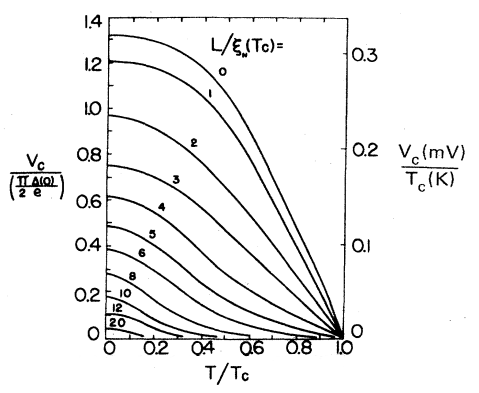
\includegraphics[width=0.5\textwidth]{Likharev_Graph.png}
     \caption{This figure has been reproduced with modifications from [13]. Theoretical predictions of the critical voltage $V_C$ as a function of temperature, for different values of $L/\xi_N(T_C)$.}
     \label{fig:V_C_of_T_for_different_L_over_Xi}
        
\end{figure}

In this limit, the Usadel equations also allow for the derivation of formula \ref{eq:Xi_N_of_T}. In this formula, $D$ is the diffusion coefficient in the normal metal. 


\begin{equation}
\label{eq:Xi_N_of_T}
\xi_N(T) = \sqrt{\frac{\hbar D}{2\pi k_BT}}
\end{equation}







\iffalse
In long junctions in the dirty limit, the Thouless energy and $I_CR_N$ are found to be proportional at zero temperature:

\begin{equation}
\label{eq:IcRn_at_low_T}
eI_CR_N = \pi E_{Th} 
\end{equation}


This equation can be extended using quasiclassical theory when $E_{Th} << \Delta$, and the extended relationship is given in equation \ref{eq:generalized_thouless_energy}.

\begin{equation}
\label{eq:generalized_thouless_energy}
eI_CR_N \approx \frac{32}{3+2\sqrt{2}} E_{Th} \left[ \frac{2\pi T}{E_{Th}} \right]^{\frac{3}{2}}e^{-\sqrt{\frac{2\pi T}{E_{Th}}}}
\end{equation}


Get the following formula in somewhere :

$$
D = v_f l/3
$$


Length and effective length, Long and Short junction limit, Dirty vs Clean limit of junction (n.b. not of superconductor)


Gindsberg landau assumptions + formulas

Formula 41 on IcRn product and $\Delta_{1/2}$

Usadel equations assumptions + formulas

Formula 76, 78 on IcRn

Formula 142 maybe?

\fi






\newpage
\section{Methods}
\label{section:Methods}

\subsection{Fabrication}


\subsubsection{Electron Beam Lithography}
Fabrication of the junctions was done using electron beam lithography. This process is depicted schematically in figure \ref{fig:EBL}.
In this process, one starts with the substrate on which the device will be fabricated. The substrate used for all devices discussed in this thesis was p+ doped silicon covered by silicon oxide. The p+ doped silicon conducts electricity, while the silicon oxide is a dielectric. This means that the substrate can be used as a global back gate. This substrate is next cleaned using red fuming nitric acid.

\begin{figure}[H]
     \centering
     \begin{subfigure}[b]{0.49\textwidth}
         \centering
         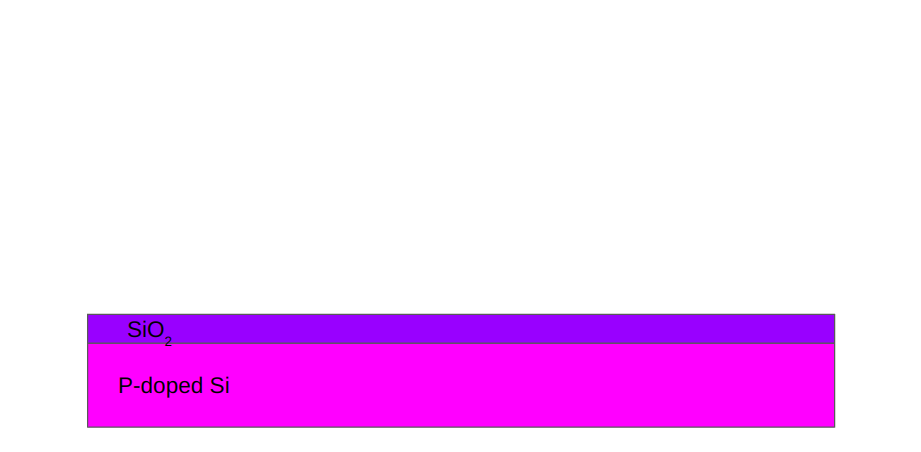
\includegraphics[width=\textwidth]{EBL1.png}
         \caption{A cleaned substrate.\newline}
         \label{subfig:EBL-a}
     \end{subfigure}
     \hfill
     \begin{subfigure}[b]{0.49\textwidth}
         \centering
         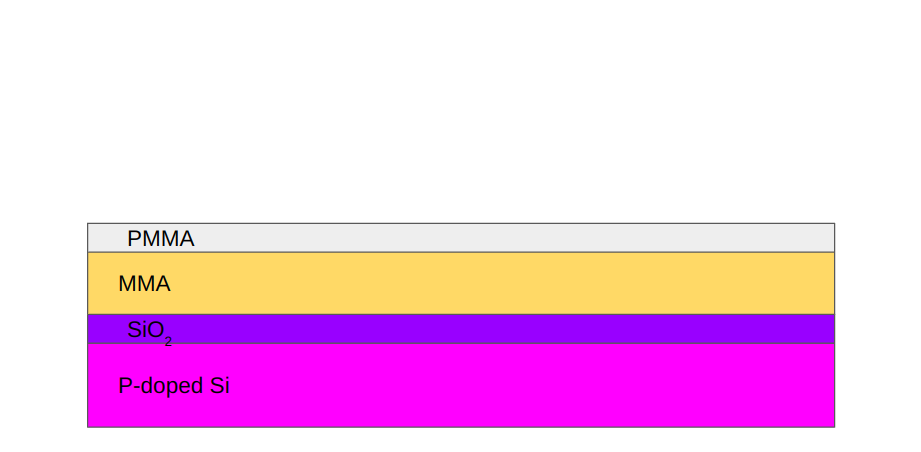
\includegraphics[width=\textwidth]{EBL2.png}
         \caption{Layers of PMMA and MMA are added onto the resist by spin-coating.}
         \label{subfig:EBL-b}
     \end{subfigure}
     \hfill
     \begin{subfigure}[b]{0.49\textwidth}
         \centering
         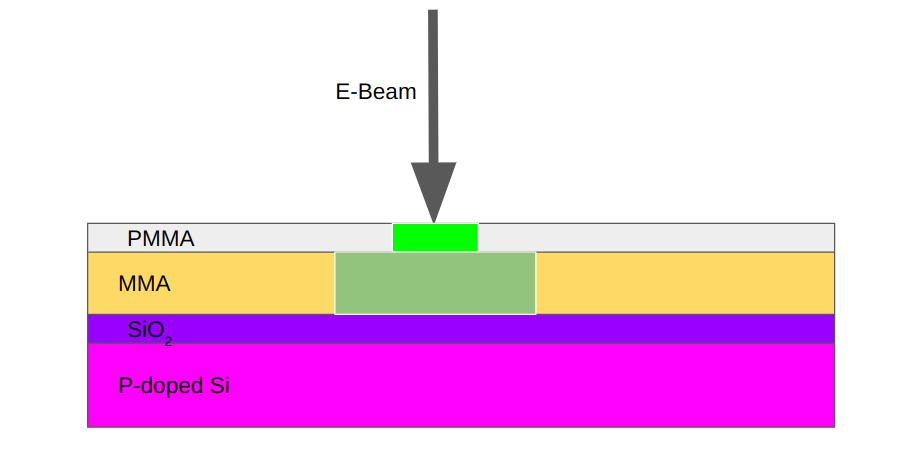
\includegraphics[width=\textwidth]{EBL3.png}
         \caption{A portion of the resist is irradiated with an electron beam in a specified pattern.}
         \label{subfig:EBL-c}
     \end{subfigure}
     \hfill
     \begin{subfigure}[b]{0.49\textwidth}
         \centering
         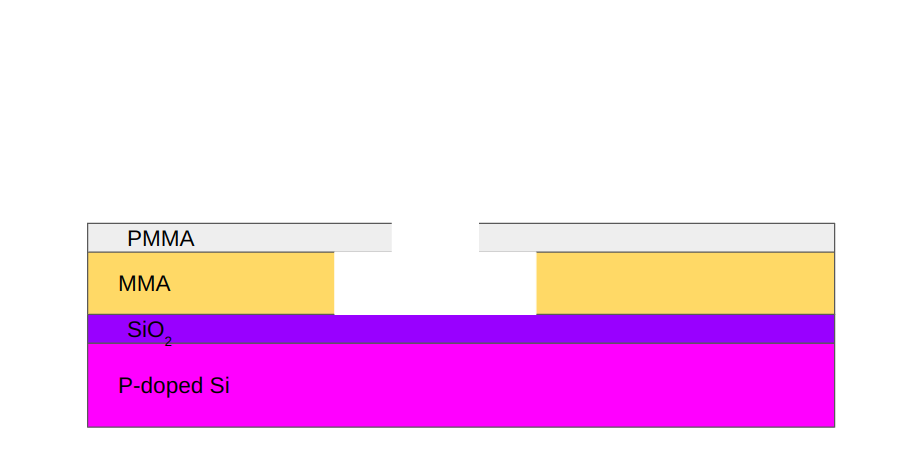
\includegraphics[width=\textwidth]{EBL4.png}
         \caption{The irradiated region is dissolved away. \newline}
         \label{subfig:EBL-d}
     \end{subfigure}
     \hfill
     \begin{subfigure}[b]{0.49\textwidth}
         \centering
         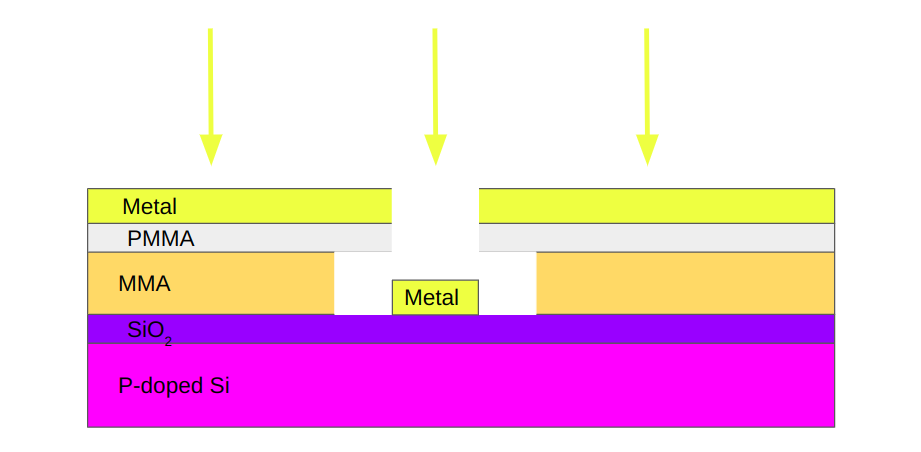
\includegraphics[width=\textwidth]{EBL5.png}
         \caption{Material is evaporated onto the mask and substrate.}
         \label{subfig:EBL-e}
     \end{subfigure}
     \hfill
     \begin{subfigure}[b]{0.49\textwidth}
         \centering
         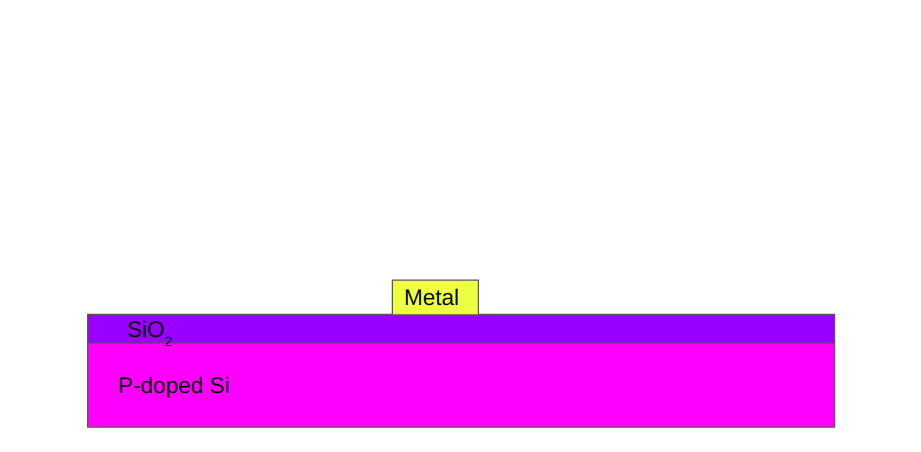
\includegraphics[width=\textwidth]{EBL6.png}
         \caption{The mask is removed, leaving the patterned material on the substrate.}
         \label{subfig:EBL-f}
     \end{subfigure}
        \caption{Electron Beam Lithography Process Diagram.}
        \label{fig:EBL}
        
\end{figure}

The cleaned substrate is covered by a layer of the resist methyl methacrylate (MMA),  which is dissolved in ethyl lactate at 8\% concentration, using a technique known as spin-coating. This technique allows for a very thin film of MMA to be deposited, with a high level of control on the final thickness. The MMA was spin coated at 2000 rpm for one minute and next baked for 5 minutes at 180 $^{\circ}$C to remove the solvent and fix the resist. This recipe creates an MMA layer of 340 nm thick. On top of this layer, 80 nanometers of poly methyl methacrylate (PMMA) with a molecular weight of 950K, dissolved in anisole at 2\% concentration, is deposited by spin coating for 60 seconds at 2000 rpm, which is also followed by a 5-minute bake at 180 $^{\circ}$C, which creates a layer of PMMA of 80 nm thick (Figure \ref{subfig:EBL-b}).

PMMA and MMA are both sensitive to electron bombardment. When these resists are irradiated with electrons, polymeric chains are broken and as a result the solubility is increased (Figure \ref{subfig:EBL-c}, color change reflects change in solubility). An electron beam lithography machine is able to expose the resist in a specified pattern with a resolution of close to 1 nm. Due to the additional exposure of the resist by indirect, scattered electrons, the maximal resolution is reduced to the order of 10 nanometers. Due to the lower molecular weight of the MMA compared to the PMMA, the MMA needs less exposure to become soluble. This causes a larger region of MMA to be effectively irradiated.

After exposure with the electron beam, the sample is developed by submersing it in a 3 to 1 mixture of isopropyl alcohol (IPA) to methyl isobutyl ketone (MIBK) for 90 seconds. This causes the exposed area of the resist to dissolve and be removed, while the less soluble unexposed resist remains (Figure \ref{subfig:EBL-d}). Since a larger area of PMMA was effectively exposed compared to the MMA, there is a region where the PMMA gets removed while the apposed MMA remains. This region of the PMMA is called the undercut, while the region of MMA that hangs above the undercut is called an overhang. The sample is next transferred to pure IPA to stop the development process. After development, the sample is exposed to oxygen plasma for 20 seconds. This is a cleaning step that removes unwanted residues that may have been left after the development.

Next, the mask that was created in the preceding steps is ready for metallization. It is placed in an evaporation chamber, and metal is deposited using electron beam evaporation. This results in a thin layer of metal being deposited on the sample, as shown in figure \ref{subfig:EBL-e}. Many metals do not stick to the SiO$_2$ layer reliably, and as a result they may come off during further fabrication steps. To remedy this, often a different layer of metal is deposited on the SiO$_2$ first. Such a layer is known as a sticking layer, and all devices discussed in this thesis have been made using a 5 nm titanium sticking layer.

Finally, the mask and the portion of the metals that was deposited on top of the mask is removed, in a process known as lift-off. This is done by submersing the sample in N-Methyl-2-pyrrolidone (NMP), heated to 80 $^{\circ}$C for multiple hours. This dissolves the resist and thereby also removes the metal that was supported by that resist, as shown schematically in figure \ref{subfig:EBL-f}.

\subsubsection{Double Angle Evaporation}
In the preceding subsection an outline of the EBL process was described. If one wants to design a device with multiple layers of metal, where each metal is deposited in a different shape, the entire EBL process can be repeated. The resist is applied on top of the substrate and the already deposited metal, and irradiated according to a new pattern. After development this will form a new mask such that a new layer of metal can be evaporated onto the substrate in a different pattern. A notable difficulty with this method of producing different patterned layers is that the patterns of the different layers need to be properly aligned. This alignment happens with finite accuracy, and therefore can introduce imperfections in the device geometry. Another drawback is that it is more arduous to go through all the EBL steps a second time than it would be to reuse the same mask for multiple layers. 

\begin{figure}[H]
     
     \begin{subfigure}[b]{0.49\textwidth}
         \centering
         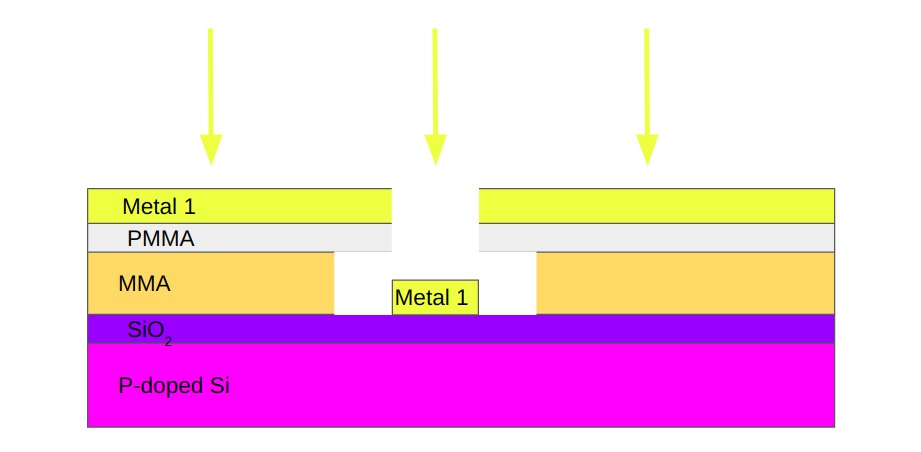
\includegraphics[width=\textwidth]{DoubleAngle1.png}
         \caption{The first layer of material is evaporated onto the mask and substrate. \newline}
         \label{subfig:evaporation-first}
     \end{subfigure}
     \hfill
     \begin{subfigure}[b]{0.49\textwidth}
         \centering
         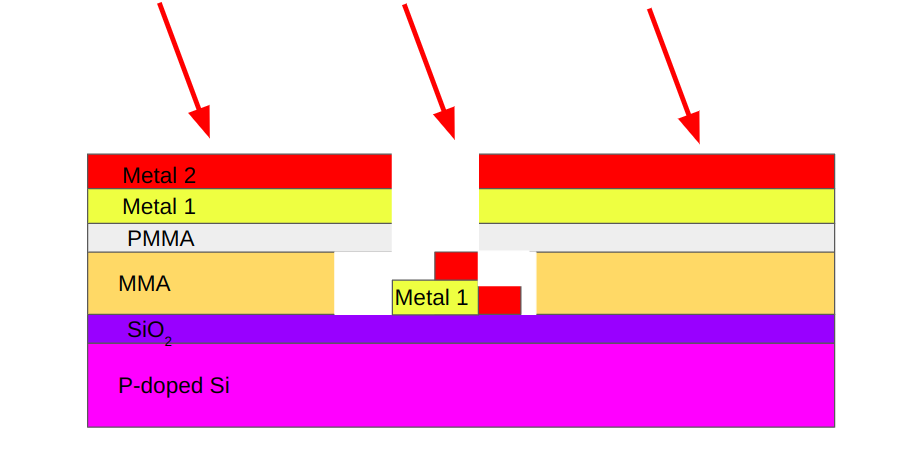
\includegraphics[width=\textwidth]{DoubleAngle2.png}
         \caption{The second layer is evaporated at a different angle, causing a translation with respect to the first layer.}
         \label{subfig:evaporation-second}
     \end{subfigure}
        \caption{Double angle evaporation.}
        \label{fig:DoubleAngle}
        
\end{figure}

There is another way of creating a device with multiple differently patterned shapes that only involves the use of a single mask. This process is known as double angle evaporation. As the name suggests, double angle evaporation involves evaporating the different layers of metal at different angles. Since the mask has a nonzero thickness, the different angles result in a relative translation between the different evaporated layers. Evaporating the material at an angle with respect to the normal of the substrate also causes a stretching of the masked pattern. Because the same mask is used for different layers of material, these layers are automatically well aligned. There are some drawbacks to this method. One drawback is that the different layers need to be translated copies of each other, making this technique only useful in cases where this class of patterns is sufficient for the device being fabricated. Another drawback is that whenever material is evaporated at an angle to the normal, there needs to be enough undercut to accommodate the translated pattern. When undercuts get too big, the corresponding overhangs can become unstable and the mask may fail. 

\subsubsection{Design}

Most often, when contacting nanoscopic objects using EMBJs, the bridge material of choice is gold. Gold atoms have a relatively high mobility, which makes electromigrating gold easier and allows for self breaking at room temperature. Gold is also highly unreactive, such that the quality of the contacts is not degraded by oxidation as it would be with a more reactive material. Another reason to choose gold is that it has a relatively high electrical conductance. The most obvious drawback, however, is that not all objects can be optimally contacted with gold. Some objects, such as GNRs, have a work function that does not match as well with the work function of gold as with some other metals, which can result in Schottky barriers or poor band alignment. For those objects, a different bridge material needs to be chosen. Palladium has been found to have a work function that is well suited for contacting GNRs [9], and even more so for contacting carbon nanotubes. Palladium atoms are less mobile than those of gold, which means that migration may require larger temperatures or currents, and that self-breaking at room temperature does not typically take place, or takes place only over much larger time scales. Palladium is also slightly more reactive than gold. For many objects that are hard to contact with gold, and GNRs specifically, palladium is a good choice for the bridge material. This is why palladium was chosen as the bridge material to be studied in this thesis.\\


\noindent Since the goal is to create superconducting EMBJs, and since palladium does not by itself become superconducting at low temperatures, superconductivity needs to be induced in the palladium using the proximity effect. 

From our discussion on the proximity effect in the chapter on Theory, specifically equation \ref{eq:BilayerTc}, we conclude that the best way to induce superconductivity in the palladium is by having a thin palladium layer covered by a thick layer of superconductor, at least in the limit where both films are much smaller than their respective coherence length. The superconductor should have a high $T_C$ and a high DOS at the Fermi energy. Niobium was chosen in the designs studied in this thesis, since out of the available superconductors it has a good combination of a high $T_C$ with a relatively high DOS at the Fermi level. The fact that niobium can be evaporated means that double angle evaporation is possible, since the deposition is unidirectional when depositing using evaporation. When depositing material using sputtering, however, deposition happens in all directions making double angle evaporation impossible. As mentioned, using double angle evaporation makes the fabrication process significantly easy and less susceptible to error by eliminating the need for multiple cycles of spin coating, e-beam and development, and the need to align successive patterns.\\


\noindent Having selected palladium for the bridge material and niobium for the proximitizing superconductor, and single step double angle evaporation for the fabrication, we need to determine the geometry of the devices. The main geometric choices to be made are the respective thicknesses of the palladium and niobium, the distance between the niobium and the center of the bridge and the constriction geometry.

For the constriction geometry, the main design goals are to reliably have electromigration create the gap in the center of the bridge, and to have a high electronic diffusion coefficient throughout the bridge, since that implies a higher Thouless energy

When electromigration consistently happens near the center of the bridge, the chance that other materials than the bridge material, such as the titanium sticking layer or the niobium layer, diffuse into the leads during electromigration. Such a mixing of different kinds of atoms leads to reduced diffusion and thereby reduced superconductivity, and it leads to an uncontrolled and undesired contact surface. Consistency in breaking is furthermore desirable since a variable gap location, which leads to variable superconducting properties, adds an uncontrolled variable to transport measurements done using the EMBJ and reduces interpretability and reproducibility of the results. Electromigration is most likely to start in areas of high local resistance, and is especially likely to start at grain boundaries. Since the local resistance of the bridge is inversely proportional to the local cross-sectional area, a sharp constriction where the cross-sectional area is much smaller in the center than in the rest of the bridge will most reliably break close to the center. 

Since the Thouless energy is proportional to the electronic diffusion coefficient in the bridge, we want to choose a geometry in which this coefficient is high. The electronic diffusion coefficient is proportional to the electron mean free path. In thin films, such as our bridge, the effect of edge scattering on the mean free path is significant. In a very constricted geometry, the mean free path becomes very small near the constriction due to edge scattering, and diffusion becomes poor. 

\begin{figure}[H]
     
     \begin{subfigure}[b]{0.49\textwidth}
         \centering
         
\includegraphics[width=\textwidth]{restriction_tight.png}
         \caption{A sharp constriction, with good gap localization but poor diffusion.}
         \label{subfig:constriction-sharp}
     \end{subfigure}
     \hfill
     \begin{subfigure}[b]{0.49\textwidth}
         \centering
         
\includegraphics[width=\textwidth]{restriction_loose.png}
         \caption{A blunt constriction, with good diffusion but poor gap localization.}
         \label{subfig:constriction-blunt}
     \end{subfigure}
        \caption{A comparison of restriction geometries.}
        \label{fig:ConstrictionGeometries}
        
\end{figure}

In our design, a bowtie geometry with a 60$^\circ$ constriction angle was chosen because it was hypothesized to be a good compromise between having good diffusion and good gap localization.\\


\noindent The choice of palladium thickness is motivated by our desire to have good induced superconductivity and good electromigration.

In order to have good electromigration, the bridge resistance should be high compared to the series resistance. Since the bridge resistance is smaller for thicker bridges, the bridge thickness should not be so big that electromigration becomes difficult. 

In order to have good superconductivity, there are two competing considerations. Equation \ref{eq:BilayerTc} tells us that the palladium will have a higher induced $T_C$ when it is thinner compared to the niobium, at least in the thin film limit. A thicker palladium layer also causes more inverse proximity effect in the niobium, thereby increasing the effective distance from the niobium to the gap. It also reduces the energy gap in the bilayer.

The mean free path of the leads, on the other hand, is inversely proportional to the resistivity of the film, which increases with thinner films. This therefore leads to a reduced Thouless energy. 

Based on these considerations, a palladium thickness was chosen to be 13 nm in the bridge.\\

\noindent Based on the theoretical discussion of the proximity effect, we concluded that a thicker layer of superconductor implies a better proximity effect, where the proximity effect starts to saturate asymptotically as the thickness of the superconductor becomes much larger than the coherence length of the superconductor. Therefore, we wish to make the niobium layer as thick as possible within the constraints of the fabrication process. 

Niobium has a very high evaporation temperature. Consequently, the substrate on which the niobium is deposited is heated substantially during the deposition. When more niobium is deposited, more heating takes place and more film stress can develop. This can damage the resist layer and lead to fabrication defects. Thinner layers tend to have a cleaner fabrication with fewer defects. 

Based on these considerations, our initial guess for the ideal thickness of the niobium layer was 100 nm.\\


\noindent The degree of proximitization of the normal metal decreases as the distance to the superconductor increases. In order for the leads to be optimally proximitized the niobium should be deposited as close to the center of the bridge as possible without any niobium ending up at the site where the break is created during electromigration. When using shadow mask evaporation, there is always a region around the pattern where small amounts of material inadvertently end up. If the niobium layer is patterned too close to the center of the bridge, this will lead to unintended niobium deposition onto the leads. This constrains the distance between the niobium deposition region and the center of the bridge. In our design, we chose this distance to be 25 nm. \\


\noindent As mentioned in the section on EBL, a 5 nm titanium sticking layer is used to ensure that the other layers stick to the substrate. The sticking layer is evaporated at a right angle to the substrate, such that it does not end up underneath the bridge. Since the bridge has only a small contact area with the surface, its connection to the rest of the device is sufficiently strong to hold it in place and no sticking layer is needed there. The absence of titanium under the bridge reduces the likelihood of a palladium titanium alloy forming during the migration process. This increases the probability that the resulting contacts are made of pure palladium as intended. The absence of titanium under the bridge also improves the superconductivity of the bridge, since titanium is a normal metal above 0.49 K and would inversely proximitize the bridge in that temperature range. The final device design is depicted in figure \ref{fig:device_design}.

\begin{figure}[H]
     \centering
     \begin{subfigure}{\textwidth}
         \centering
         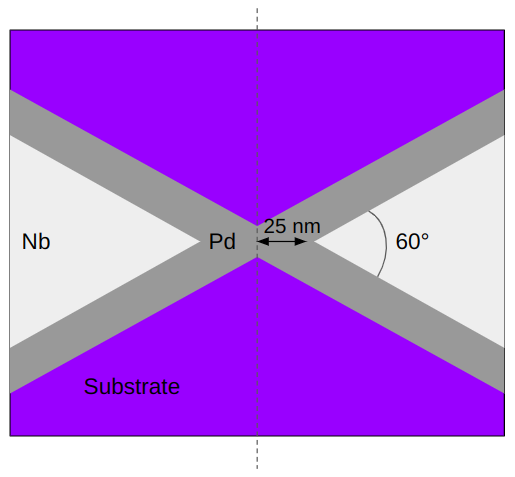
\includegraphics[width=0.6\textwidth]{layout_top.png}
         \caption{Device design, top view. The titanium sticking layer is located underneath the palladium, in the same pattern as the niobium.}
         %\label{}
     \end{subfigure}
     \newline
     \begin{subfigure}{\textwidth}
         \centering
         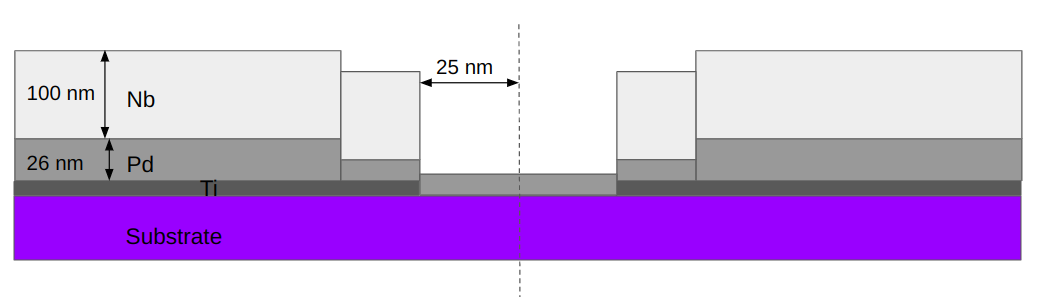
\includegraphics[width=\textwidth]{Layout_Side_2.png}
         \caption{Device design, side view.}
         %\label{}
     \end{subfigure}
        \caption{Device design.}
        \label{fig:device_design}
        
\end{figure}

\subsubsection{Further Design Iterations}
During this thesis, the initial design outlined in the previous section was iteratively changed a total of three times. The goal in each design iteration was to improve the electromigration and superconducting qualities of the device. The changes that were made were in each iteration were based on the information gained from the results of transport measurements that were done on the devices of the previous iteration. In some cases the changes were also based on the results of fabrication tests. Devices made with the initial design are referred to in this thesis as PdNb devices.  

The first change that was made was the substitution of gold for palladium as the bridge material. This change was made because no superconductivity was measured in the PdNb devices after electromigration. Since gold has a density of states at the Fermi energy that is approximately an order of magnitude lower than that of palladium, this substitution was hypothesized to increase the degree to which the bridge material was proximitized. Devices made with this second design are referred to in this thesis as AuNb devices, or sometimes AuNb devices with 100 nm niobium thickness.

In the second design iteration the thickness of the niobium layer was reduced from 100 nm to 50 nm, and the thickness of the gold layer was increased from 13 nm in the bridge to 15 nm. The rate at which the niobium was evaporated was also increased, from 0.2 nm/s to 0.5 nm/s. The reason for decreasing the thickness of the niobium layer and increasing its evaporation rate was that SEM images of the devices with the previous design showed that the niobium layer was not shaped as intended, while niobium layers evaporated with the new parameters were shown to be as intended in a fabrication test. The motivation for increasing the gold thickness was that a thicker layer of gold has a larger conductance and therefore a larger mean free electron path and a higher electronic diffusion constant, which leads to better proximitization of the bridge and an increase in the Thouless energy. The downsides of a thicker layer of gold is a lower bilayer $T_C$, and a lower bridge resistance, which is disadvantageous to electromigration. Despite this trade-off, it was hypothesized that a thicker gold layer would improve device quality. The devices made with this design are referred to in this thesis as AuNb devices with 50 nm Nb.

The final design change was an increase in the bridge length from 50 nm to 60 nm. It was hypothesized that this change would lead to more consistent gap formation during electromigration. Devices with this design are referred to in this thesis as AuNb devices with 60 nm bridge spacing. 

\subsubsection{Chip Preparation}

Devices were typically fabricated on a 19 mm by 19 mm substrate, with a layout as shown in figure \ref{fig:device_layout}. On this substrate, a grid of 9 sets of devices was usually fabricated, where each set contains 5 rows of 8 devices.

\begin{figure}[H]
     \centering
     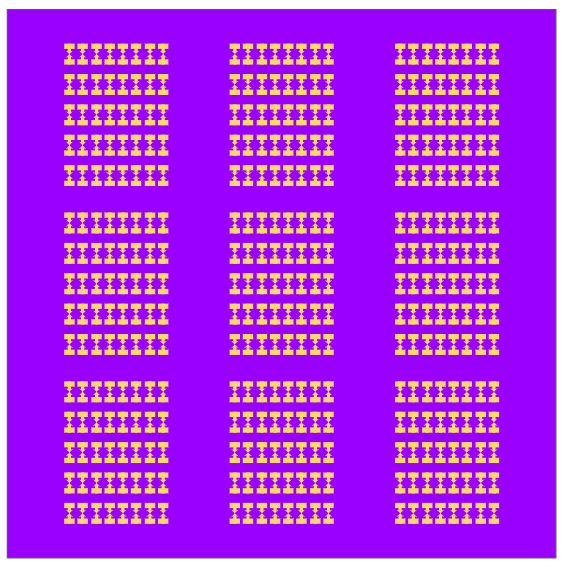
\includegraphics[width=0.6\textwidth]{device_layout.png}
     \caption{A schematic representation of the final device layout on the substrate.}
     \label{fig:device_layout}
        
\end{figure}

In order to be able to load the devices into the measurement set-up, they need to be put on a chip carrier. Because of the size of the chip carrier, the 19 mm by 19 mm substrate needs to be cut into 9 separate pieces, each containing a single set of devices. One such set then fits on the chip carrier. The substrate was first scratched using a diamond tipped scratcher along a crystallographic direction and then broken along this scratch by applying a bending force to the substrate using breaking pliers. The set of devices thus obtained is then attached to the chip carrier using either silver paste or two-sided carbon tape. Both silver paste and carbon tape are electrically conducting, which creates an electrical connection between the backplate of the chip carrier and the doped silicon of the substrate. Finally, the devices are connected to the chip carrier. The chip carrier contains pads made for electrical connections, and each device has two bonding pads for the same reason. Using a device called a wirebonder, small aluminium wires can be made between the pads of the chip carrier and the bonding pads of the devices. One connection is made between a pad of the carrier and the backplate of the carrier. This pad will allow a gate voltage to be applied to the devices. At this point, the device is ready to be loaded into the measurement set-up. The chip carrier containing a chip and wirebonds, connected to the backplate via silver paste, is shown in figure \ref{fig:chip_carrier}.

\begin{figure}[H]
     \centering
     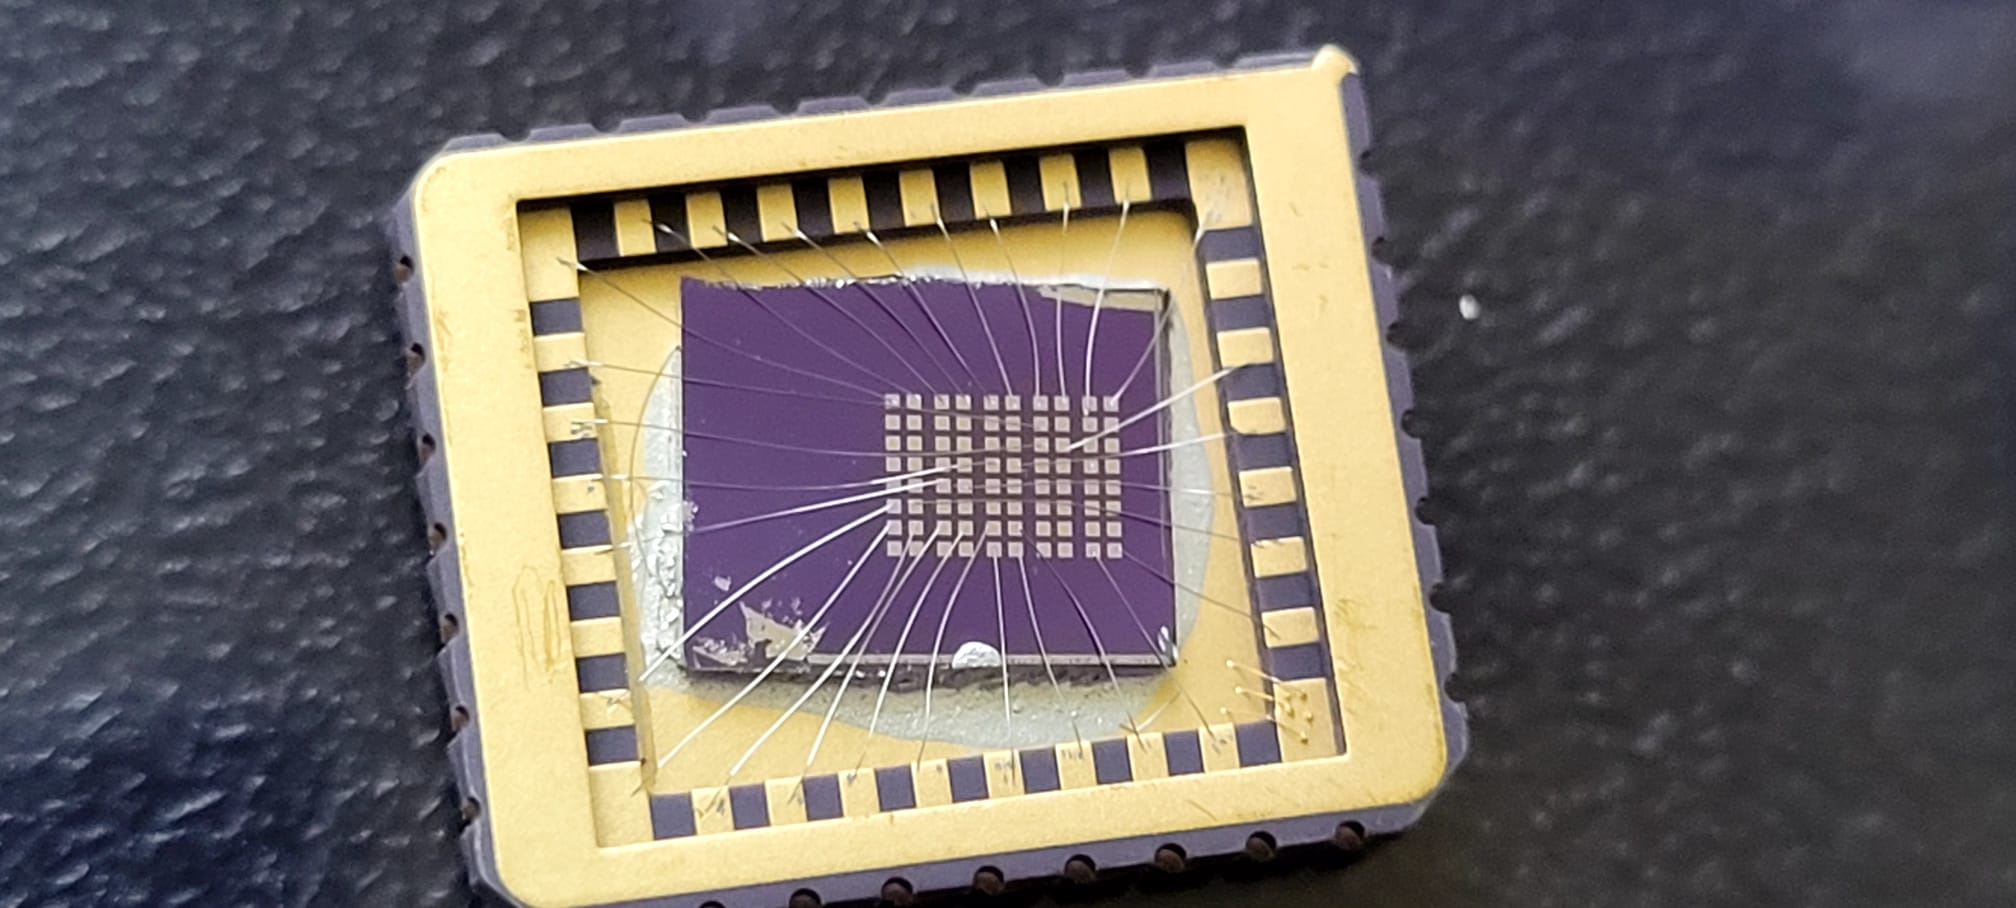
\includegraphics[width=\textwidth]{chip_carrier.jpeg}
     \caption{A chip carrier containing a substrate with a single set of devices. The substrate is connected to the backplate via silver paste. The bonding pads of the devices are connected to the pads of the chip carrier via aluminium wire bonds. A single pad of the chip carrier is connected via wirebonds to the backplate (bottom right).}
     \label{fig:chip_carrier}
        
\end{figure}


\subsection{Transport Measurements}
\label{subsection:transport_measurements}

Since the devices have been designed to break as a result of an applied voltage, electrostatic discharge (ESD), which can supply a sudden pulse of hundreds of volts, can easily destroy a device. Because of this, care needs to be taken to ensure that the devices are protected from ESD. The way this is done is by always wearing a grounding bracelet while touching any modules that are connected to the device, and keeping the devices themselves grounded while measurements are not being performed on them.\\

In order to reach the temperatures needed to observe the superconducting effects of interest at high enough resolution, two cooling setups were used. Both involve the use of liquid helium. Liquid helium has a boiling point of around 4.2 K at atmospheric pressure. 

In the first setup, the sample is loaded into a stick, the so-called dip stick. The interior of the stick contains an inner vacuum chamber where the sample is placed, which is separated from the outside, and a second smaller chamber called the 1K pot, which is connected to the outside of the stick by a small opening which can be opened or (partially) covered using a valve by the operator. The sample makes thermal contact with the 1K pot. The pressure in the main chamber and in the 1K pot can be controlled by attaching pumps to the stick. This stick is submerged in a dewar of liquid helium. By creating a small opening between the 1K pot and the liquid helium while pumping the 1K pot, helium is let into the 1K pot but the pressure inside will be lower than atmospheric pressure. This results in a lowered boiling for the helium and reduces the sample temperature, theoretically as low as 1 K but in practice in this set-up a minimal temperature of 1.6 K was more typically reached. The dipstick set-up contains a heater which allows the temperature to be raised and temperature dependent measurements to be performed. The dipstick set-up contains no magnet and thus no magnetic field dependence can be measured.

The second measurement set up involves a dilution fridge. The dilution fridge is a machine that uses the mixing of two helium isotopes, He$^3$ and He$^4$, to reach temperatures as low as 25 mK. The dilution fridge also contains a vector magnet, which allows the operator to apply a magnetic field in any direction. The magnetic field has a maximum magnitude which depends on direction. In the direction perpendicular to the chip, which we will henceforth refer to as the Z direction, the magnetic field can go as high as 10 T. In the two perpendicular directions which are in plane with the chip, referred to as the X and Y directions, the magnetic field can reach 1 T and 3 T respectively. The presence of the vector magnet allows for measurements with magnetic field dependence in this set-up, and the lower temperatures that can be reached allow for higher resolution measurements.\\

In each of the measurement setups, there is a holder that the chip carrier can be loaded into. This holder contains pins that connect the pads of the chip carrier to a different set of pins which allow the operator to connect to the devices during the measurements. The module containing these pins is called the matrix module, and the rack that this module and the other modules used during a measurement are placed in is called the IVVI-rack. By connecting modules that apply or measure current or voltage to the pins of the matrix module, the operator can perform transport measurements. \\

When doing a transport measurement, care needs to be taken with the choice of measurement to ensure that the measurement is of high quality. In order to ensure this, the operator must choose modules that optimize the input impedance of the measurement modules and the output impedance of the source modules, as well as the amount of noise that results in the measurement. Series resistance and noise lower the quality of the measurement because they result in systematic and random error, respectively. Since the setup is controlled digitally, care must be taken to minimize the influence of the finite precision digital values sent to the IVVI rack.\\

\subsubsection{VI}
One of the most elementary measurements is one where a current source applies a bias current to the device, and voltage is measured over the device. I will refer to this kind of measurement as a VI measurement. With such a measurement, the instructions on what bias to apply are sent to the IVVI rack from the computer. The IVVI rack converts this digital signal to an analog one using a digital to analog converter (DAC). This results in a voltage of between -1.5 V and 1.5 V that is supplied to the current source module. The current source module has a built-in amplifier with multiple possible configurations ranging from 1 nA/V to 10 mA/V, which determines the amount of current it delivers per unit of voltage supplied by the DAC. The amplification setting also determines the output resistance of the module. The output resistance is one over the amplification, such that at 1 nA/V the output impedance is 1 G$\Omega$ and at 1 mA/V it is 1 k$\Omega$, for example. The current is biased over a device, using the appropriate pins from the matrix module. The voltage measurement module is applied in parallel over the same device. This creates a quasi 4 point measurement. The voltage measurement module has an amplifier that can be set to an amplification ranging from 1 to 10k. This module also has a maximal output voltage of 1.5 V. The output of the voltage measurement module goes to a Keithley-2100 digital multimeter, and the value that is measured there is stored on the computer. In order to minimize the digitization error introduced by the limited digital precision, the maximal range of the DAC should be used. For a current source, higher output resistance improves measurement accuracy and therefore the lowest possible amplification should be used. The largest possible amplification should be applied on the voltage measure module that allows it to stay below the maximal voltage, in order to make the most accurate use of the multimeter. 

Compared with a measurement where voltage is biased and current measured, a VI measurement introduces low series resistance and is therefore the appropriate choice when measuring a low resistance device. In this thesis all devices with a resistance less than one quantum of resistance were measured using the VI setup.\\ 




\subsubsection{IV}

When the resistance of the device to be measured is greater than one resistance quantum, we bias voltage and measure the resulting current. I will refer to such a measurement as an IV measurement. At high resistances, IV measurements allow for higher precision.

In the setup for an IV measurement, the voltage source, device and current measurement module are set up in series. The voltage source module receives the signal coming from the computer via the DAC and amplifies it, with an amplification of either 100 uV/V, 1 mV/V, 10 mV/V or 100 mV/V. These amplification settings have corresponding input resistances of 1 $\Omega$, 10 $\Omega$, 100 $\Omega$ and 1k $\Omega$ respectively. To achieve the lowest possible source resistance, the lowest possible amplification should be used.


The current measurement module again has an amplifier built in which determines how much voltage it outputs per measured unit of voltage, with an amplification ranging from $10^6$ to $10^9$ times. The input resistance again depends on the amplification, now as R$_{in}$ = 2k$\Omega$ + amplification/1000. The current measure amplification should set high enough that the signal-to-noise ratio is good but not so high that the input resistance is significant with respect to the device resistance, i.e. more than 1 percent.\\


\subsubsection{VIT / IVT, BIV / BVI, Stability, $\phi$ sweep and $\theta$ sweep}

To see the effect of temperature on the transport properties of the device, an IVT map or VIT map can be taken. Such a map is nothing more than a repeated IV or VI measurement while the temperature is incremented between each subsequent measurement. If, instead of the temperature, the magnetic field is incremented between each subsequent measurement, the measurement is referred to as a BIV or BVI measurement. If the gate voltage is incremented, the measurement is referred to as a stability.

The final measurement types discussed in this thesis are $\phi$- and $\theta$ sweeps. These measurements are similar a BVI, as VI traces are taken while the magnetic field is incremented. The difference is that in a BVI measurement the magnitude of the magnetic field is incremented while the direction is kept constant, in a $\phi$- or $\theta$ sweep the magnitude of the magnetic field is kept constant while the direction is varied. In the case of a $\phi$ sweep, the magnetic field is swept in a circle in the X-Y plane, and in the case of a $\theta$ sweep the field is rotated in the X-Z plane. In these measurements, the angle of rotation is set to zero in the Y and Z directions respectively. Here the X, Y and Z directions roughly correspond to the direction perpendicular to the junctions in plane with the device, the direction parallel to the junctions in plane with the device, and the out of plane direction. This correspondence is only approximate, since the X, Y and Z directions are defined with respect to the positions of magnets in the dilution fridge setup. These magnets are approximately aligned to the chip carrier, not the devices themselves. As can be seen from figure \ref{fig:chip_carrier}, the devices are not necessarily aligned with the axes of the chip carrier. While the out-of-plane direction of the devices is unlikely to deviate much from the out-of-plane direction of the chip carrier, the devices are likely to be rotated a small amount with respect to the X and Y directions, as is also the case for example for the sample in figure \ref{fig:chip_carrier}. The angle of rotation tends to be small however, on the order of a few degrees. 

\subsection{Electromigration}
Electromigration was done using feedback control. In order to perform FCEM, high frequency control over the applied voltage is required. Incorporating an ADwin Gold device in the circuit allows for feedback with the necessary frequency. The feedback control software that was used was created in house by Joeri de Bruijckere and modified by Damian Bouwmeester. In some cases, electromigration was performed at room temperature and the process stopped once the resistance was high enough that self-breaking would start. Self-breaking was then allowed to further increase the resistance until it was deemed high enough and the process was stopped by cooling down the sample. In other cases, migration was done at low temperature. 

















\newpage
\section{Results}
\label{section:Results}
This chapter presents the main findings of this thesis. Both SEM images of devices, as well as the results of transport measurements, are shown.


\subsection{Fabrication}
In order to characterize the results of the chosen fabrication method, the devices were imaged using an SEM after fabrication but before electromigration. This section outlines a selection of the obtained images. A larger number of images for each device is shown in appendix A.  

\subsubsection{PdNb}
Fabrication of these devices was done by Damian Bouwmeester. After fabrication, a subset of the finished devices were imaged using a SEM. A representative sample of these images is shown in figure \ref{fig:PdNb_fabrication_SEM}. From figure \ref{fig:PdNb_fabrication_SEM} we can see that there is a lot of variation in the distance of the niobium to the center of the bridge, and a portion of the imaged devices clearly show niobium across the entire bridge. Those devices are constricted SN bilayers, instead of SNS junctions as was intended in the design. 

\begin{figure}[H]
     \centering
     \begin{subfigure}[b]{0.49\textwidth}
         \centering
         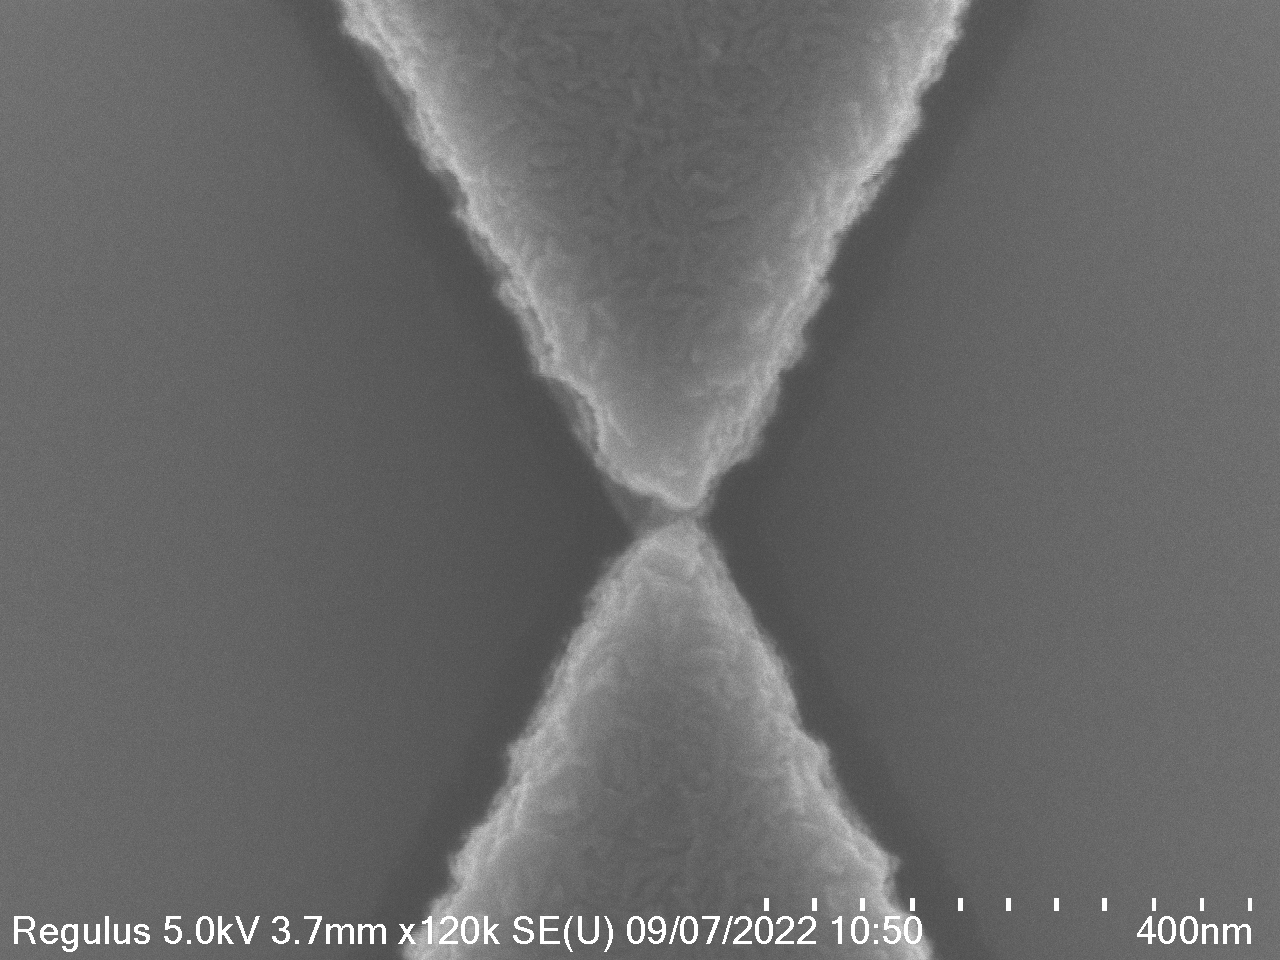
\includegraphics[width=\textwidth]{TiPdPdNbSEMBJ1_31_1300uCcm2_0003_1.png}
         %\caption{A cleaned substrate.\newline}
         %\label{a}
     \end{subfigure}
     \hfill
     \begin{subfigure}[b]{0.49\textwidth}
         \centering
         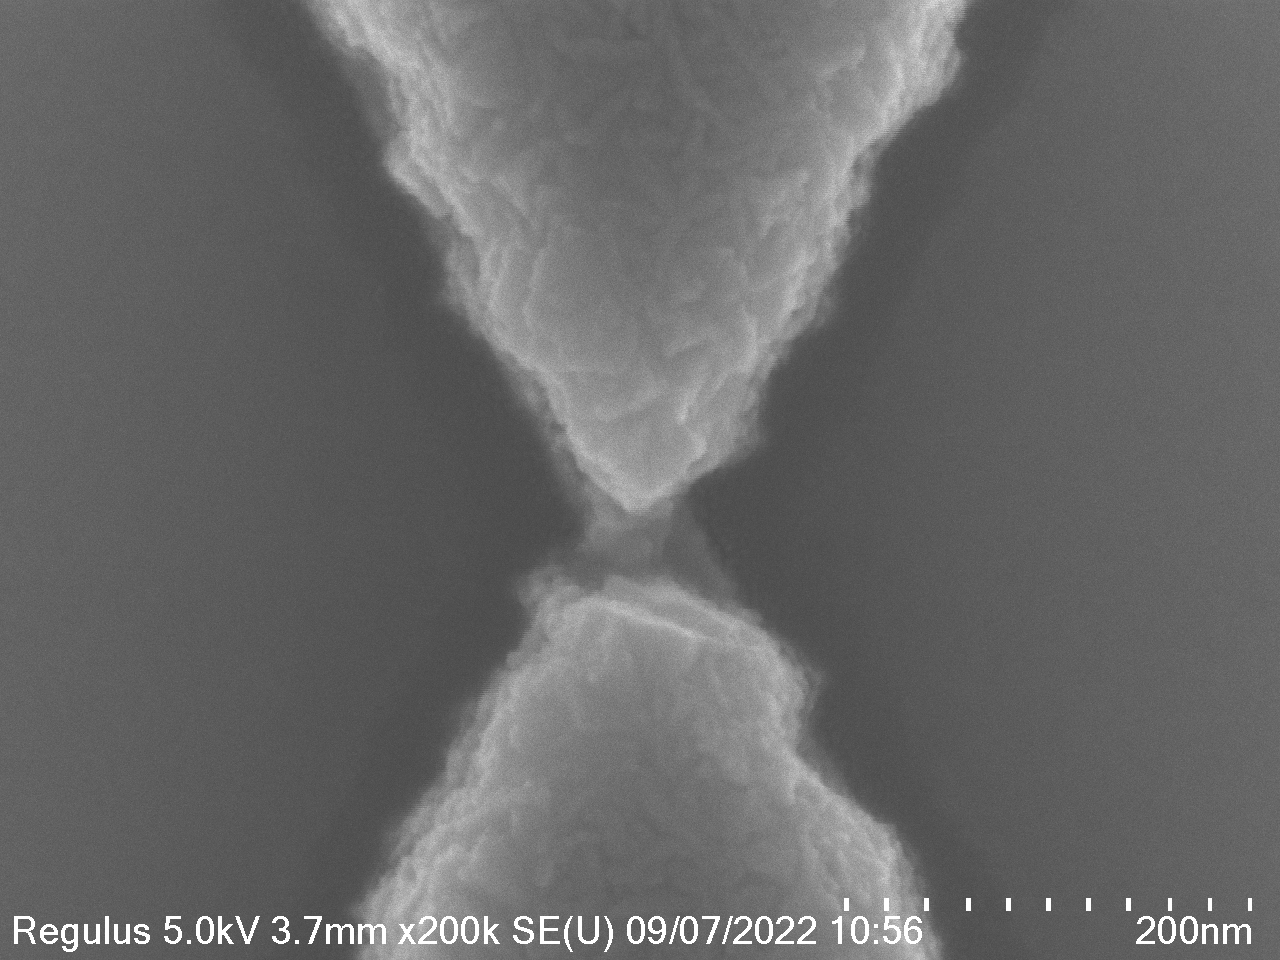
\includegraphics[width=\textwidth]{TiPdPdNbSEMBJ1_31_1320uCcm2_0001_1.png}
         %\caption{Layers of PMMA and MMA are added onto the resist by spin-coating.}
         %\label{b}
     \end{subfigure}
     \hfill
     \begin{subfigure}[b]{0.49\textwidth}
         \centering
         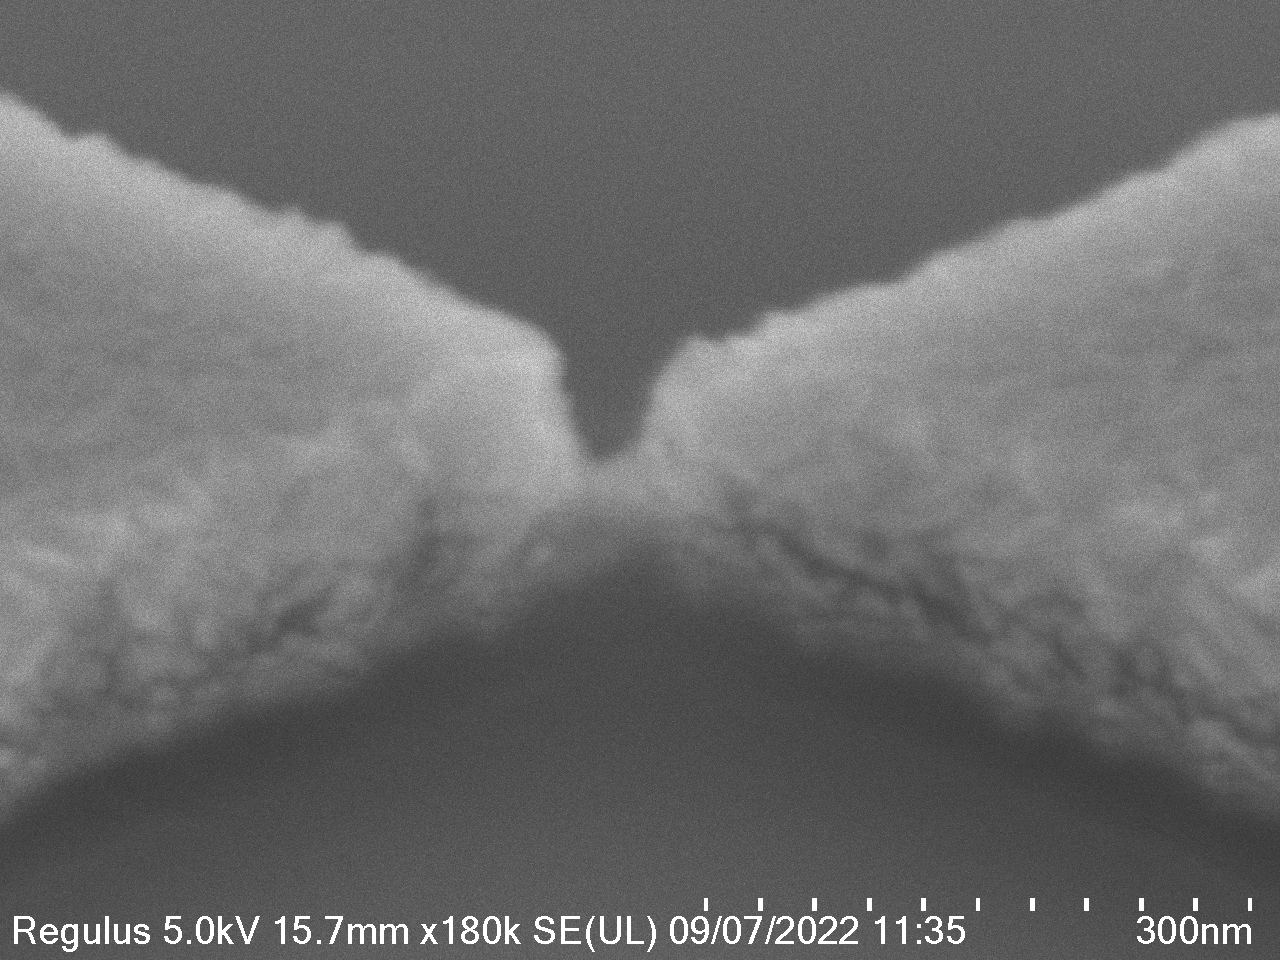
\includegraphics[width=\textwidth]{TiPdPdNbSEMBJ1_31_1320uCcm2_0013_1.png}
         %\caption{A portion of the resist is irradiated with an electron beam in as specified pattern.}
         %\label{c}
     \end{subfigure}
     \hfill
     \begin{subfigure}[b]{0.49\textwidth}
         \centering
         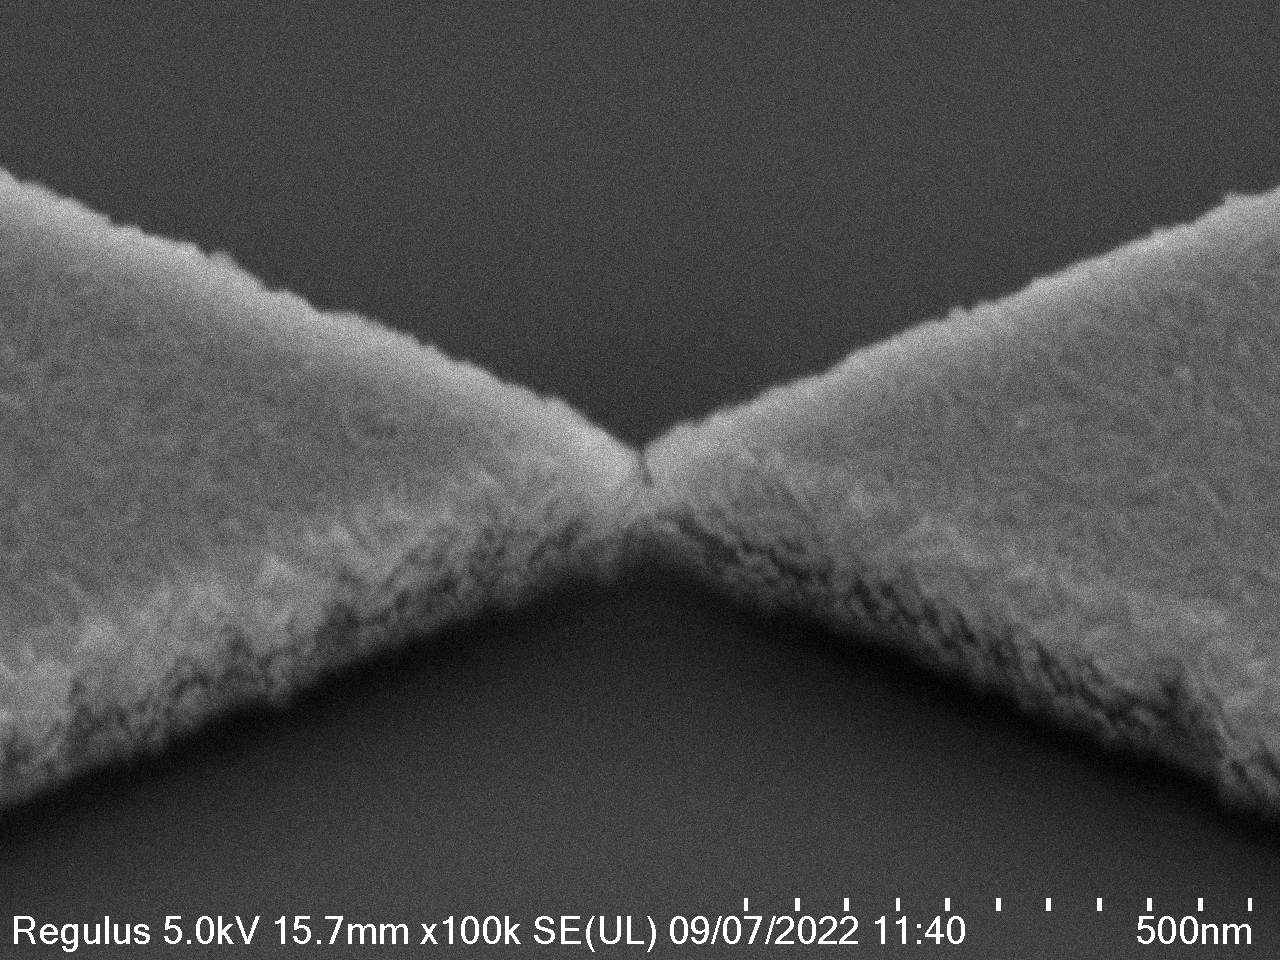
\includegraphics[width=\textwidth]{TiPdPdNbSEMBJ1_31_1340uCcm2_0002_1.png}
         %\caption{The irradiated region is dissolved away. \newline}
         %\label{d}
     \end{subfigure}
     \hfill
     \begin{subfigure}[b]{0.49\textwidth}
         \centering
         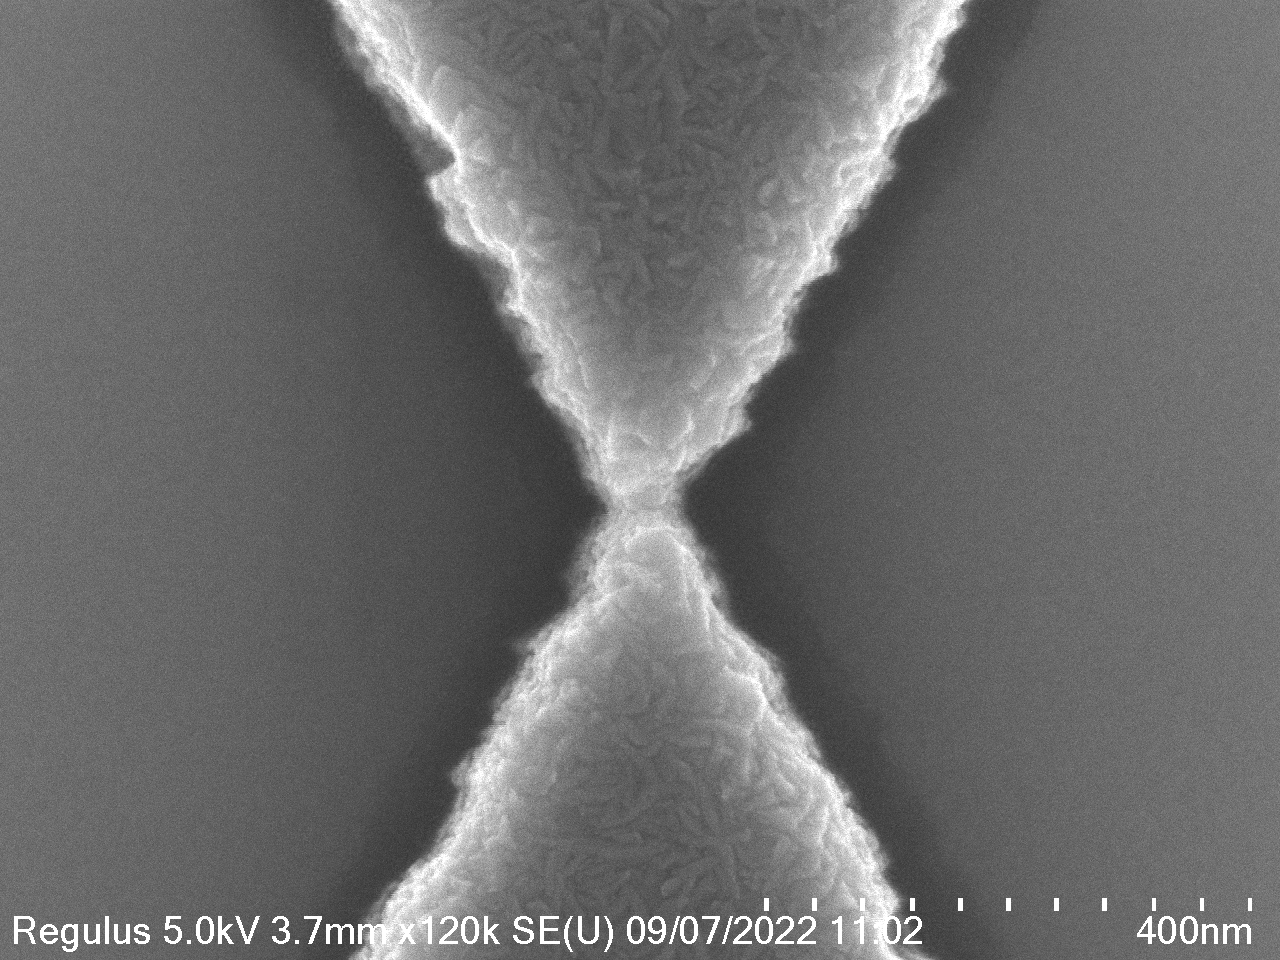
\includegraphics[width=\textwidth]{TiPdPdNbSEMBJ1_31_1660uCcm2_0002_1.png}
         %\caption{Material is evaporated onto the mask and substrate.}
         %\label{e}
     \end{subfigure}
     \hfill
     \begin{subfigure}[b]{0.49\textwidth}
         \centering
         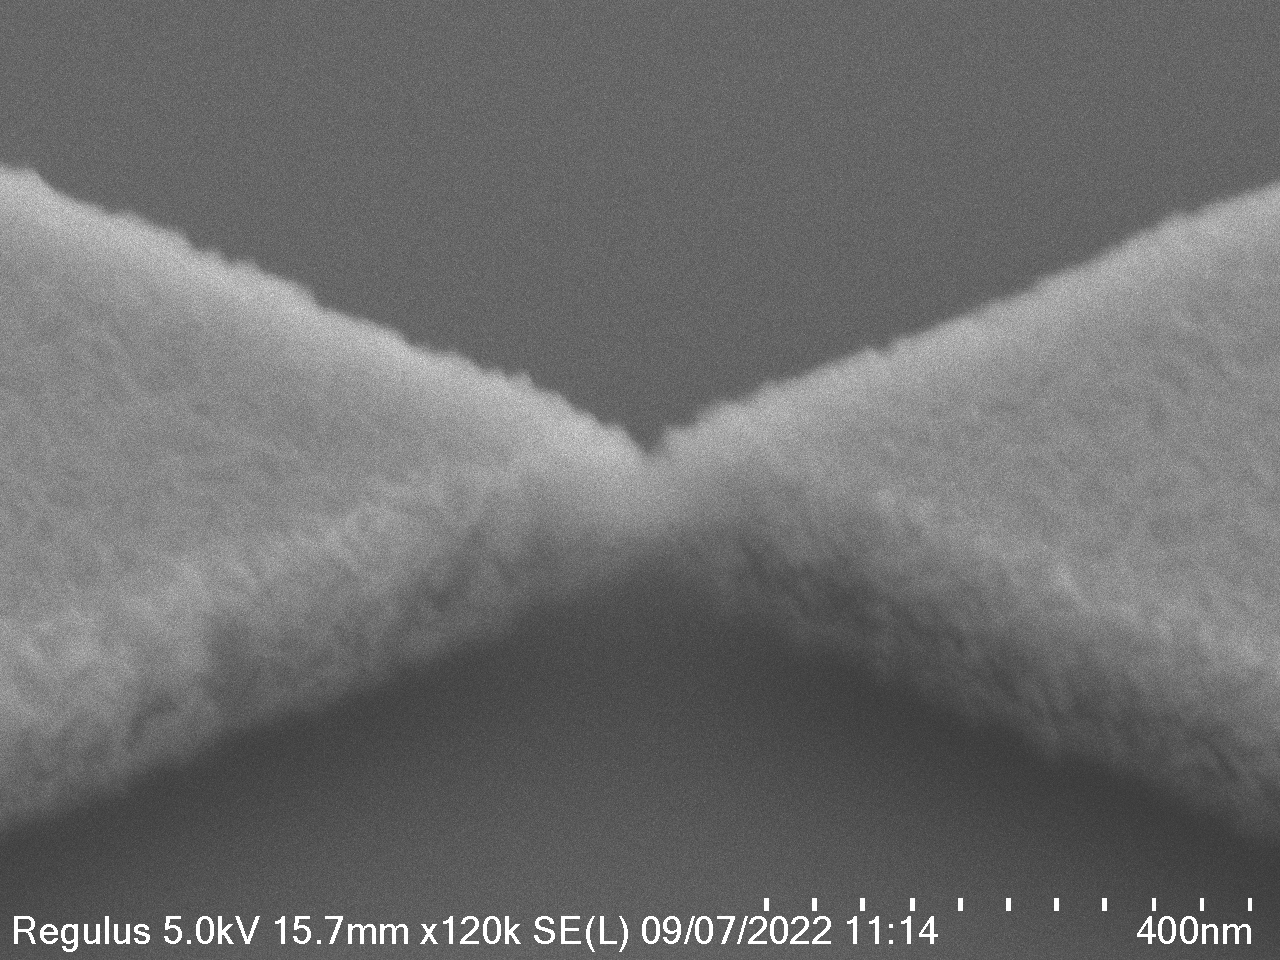
\includegraphics[width=\textwidth]{TiPdPdNbSEMBJ1_31_1660uCcm2_0006_1.png}
         %\caption{The mask is removed, leaving the patterned material on the substrate.}
         %\label{f}
     \end{subfigure}
        \caption{SEM images of 6 different palladium niobium based devices after fabrication. Some devices were imaged from the top, and others at an angle. Images taken by Damian Bouwmeester.}
        \label{fig:PdNb_fabrication_SEM}
        
\end{figure}

\subsubsection{AuNb}
In the next set of devices, all design parameters were kept the same with except for the bridge material, which was changed from palladium to gold. Figure \ref{fig:AuNb_SEM} shows two representative SEM images of these devices. For more examples, please refer to appendix A2. 

\begin{figure}[H]
     \centering
     \begin{subfigure}[t]{0.49\textwidth}
         \centering
         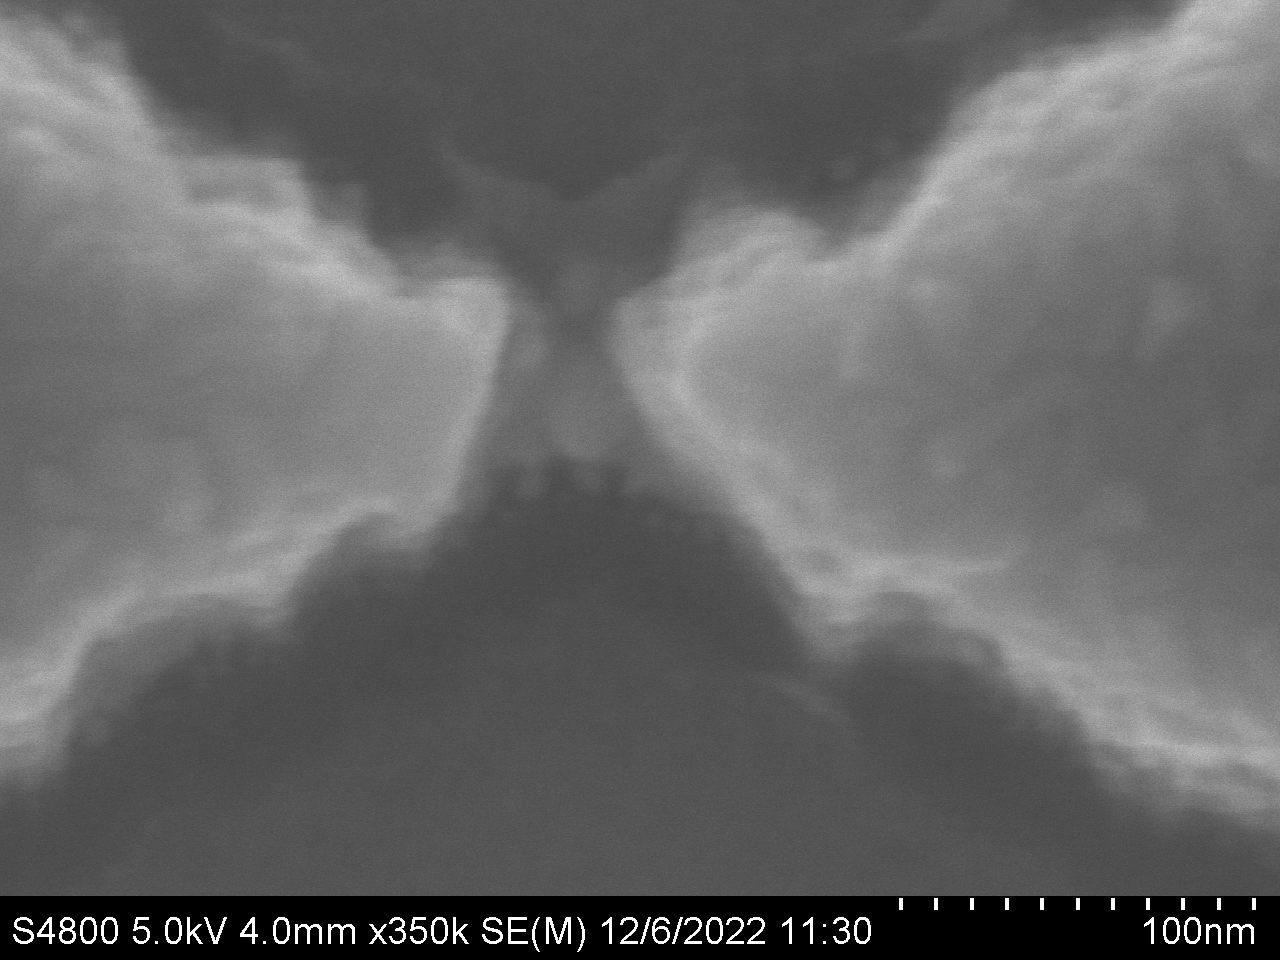
\includegraphics[width=\textwidth]{Appendix_A/A8.png}
         %\label{c}
     \end{subfigure}
     \hfill
     \begin{subfigure}[t]{0.49\textwidth}
         \centering
         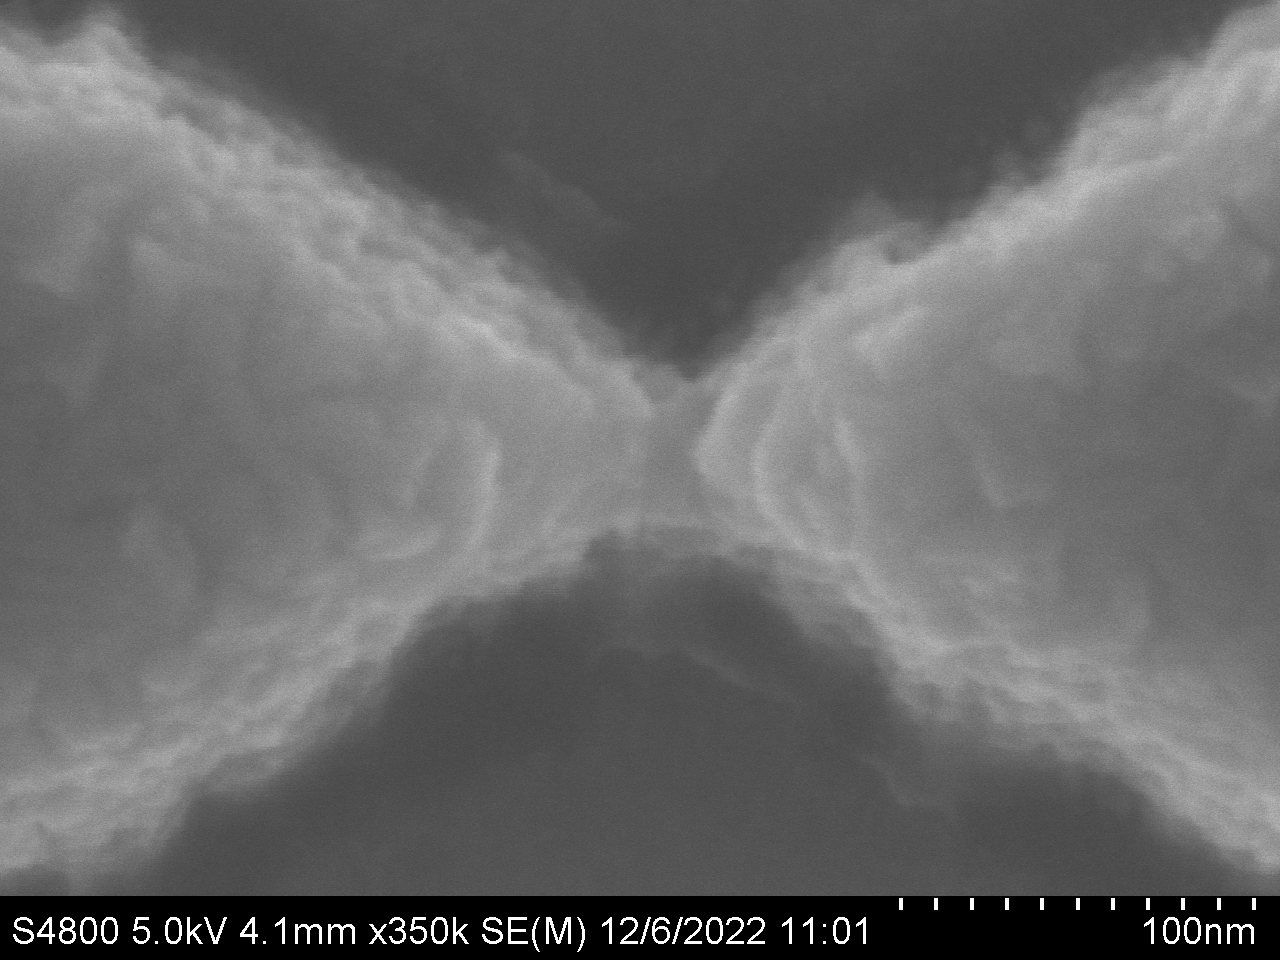
\includegraphics[width=\textwidth]{Appendix_A/E6.png}
         \label{subfig:Niobium_rates_comparison_50nm}
     \end{subfigure}
     
     \caption{SEM images of two AuNb devices. }
     \label{fig:AuNb_SEM}
        
\end{figure}

The SEM images of the AuNb devices show the same fabrication error as the PdNb device. In these devices the niobium layer is also not shaped as intended, with niobium overlapping the entire bridge in many devices.

\subsubsection{AuNb, 50 nm Nb}

The evaporation of 100 nm of niobium at a deposition rate of 0.2 nm/s led to a niobium layer that was inconsistent between devices, and even led to niobium bridging the entire junction in certain cases. It was hypothesized that by reducing the evaporation time, heating would be reduced and less film stress created, which would lead to a more consistent niobium layer with a shape that more closely matched that of the patterned mask. To test this hypothesis, new devices were fabricated whereby the thickness of the niobium layer was reduced to 50 nm and the evaporation rate increased to 0.5 nm/s. Figure \ref{fig:AuNbV3_SEM} depicts SEM images of devices made with 50 nm of niobium evaporated at 0.5 nm/s. For more such images, please refer to appendix A3.


\begin{figure}[H]
     \centering
     \begin{subfigure}[t]{0.49\textwidth}
         \centering
         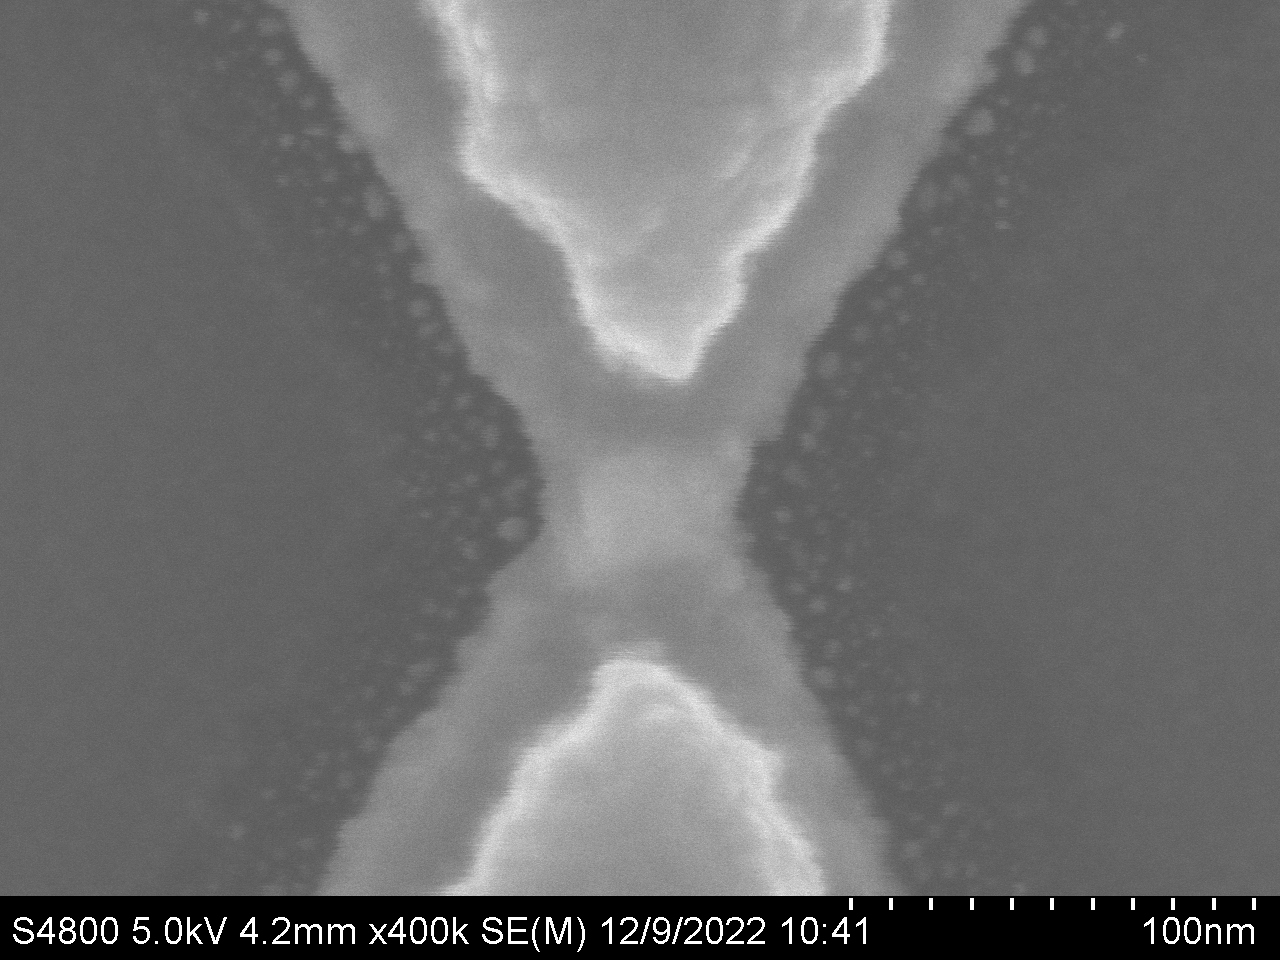
\includegraphics[width=\textwidth]{Appendix_A/A3/A2.png}
         %\label{c}
     \end{subfigure}
     \hfill
     \begin{subfigure}[t]{0.49\textwidth}
         \centering
         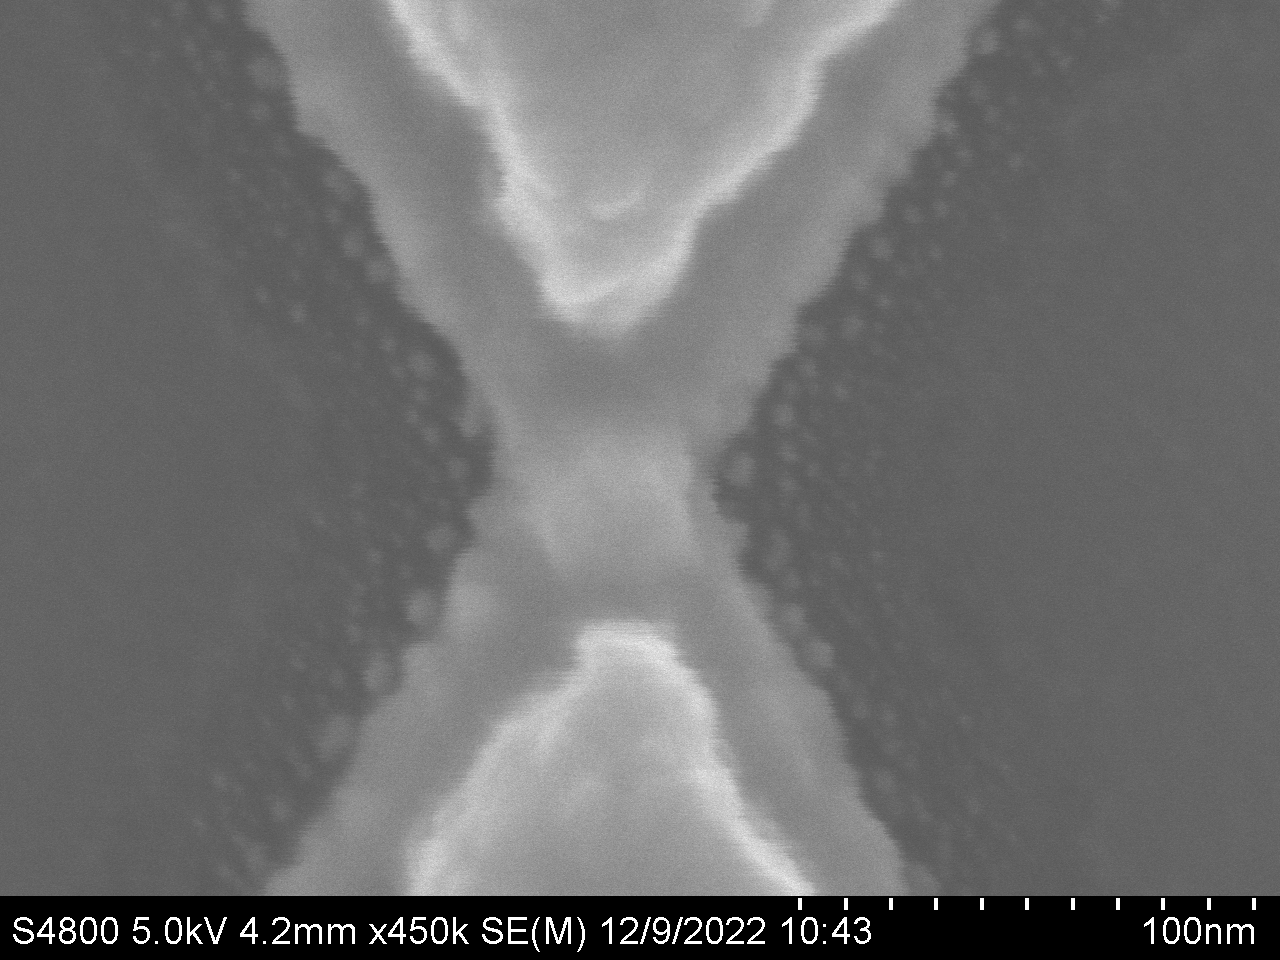
\includegraphics[width=\textwidth]{Appendix_A/A3/A3.png}
         \label{subfig:Niobium_rates_comparison_50nm}
     \end{subfigure}
     
     \caption{SEM images of AuNb devices with a niobium thickness of 50 nm and an evaporation rate of 0.5 nm/s.}
     \label{fig:AuNbV3_SEM}
        
\end{figure}

These SEM images show that with the new niobium evaporation parameters, the fabrication of the niobium layer is as intended.

\subsubsection{AuNb, 60 nm Bridge Spacing}

As can be seen in figure \ref{fig:AuNbV3_SEM} of the previous section, there is a region at the center of the junction where the two gold layers that were evaporated at different angles overlap. This overlap causes a region of lower current density and resistance, which makes electromigration less likely to happen in the center of the junction. A set of devices patterned with various junction spacings between 50 nm and 90 nm and exposed with the same dose as the previous device was fabricated in order to determine the spacing at which this overlap no longer occurs. The smallest spacing for which no overlap was seen on the SEM images was in those devices in which the patterned spacing was 60 nm. Based on this spacing test, a new set of devices was fabricated with a 60 nm bridge spacing pattern. Two of the SEM images taken for this set are shown in figure \ref{fig:AuNb60nm_SEM}. For more such images, please see appendix A4.


\begin{figure}[H]
     \centering
     \begin{subfigure}[t]{0.49\textwidth}
         \centering
         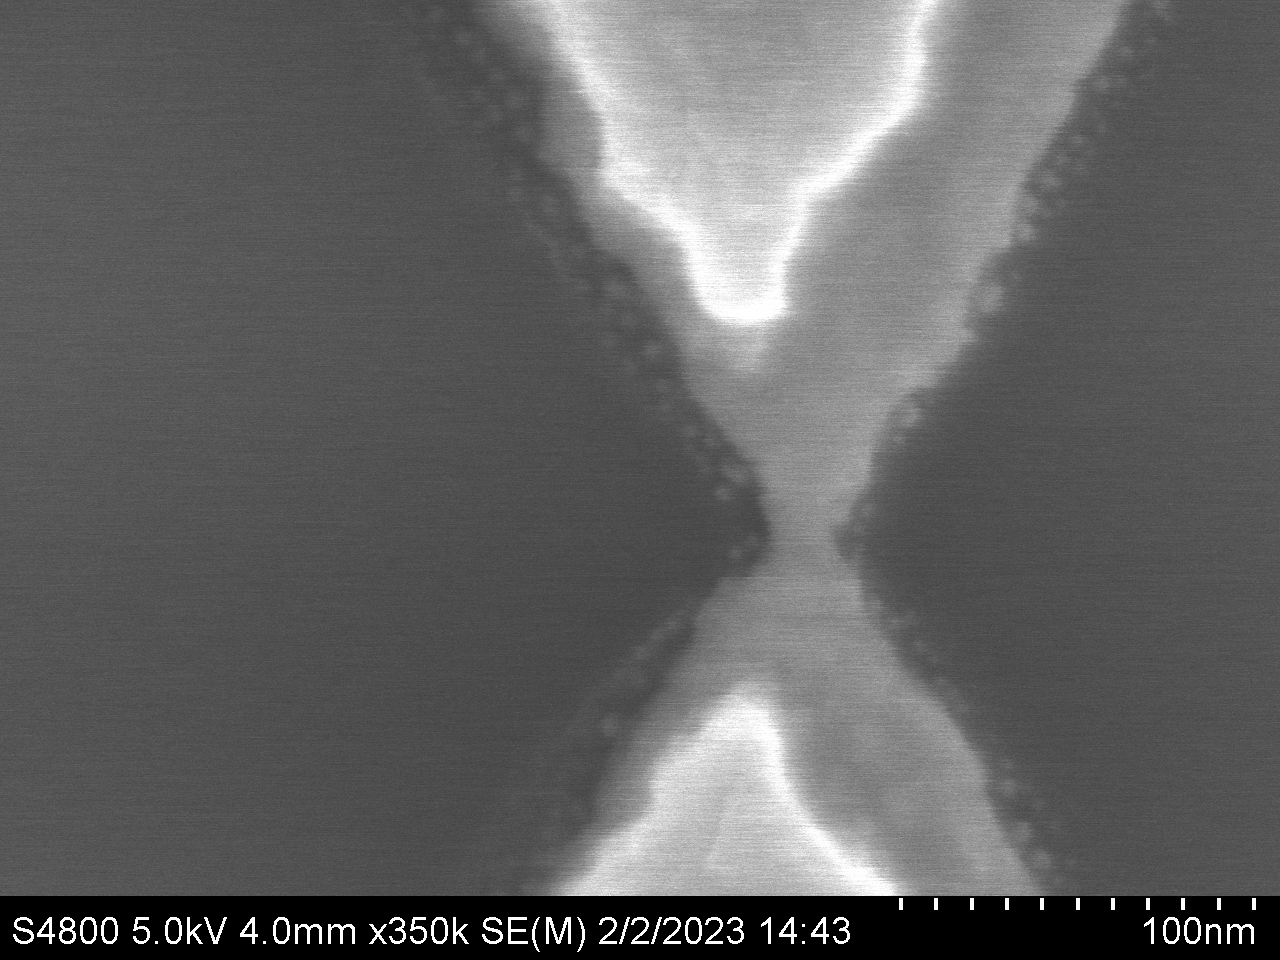
\includegraphics[width=\textwidth]{Appendix_A/A4/variousb360nm.png}
         %\label{c}
     \end{subfigure}
     \hfill
     \begin{subfigure}[t]{0.49\textwidth}
         \centering
         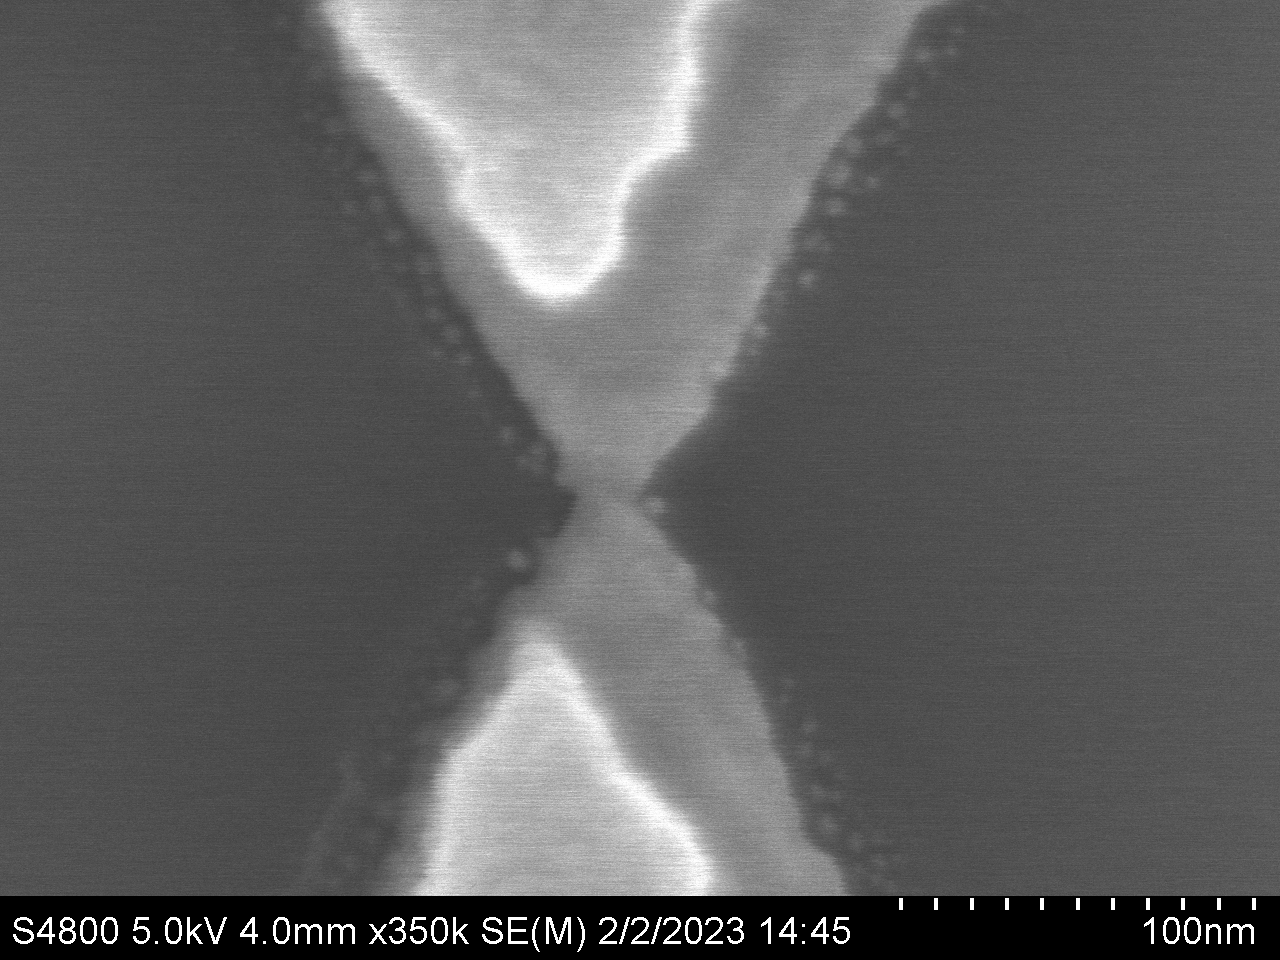
\includegraphics[width=\textwidth]{Appendix_A/A4/variousb460nm.png}
         \label{subfig:Niobium_rates_comparison_50nm}
     \end{subfigure}
     
     \caption{SEM images of AuNb devices with a bridge spacing of 60 nm.}
     \label{fig:AuNb60nm_SEM}
        
\end{figure}

There are important differences between the devices shown in these images and those shown in the previous section. The first of these is that the region of gold overlap in the center of the junction is no longer visible. The constriction has also become narrower in the center. Another difference that can be seen is the placement of the niobium layer. During the niobium evaporation, the samples were not placed in the center of the target. As a result, there is a slight translation of the niobium layer in the direction perpendicular to the wire. This is an unintended error in fabrication.

\subsection{Transport Before Electromigration}

The goal of this thesis is to optimize and characterize the devices after electromigration. By also performing transport measurements on the devices before electromigration we can extract information that helps us characterize the migration process and the devices after migration. Measurements on the devices before migration let us determine the $T_C$ of the bulk film and of the bridge, the normal state resistance of the bridge and the series resistance of the device, the critical current and an estimate of the Thouless energy before migration. The $T_C$ value of the bulk film is an important quantity that gives us information about the quality of the film, the strength of the (inverse) proximity effect in the bulk bilayer, and which is not expected to be altered by the migration process. The bridge and series resistance are important quantities for the migration process. By comparing the Thouless energy before and after migration, we can gain insight in the way the device properties are altered by migration. Therefore, measurements were also done on the devices before they were electromigrated.

\subsubsection{VI Measurements}

After fabrication, the devices of each design were loaded into either the dilution fridge or the dip-stick measurement set-up, and cooled down to a temperature between 25 mK and 1.6 K. Using a BEEP-R box resistance measurement device, the resistances of all devices were found to be of the order of 50 $\Omega$. In this resistance regime, we choose to do the transport measurements using the VI set-up, as discussed in the chapter on Methods. The measurements are done using a two probe configuration.

\subsubsection{PdNb}

In total, 16 devices with the PdNb design were loaded into the dilution fridge and cooled down to 1.2 K. 

For each of the 16 devices, a VI measurement was performed whereby the current was swept from -10 $\mu$A to 10 $\mu$A. A representative result of such a measurement, as well as a plot containing its numerical derivative, are shown in figure \ref{fig:VI_PdNb}. A single device had a critical current of more than 10 $\mu$A, which was therefore measured in the range between $\pm$20 $\mu$A. For a larger selection of measurement results, please consult appendix B1.


\begin{figure}[H]
     %These plots come from numid 2 from PdNb chip 6
     \begin{subfigure}[b]{0.49\textwidth}
         \centering
         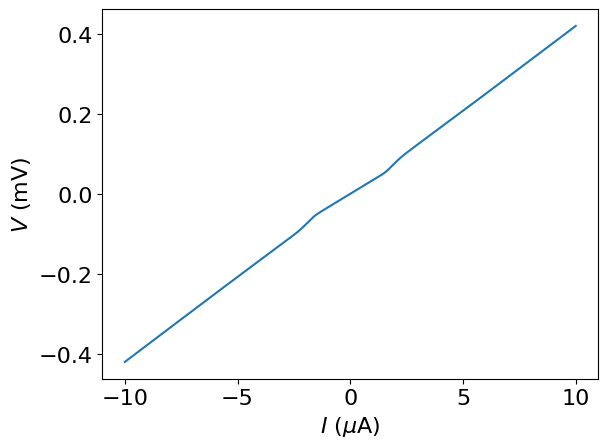
\includegraphics[width=\textwidth]{VI_PdNb_numid2.png}
         \caption{Representative current bias relationship at 1.2 K}
         \label{subfig:VI_PdNb}
     \end{subfigure}
     \hfill
     \begin{subfigure}[b]{0.47\textwidth}
         \centering
         \includegraphics[width=\textwidth]{dVdI_PdNb_numid2.png}
         \caption{Numerical derivative of the current bias relationship shown in figure (a).}
         \label{subfig:dVdI_PdNb}
     \end{subfigure}
        \caption{VI measurement and its derivative for a single device at 1.2 K.}
        \label{fig:VI_PdNb}
        
\end{figure}

We can extract the critical current from the differential resistance plot (figure \ref{subfig:dVdI_PdNb}), by extracting the argmax for both positive and negative currents, which we denote $I_c^+$ and $I_c^-$. By taking the average of the absolute values of $I_c^+$ and $I_c^-$, we get the critical current $I_c$. The extraction of $I_c^+$ and $I_c^-$ from the plot in figure \ref{subfig:dVdI_PdNb} is shown in figure \ref{fig:dVdI_PdNb_extractions}. In between $I_c^+$ and $I_c^-$ the bridge is superconducting, while outside this region it is not. By averaging the differential resistances in these regions, we can extract the device resistance while the bridge is in the normal state, which we denote $R_{n,d}$, and the device resistance while the bridge is in the superconducting state, denoted $R_s$. When performing these averages, the regions where the current is very close to either $I_c^+$ or $I_c^-$ are excluded, to account for the non-zero width of the differential resistance peaks. Since the bridge resistance is zero when the bridge is in the superconducting state, the normal state resistance of the bridge is given by $R_{n,d} - R_s$, and we symbolize it as $R_n$.

\begin{figure}[H]
     \centering
     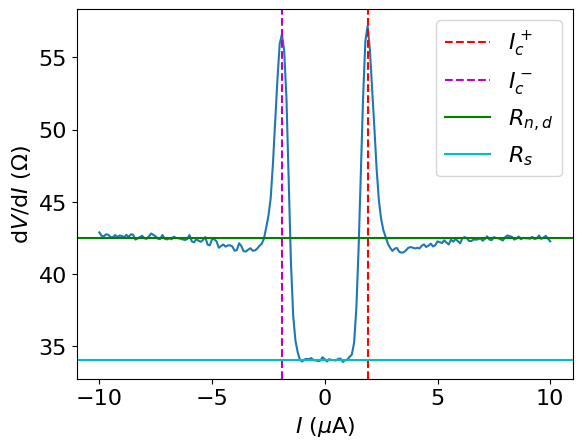
\includegraphics[width=0.8\textwidth]{dVdI_PdNb_numid2_extractions.png}
     \caption{A plot illustrating the extraction of $I_c^+$, $I_c^-$, $R_{n,d}$ and $R_s$ from the differential resistance. From these quantities we can calculate the critical current of the bridge, $I_c$ and the normal state resistance of the bridge $R_n$.}
     \label{fig:dVdI_PdNb_extractions}   
\end{figure}

Repeating this analysis for each of the 16 IV measurements, we can extract the $I_c$ and $R_n$ values for each device. These values have been plotted in figure \ref{fig:PdNb_IcRn_scatterplot}.

\begin{figure}[H]
     \centering  
     \begin{subfigure}[b]{0.8\textwidth}
         \centering
     	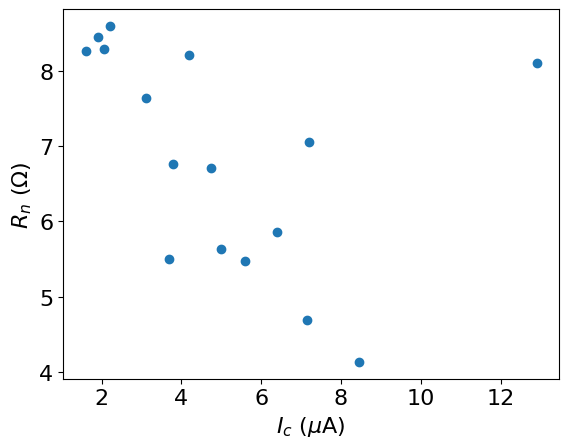
\includegraphics[width=\textwidth]{PdNb_IcRn_scatterplot.png}     	
     \end{subfigure}
     \caption{A scatterplot showing the value of the critical current, $I_c$, and the normal state bridge resistance, $R_n$, for each device.}
     \label{fig:PdNb_IcRn_scatterplot}
\end{figure}


\subsubsection{AuNb}

The AuNb devices were loaded into the dip-stick setup and cooled down to 2.1 K. 

VI measurements were performed on 4 devices. An exemplary result is shown in figure \ref{fig:AuNbV2_VI}, as well as a scatter plot showing the critical currents and normal state bridge resistances of the devices, which were extracted using the same method as before. For more measurement results, please see appendix B2.

\begin{figure}[H]
     %These plots come from numid 2 from PdNb chip 6
     \begin{subfigure}[t]{0.49\textwidth}
         \centering
         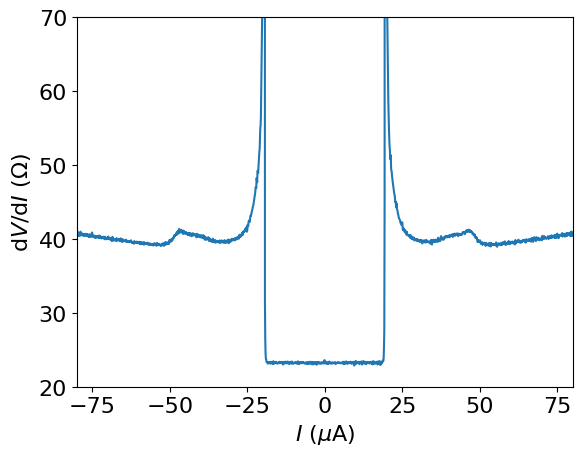
\includegraphics[width=\textwidth]{dVdI_AuNb_numid26.png}
         \caption{Numerical derivative of a representative VI measurement in an AuNb device. }
         \label{subfig:}
     \end{subfigure}
     \hfill
     \begin{subfigure}[t]{0.49\textwidth}
         \centering
         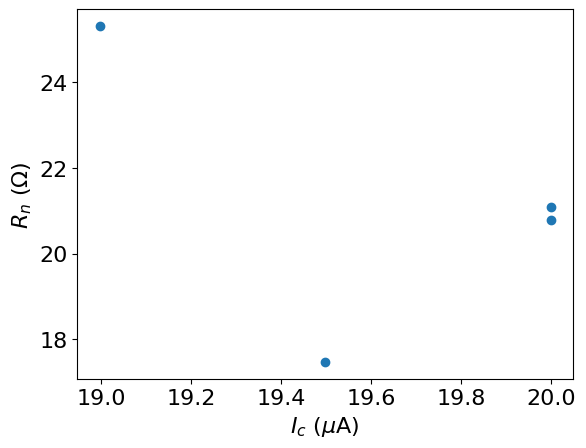
\includegraphics[width=\textwidth]{AuNb_IcRn_scatterplot.png}
         \caption{Extracted $I_C$ and $R_n$ values for AuNb devices.}
         \label{subfig:}
     \end{subfigure}
        \caption{Results from VI characterization of AuNb devices. Measurements performed at 2.1 K.}
        \label{fig:AuNbV2_VI}
        
\end{figure}

\subsubsection{AuNb, 50 nm Nb}
Of the AuNb devices with 50 nm of Nb, one set was loaded into the dip-stick setup and cooled to 1.9 K, while another set was loaded into the dilution fridge. In the dilution fridge, VI measurements were performed at approximately 5 K for 7 devices. A representative VI measurement, as well as a scatterplot showing the critical currents and normal state resistances, is shown in figure \ref{fig:AuNbV3_VI}. For more measurement results, refer to appendix B3.

\begin{figure}[H]
     %These plots come from numid 2 from PdNb chip 6
     \begin{subfigure}[t]{0.49\textwidth}
         \centering
         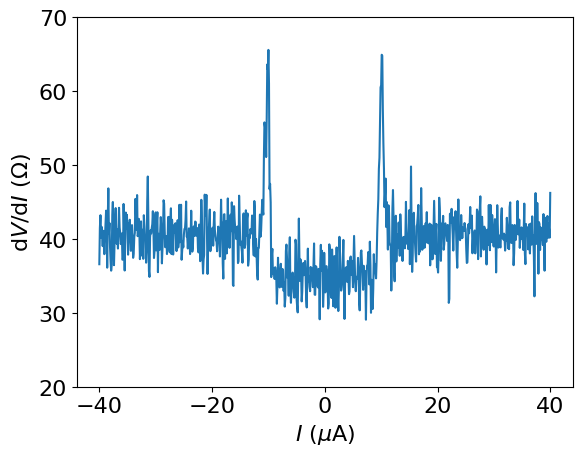
\includegraphics[width=\textwidth]{Appendix_B/B3/dVdI_AuNbV3DF_numid12.png}
         \caption{Numerical derivative of a representative VI measurement in an AuNb device with 50 nm thick niobium.}
         \label{subfig:}
     \end{subfigure}
     \hfill
     \begin{subfigure}[t]{0.49\textwidth}
         \centering
         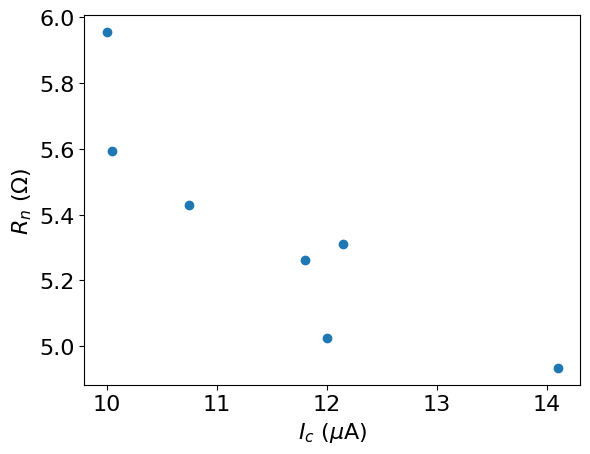
\includegraphics[width=\textwidth]{AuNbV3DF_IcRn_scatterplot.png}
         \caption{Extracted $I_C$ and $R_n$ values for AuNb devices with 50 nm thick niobium.}
         \label{subfig:}
     \end{subfigure}
        \caption{Results from VI characterization of AuNb devices with 50 nm thick niobium. Measurements performed at approximately 5 K.}
        \label{fig:AuNbV3_VI}
        
\end{figure}

\subsubsection{AuNb, 60 nm Spacing}

The AuNb devices with 60 nm bridge spacing were loaded into the dilution fridge, and cooled down to 25 mK. At this temperature, the retrapping current is different from the critical current. Therefore, the current was swept first from 0 in the positive direction, and then from 0 in the negative direction. When sweeping the current in this way, we obtain the critical currents and not the retrapping current. A representative VI measurement, as well as a scatterplot showing the critical currents and normal state resistances, is shown in figure \ref{fig:AuNb60nm_VI}. More results are shown in appendix B4.

\begin{figure}[H]
     %These plots come from numid 2 from PdNb chip 6
     \begin{subfigure}[t]{0.49\textwidth}
         \centering
         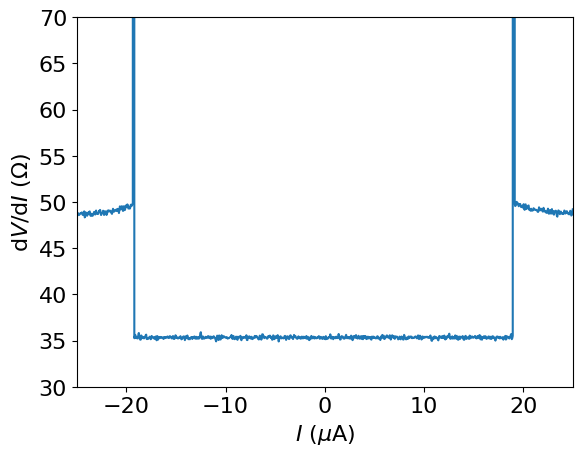
\includegraphics[width=\textwidth]{dVdI_AuNb60_numid57.png}
         \caption{Numerical derivative of a representative VI measurement in an AuNb device with 60 nm bridge spacing. }
         \label{subfig:}
     \end{subfigure}
     \hfill
     \begin{subfigure}[t]{0.49\textwidth}
         \centering
         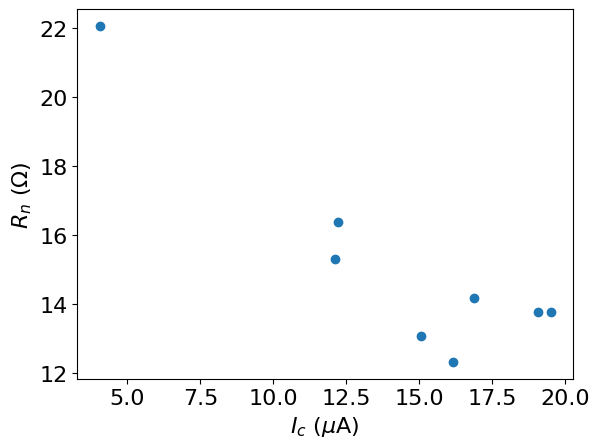
\includegraphics[width=\textwidth]{AuNb60_IcRn_scatterplot.png}
         \caption{Extracted $I_C$ and $R_n$ values for AuNb devices with 60 nm bridge spacing.}
         \label{subfig:}
     \end{subfigure}
        \caption{Results from VI characterization of AuNb devices with 60 nm bridge spacing. Measurements performed at approximately 25 mK.}
        \label{fig:AuNb60nm_VI}
        
\end{figure}



\subsection{Temperature Dependence Measurements}

The temperature dependence of the transport properties of the junctions gives us information that is used in the discussion chapter to analyze the quality of the devices. Since the devices all have resistances of the order of 50$\Omega$, VIT measurements were chosen as the method for investigating the temperature dependence of the unbroken junctions. The results of these VIT measurements are shown in this section.

\subsubsection{PdNb}

In order to measure the temperature dependence of the PdNb devices, a single VIT measurement was performed on a single device. The current was swept in the range of $\pm$5 $\mu$A, while the temperature of the device was raised from 1.6 K to 9 K. The measurement result is shown in figure \ref{fig:VIT_PdNb}. The size of the temperature increments between IV traces was not constant, and was largest between 2 K and 3 K. As a result, the temperature resolution of the measurement in this region is lower. By averaging the differential resistance over a small interval around 0 current, we get the zero current temperature dependence of the differential resistance. 

\begin{figure}[H]
     %These plots come from numid 2 from PdNb chip 6
     \begin{subfigure}[t]{0.49\textwidth}
         \centering
         \includegraphics[width=\textwidth]{PdNb_VIT.png}
         \caption{VIT measurement from 1.6 K to 9 K.}
         \label{subfig:VIT_PdNb}
     \end{subfigure}
     \hfill
     \begin{subfigure}[t]{0.47\textwidth}
         \centering
         \includegraphics[width=\textwidth]{PdNb_dVdIT.png}
         \caption{Numerical derivative of the voltage with respect to the bias current of the graph shown in figure (a).}
         \label{subfig:dVdIT_PdNb}
     \end{subfigure}
     \hfill
     \centering
     \begin{subfigure}[t]{0.47\textwidth}
         \centering
         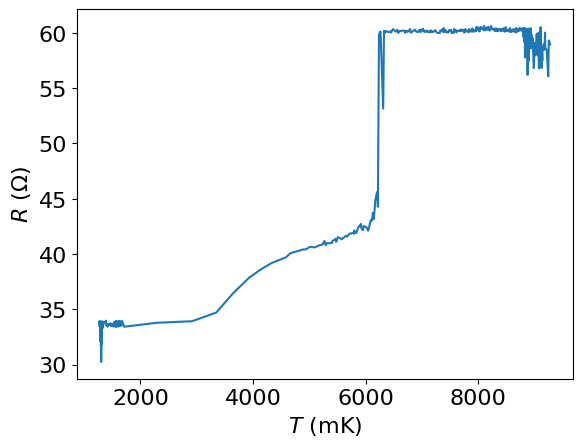
\includegraphics[width=\textwidth]{PdNb_RT.png}
         \caption{Differential resistance of the junction, averaged over a small current interval around zero as a function of temperature.}
         \label{subfig:dVdIT_PdNb}
     \end{subfigure}
        \caption{VIT measurement results for PdNb device.}
        \label{fig:VIT_PdNb}
        
\end{figure}


\subsubsection{AuNb, 100 nm Nb and 50 nm Nb}

A VIT measurement similar to the one done for the PdNb devices was done for the AuNb devices, both those with 100 nm Nb and those with 50 nm Nb. These measurements were done in the dip-stick setup. The results are shown in figures \ref{fig:AuNbV2_VIT} and \ref{fig:AuNbV3_VIT} respectively.

\begin{figure}[H]
     %These plots come from numid 2 from PdNb chip 6
     \begin{subfigure}[b]{0.55\textwidth}
         \centering
         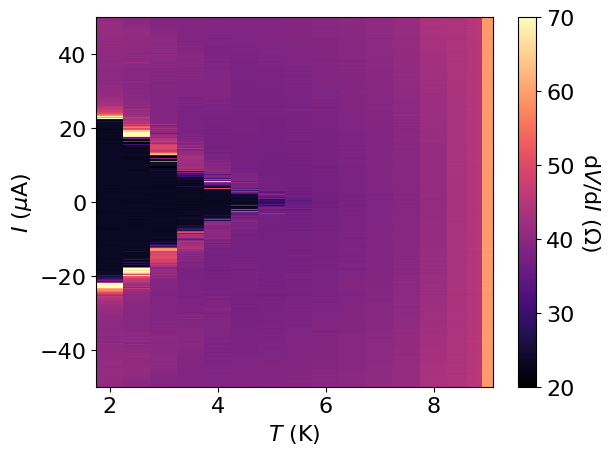
\includegraphics[width=\textwidth]{AuNbV2_VIT.png}
         \caption{Representative VIT }
         \label{subfig:}
     \end{subfigure}
     \hfill
     \begin{subfigure}[b]{0.45\textwidth}
         \centering
         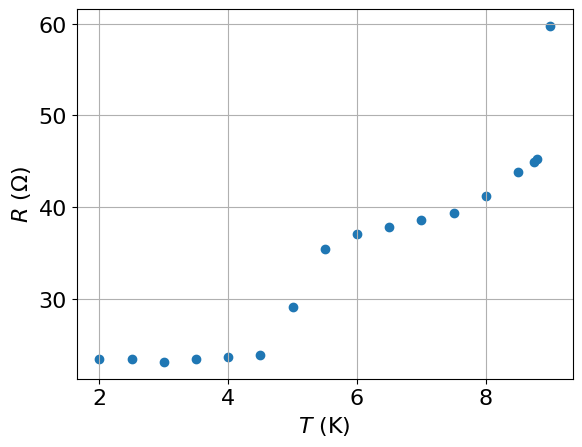
\includegraphics[width=\textwidth]{AuNbV2_RT.png}
         \caption{Zero bias current differential resistance as a function of temperature.}
         \label{subfig:}
     \end{subfigure}
        \caption{VIT measurement AuNb device.}
        \label{fig:AuNbV2_VIT}
        
\end{figure}

\begin{figure}[H]
     %These plots come from numid 2 from PdNb chip 6
     \begin{subfigure}[b]{0.55\textwidth}
         \centering
         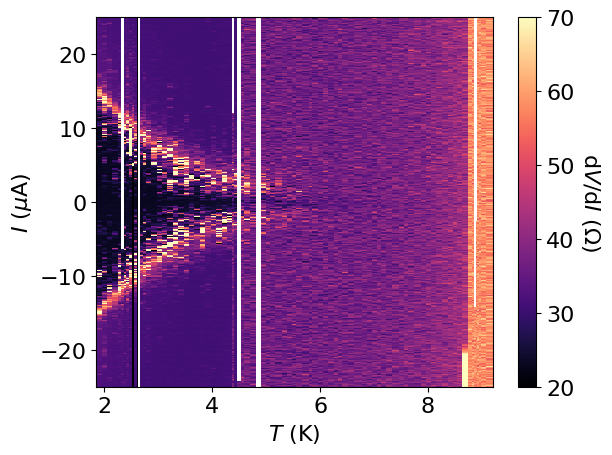
\includegraphics[width=\textwidth]{Appendix_C/C3/AuNbV3_dVdIT.png}
         \caption{Representative VIT }
         \label{subfig:}
     \end{subfigure}
     \hfill
     \begin{subfigure}[b]{0.45\textwidth}
         \centering
         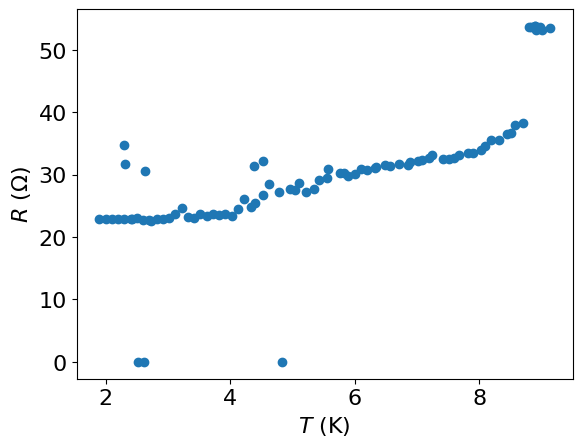
\includegraphics[width=\textwidth]{AuNbV3_RT.png}
         \caption{Zero bias current differential resistance as a function of temperature.}
         \label{subfig:}
     \end{subfigure}
        \caption{VIT measurement AuNb device with 50 nm thick niobium layer.}
        \label{fig:AuNbV3_VIT}
        
\end{figure}

Furthermore, another VIT measurement was performed on those AuNb devices with 50 nm Nb that were measured in the dilution fridge. This VIT has higher resolution and a lower temperature range, and is shown in figure \ref{fig:AuNbV3DF_VIT}.

\begin{figure}[H]
\centering
     %These plots come from numid 2 from PdNb chip 6
     \begin{subfigure}[b]{0.55\textwidth}
         \centering
         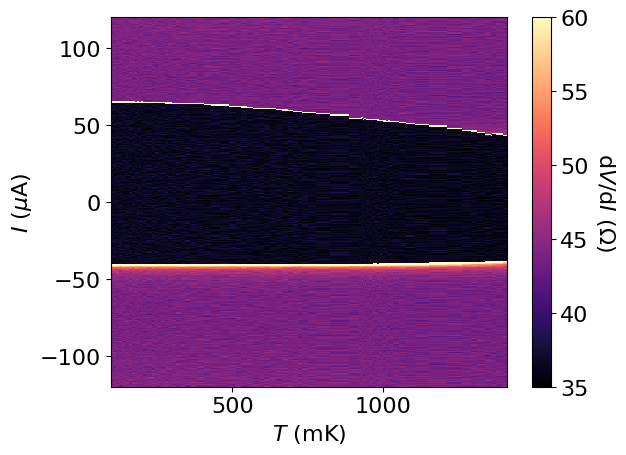
\includegraphics[width=\textwidth]{Appendix_C/C3/AuNbV3DF_dVdIT.png}
         \label{subfig:}
     \end{subfigure}
     
        \caption{VIT measurement AuNb device with 50 nm thick niobium layer.}
        \label{fig:AuNbV3DF_VIT}
        
\end{figure}


\subsubsection{AuNb, 60 nm Spacing}
For the devices with 60 nm spacing, no VIT measurement was performed. However, for some devices a VI measurement was performed at two or three different temperatures, which still allows us to extract some temperature dependence information. One such result is shown in figure \ref{fig:AuNb60nm_VIT}, and more are shown in appendix C4.


\begin{figure}[H]
     %These plots come from numid 2 from PdNb chip 6
     \begin{subfigure}[t]{0.49\textwidth}
         \centering
         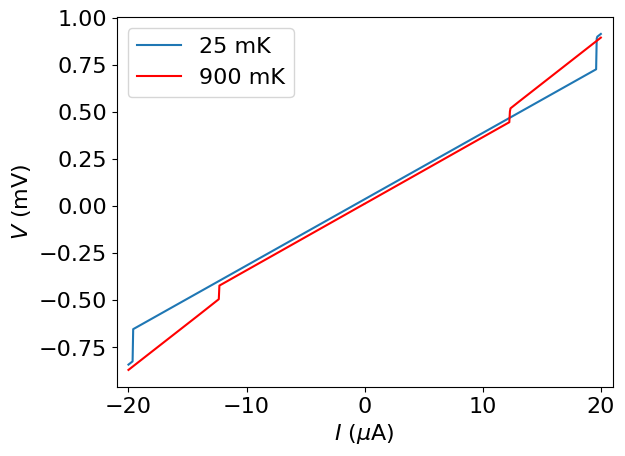
\includegraphics[width=\textwidth]{Appendix_C/C4/AuNb60nm_VIT_A6.png}
         \caption{Two VI measurements of the same AuNb device with 60 nm bridge spacing, taken at two different temperatures. }
         \label{subfig:}
     \end{subfigure}
     \hfill
     \begin{subfigure}[t]{0.49\textwidth}
         \centering
         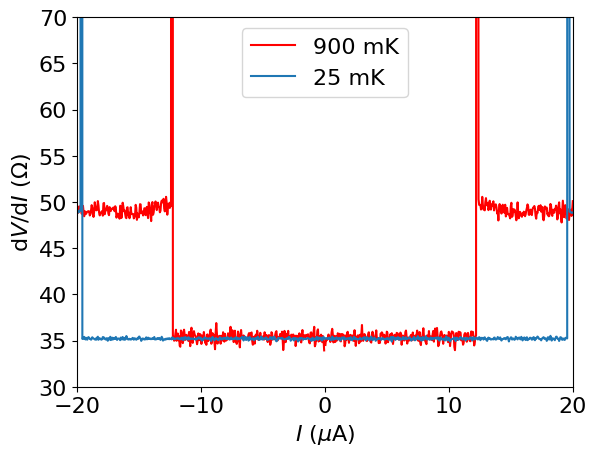
\includegraphics[width=\textwidth]{Appendix_C/C4/AuNb60nm_dVdIT_A6.png}
        \caption{Numerical derivative of the VI results in panel (a).}
         \label{subfig:}
     \end{subfigure}
        \caption{Temperature dependence of VI measurement of AuNb device with 60 nm bridge spacing.}
        \label{fig:AuNb60nm_VIT}
        
\end{figure}



\subsection{Electromigration}

All devices studied in this thesis were electromigrated using feedback controlled electromigration. A representative sample of the current bias relations and resistance curves obtained during electromigration are shown for devices of each type in appendix E.

The AuNb devices with 100 nm thick and 50 nm thick niobium were migrated at room temperature. The rest of the devices was migrated while the device was cooled. The target resistance was always set in the range between 1 $R_Q$ = 12.9 k$\Omega$, and 50k$\Omega$. Table \ref{fig:Migration_stats} shows the migration statistics, as measured by the BEEP-R box. The resistances were measured separately both while the devices were at room temperature and while they were cooled down, as indicated by the color of the data points.

Significantly, some of the devices showed an increase in resistance when they were cooled down which reversed once the devices were warmed back up to room temperature.

\begin{figure}[H]
\centering
     %These plots come from numid 2 from PdNb chip 6
     \begin{subfigure}[b]{0.8\textwidth}
         \centering
         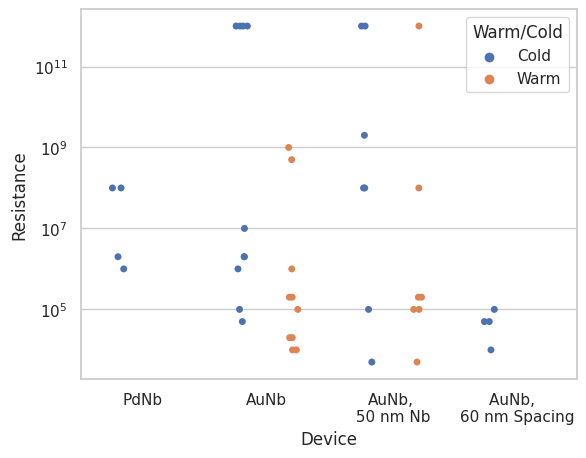
\includegraphics[width=\textwidth]{Migration_stats.png}
         \label{subfig:}
     \end{subfigure}
     
        \caption{BEEP-R box characterization of device resistances after migration. For some device types, the resistance was measured both at room temperature directly after warm electromigration and at low temperature.}
        \label{fig:Migration_stats}
        
\end{figure}

In figure \ref{fig:Migrated_SEMs} below, one representative electromigrated junction of each gold-bridged device type is shown.

\begin{figure}[H]
     %These plots come from numid 2 from PdNb chip 6
     \begin{subfigure}[t]{\textwidth}
         \centering
         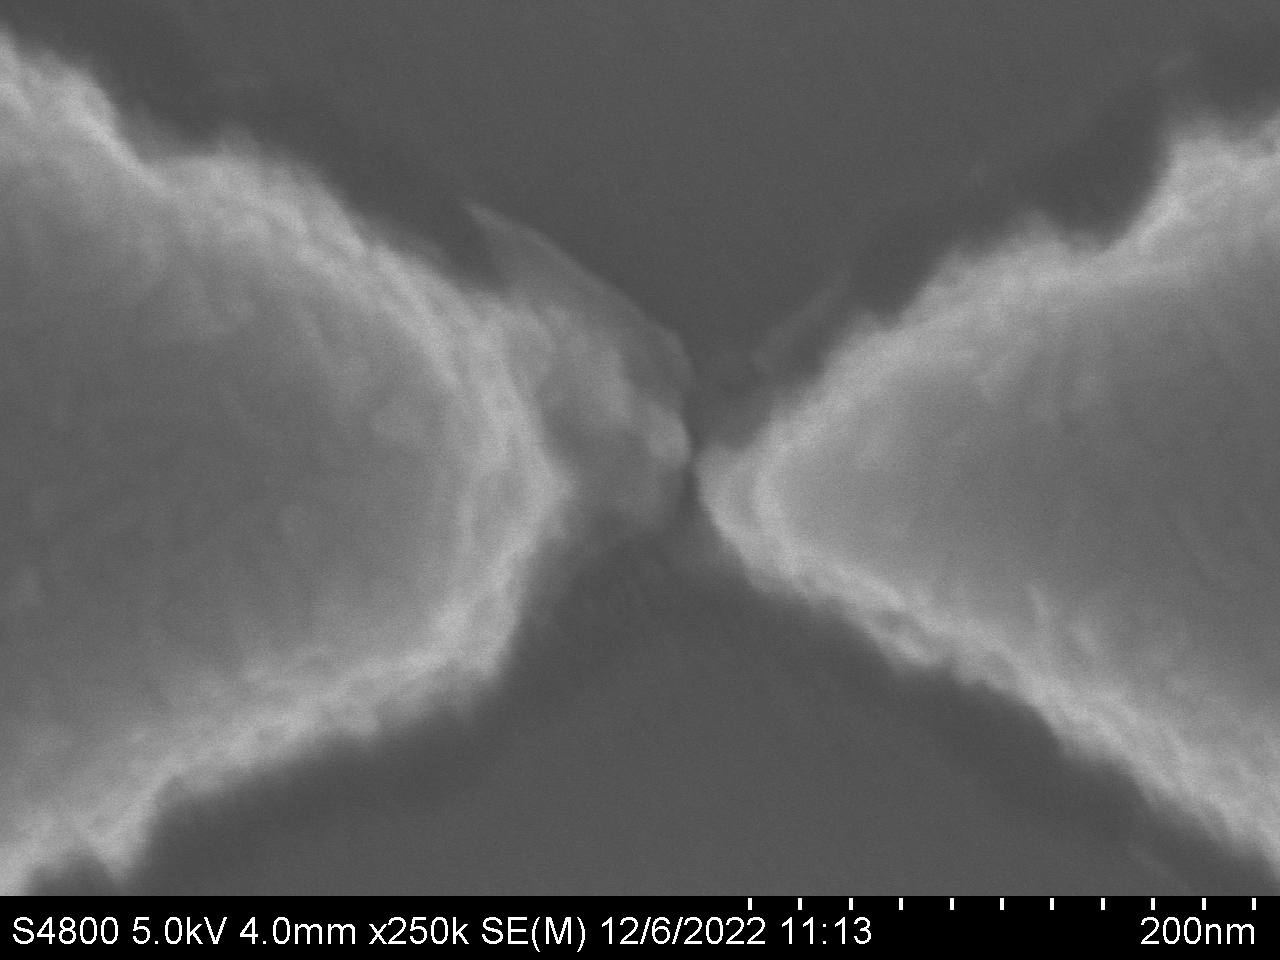
\includegraphics[width=0.49\textwidth]{AuNbV2_After_Migration.png}
         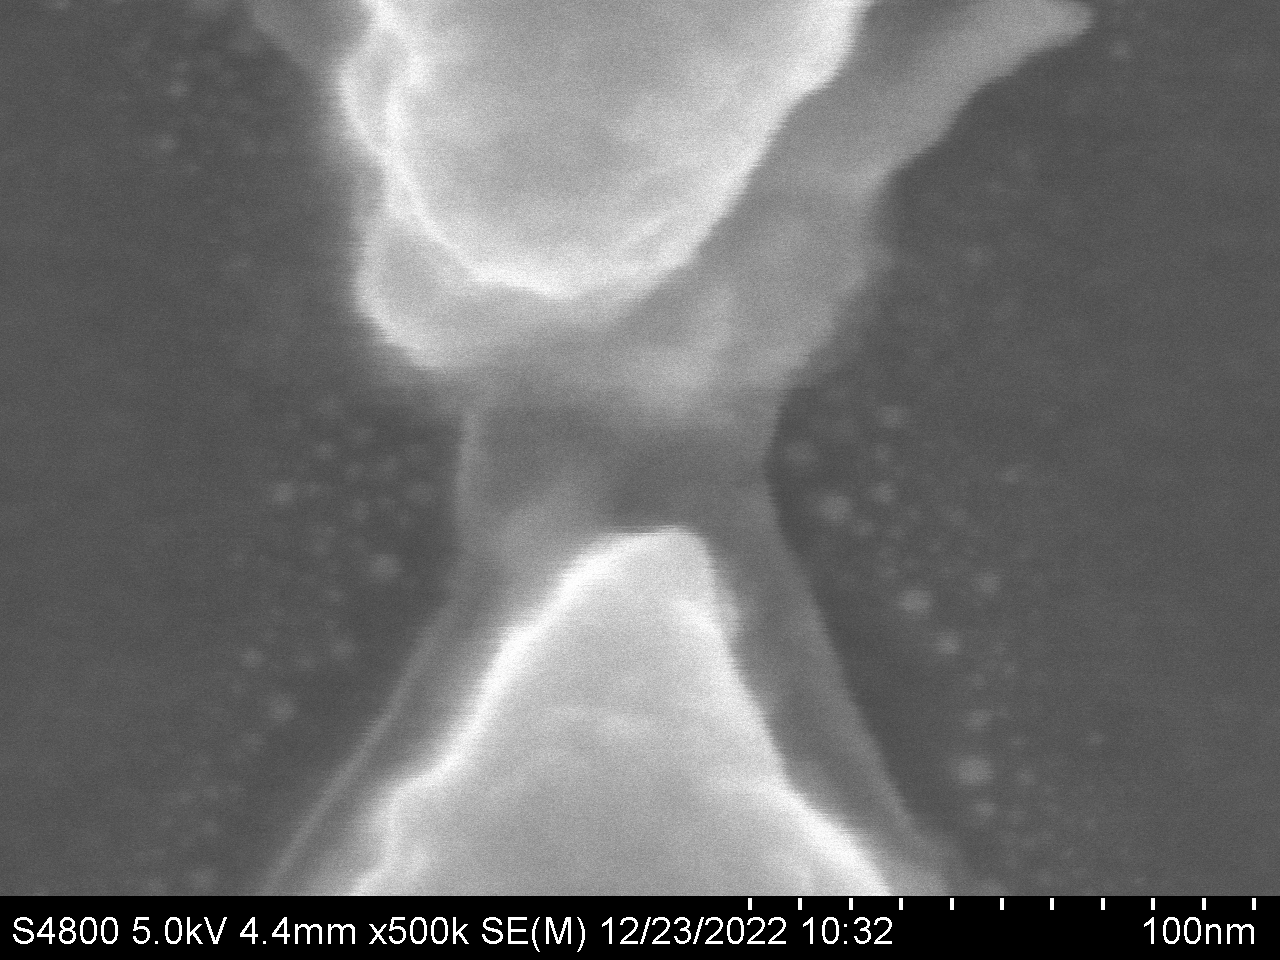
\includegraphics[width=0.49\textwidth]{AuNbV3_After_Migration.png}
         %\label{subfig:bistable_IV}
     \end{subfigure}
     \hfill
     \begin{subfigure}[t]{\textwidth}
         \centering
         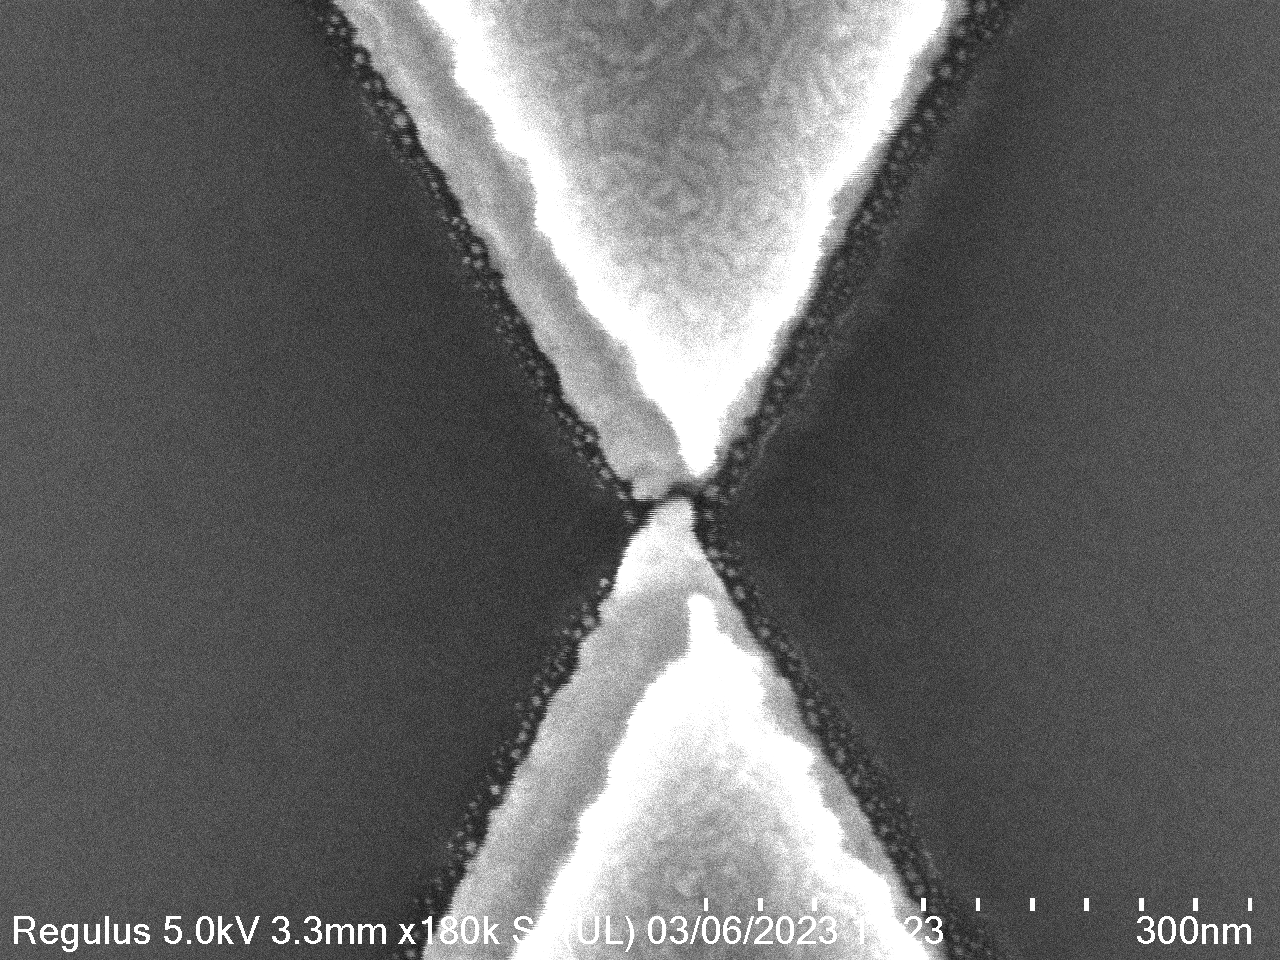
\includegraphics[width=0.49\textwidth]{AuNb60nmAfterMigration.png}
     \end{subfigure}
        \caption{SEM images of devices after electromigration. The device types are: AuNb (top left), AuNb with 50 nm Nb (top right), and AuNb with 60 nm bridge spacing (bottom).}
        \label{fig:Migrated_SEMs}
        
\end{figure}

All but one of the AuNb devices with 60 nm bridge spacing were destroyed during the measurements via gate leakage. The only device that wasn't destroyed completely was still altered by gate leakage, since the resistance changed from 50 k$\Omega$ before the gate leakage to a resistance reading of 'Open' after the gate leakage, as measured by a BEEP-R box. Therefore, the size of the gap in this image is likely larger than it was during the operational conditions of this device, and it is not certain that the SEM image above is representative of all the broken devices of this type in terms of the location of the gap or its shape.

\subsection{Transport After Electromigration}
For all of the broken junctions that were studied, an IV measurement was performed. If the measurement contained a suppression of the differential conductance around zero bias that might be due to superconductivity, the temperature or the magnetic field was raised past its critical value in order to validate that the suppression was the result of superconductivity. In the dip stick setup, no magnet is available, and the temperature can be controlled using a heater, so in that set up a temperature dependent measurement would be chosen for the validation. In the dilution fridge a magnet is available and magnetic field dependent measurements would be used for the validation.



\subsubsection{PdNb}
Four devices were migrated, and for each of these devices an IV measurement was performed. Two such measurements are shown in figure \ref{fig:PdNb_IV}, and others can be found in appendix F.

         
\begin{figure}[H]
     %These plots come from numid 2 from PdNb chip 6
     \begin{subfigure}[t]{\textwidth}
         \centering
         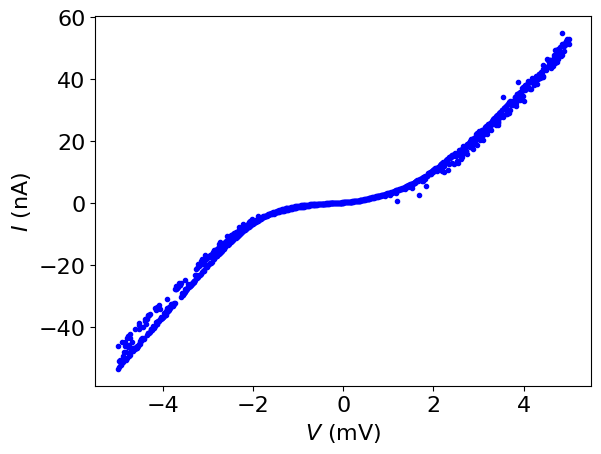
\includegraphics[width=0.49\textwidth]{IV_96.png}
         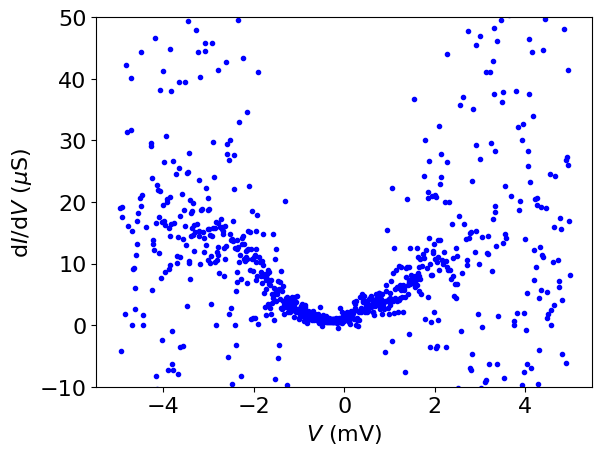
\includegraphics[width=0.49\textwidth]{dIdV_96.png}
         %\label{subfig:bistable_IV}
     \end{subfigure}
     \hfill
     \begin{subfigure}[t]{\textwidth}
         \centering
         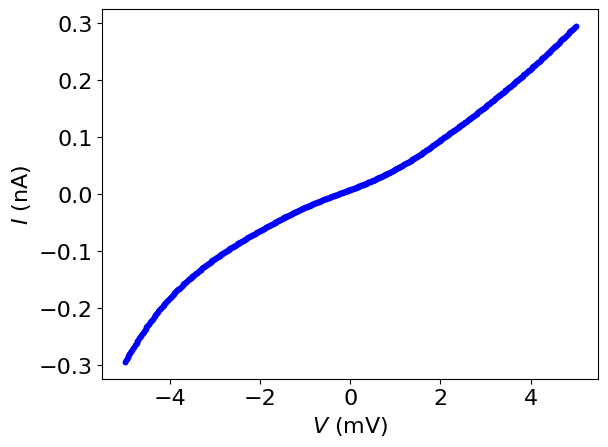
\includegraphics[width=0.49\textwidth]{IV_97.png}
         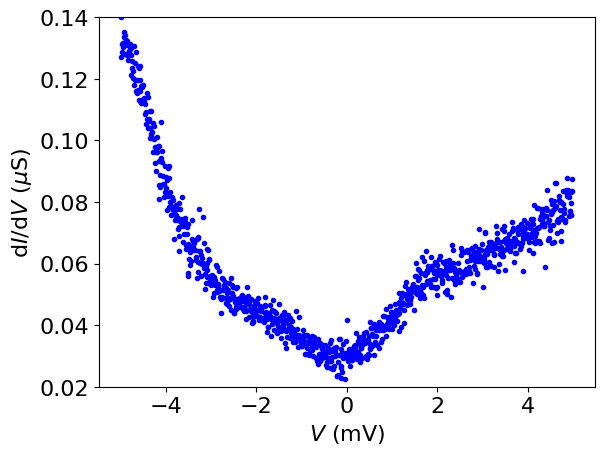
\includegraphics[width=0.49\textwidth]{dIdV_97.png}         
     \end{subfigure}
        \caption{Representative IV measurements of PdNb devices (left) and their corresponding numerical derivatives (right).}
        \label{fig:PdNb_IV}
        
\end{figure}

In figure 27, in the top left panel, it can be seen that there are two stable levels that the current fluctuates between. As a result, the differential conductance plot shows a lot of noise.

Both the junctions in figure \ref{fig:PdNb_IV} show a suppression in differential conductance around 0 mV, and the width of this suppression roughly is of the order of $\pm$1 mV, which is of the same order as $\Delta$, which was calculated at 0.95 meV for these devices. To investigate the origin of this suppression further, BIV measurements were performed. The result of one such measurement, corresponding to the same device as the bottom measurements in figure \ref{fig:PdNb_IV}, is shown in figure \ref{fig:PdNb_BIV}.



\begin{figure}[H]
     %These plots come from numid 2 from PdNb chip 6
     \begin{subfigure}[t]{0.49\textwidth}
         \centering
     	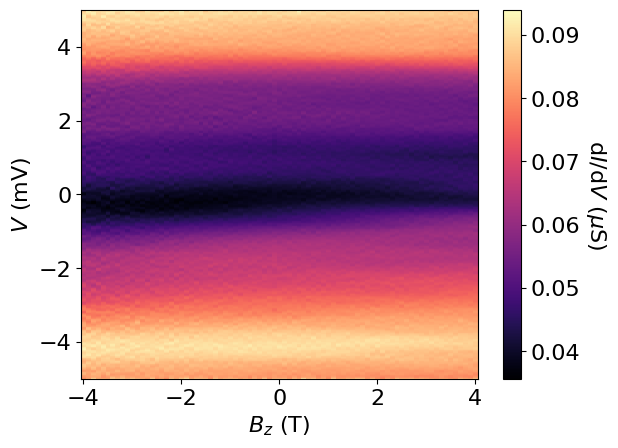
\includegraphics[width=\textwidth]{FurtherCharacterization_BdIdV_122.png}
         \caption{Representative BIV of PdNb device. }
         \label{subfig:}
     \end{subfigure}
     \hfill
     \begin{subfigure}[t]{0.49\textwidth}
         \centering
     	     	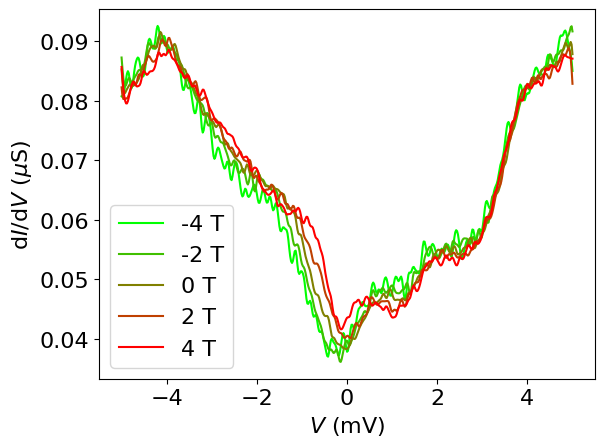
\includegraphics[width=\textwidth]{FurtherCharacterization_BdIdV_122_traces.png}
         \caption{Selected linecuts from the plot in panel (a), shown for illustration.}
         \label{subfig:}
     \end{subfigure}
        \caption{A representative BIV measurement result.}
        \label{fig:PdNb_BIV}
        
\end{figure}



The IV traces in this plot don't change significantly as a function of magnetic field. All devices were tested in this way, and none showed any clear magnetic field dependence.

\subsubsection{AuNb}

Some representative results of the IV and IVT measurements done on the AuNb devices are shown in appendix F2. Out of eleven devices, only one showed a suppression of superconductivity around zero bias that diminished at higher temperatures. Some of the measurements of this junction are highlighted here.

        
\begin{figure}[H]
     %These plots come from numid 2 from PdNb chip 6
     \begin{subfigure}[t]{\textwidth}
         \centering
         \includegraphics[width=0.49\textwidth]{/Appendix_F/F2/IV_76.png}
         \includegraphics[width=0.49\textwidth]{/Appendix_F/F2/dIdV_76.png}
         %\label{subfig:bistable_IV}
     \end{subfigure}
     \hfill
     \begin{subfigure}[t]{\textwidth}
         \centering
         \includegraphics[width=0.49\textwidth]{/Appendix_F/F2/TdIdV_183.png}
         \includegraphics[width=0.49\textwidth]{/Appendix_F/F2/TIV_183_traces.png}         
     \end{subfigure}
        \caption{Top left: IV measurement of AuNb device. Top right: numerical derivative of the IV result. Bottom left: IVT measurement of the same device. Bottom right: Selected traces from the IVT measurement.}
        \label{fig:AuNbV2_VIT}
        
\end{figure}

Figure \ref{fig:AuNbV2_VIT} does not show a clearly defined suppression in dV/dI of finite width. The IV curve remains nonlinear up to bias voltages of at least 10 mV. Furthermore, the conductivity of the device increases as a function of temperature.

\subsubsection{AuNb, 50 nm Nb}
Some representative results of the IV and BIV measurements done on the AuNb devices with 50 nm thick niobium at 30 mK are shown in appendix F3. One device is highlighted here.

\begin{figure}[H]
     %These plots come from numid 2 from PdNb chip 6
     \begin{subfigure}[t]{\textwidth}
         \centering
         \includegraphics[width=0.49\textwidth]{/Appendix_F/F3/IV_235.png}
         \includegraphics[width=0.49\textwidth]{/Appendix_F/F3/dIdV_235.png}
         %\label{subfig:bistable_IV}
     \end{subfigure}
     \hfill
     \begin{subfigure}[t]{\textwidth}
         \centering
         \includegraphics[width=0.49\textwidth]{/Appendix_F/F3/TdIdV_235.png}
         \includegraphics[width=0.49\textwidth]{/Appendix_F/F3/TdIdV_235_traces.png}         
     \end{subfigure}
     \hfill
     \begin{subfigure}[t]{\textwidth}
         \centering
         \includegraphics[width=0.49\textwidth]{/Appendix_F/F3/TdIdV_238.png}
     \end{subfigure}
        \caption{IV measurement and its numerical derivative for an AuNb device with 50 nm niobium at 30 mK after electromigration (top). The three plots on the bottom show the results of BIV measurements done on the same device at the same temperature.}
        \label{fig:AuNb_VI}
        
\end{figure}


In figure \ref{fig:AuNb_VI} we see a nonlinear IV response at low bias. The differential conductance shows suppression and peaks. The suppression is at 0 bias voltage, and the peaks are at 0.1 mV. Both the peaks and the dip are suppressed at higher magnetic field.
Out of 4 measured devices, 2 had low bias behavior similar to the one shown above.

\subsubsection{AuNb, 60 nm Spacing}
Of the AuNb devices with 60 nm bridge spacing, 4 were migrated. The differential conductances of all of these devices have a dip at zero bias voltage in between two peaks, which are at bias voltages between 0.4 and 0.9 mV. In the plot on the bottom and the plot in the top left, there a clear shoulders visible inside the conductance dip, located at approximately half the bias voltage of the peaks.

\begin{figure}[H]
     %These plots come from numid 2 from PdNb chip 6
     \begin{subfigure}[t]{\textwidth}
         \centering
         \includegraphics[width=0.47\textwidth]{/Appendix_F/F4/dIdV_70.png}
         \includegraphics[width=0.52\textwidth]{/Appendix_F/F4/dIdV_99.png}
         %\label{subfig:bistable_IV}
     \end{subfigure}
     \hfill
     \begin{subfigure}[t]{\textwidth}
         \centering
         \includegraphics[width=0.49\textwidth]{/Appendix_F/F4/dIdV_106.png}
     \end{subfigure}
        \caption{Numerical derivatives of IV measurements for AuNb devices with 60 nm bridge spacing, taken at 25 mK after electromigration.}
        \label{fig:AuNb_VI}
        
\end{figure}


\subsection{Asymmetric Critical Current}

While doing transport measurements, it was discovered that the devices show an asymmetric critical current when a magnetic field is applied, i.e. the critical current becomes dependent on the current direction. The degree to which the critical current becomes asymmetric is highly dependent on the direction of the applied magnetic field. Figure \ref{fig:PdNb_phi_theta} shows the results of $\phi$- and $\theta$-sweeps that were performed on a PdNb device before electromigration.  

\begin{figure}[H]
     \centering
     \begin{subfigure}[b]{\textwidth}
         \centering
         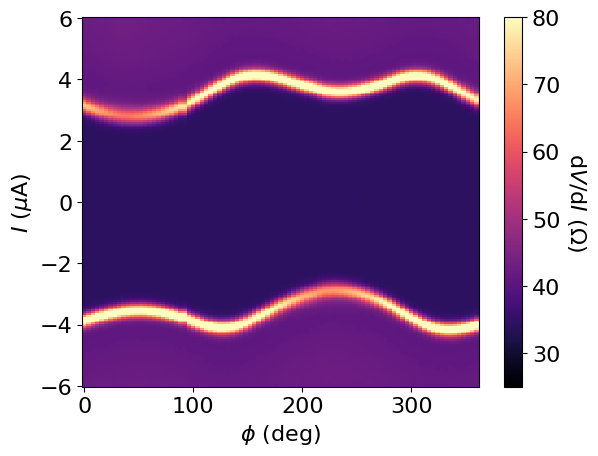
\includegraphics[width=0.49\textwidth]{dVdIphisweep_49.png}
         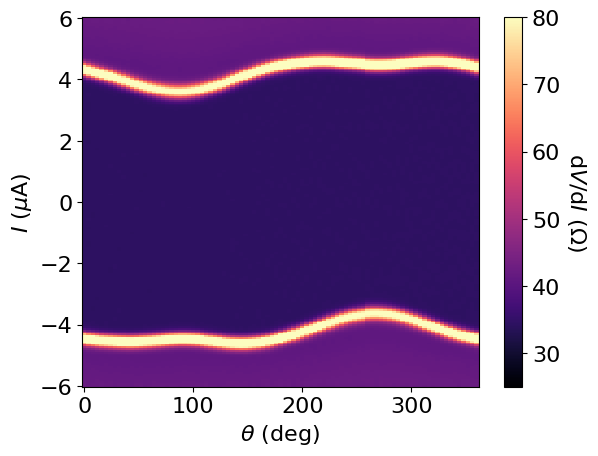
\includegraphics[width=0.49\textwidth]{dVdIthetasweep_55.png}
         %\caption{A portion of the resist is irradiated with an electron beam in as specified pattern.}
         %\label{c}
     \end{subfigure}
     \hfill
     \begin{subfigure}[b]{\textwidth}
         \centering
         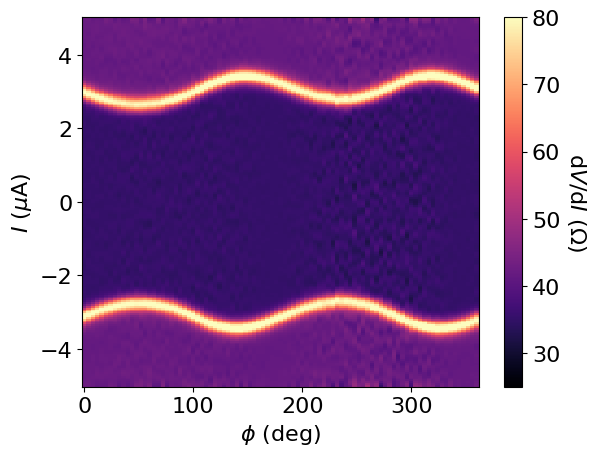
\includegraphics[width=0.49\textwidth]{dVdIphisweep_68.png}
         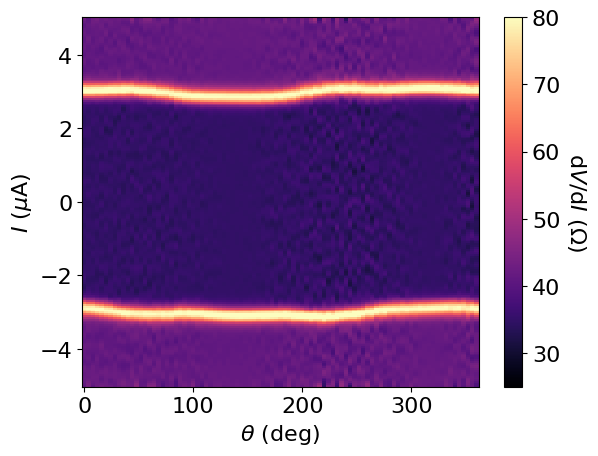
\includegraphics[width=0.49\textwidth]{dVdIthetasweep_71.png}
         %\caption{A portion of the resist is irradiated with an electron beam in as specified pattern.}
         %\label{c}
     \end{subfigure}
     \hfill
     \begin{subfigure}[b]{\textwidth}
         \centering
         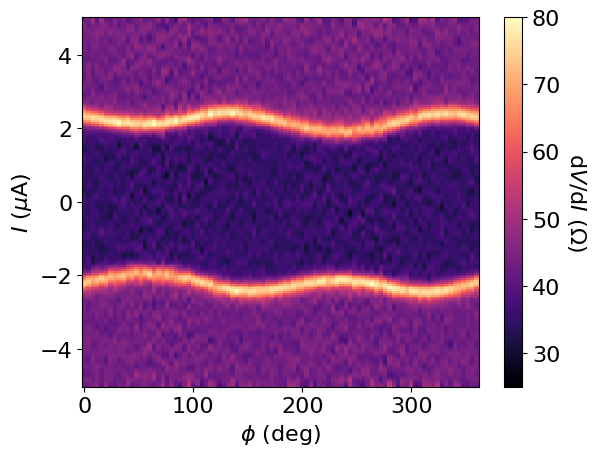
\includegraphics[width=0.49\textwidth]{dVdIphisweep_69.png}
         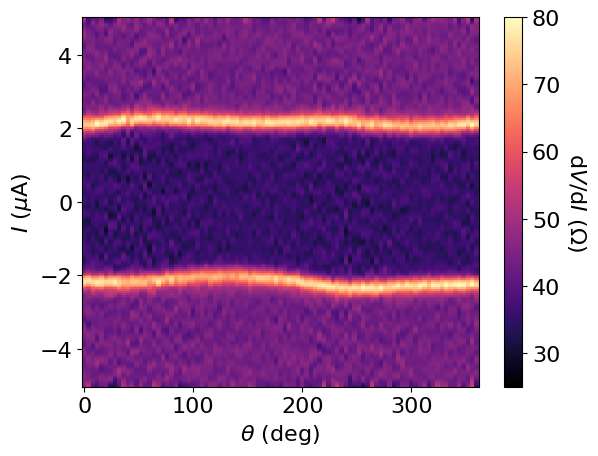
\includegraphics[width=0.49\textwidth]{dVdIthetasweep_72.png}
         %\caption{A portion of the resist is irradiated with an electron beam in as specified pattern.}
         %\label{subfig:}
     \end{subfigure}
        \caption{$\phi$ and $\theta$ sweep measurements, taken at 0.2 T. The adjacent $\phi$ and $\theta$ sweeps correspond to the same device in each case.}
        \label{fig:PdNb_phi_theta}
        
\end{figure}


Looking at the plots in figure \ref{fig:PdNb_phi_theta}, we see two bright lines where the differential resistance peaks sharply. These are the critical currents of the devices. Looking at the critical current in the positive and negative current bias directions, we see that they are not symmetric around 0 current bias.  From these measurements it can be seen that the asymmetry is strongest when the magnetic field is directed in the direction perpendicular to the junction, in plane with the devices. In these plots, this does not correspond to 90$^\circ$ and 270$^\circ$ exactly since, as discussed in the methods section, the devices are rotated slightly with respect to the axes of the magnet. For many devices, BVI measurements were performed in the directions parallel to the junction, perpendicular to the junctions in plane, and perpendicular to the junction out of plane. Many of the results from these measurements can be found in appendix D. This section will highlight only the result of selected measurements which investigate the way in which the asymmetry evolves as the junctions become more constricted and eventually broken during the electromigration process. 

A set of devices with the AuNb design with 50 nm thick niobium and a bridge spacing of 60 nm was investigated in the dilution fridge. The devices were cooled down to 25 mK, and the orientation of the devices with respect to the X Y and Z axes of the magnets was determined using a $\phi$ sweep measurement. A selected set of devices was characterized using BVI measurements in different directions, and then electromigrated using feedback controlled electromigration until the resistance had increased by a target amount. The junction was then recharacterized at this new resistance. This process was iterated. The resistance was iterated in steps ranging between a few hundred $\Omega$ and one or several k$\Omega$, until it was close to the quantum point contact (QPC) resistance, which is 12.9 k$\Omega$. At that point the resistance was increased more to the order of tens of k$\Omega$, in which regime the junction is fully broken. The results that are shown in this section show the directional magnetic field dependence of devices before any breaking was done, at the QPC resistance, and in the fully broken state. The results that will be highlighted for each of those resistance regimes are from BVI measurements in the direction parallel to the current, $B_{//}$, the direction perpendicular to the current in plane with the device, $B_{\perp}$, and the out of plane direction, $B_Z$. 



In these results, the critical current in both positive and negative direction can easily be extracted by taking the argmax of the differential conductance as a function of current for the VI trace at each temperature. Figure \ref{fig:asymetry_extraction_illustration} shows the procedure. 

\begin{figure}[H]
     %These plots come from numid 2 from PdNb chip 6
     \begin{subfigure}[t]{\textwidth}
         \centering
        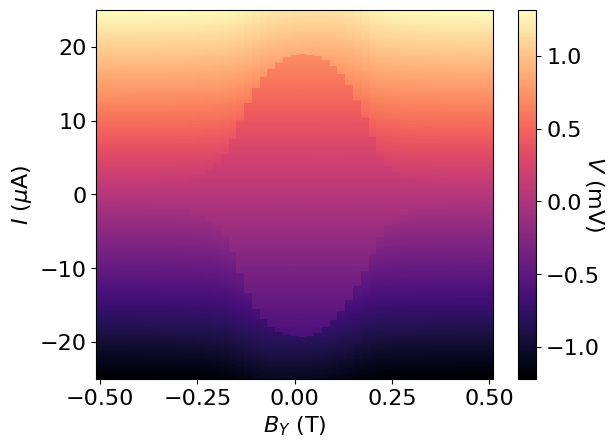
\includegraphics[width=0.49\textwidth]{IcAsymmetryExtraction00Y_42.png}
        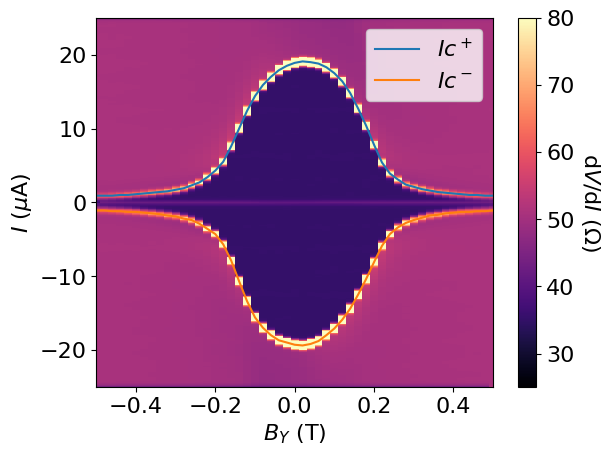
\includegraphics[width=0.49\textwidth]{IcAsymmetryExtraction0Y_42.png}
         %\label{subfig:bistable_IV}
     \end{subfigure}
     \hfill
     \begin{subfigure}[t]{\textwidth}
         \centering
        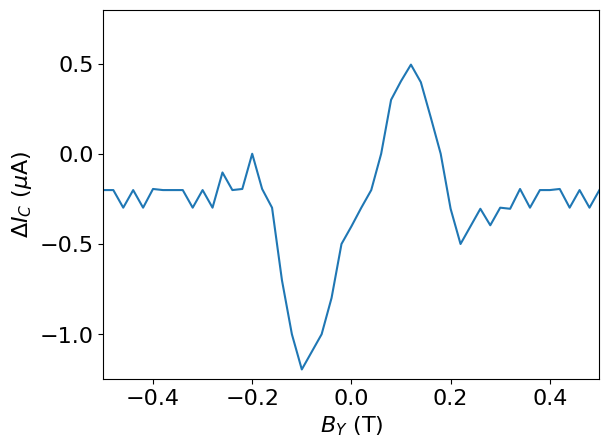
\includegraphics[width=0.49\textwidth]{IcAsymmetryExtractionY_42.png}
     \end{subfigure}
        \caption{The extraction of $\Delta I_C$. We start by determining $I_C^+$ and $I_C^-$, which we find by taking the argmax of the differential conductance for the IV traces at each magnetic field in the domain of positive and negative bias current, respectively, which is illustrated in the figure on the top right. We then take the difference in the absolute values of these two quantities to arrive at $\Delta I_C$, which is shown on the bottom.}
        \label{fig:asymetry_extraction_illustration}
        
\end{figure}

The asymmetry has been calculated for each of the magnetic field directions in this way, and the results are plotted in figure \ref{fig:BIV_SNS}.


\begin{figure}[H]
     %These plots come from numid 2 from PdNb chip 6
     \begin{subfigure}[t]{\textwidth}
         \centering
        \includegraphics[width=0.49\textwidth]{/Appendix_G/dVdIBZ_20.png}
        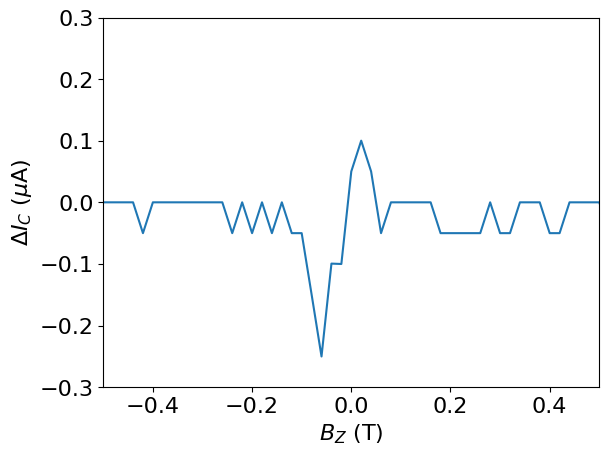
\includegraphics[width=0.49\textwidth]{IcAsymmetryExtraction_20.png}
         %\label{subfig:bistable_IV}
     \end{subfigure}
     \hfill
     \begin{subfigure}[t]{\textwidth}
         \centering
        \includegraphics[width=0.49\textwidth]{/Appendix_G/dVdIBZ_27.png}
        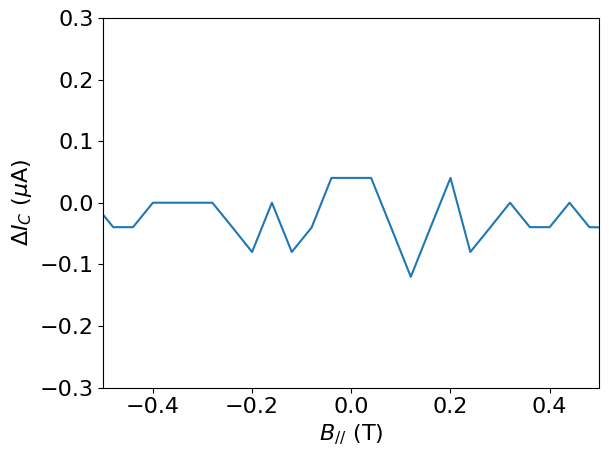
\includegraphics[width=0.49\textwidth]{IcAsymmetryExtraction_27.png}
     \end{subfigure}
     \hfill
     \begin{subfigure}[t]{\textwidth}
         \centering
        \includegraphics[width=0.49\textwidth]{/Appendix_G/dVdIBZ_25.png}
        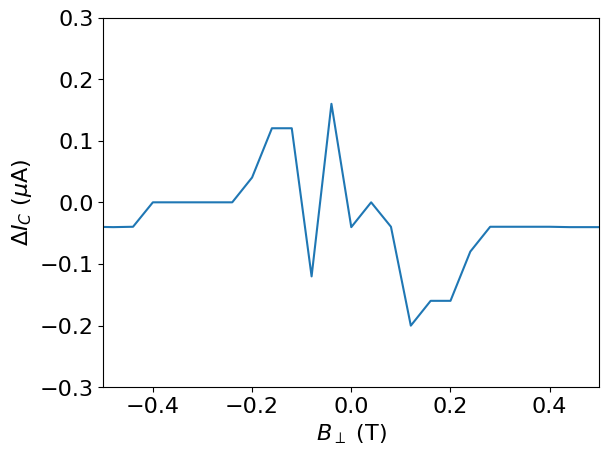
\includegraphics[width=0.49\textwidth]{IcAsymmetryExtraction_25.png}

     \end{subfigure}
        \caption{BVI measurements done on an AuNb device with 60 nm bridge spacing before electromigration. The direction of the magnetic field is in the out of plane direction (top), in the direction of the current through the device (middle), and in the direction perpendicular to the current in plane with the device (bottom), together with selected linecuts for illustration.}
        \label{fig:BIV_SNS}
        
\end{figure}

Looking at figure \ref{fig:BIV_SNS}, we see that $\Delta I_C$ is largest in the $B_{\perp}$ and $B_Z$ directions, and that the characteristic magnetic field scale over which there is a significant asymmetry is approximately 0.2 T.




\begin{figure}[H]
     %These plots come from numid 2 from PdNb chip 6
     \begin{subfigure}[t]{\textwidth}
         \centering
        \includegraphics[width=0.49\textwidth]{/Appendix_G/dVdIBZ_131.png}
        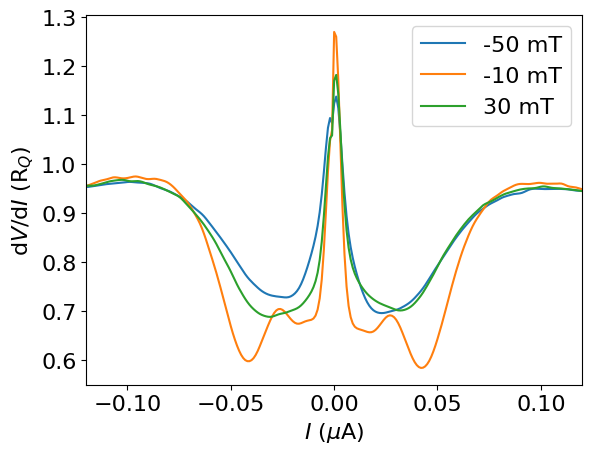
\includegraphics[width=0.49\textwidth]{IcAsymmetryExtraction_131.png}
         %\label{subfig:bistable_IV}
     \end{subfigure}
     \hfill
     \begin{subfigure}[t]{\textwidth}
         \centering
        \includegraphics[width=0.49\textwidth]{/Appendix_G/dVdIBZ_126.png}
        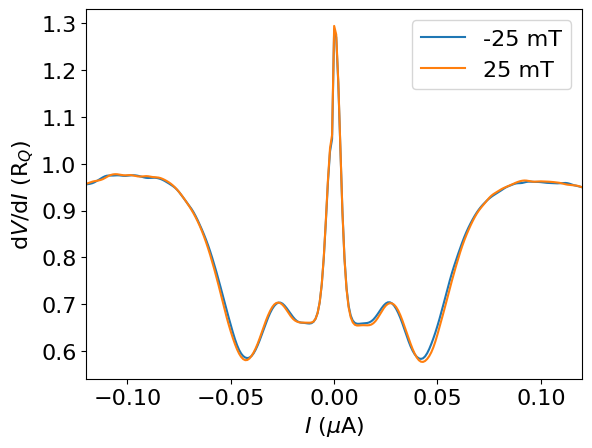
\includegraphics[width=0.49\textwidth]{IcAsymmetryExtraction_126.png}
         %\label{subfig:bistable_IV}
     \end{subfigure}
     \hfill
     \begin{subfigure}[t]{\textwidth}
         \centering
        \includegraphics[width=0.49\textwidth]{/Appendix_G/dVdIBZ_125.png}
        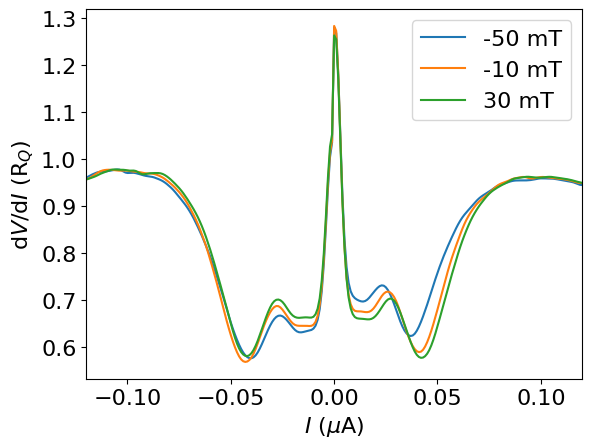
\includegraphics[width=0.49\textwidth]{IcAsymmetryExtraction_125.png}

     \end{subfigure}
        \caption{BVI measurements done on an AuNb device with 60 nm bridge spacing after electromigrating until the QPC resistance regime. The direction of the magnetic field is in the out of plane direction (top), in the direction of the current through the device (middle), and in the direction perpendicular to the current in plane with the device (bottom), together with selected linecuts for illustration.}
        \label{fig:BIV_QPC}
        
\end{figure}

In figure \ref{fig:BIV_QPC} the asymmetry in critical current is strongest in the $B_{\perp}$ direction, less strong but still visible in the $B_Z$ direction, and not discernible in the $B_{//}$ direction.

\begin{figure}[H]
     %These plots come from numid 2 from PdNb chip 6
     \begin{subfigure}[t]{\textwidth}
         \centering
        \includegraphics[width=0.49\textwidth]{/Appendix_G/TdIdV2_137.png}
        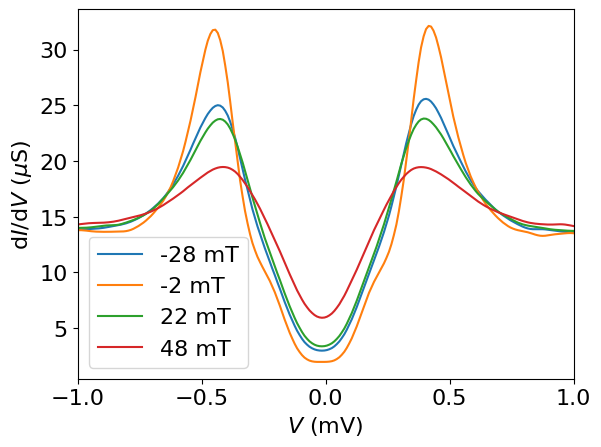
\includegraphics[width=0.49\textwidth]{IcAsymmetryExtraction_137.png}
         %\label{subfig:bistable_IV}
     \end{subfigure}
     \hfill
     \begin{subfigure}[t]{\textwidth}
         \centering
        \includegraphics[width=0.49\textwidth]{/Appendix_G/TdIdV2_134.png}
        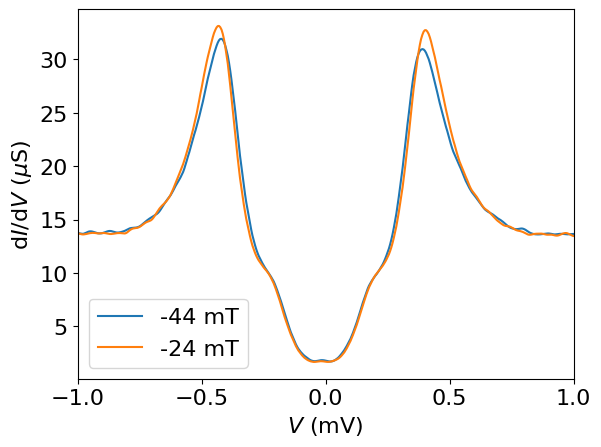
\includegraphics[width=0.49\textwidth]{IcAsymmetryExtraction_134.png}
         %\label{subfig:bistable_IV}
     \end{subfigure}
     \hfill
     \begin{subfigure}[t]{\textwidth}
         \centering
        \includegraphics[width=0.49\textwidth]{/Appendix_G/TdIdV2_133.png}
        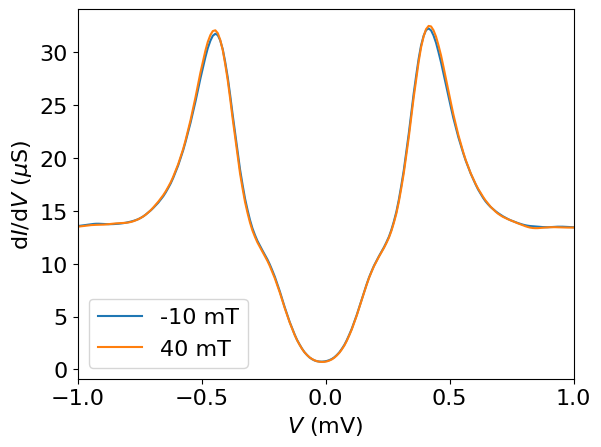
\includegraphics[width=0.49\textwidth]{IcAsymmetryExtraction_133.png}

     \end{subfigure}
        \caption{BVI measurements done on an AuNb device with 60 nm bridge spacing after electromigrating until the fully broken regime. The direction of the magnetic field is in the out of plane direction (top), in the direction of the current through the device (bottom), and in the direction perpendicular to the current in plane with the device (middle), together with selected linecuts for illustration.}
        \label{fig:BIV_SNINS}
        
\end{figure}


In figure \ref{fig:BIV_SNINS}, the only magnetic field direction along which we see obvious asymmetry in the critical current is the $B_{\perp}$ direction.








\section{Discussion}
\label{section:Discussion}

\iffalse
In this section, we discuss the results of the measurements and the SEM images that were presented in the preceding chapter. Our goal during this discussion is to provide an analysis of the results that allows us to assess the quality of our devices in terms of the 

In this chapter, we analyze the results presented in the previous chapter. Our goal is to extract relevant and information regarding the quality of the fabrication as well as the quality of the devices, which we quantify by extracting several superconducting parameters from the data. Specifically, in section 5.1 we examine the fabrication results by looking at the SEM images of the devices to determine how closely the devices match the intended design. We analyse fabrication errors and the effects of the changes that were made to the design and fabrication methods. In section 5.2, we look at the temperature dependence measurements from section 4.3 of the results in order to analyse the strength of the proximity effect, which we quantify by extracting critical temperatures and the sizes of the induced energy gaps.
\fi

\subsection{Fabrication}
\subsubsection{Niobium Layer}
As can be seen in figures \ref{fig:PdNb_fabrication_SEM} and \ref{fig:AuNb_SEM}, the devices fabricated with niobium layers of 100 nm thickness are not as intended. In those images it can be seen that niobium has ended up underneath the undercut, despite being evaporated at a straight angle. In each of the imaged devices, the niobium layer covers more of the bridge than intended, and in a portion of the devices the bridge is covered completely. In the bilayer region of the device, this discrepancy between the device design and the actual device is unlikely to significantly affect the quality of the device. At the bridge, however, this fabrication error has a large effect on the quality of the device.

There are several ways in which the unintended and inconsistent placement of niobium on the bridge affects the quality of the device. First of all, if the goal is to contact a nanoscopic object with contacts made from the chosen bridge material, the contacts that are formed after the device has been electromigrated need to be made of this material. If niobium is present at or close to the electromigration site, an alloy of niobium and the bridge material may form during electromigration and the contacts that are formed will be of this alloy instead of their intended material, and the resulting device will not have the intended properties, i.e. it will have different contact resistance with the objects that it is intended to contact, and the increased scattering caused by the mixture of materials will reduce superconductivity since the Thouless energy scales with the square root of the diffusion coefficient. 

Secondly, the inconsistency of the placement of niobium on the bridge means that experiments done using these devices will be less reproducible and the experimental conditions will be less controlled.


The presence of niobium in the undercut was hypothesized to be due to film stress in the niobium. The solution that was tried was to reduce the thickness of the niobium layer to 50 nm and to increase the rate of evaporation to 0.5 nm/s. As can be seen in figures \ref{fig:AuNbV3_SEM} and \ref{fig:AuNb60nm_SEM}, the devices that were made with these niobium evaporation parameters have niobium layers that closely match the shape of the patterned design, without the clear presence of niobium in the undercut, including on the bridge. The conclusion drawn from these images is that evaporating the niobium with the new parameters has resolved the issue that was present in the preceding devices. 

\iffalse
Based on the SEM images of the devices, we see that the distance between the corners of the niobium layers on opposite sides of the bridge is between 50 and 60 nm in the AuNb devices with 50 nm niobium thickness, which is in accordance with the distance of 50 nm specified in the design. In the AuNb devices with 60 nm bridge spacing, however, the shortest distance between the niobium layers is between 90 nm and 100 nm, which deviates from the design by over half the distance specified in the design pattern. A possible explanation for this deviation is that the e-beam exposure dose was not changed when the design pattern was changed from 50 nm to 60 nm. Since the regions close to the edge of the pattern on either side of the bridge recieve fewer secondary electrons from the other side of the bridge when the spacing is increased, the effective dose is reduced. If the goal is to match the distance in the design, therefore, the exposure dose needs to be increased when the patterned bridge distance is increased. However, we selected this pattern becuase on SEM images of a spacing test. In the spacing test, this was the design that minimized the overlap between the gold layers at the center of the bridge. Based on our test, the overlap was minimized wen the bridge spacing as 90 nm, which we achieved by patterning 60 nm and using the same dose as in the prior designs. The discrepancy between the patterned design and the resulting device is not problematic as long as we are aware that whenever we refer to the AuNb device with 60 nm bridge spacing, we are talking about a device with a bridge that is 90 nm in length.
\fi

\subsubsection{Bridge}
The images in figure \ref{fig:AuNbV3_SEM} show a region of higher brightness in the center of the bridge. We also see based on the rest of the image that this is the region at which the two gold layers that were evaporated at different angles overlap. Based on this reasoning, we can associate the region of increased brightness with a gold layer that is twice as thick as intended. 

The reason that a bowtie geometry is used is that electromigration is most likely to start in regions of higher local resistivity and current density. The bowtie geometry is designed to create a single point of maximal resistivity and current density at the center of the bridge, in order to make electromigration consistent and reproducible between different devices, and to ensure that the resulting device has optimal superconducting properties.

When the gold layers overlap in the center and double the local gold thickness there, this reduces the local current density and resistivity in that region. This makes electromigration less likely to take place in the center, and more likely to take place asymmetrically, near either end of the bridge.\\


In order to eliminate the region of overlap between the gold layers, the bridge spacing was increased from 50 nm to 60 nm. As can be seen in figure \ref{fig:AuNb60nm_SEM}, the devices that were made with this bridge spacing do not show a clear region of overlap. Another consequence of the new spacing is that the center of the geometry is more constricted than before. Both these changes ensure that the local resistivity and current density is maximal in the center of the bridge. 

The plot in figure \ref{fig:Migration_stats} shows that the there is less spread in the resistance values of the devices with 60 nm spacing after migration, which indicates a higher degree of control during the electromigration process. However, since the electromigration in the 60 nm devices was done cold and the electromigration in the 50 nm devices at room temperature, it is difficult to separate the effect of these two changes and it is not possible to draw strong conclusions from this data. When looking at the electromigration curves in appendix E3 and E4, we see that the critical voltage required to start the migration process is lower on average for the devices with 60 nm bridge spacing, and that the steps in the resistance of the device are smaller on average in those devices as well. Both of these differences indicate that electromigration is more controllable in the devices with 60 nm bridge spacing. 


\subsection{Transport Measurements Before Electromigration}

Since our goal is to characterize our SEMBJ devices, there are several parameters that we are interested in which quantify the superconductivity. Two of the most important parameters are the Thouless energy and the energy gap of the bilayer.

%including the electronic diffusion coefficient in the bridge, $D$, the Thouless energy $E_{Th}$, the superconducting coherence lengths in the superconductor and in the normal metal, and the superconducting energy gap in the bulk film. 

Determining these parameters in the device before electromigration can help characterize the electromigrated device, as well as the way the properties of the device are changed during the electromigration process. Since electromigration is expected to only change the structure of the device in the bridge while leaving the bulk film unaltered, we can reasonably assume that the bulk film properties, including $|\Delta|$, are not significantly altered by electromigration. Although we can not say the same thing about the Thouless energy, knowing what the value of the Thouless energy was before migration took place may give insight into the way electromigration changes the structure of the bridge.

%diffusion constant in the bridge, the thouless energy of the device and $\xi_N$, it is still valuable to know what these values were 





%The hypothesis is that the transport measurements in the devices before electromigration are useful for determining these values. Since electromigration is expect to only change the structure of the device in the bridge while leaving the bulk film unaltered, we can reasonably assume that the bulk film properties $\Delta$ and $\xi_S$ are not significantly altered by electromigration. Although we can not say the same thing about the diffusion constant in the bridge, the thouless energy of the device and $\xi_N$, it is still valuable to know what these values were before migration took place. Knowing this might give insight into the way electromigration changes the structure of the bridge. Although electromigration changes the shape of the bridge and its grain structure, which will change $D$, $E_{Th}$ and $\xi_N$, it seems unlikely that the changes will be on the order of several orders of magnitude. Therefore, the values of these quantities can also be used as rough estimates for the values after electromigration.


\subsubsection*{Device Properties Before Electromigration}

The critical voltage, $V_C = I_CR_N$, is an important quantity that quantifies the transport properties of the devices. The values of the critical current and normal state bridge resistance have been extracted from the VI measurements of the devices, as is discussed in the results. For each type of device, the $I_CR_N$ product has been calculated for each device and has been plotted as a function of $R_N$ in figure \ref{fig:IcRn_Products}. In order to quantify the degree to which the fabricated devices vary, we calculate the coefficient of variation of the $I_CR_N$ products for each device type. We also calculate the correlation coefficient between $I_CR_N$ and $R_N$. The values we get are shown in table \ref{tab:IcRn_Products}.

\begin{figure}[H]
     \centering
     \begin{subfigure}[b]{0.49\textwidth}
         \centering
         \includegraphics[width=\textwidth]{/Discussion/IcRn_PdNb.png}
         \caption{PdNb.}
         \vspace{5mm}
         %\label{a}
     \end{subfigure}
     \hfill
     \begin{subfigure}[b]{0.49\textwidth}
         \centering
         \includegraphics[width=\textwidth]{/Discussion/IcRn_AuNbV2.png}
         \caption{AuNb.}
         \vspace{5mm}
         %\label{b}
     \end{subfigure}
     \hfill
     \begin{subfigure}[b]{0.49\textwidth}
         \centering
         \includegraphics[width=\textwidth]{/Discussion/IcRn_AuNb, 50nm Nb.png}
         \caption{AuNb with 50 nm niobium.}
         %\label{c}
     \end{subfigure}
     \hfill
     \begin{subfigure}[b]{0.49\textwidth}
         \centering
         \includegraphics[width=\textwidth]{/Discussion/IcRn_AuNb, 60 nm Spacing.png}
         \caption{AuNb with 60 nm bridge spacing.}
         %\label{d}
     \end{subfigure}
        \caption{Scatter plots of the $I_CR_N$ products of the devices, as a function of $R_N$.}
        \label{fig:IcRn_Products}
        
\end{figure}

\begin{table}[H]
\caption{Coefficient of variation, defined as the ratio between the standard deviation and the mean, of the $I_CR_N$ products of the different types of devices, as well as the correlation coefficient between the $I_CR_N$ products and the normal state bridge resistances of the devices.}
\label{tab:IcRn_Products}
\begin{tabular}{|c|c|c|}
\hline 
Device & Coefficient of Variation & Correlation Coefficient \\ 
\hline 
PdNb & 65.9\% & 0.003 \\ 
\hline 
AuNb & 13.8\% & 0.99 \\ 
\hline 
AuNb, 50 nm Nb & 7.2\% & -0.64 \\ 
\hline 
AuNb, 90 nm Spacing & 27.6\% & -0.80 \\ 
\hline 
\end{tabular} 

\end{table}

The reason that we are interested in $I_CR_N$ as a function of $R_N$, is that, with minimal changes to the device design, $R_N$ could be measured at room temperature using a 4 point measurement. If there is a correlation between $I_CR_N$ and $R_N$, the $R_N$ value can then be used to select the junctions that are likely to have a high $I_CR_N$ product based on this correlation. If there is no correlation or only a very weak correlation, the junctions with the highest $R_N$ value can be chosen, since a higher value of $R_N$ improves electromigration.  The PdNb devices show the most variation in their $I_CR_N$ product. Based on the SEM images of these devices, we know that their fabrication was very inconsistent, so this is not a surprising result. The correlation coefficients don't show a pattern across devices. The $I_CR_N$ product of the PdNb device is not correlated to its normal state bridge resistance. The other devices show strong correlations, but not in a consistent direction. Further research would be needed to determine the underlying causes of these differences. Doing so would be worthwhile, especially if it would allow us to intentionally create a strong positive correlation, such as the AuNb devices show here. If that were possible, those devices could be selected based on simple room temperature measurements that have a high normal state bridge resistance as well as a high expected $I_CR_N$ product. Although we were not able to determine the mechanism which determines the correlation between $I_CR_N$ and $R_N$, this discussion does show that if the correlation coefficient of a set of devices is known, it can be usefully employed in device selection before the devices are loaded into a measurement setup and cooled. 

\subsubsection{Critical Temperature}

In the VIT measurements of the devices, such as for example figure \ref{fig:AuNbV2_VIT}, we can distinguish three distinct regions. In the region of low temperature and low current, the resistance of the device is lowest. We interpret this as the region in which the both the bridge and the bulk film are superconducting. Because the bridge has a smaller cross-section than the bulk film, the local current density is higher there than in the bulk film. Therefore, the critical current density is reached at a lower total current. Furthermore, in the devices where there is no niobium on the bridge, the bridge material is proximitized less strongly than it is in the bulk film, since the degree of proximitization decreases as the distance to the superconductor increases. Therefore, in the bridge, the critical temperature and current density are lower than in the bulk film. The critical current of the bridge can be seen in the VIT measurements as a function of temperature, as two converging lines of high differential resistance separating the region of lowest device resistance from a region of higher device resistance. The critical current in these plots decreases as a function of temperature, as expected. In this region of higher device resistance the bridge is no longer superconducting, but the bulk film still is. At higher temperature, there is a sharp transition as the temperature exceeds the critical temperature of the bulk film, and the entire device transitions to the normal state. Since the cross section of the bulk film is much larger than that of the bridge, the current range of the measurement is too small to resolve the critical current of the bulk film as a function of temperature. 

We can extract the differential resistance of the device at zero bias current from the VIT measurements. In such a plot, we can identify three regions of relatively constant resistance, separated by regions of large gradient of resistance as a function of temperature. The critical temperature is taken to be the temperature at which the resistance is halfway between the normal state resistance and the superconducting state resistance. An example of such an extraction is shown in figure \ref{fig:TC_extraction}.

\begin{figure}[H]
     %These plots come from numid 2 from PdNb chip 6
     \centering
     \begin{subfigure}[t]{0.66\textwidth}
         \centering
         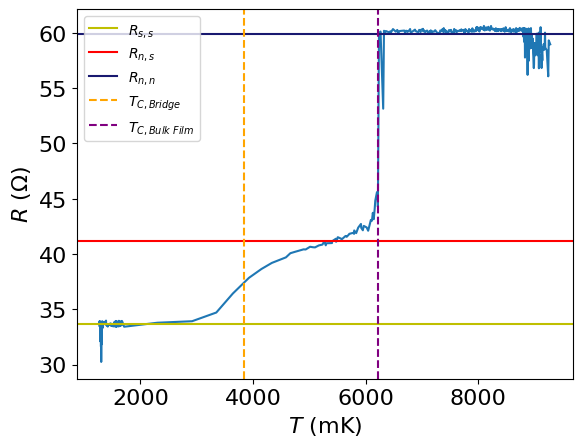
\includegraphics[width=\textwidth]{Discussion/PdNb_Rt_Tc_extraction.png}
         %\caption{Representative VIT}
         \label{subfig:}
     \end{subfigure}
     \caption{Representative graph showing the zero bias current differential resistance as a function of temperature. }
     \label{fig:TC_extraction}
        
\end{figure}

We also extract the width of the superconducting transition, $\Delta T_C = T90\% - T10\% $, where $T90\% $ and $T10\% $ are the temperatures corresponding to $90\% $ and $10\% $ of the resistivity jumps, respectively. All the extracted critical temperatures and their widths for the different devices are shown in table \ref{tab:TC_extraction}.



In order to establish a relationship between the critical temperature in the bulk film and the critical temperature in the bridge, we also show the ratio of these two temperatures in table \ref{tab:TC_extraction}. 

\begin{table}[H]
\caption{$T_C$ and $\Delta T_C$ values for the bridge and bulk film in the different devices, in mK, as well as the ratios of the bridge $T_C$ and bulk film $T_C$, the ratio of the bulk film $T_C$ and the $T_C$ of a bare niobium layer of the same thickness, and transparency as fitted using eq. \ref{eq:BilayerTc} from the theory. Bridge $T_C$ not clearly defined for the AuNb device with 50 nm Nb and 50 nm spacing.}
\label{tab:TC_extraction}
\centering
\begin{tabular}{|c|c|c|c|c|c|c|c|}
\hline 
Device & $T_{C, B}$ & $\Delta T_{C, B}$ & $T_{C, BF}$  & $\Delta T_{C, BF}$ \\ 
\hline 
PdNb & 3844 & 1669 & 6226 & 112 \\ 
\hline 
\makecell{AuNb, \\ 100 nm Nb} & 5132 & 1303 & 8853 & 1086 \\ 
\hline 
\makecell{AuNb, 50 nm Nb, \\ 50 nm Spacing} & $\approx$ 5800 & - & 8804 & 899 \\ 
\hline 
\end{tabular} 

\end{table}

Using the obtained $T_C$ value for the bulk film, we can immediately calculate the superconducting energy gap of the bulk film using the equality $\Delta = 1.764k_BT_C$. The energy gaps thus obtained  are tabulated in table \ref{tab:TC_extraction_calculations}. 


As mentioned in the chapter on theory, pure niobium films of 50 nm and 100 nm thickness have respective critical temperatures of 8.9 K and 9.1 K approximately. If we compare the bulk film critical temperatures in table \ref{tab:TC_extraction} to these values, can give us a measure of the degree to which the bilayers are (inversely) proximitized. The ratio between the bulk film critical temperature and the critical temperature of a pure niobium layer with corresponding thickness, is shown in table \ref{tab:TC_extraction_calculations}.

\iffalse
\noindent \textbf{Interface Transparency Fit}
The devices studied in this thesis can be modelled as SN-bilayer normal metal SN-bilayer junctions. The bulk film $T_C$ is the $T_C$ of the SN-bilayer. In equation \ref{eq:BilayerTc} on the critical temperature of an SN bilayer, for each device type all parameters are known except for the interface transparency $t$. This means that we can use equation \ref{eq:BilayerTc} to fit the interface transparency. One detail is of note in this procedure, namely that the films are not truely bilayers, but in fact trilayers since there is a 5 nm Ti sticking layer in each case. Looking at table \ref{tab:Bilayer_Table}, we see that the density of states at the Fermi energy is of the same order for Au and Ti, while the density of states at the Fermi energy of Pd is an order of magnitude larger. Based on this, we hypothesise that the Ti layer has negligable influence on the critical temperature in Pd-bridged devices, and we omit it in the fit. In the case of Au-brided devices, we cannot assume that the influence of the Ti layer is negligible, since Ti has a density of states at the Fermi energy that is larger than that of Au. The influence of the Ti layer on the bulk film critical temperature is reduced, however, if the interface transparency is less than one. Because the Ti layer and Au layer are evaporated in the same evaporator, and the device is kept under high vacuum in between the evaporation of the two layers, we assume that the interface transparency is less than but on the order of one. The effect Ti has on lowering the $T_C$ is also mitigated to some degree by the fact that Ti has a critical temperature that is slightly higher than zero (is that true? not sure). Based on these condsideraions, we then make the simplifying approximation that we can use the density of states at the Fermi energy for gold for the value of $n_n$ in equation \ref{eq:BilayerTc}, and simply add the thicknesses of the Ti and Au layer to arrive at $d_n$. The values found by fitting the transparency coefficient $t$ in this way are also shown in table \ref{tab:TC_extraction_calculations}.\\
\fi

\begin{table}[H]
\caption{The ratio of the bulk film $T_C$ and the $T_C$ of a bare niobium layer of the same thickness,$\frac{T_{C, B}}{T_{C,Nb}}$ as well as the ratio of the critical temperatures of the bridge and the bulk film, $\frac{T_{C, B}}{T_{C,Nb}}$ and the bilayer energy gap $\Delta_{BF}$.}
\label{tab:TC_extraction_calculations}
\centering
\begin{tabular}{|c|c|c|c|c|c|c|c|}
\hline 
Device &  $\frac{T_{C, B}}{T_{C,Nb}}$ & $\frac{T_{C, B}}{T_{C,BF}}$  & $\Delta_{BF}$\\ 
\hline 
PdNb & 67\% & 62\%  & 0.95 meV\\ 
\hline 
\makecell{AuNb, \\ 100 nm Nb} &  99.4\% & 58\%  & 1.35 meV\\ 
\hline 
\makecell{AuNb, 50 nm Nb, \\ 50 nm Spacing} & 98.9\% & 66\%  & 1.34 meV\\ 
\hline 
\end{tabular} 

\end{table}


For the AuNb devices with 60 nm bridge spacing, no VIT measurement was done. Since only the bridge design was changed, and the bulk film fabrication was identical to the AuNb devices with 50 nm niobium and 50 nm bridge spacing, we can assume that the bulk film properties of these two device types are similar. Since the bridge dimensions are changed between the two device designs, a similar extrapolation for the bridge $T_C$ is difficult, but based on the theory it seems reasonable to assume that the bridge $T_C$ is on average lower in the 60 nm bridge spacing devices, since the strength of the proximity effect decreases with distance.


In table \ref{tab:TC_extraction} we see that for all devices the ratios between the critical temperature of the bridge and the critical temperature of the bulk film are all within a few percent of 60\%. This suggests that there is a consistent relationship between the critical temperature of the bulk film and that of the bridge, and that the critical temperature of the bulk film is therefore a relevant quantity when investigating the critical temperature of the bridge. 

%\noindent \textbf{Agreement with Theory}\\
Based on table \ref{tab:TC_extraction}, we can conclude that changing the bridge material from palladium to gold led to a higher critical temperature for the device. This agrees with our expectations based on equation \ref{eq:BilayerTc}, since gold has a much lower density of states at the Fermi energy compared to niobium. 

%In fact, if we use equation \ref{eq:BilayerTc} to calculate the ratio between the critical temperatures of the two devices, assuming a transparency of 0.5 for both, we find that this ratio is 0.697. The ratio of bulk film critical temperatures in table \ref{tab:TC_extraction} is 0.712, which is in good quantative agreement with this prediction, despite the fact that the transparency as given by the fit is not constant.

Table \ref{tab:TC_extraction} also shows that the changes that were made as the device design was iterated from the AuNb design with 100 nm Nb to the AuNb design with 50 nm Nb made only a small difference in terms of the critical temperature of the bulk film.

% The graph of $T_C$ as a function of Nb thickness predicted by equation \ref{eq:BilayerTc}, using the parameters corresponding to the AuNb device with 100 nm Nb and a transparency of 0.15, is plotted in figure \ref{fig:palladium_thickness_tc_theory}. In this plot we see that at 100 nm Nb thickness the theory predicts that we are already far in the asymptotic regime, where the partial derivative of the bilayer critical temperature with respect to the thickness of the superconductor is relatively small. Quantitatively, equation \ref{eq:BilayerTc} predicts that the critical temperature is reduced by only 0.15\% when the thickness of the gold layer is increased from 26 nm to 30 nm and the thickness of the niobium is reduced from 100 nm to 50 nm, assuming that the transparency coefficient remains at 0.15.

\iffalse
\begin{figure}[H]
     %These plots come from numid 2 from PdNb chip 6
     \centering
     \begin{subfigure}[t]{0.66\textwidth}
         \centering
         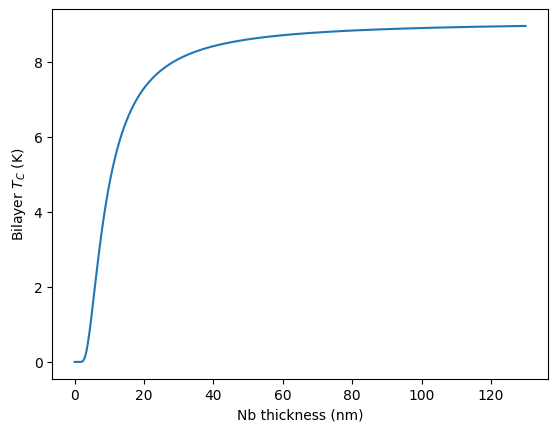
\includegraphics[width=\textwidth]{Bilayer_Tc_Theory_Graph.png}
         %\caption{Representative VIT}
         \label{subfig:}
     \end{subfigure}
     \caption{Graph showing the predicted $T_C$ value of a gold-niobium bilayer as a function of the thickness of the niobium layer. The graph assumes a transparency of 0.15 and a gold layer thickness of 26 nm. Graph based on equation \ref{eq:BilayerTc}.}
     \label{fig:palladium_thickness_tc_theory}
        
\end{figure}

\fi


%The transparency values that were fitted are shown in table \ref{tab:TC_extraction}. One thing that stands out in these data is that the interface transparency of the PdNb device is much higher than the interface transparency of both AuNb devices. A factor that likely contributes to this difference is the fact that 

The interface transparency between the bridge material and niobium layer is an important parameter that determines how well the superconducting electrons are able to enter the bridge and thereby induce superconductivity. The fact that we see induced energy gaps of the order of the energy gap of bare niobium implies that the interface transparency is sufficiently high. One aspect of fabrication that may have a particularly strong influence on the interface transparency is the exposure of the normal metal film before the evaporation of the niobium layer. Palladium and niobium are evaporated in the same evaporator, while gold and niobium are evaporated in different evaporators. This means that in the case of gold-bridged devices, the gold surface is exposed to air during the transport between the two evaporators, which may allow for contaminants to reduce the pristineness of the gold-niobium interface. The PdNb devices, on the other hand, remain in high vacuum between the evaporation of palladium and niobium and thereby minimize the amount of contamination at the interface. Since the interface transparency is an important parameter governing the quality of the superconductivity in the bridge, steps should be taken to ensure that its value is maximized. Ideally, an evaporator would be used in which both gold and niobium are available. In case that is not possible, the time in which the device is exposed to air in between the evaporation of gold and niobium should be minimized. \\

  






\iffalse
\subsubsection*{Bridge Resistance}

When looking at the IV meaurements that were done on the devices before breaking it stands out that all the devices have a near consant differential resistance around zero bias current, which then makes a sharp transition and ends up at a near constant higher resistance. As mentioned, we can interpret this as a sign of superconductivity, and associate the current of the jump with the critical current of the bridge. All the measured devices show this behavior, and so we can conclude that all the devices are superconducting before breaking. We also note that the ability to extract the normal state bridge resistance from a VI measurement is something that would be impossible in a device that does not incorporate superconductivity, which is one of the benefits SEMBJs have over normal state EMBJs. 

In order to estimate the effective length of the bridge, and to validate the normal state bridge resistances in our results, we estimate the normal state bridge resistance of the AuNb device with 50 nm niobium using a SEM image of the device before breaking and the literature values for the resistivity of thin gold films. 

Looking at the SEM image of the AuNb device with 50 nm niobium, we estimate the bridge to be the region of gold film in between the corners of the niobium layer. This region is next approximated with three rectangles, as is shown in figure \ref{fig:BridgeResistanceExtraction}. Based on the discussion on the fabrication results, we know that the thickness of the gold film in the yellow regions is 15 nm, while in the orange region it is 30 nm. We can estimate the height and width of the rectangles using the scale bar of the SEM image. Using the literature values of the resistivity of 15 nm and 30 nm thick gold films (191 $\Omega$nm and 40 $\Omega$nm respectively), we can then calculate the total resistance of the three rectangles, which we model as three resistances in series. The result of this calculation is a resistance of 6.1 $\Omega$. As can be seen in figure \ref{fig:AuNbV3_VI}, the values for the normal state bridge resistance that were extracted from the measurements for these devices are all in the range of 5 to 6 $\Omega$. Therefore we can conclude that the effective length of the junction is close to its geometric length of 50 nm, and that the results of the VI measurements, and our interpretation of those results, are reasonable.


\begin{figure}[H]
     %These plots come from numid 2 from PdNb chip 6
     \centering
     \begin{subfigure}[t]{0.66\textwidth}
         \centering
         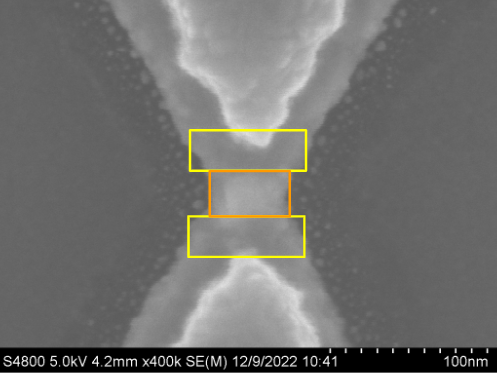
\includegraphics[width=\textwidth]{BridgeREstimate.png}
         %\caption{Representative VIT}
         \label{subfig:}
     \end{subfigure}
     \caption{Graph showing the predicted $T_C$ value of a gold-niobium bilayer as a function of the thickness of the niobium layer. The graph assumes a transparency of 0.15 and a gold layer thickness of 26 nm. Graph based on equation \ref{eq:BilayerTc}.}
     \label{fig:BridgeResistanceExtraction}
        
\end{figure}
\fi


 




\subsubsection{Thouless Energy}

Using equations \ref{eq:E_Th(D,L)} and \ref{eq:Xi_N_of_T}, we can express the Thouless energy purely as a function of the ratio $L/\xi_N(T_C)$ and $T_C$: 

$$E_{Th}\left(\frac{L}{\xi_N(T_C)}\right) = 2\pi k_BT_C / \left(\frac{L}{\xi_N(T_C)}\right)^2$$

Since $T_C$ is known for the devices, we can get the ratio $L/\xi_N(T_C)$ from figure \ref{fig:V_C_of_T_for_different_L_over_Xi} and the critical voltage of the devices as a function of temperature. 


In order to determine $V_C(T)$, we need $I_C(T)$ and $R_N$. The critical current can be extracted as a function of temperature from a VIT measurement simply by taking the argmax of the differential resistance as a function of current at each temperature. The result of such an extraction is plotted in figure \ref{fig:IcExtraction} for the IVT plot from figure \ref{fig:AuNbV2_VIT} from the results. 

\begin{figure}[H]
     %These plots come from numid 2 from PdNb chip 6
     \centering
     \begin{subfigure}[t]{0.66\textwidth}
         \centering
         \includegraphics[width=\textwidth]{/Discussion/IcExtraction.png}
         %\caption{Representative VIT}
         \label{subfig:}
     \end{subfigure}
     \caption{Illustration of the extraction of $I_C$ as a function of temperature from a VIT measurement.}
     \label{fig:IcExtraction}
        
\end{figure}

Since $R_N$ has been determined for each device, we can obtain $V_C = I_CR_N(T)$ by multiplying $I_C(T)$ with $R_N$. We can then rescale the temperature and $V_C$ in the same way as they are scaled in figure \ref{fig:V_C_of_T_for_different_L_over_Xi}, such that we can compare our devices with that plot. The extracted values of $I_CR_N$ have been plotted for each device for which a VIT measurement was done, and the lines from figure \ref{fig:V_C_of_T_for_different_L_over_Xi} have been reproduced in order to facilitate comparison. The result is shown in figure \ref{fig:likharev_plot}. We can use this plot to extract the ratio $\xi_N(T_C) / L$. We can also gauge the degree to which our measurements are described by the theory, by how well the temperature dependence of the $I_CR_N$ products follows the shapes of the curves in figure \ref{fig:V_C_of_T_for_different_L_over_Xi}. We see that the curves closely follow the shape of the curves from the theory, indicating the validity. In the case of the AuNb devices with 60 nm bridge spacing, no VIT measurement was done, and for this device the average of all $I_CR_N$ values, which were all obtained at the same temperature, is used. 

\begin{figure}[H]
     %These plots come from numid 2 from PdNb chip 6
     \centering
     \begin{subfigure}[t]{0.66\textwidth}
         \centering
         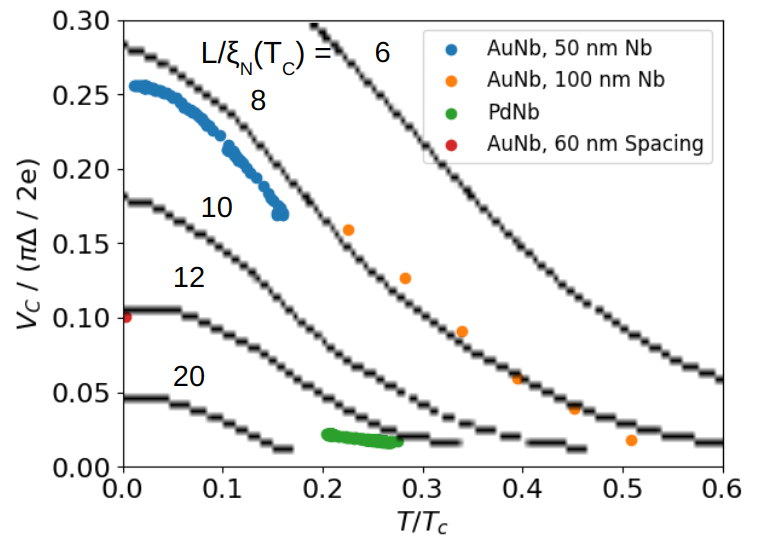
\includegraphics[width=\textwidth]{Likharev_plot_all4.png}
         %\caption{Representative VIT}
         \label{subfig:}
     \end{subfigure}
     \caption{Comparison of $I_CR_N(T)$ with the theoretical result extracted from figure \ref{fig:V_C_of_T_for_different_L_over_Xi}.}
     \label{fig:likharev_plot}
        
\end{figure}

From this figure, we can estimate the ratio $L/\xi_N$ to be approximately 8 for the AuNb device, 12 for the average AuNb device with 60 nm spacing, 8.5 for the AuNb device with 50 nm niobium, and somewhere between 12 and 20 for the PdNb devices. For the PdNb device the estimation is more difficult, but we will choose 14 for our estimate. Finally, we find the Thouless energies by substituting these values into the equation above. The obtained values are shown in table \ref{tab:E_Th_SNS}.

\begin{table}[H]
\caption{Thouless energy calculated using the $L/\xi_N(T_C)$ value obtained above for each device type.}
\label{tab:E_Th_SNS}
\centering
\begin{tabular}{|c|c|c|c|c|c|}
\hline 
Device &  $E_{Th}$ ($\mu$eV)\\ 
\hline 
PdNb & 18  \\ 
\hline 
AuNb &  75 \\ 
\hline 
AuNb, 50 nm Nb & 67  \\ 
\hline 
AuNb, 60 nm Spacing & 33   \\ 
\hline 
\end{tabular} 

\end{table}

\iffalse
\subsection*{$\xi_N, D, l$ and $L$}

The devices can be further characterized by determining the superconducting coherence length, diffusion coefficient, mean free path and effective device length. Since we know the thouless energies of the devices, we only require one of these parameters to determine all the others, using formulas \ref{eq:E_Th(D,L)}, \ref{eq:Xi_N_of_T} and $D = v_f*l/3$. We will estimate the mean free path using the literature values of the film resistances corresponding to our bridge materials. Since the bridges are constricted films and not bulk films, this estimate is likely to overestimate the actual mean free path length, since the constriction in the film causes additional surface scattering. We use the following relationships between the resistivity and mean free path of palladium and gold: for palladium $rho*l = $
\fi

\iffalse
Using the relationship $l*\rho$ = 835 $\Omega$nm$^2$ \cite{Electron mean free path in elemental metals} and the resistivities of 13 nm and 15 nm thick gold layers (2.28 $\Omega\mu$m and 190 $\Omega$nm, respectively \cite{Electrical resistivity of gold thin film as a function of film
thickness}) we can obtain a rough estimate of $l$ in the gold bridged devices. Since the gold layers are constricted, the added boundary scattering caused by the constriction relative to a bulk film means that we expect this estimate of $l$ to be too high. 

\begin{table}[H]
\caption{}
\label{tab:likharev_table}
\centering
\begin{tabular}{|c|c|c|c|c|c|}
\hline 
Device & $L$ (nm) & $\xi_N(T_C)$ (nm) & $D$ (cm$^2$/s) & $E_{Th}$ ($\mu$eV) & $l$ (nm) \\ 
\hline 
PdNb & & 3.6 & 0.66 & 17.5 & 0.20 \\ 
\hline 
AuNb & 38.4 & 4.8 & 1.7 & 75.2 & 0.37 \\ 
\hline 
AuNb, 50 nm Nb & 141 & 16.7 & 20.1 & 66.7 & 4.37 \\ 

\hline 
\end{tabular} 

\end{table}

----------------\\
We know that for the AuNb devices with 50 nm niobium, the gap sizes are consistently close to 50 nm. For the PdNb devices and the AuNb devices with 100 nm niobium, however, we know that the bridge length is often lower than intended in the design. We will still take $L$ to be 50 nm in those devices, and keep in mind that this is an imprecise estimate for these devices.

Looking at figure \ref{fig:likharev_plot}, we see that the shape of the $I_CR_N$ curves of our devices match the shapes of the theoretical figure. The AuNb device with 50 nm niobium matches the shape most closely, and for the PdNb device the degree of agreement is most difficult to estimate, due to the small temperature range and low value of its critical voltage.

From this figure, we can estimate the ratio $L/\xi_N$ to be approximately 8 for the AuNb device, 8.5 for the AuNb device with 50 nm niobium, and somewhere between 12 and 20 for the PdNb devices. For the PdNb devise the estimation is more difficult, but we will choose 14 for our estimate. These ratio's allow us to calculate $\xi_N(T_C)$. The values obtained for $\xi_N(T_C)$ in this way are 5.9 nm for the AuNb device with 50 nm niobium, 6.3 nm for the AuNb device with 100 nm niobium, and 3.6 for the PdNb device. These values have been tabbulated in table \ref{tab:likharev_table}.

Usign equation \ref{eq:Xi_N_of_T}, we can then find the value of $D$, the normal metal diffusion constant. In turn, we can use $E_{Th} = D\hbar/L^2$ and $D = v_Fl/3$ to calculate the Thouless energy and electron mean free path in the bridge. All the calculated values are shown in table \ref{tab:likharev_table}.

-----------------

\begin{table}[H]
\caption{}
\label{tab:likharev_table}
\centering
\begin{tabular}{|c|c|c|c|c|}
\hline 
Device & $\xi_N(T_C)$ (nm) & $D$ (cm$^2$/s) & $E_{Th}$ ($\mu$eV) & $l$ (nm) \\ 
\hline 
PdNb & 3.6 & 0.66 & 17.5 & 0.20 \\ 
\hline 
AuNb & 6.3 & 2.89 & 76.1 & 0.62 \\ 
\hline 
AuNb, 50 nm Nb & 5.9 & 2.52 & 66.3 & 0.54 \\ 
\hline 
AuNb, 60 nm Spacing & 3.8 & 1.04 & 19.0 $\pm$ 4.9 & 0.31 \\ 
\hline 
\end{tabular} 

\end{table}

Discussion of the table.


\noindent A second method for calculating these quantities is using formulas \ref{eq:IcRn_at_low_T} and \ref{eq:generalized_thouless_energy}, relating the critical voltage and Thouless energy at zero and finite temperature, respectively. In figure \ref{fig:AuNbV3DF_VIT} we see that at 30 mK, the critical current has saturated. This means that at 30 mK we can use the zero temperature limit in our calculation of $E_{Th}$. For the junctions measured at higher temperatures, we use equation \ref{eq:generalized_thouless_energy} to fit the thouless energy.

The $I_C$ and $R_N$ values in figure \ref{fig:AuNb60nm_VI}b for the AuNb devices with 60 nm bridge spacing were all extracted from VI measurements that were done at 25 mK. Applying equation \ref{eq:generalized_thouless_energy} to these values gives a Thouless energy of 19.0 $\pm$ 4.9 $\mu$eV.


---------
 \fi

\subsection{Transport Measurements After Electromigration}

In order to characterize the superconductivity of the broken junctions, we are looking for features which are characteristic of superconductivity in the transport measurements. In a broken junction, superconductivity manifests itself as a suppression of the differential conductivity around zero bias. The width of the suppression should be on the order of $\mathrm{min}(E_\mathrm{Th}, \Delta)$. The suppression should also be lifted when superconductivity ceases, for example when the temperature or magnetic field exceed the critical temperature or critical field. Other mechanisms might suppress conductivity at zero bias, such as a tunnel barrier or a SET for example. If no suppression is seen, that means either that the junction is not superconducting, or that the gap is too small to be resolved. In either case, the junction is not a useful SEMBJ. 
Superconductivity may also manifest itself as a peak in differential conductance as a result of Andreev reflections. 
After electromigration, the PdNb and AuNb devices showed no clear sign of superconductivity at 1.2 K and 1.9 K respectively. The results shown in figure \ref{fig:AuNbV2_VIT} do show a reduced conductivity around zero bias that is diminished at higher temperatures, but it is not obvious whether this measurement indicates superconductivity. If this feature is indicative of superconductivity, the superconductivity is not of sufficient quality for the junction to be used as an SEMBJ.  The AuNb with 50 nm niobium and those with 60 nm bridge spacing did show superconducting features in measurements done at 30 mK and 25 mK respectively.

We can identify coherence peaks in the differential conductance plots of the electromigrated AuNb devices with 50 nm niobium and the devices with 60 nm bridge spacing. We can extract the voltages corresponding to these peaks from the plots, as is illustrated in figure \ref{fig:Vc_Extraction}. 

\begin{figure}[H]
     %These plots come from numid 2 from PdNb chip 6
     \centering
     \begin{subfigure}[t]{0.49\textwidth}
         \centering
         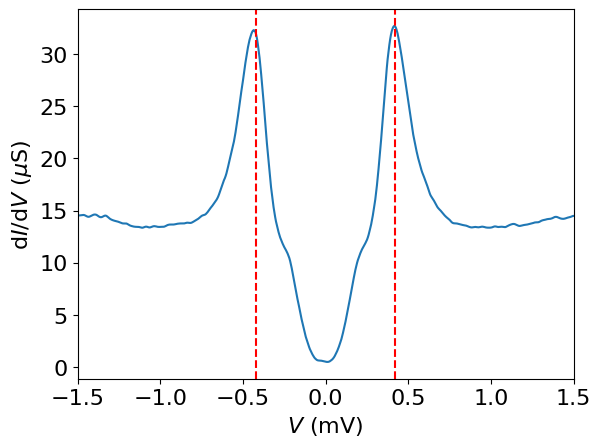
\includegraphics[width=\textwidth]{Discussion/AuNb60nm_VcExtraction.png}
         \caption{Differential conductance of AuNb device with 60 nm bridge spacing, measured at 25 mK, with the extracted $V_C$ values shown as red dashed lines.}
         \label{subfig:}
     \end{subfigure}
     \hfill
     \begin{subfigure}[t]{0.49\textwidth}
         \centering
         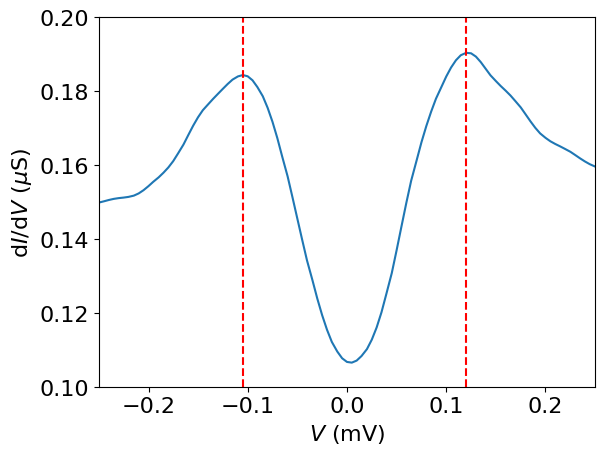
\includegraphics[width=\textwidth]{Discussion/AuNbV3DF_VcExtraction.png}
         \caption{Differential conductance of AuNb device with 50 nm niobium, measured at 30 mK, with the extracted $V_C$ values shown as red dashed lines.}
         \label{subfig:}
     \end{subfigure}
     \caption{dI/dV calculated from IV measurements, and their extracted $V_C$ values.}
     \label{fig:Vc_Extraction}
        
\end{figure}

We did this extraction for all devices for which the differential conductance shows superconducting coherence peaks. Two out of the four AuNb devices with 50 nm niobium show coherence peaks, and all four of the AuNb devices with 60 nm bridge spacing show coherence peaks. Both the AuNb devices with 50 nm niobium show critical voltages of 0.11 mV, and in the plots of the AuNb devices with 60 nm bridge spacing show critical voltages of 0.56 mV $\pm$0.16 mV . As the coherence peaks in S-I-S junctions appear at $V_C = \pm 2\Delta/e$, this allows us to estimate the average size of the induced energy gap at the tip of the leads, $\Delta_\mathrm{prox}$, to be 55 $\mu$eV and 280 $\mu$eV respectively. 

The fact that no superconducting features were observed in the IV measurements of the PdNb and AuNb indicates that either there was no induced superconducting energy gap at the tips of the leads, or that the gap was too small to be resolved. 

Only two of the four AuNb devices with 50 nm niobium showed superconductance features while all four of the four AuNb devices with 60 nm bridge spacing. This might be due to fact that the location of the tunneling gap induced through electromigration is less consistently in the center of the bridge in the AuNb devices with 50 nm niobium than in the devices with 60 nm bridge spacing. The belief that the location of the tunneling gap is less consistently at the center of the bridge for the 50 nm niobium is motivated by the fact that the center of the bridge in those devices has a double layer of gold, making the local current density and the local resistance smaller and therefore the likelihood of an electromigration induced break lower in this region, as discussed in section 5.1. In those devices where the tunnel gap forms very close to one end of the bridge, migration happens in a region where Ti and Nb are likely to be present. As discussed in the section on electromigration results, many of the devices, after they had been migrated, showed an increase in resistance when they were cooled down. This resistance increase was reversed as they were warmed back to room temperature. This type of behavior is associated with semiconductors. A possible interpretation would therefore be that when electromigration takes place far away from the center, other kinds of material such as titanium oxide for example, are mixed into the bridge material at the tunnel interface, leading to semi-conductor like behavior there. Since such a mixture has many more scattering sites than a pure metal, the diffusion would be poor which could explain the lack of observed superconductivity.  

If we compare the induced energy gaps in the devices after electromigration to the Thouless energies before electromigration, we see that the induced energy gap of the AuNb junctions with 50 nm niobium are of the same order as the determined Thouless energy of the unbroken junctions, while the induced gap in the AuNb junctions with 60 nm spacing is approximately 8 times as large as its Thouless energy before breaking. Since $L$ is halved after breaking if the break happens in the middle of the junction, and the Thouless energy scales as $1/L^2$, we expect a four-fold increase if all else stays the same. Since we see no change in the AuNb devices with 50 nm niobium thickness, and an eight-fold increase in the AuNb devices with 60 nm spacing, we can conclude that the structure of the device changes is changed during the electromigration process. The reason that the AuNb device with 50 nm niobium does not experience the four-fold increase in gap size expected based on the geometric argument may be due to the fact that the electromigration causes Ti or Nb atoms to be mixed into the Pd, which increases scattering and reduces the Thouless energy. The reason that the AuNb devices with 60 nm bridge spacing achieve an eight-fold increase might be due to the rearranging of grain boundaries, which could improve the diffusion in the gold and thereby increase the effective energy gap at the tip of the leads. In order for this effect to cause a two-fold increase in the gap, however, the mean free path would have to increase four-fold, which seems unreasonable.   

\subsection*{Andreev Reflections}

The differential conductances of three of the devices with 60 nm bridge spacing show shoulders inside the gap. 


\begin{figure}[H]
     %These plots come from numid 2 from PdNb chip 6
     \centering
     \begin{subfigure}[t]{0.49\textwidth}
         \centering
         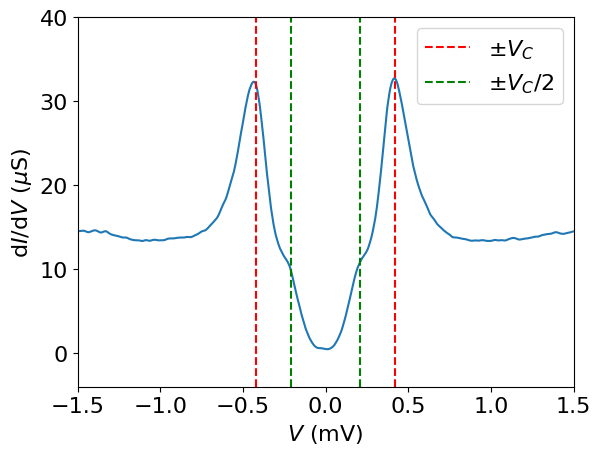
\includegraphics[width=\textwidth]{Discussion/Shoulders_106.png}
         \caption{Differential conductance of AuNb device with 60 nm bridge spacing, measured at 25 mK, with the extracted $V_C$ values shown as red dashed lines.}
         \label{subfig:}
     \end{subfigure}
     \hfill
     \begin{subfigure}[t]{0.49\textwidth}
         \centering
         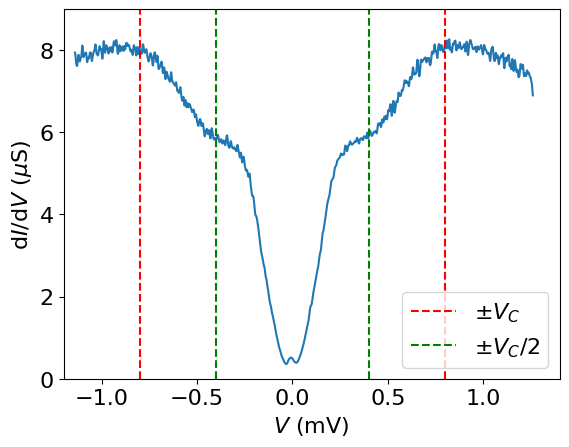
\includegraphics[width=\textwidth]{Discussion/Shoulders_70.png}
         \caption{Differential conductance of AuNb device with 50 nm niobium, measured at 30 mK, with the extracted $V_C$ values shown as red dashed lines.}
         \label{subfig:}
     \end{subfigure}
     \caption{dI/dV calculated from IV measurements, and their extracted $V_C$ values as well as the locations of the shoulders.}
     \label{fig:Shoulders_at_vc_over2}
        
\end{figure}

We attribute these shoulders to multiple Andreev reflections. When the induced energy gaps are equal on both sides of the tunnel gap, multiple Andreev reflections cause peaks in the differential conductance at $V = 2\Delta / ne$, where $n = 1,2,3,\ldots$. The size of the $n^\mathrm{th}$ peak drops off exponentially with $n$, with a decay rate dependent on the interface transparency and the phase coherence length. In the plots in figure \ref{fig:Shoulders_at_vc_over2} we can identify only the first order contribution. When the energy gaps at the tips of the leads of the SEMBJ are not equal, the locations of the Andreev reflection peaks follow a more complicated pattern, where the locations of the peaks are proportional to the energy gap at either end of the tunnel gap, or to the sum of these energy gaps. 

That the locations of the shoulders correspond to $V_C/2$ is evidence that the energy gaps are approximately equal on both sides of the tunnel gap. Since the induced energy gap is a function of the distance to the superconductor, this is evidence that the gap is forming close to the center.  

\subsection{Asymmetric Critical Current}

The results in section 4.6 show that all our devices show an asymmetric critical current upon applying a magnetic field in the perpendicular in-plane direction. This asymmetry persists across all stages of electromigrated breaking, from before any breaking has taken place until the tunnel regime. The AuNb devices with 60 nm spacing also show an asymmetry in the critical current when the magnetic field is applied in the out of plane direction. This may be attributable to the fact that the niobium layer is off-centered in those devices. That the niobium layer is off-centered means that it also somewhat resembles as an SN layer in the direction perpendicular to the current, but to a much smaller degree than in the out of plane direction. This might explain why we see this out of plane asymmetry in only those devices. 

The fact that the asymmetry of the junctions persists as the diameter of the bridge shrinks is significant, since it implies that an explanation of the asymmetry in terms of a self-field effect is less likely; since the current in those devices is very small, the strength of the generated field is correspondingly small. The characteristic magnetic field scale also remains approximately constant during the breaking process.

The consistency with which the asymmetric critical current as a function a perpendicular in-plane magnetic field is exhibited by our devices is significant since it implies that this device design can be used as a simple lithographic platform for fabricating asymmetric critical current based devices.

\subsection{Suggested Design improvements}

Based on the discussion so far, we can suggest further design changes that are likely to improve the quality of the SEMBJs. 

Since the niobium proximitizes the gold in the AuNb bilayer so strongly that the bilayer energy gap is equal to the energy gap of the bare niobium layer to within the order of one percent, we expect that the benefit increasing the thickness of the gold layer further has on the diffusion constant in the bridge will outweigh the negative effect this change has on the bilayer energy gap. Increasing the thickness of the gold would also reduce the resistivity of the bridge and make electromigration more difficult to control. However, since the results show that electromigration is highly controllable in the AuNb devices with 60 nm spacing, the level of control would remain sufficiently high even if it was reduced somewhat.

The overlap of the two gold layers in the center of the bridge in the AuNb devices with 50 nm niobium was dealt with by increasing the spacing between the two sides of the bowtie in the design. Although this removed the region of overlap, a negative side effect of this solution is that the distance from the center of the bridge to the superconductor is increased, which reduces the induced gap at the center of the bridge. An alternative solution that would not have this drawback, is to reduce the angle at which the gold layers are evaporated while keeping the bridge length the same. A potential drawback of this solution is that, since the niobium layer is placed closer to the center of the bridge, some niobium particles may be more likely to end up at the center of the bridge which might cause the contacts of the SEMBJ to be contaminated. Investigating the viability of this approach would be worthwhile.

It was mentioned in the introduction to this thesis that creating palladium based SEMBJs was of interest. As mentioned in the methods and results, it was thought that the optimizations made to the gold based SEMBJ design would also lead to improvements in the palladium based design, if palladium was resubstituted for gold. Due to time constraints, testing this hypothesis was outside the scope of this thesis, but doing so would have been an obvious next step if time had allowed for it.











\section{Conclusion and Outlook}
\label{section:Conclusion}





The goal was to find a device design and fabrication method that would result in optimal superconductance at the tips of the leads of the SEMBJ. The most important parameter determining the quality of the superconductance is the size of the induced energy gap at the tips of the leads. The reason that this parameter is important is that it determines the voltage bias range in which the device operates in the superconducting regime; for bias voltages outside the range determined by this energy gap, transport happens normally and the reasons for using an SEMBJ over a regular EMBJ are lost. 

The space of device designs and fabrication methods was constrained to only include bowtie geometry constrictions fabricated using shadow mask double angle evaporation. The only superconductor that was evaluated was niobium. The parameters that were varied during the optimization of the design were the thicknesses of the bridge layer and the superconducting layer, and the length of the bridge. The devices were electromigrated using feedback controlled electromigration, both at room temperature and at low temperature. The devices were characterized both before and after electromigration using low temperature transport measurements and SEM imaging. The results of these characterizations were used to inform the subsequent designs during each design iteration. 

This chapter summarizes the main findings of this thesis, evaluates their significance, discusses their limitations and suggests possible avenues for future research. 


\subsection{Summary of Main Findings}

There are several important conclusions that can be drawn from the results in this thesis. The main conclusions are listed here. 

\begin{itemize}

\item It is possible to create proximity induced superconducting electromigrated breakjunctions using double angle shadow mask evaporation and feedback controlled electromigration in a bowtie geometry.

\item It is possible to proximitize palladium and gold films using this method.

\item Our experiments resulted in a proximity-induced energy gap of approximately 0.28 meV at the tips of the leads of the SEMBJ. This gap size is comparable to values reported in previous studies, indicating that our device design and fabrication method are effective for achieving high-quality superconductivity in this type of junction. The ability to simply and reliably produce proximity-induced gaps of this magnitude is an important step toward realizing practical applications of these devices and for future research.

\item Good control over the location of the electromigration-induced break in the device is necessary to ensure a large energy gap at the ends of both leads.

\item The results of this study demonstrate that bowtie constricted gold films with a thickness of 15 nm can be successfully electromigrated with a high degree of control. These findings suggest that it may be feasible to increase the thickness of the gold films while maintaining sufficient control over the electromigration process.

\item The results of this study suggest that a 50 nm thick niobium layer is capable of inducing superconductivity in a 30 nm thick gold layer, resulting in an energy gap within one percent of that of pure niobium. These findings imply that it may be possible to further increase the thickness of the gold while maintaining a sufficient bilayer energy gap.

\item The devices show an asymmetric critical current upon applying a magnetic field in the perpendicular in-plane direction. Our device design offers a simple lithographic platform for making Josephson-diode based devices.

\end{itemize}





\subsection{Suggested Future Research}

As mentioned, the resubstitution of palladium for the bridge material in the device design was not researched due to time constraints. Testing devices of this type would be an obvious next step in continuing this research.

Strong correlations were found between the $I_CR_N$ products of the devices and their normal state resistances. Having knowledge and control of such correlations could be a valuable prognostic tool, that could be used to pre-select especially promising devices based on simple room temperature measurements. Exploring this correlation further would therefore be of great interest.

The fabrication and measurements of the kinds of devices studied in this thesis is a slow process, which necessarily limits the number of design parameters that can be studied. Continued exploration of the possible device designs is necessary for further progress. An interesting design variation that could be explored in future work is an SEMBJ where the normal metal is sandwiched in between two superconducting layers in an SNS sandwich, instead of only being proximitized from one side in an SN bilayer design as was studied in this thesis. This design could be realized using the same shadow mask that was used during this thesis with no changes or only minimal changes, and seems intuitively better suited for inducing superconductivity than an SN bilayer design.

In this thesis we showed that our devices possess an asymmetric critical current upon applying a magnetic field in the perpendicular in-plane direction. Future research can build on this finding by exploring variations on the design. 

\subsection{Concluding Remarks}

The goal of this thesis, to create an SEMBJ, was reached. The fabrication method that was used throughout this thesis stands out due to its simplicity and swiftness; it contains only a single e-beam step, and many dozens of devices can be made in only a few hours. This is a significant advantage that allows for rapid device design changes and cheaper and faster experiments. Even when the design is changed to incorporate a local back gate, it remains simple compared to many alternative fabrication methods. The induced gap at the leads of the SEMBJ, which reached 280 $\mu$eV in our final design, is of the same order or larger than many devices found in the literature, indicating that our method is effective for achieving high-quality superconductivity in this type of junction. Additionally, the devices were found to have a magnetic field dependent directional asymmetry in their critical current at each stage of breaking. This phenomenon is currently not well understood, and the findings in this thesis may help guide future research.



\addcontentsline{toc}{section}{Bibliography}
\section*{Bibliography}


 
[1] Sawtelle, S.D., 2018. Electromigration and Electrothermal Properties in Gold Nanostructures (Doctoral dissertation, Yale University).

[2] Moore, G.E., 1998. Cramming more components onto integrated circuits. Proceedings of the IEEE, 86(1), pp.82-85.


[3] Tang, C.L., 2005. Fundamentals of quantum mechanics: for solid state electronics and optics. Cambridge University Press.

[4] Nazarov, Y.V. and Blanter, Y.M., 2009. Quantum transport: introduction to nanoscience. Cambridge University Press.

[5] Combescot, R., 2022. Superconductivity: An Introduction. Cambridge University Press.

[6] Golubov, A.A., Wilhelm, F.K. and Zaikin, A.D., 1997. Coherent charge transport in metallic proximity structures. Physical Review B, 55(2), p.1123.

[7] de Bruijckere, J., 2020. Correlated Spin Phenomena in Molecular Quantum Transport Devices (Doctoral dissertation, Delft University of Technology).

[8] Gehring, P., Thijssen, J.M. and van der Zant, H.S., 2019. Single-molecule quantum-transport phenomena in break junctions. Nature Reviews Physics, 1(6), pp.381-396.

[9] Wang, X., Ouyang, Y., Jiao, L., Wang, H., Xie, L., Wu, J., Guo, J. and Dai, H., 2011. Graphene nanoribbons with smooth edges behave as quantum wires. Nature Nanotechnology, 6(9), pp.563-567.

[10] Jiao, L., Wang, X., Diankov, G., Wang, H. and Dai, H., 2010. Facile synthesis of high-quality graphene nanoribbons. Nature Nanotechnology, 5(5), pp.321-325.

[11] Ho, P.S. and Kwok, T., 1989. Electromigration in metals. Reports on Progress in Physics, 52(3), p.301.

[12] Baumans, X., 2018. Nano-engineering superconducting junctions by atomic migration.

[13] Likharev, K.K., 1979. Superconducting weak links. Reviews of Modern Physics, 51(1), p.101.

[14] Heida, J. P. (1998). Josephson currents in two dimensional mesoscopic ballistic conductors. [Thesis fully
internal (DIV), University of Groningen]. s.n.

[15] Martinis, J.M., Hilton, G.C., Irwin, K.D. and Wollman, D.A., 2000. Calculation of Tc in a normal-superconductor bilayer using the microscopic-based Usadel theory. Nuclear Instruments and Methods in Physics Research Section A: Accelerators, Spectrometers, Detectors and Associated Equipment, 444(1-2), pp.23-27.

\newpage
%\setlength{\textwidth}{22cm}
\newgeometry{left=1cm, right = 1cm, top = 1cm, bottom = 2cm}

\section{Appendix}

\subsection{A: SEM Images Fabrication Results}
\subsubsection*{A1: PdNb}

\begin{figure}[h]
     \centering
     \begin{subfigure}[b]{\textwidth}
         \centering
         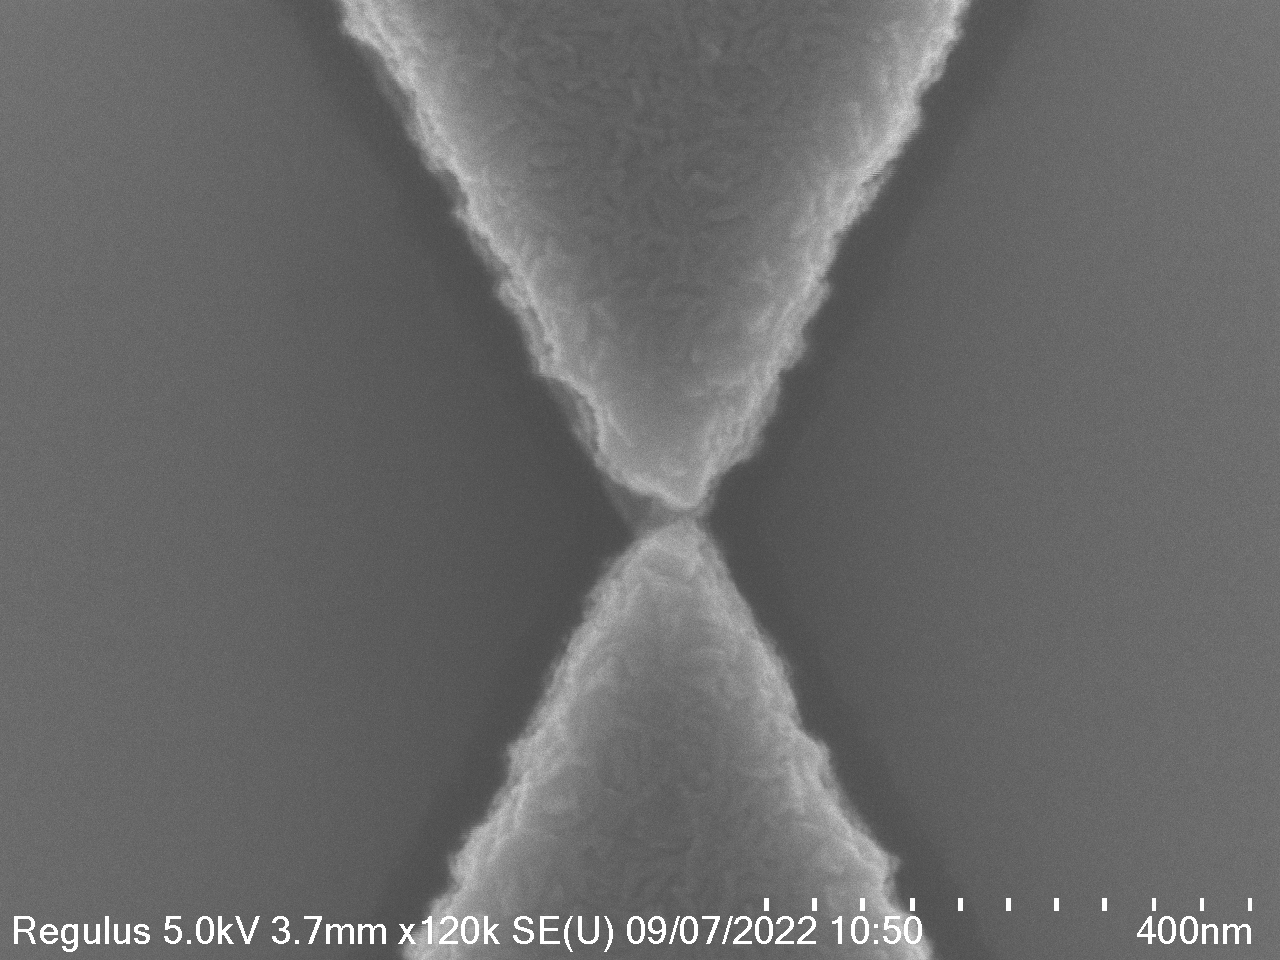
\includegraphics[width=0.32\textwidth]{TiPdPdNbSEMBJ1_31_1300uCcm2_0003_1.png}
         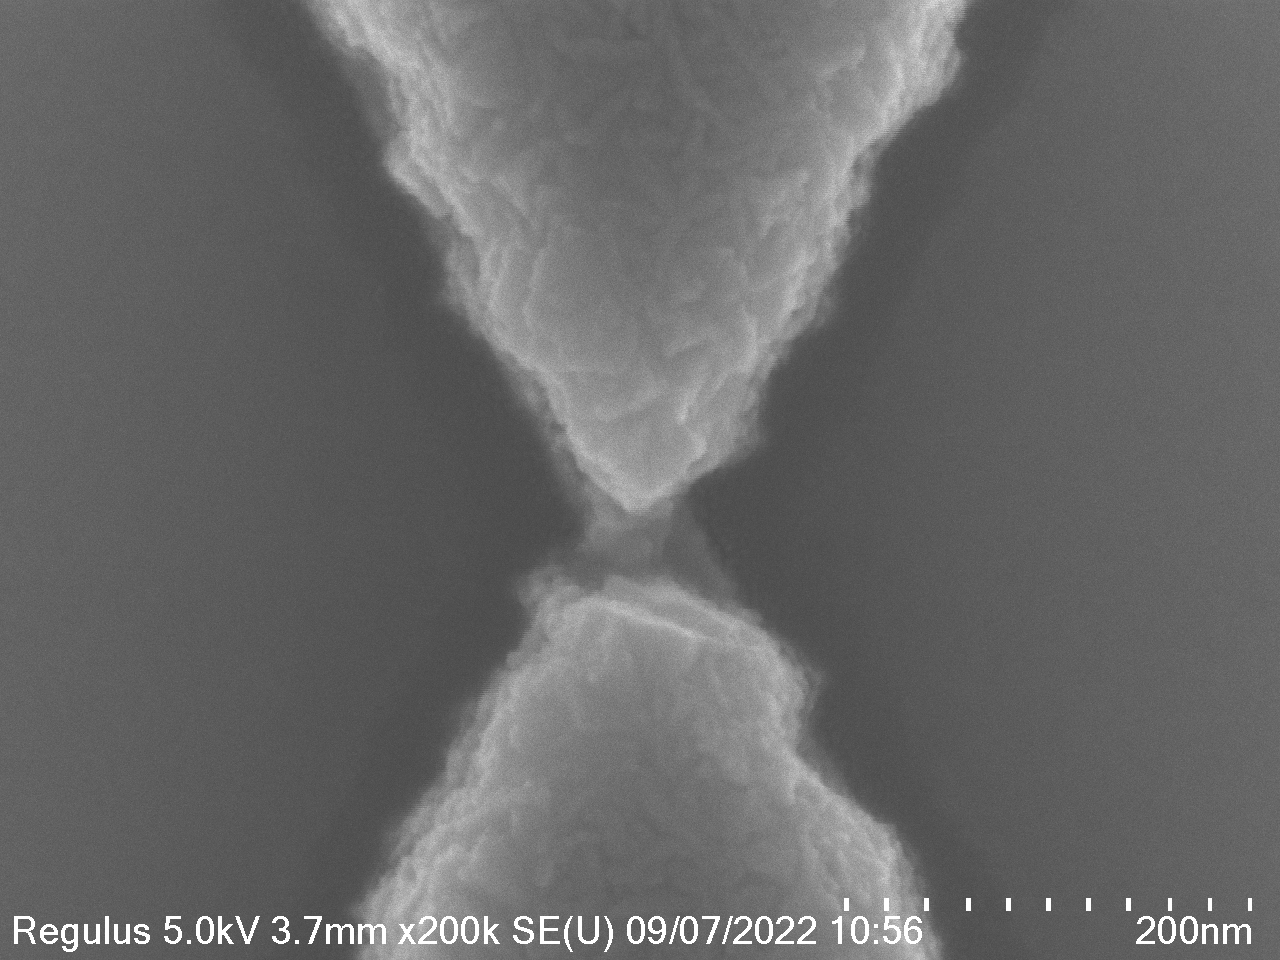
\includegraphics[width=0.32\textwidth]{TiPdPdNbSEMBJ1_31_1320uCcm2_0001_1.png}
         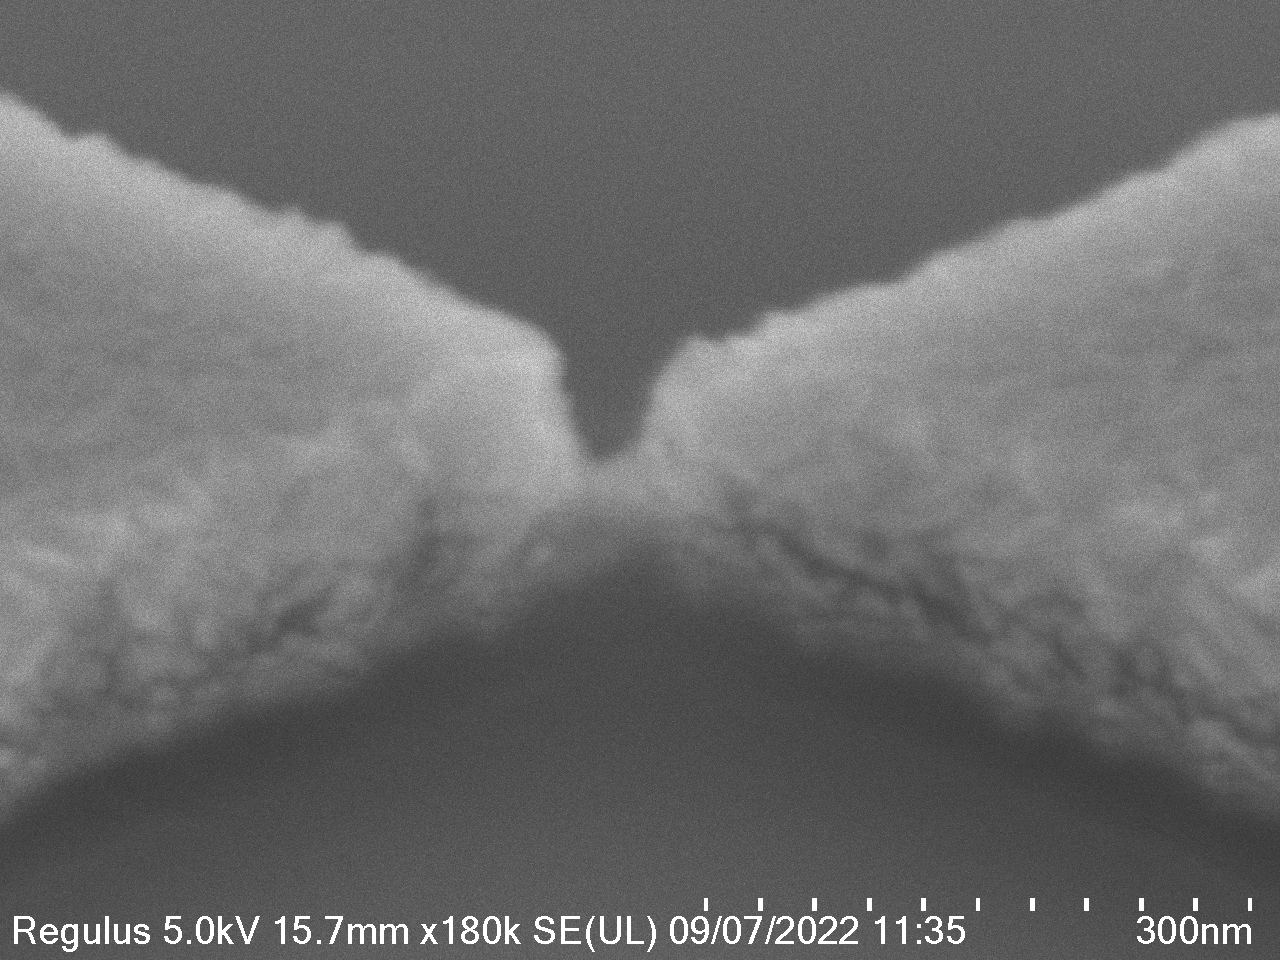
\includegraphics[width=0.32\textwidth]{TiPdPdNbSEMBJ1_31_1320uCcm2_0013_1.png}
         %\caption{A portion of the resist is irradiated with an electron beam in as specified pattern.}
         %\label{c}
     \end{subfigure}
     %\hfill
     \begin{subfigure}[b]{\textwidth}
         \centering
         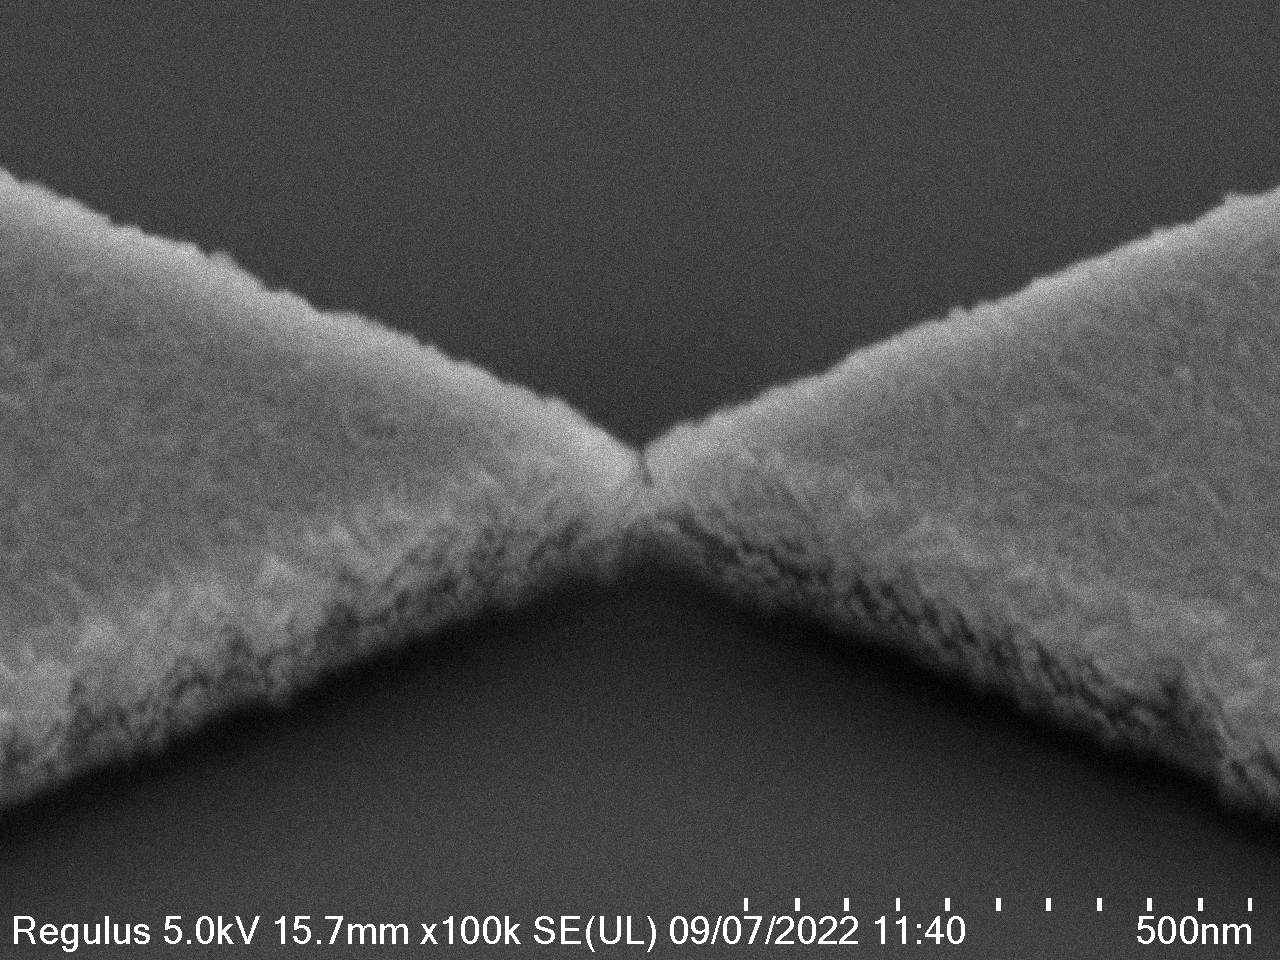
\includegraphics[width=0.32\textwidth]{TiPdPdNbSEMBJ1_31_1340uCcm2_0002_1.png}
         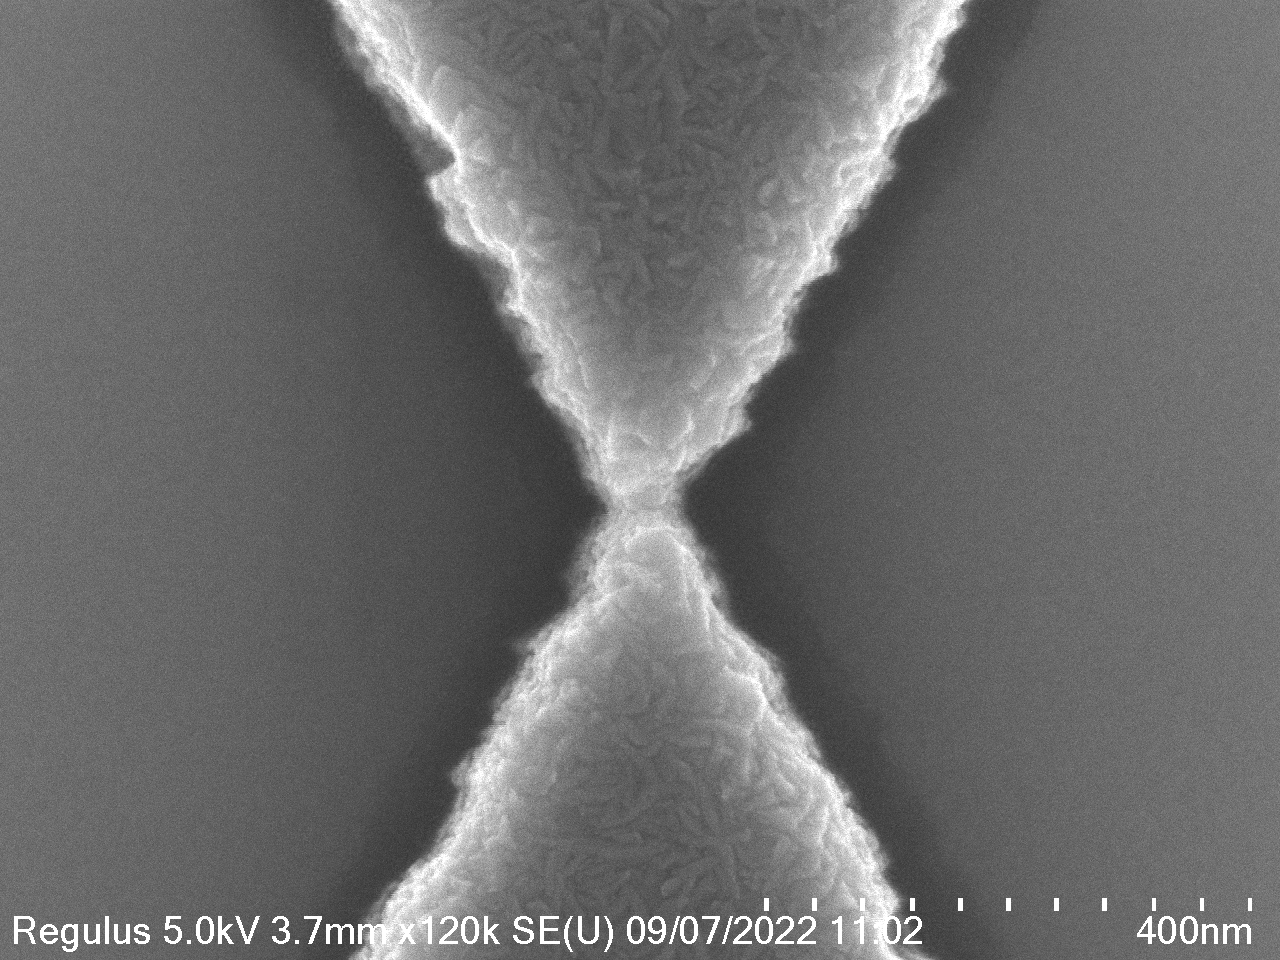
\includegraphics[width=0.32\textwidth]{TiPdPdNbSEMBJ1_31_1660uCcm2_0002_1.png}
         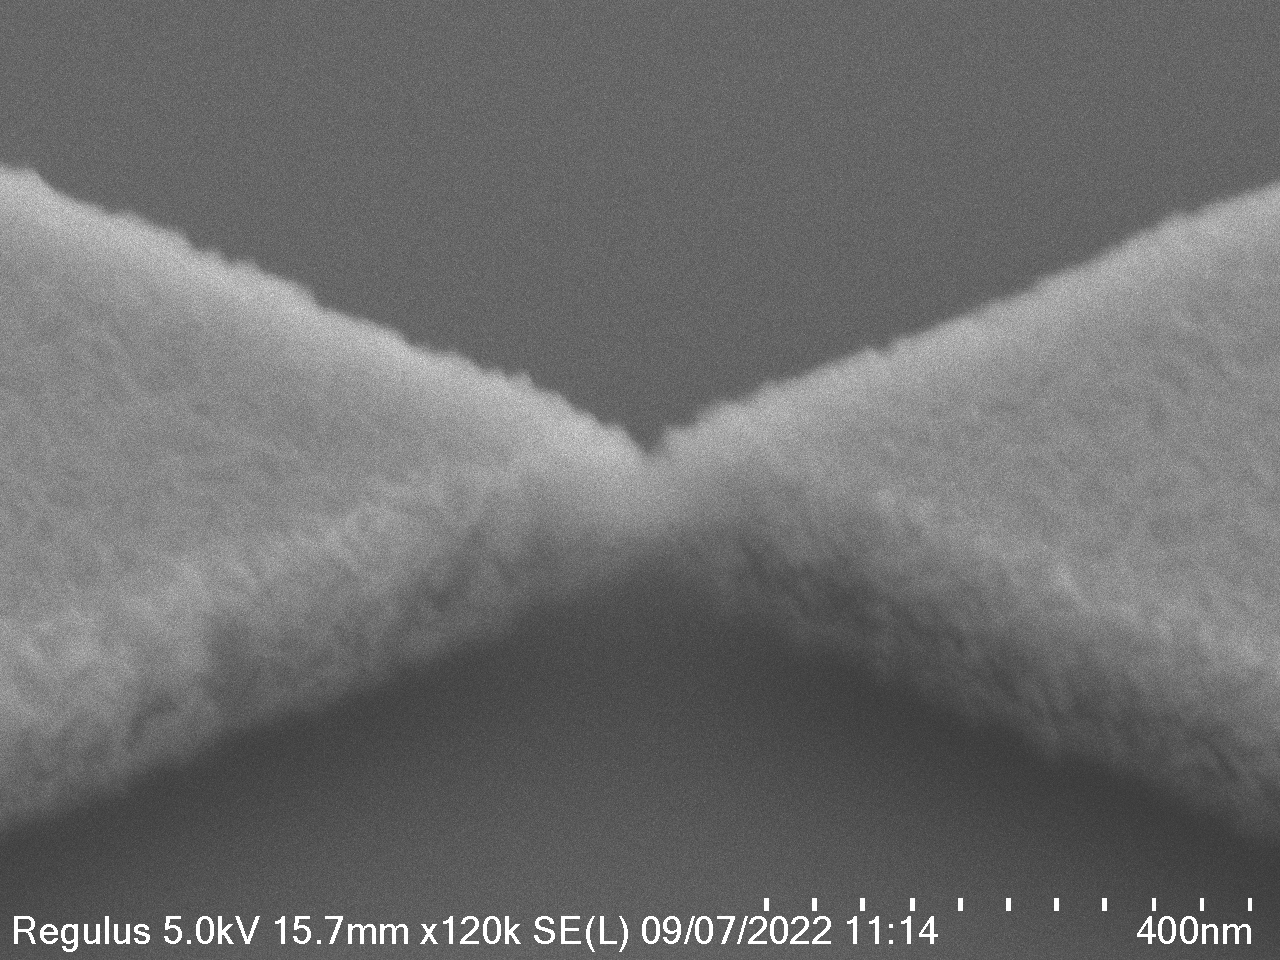
\includegraphics[width=0.32\textwidth]{TiPdPdNbSEMBJ1_31_1660uCcm2_0006_1.png}
         %\caption{A portion of the resist is irradiated with an electron beam in as specified pattern.}
         %\label{c}
     \end{subfigure}
        \caption{SEM images of PdNb devices.}
        \label{fig:}
        
\end{figure}
\vspace{-1cm}

\subsubsection*{A2: AuNb, 100 nm Nb}

\begin{figure}[H]
     \centering
     \begin{subfigure}[b]{\textwidth}
         \centering
         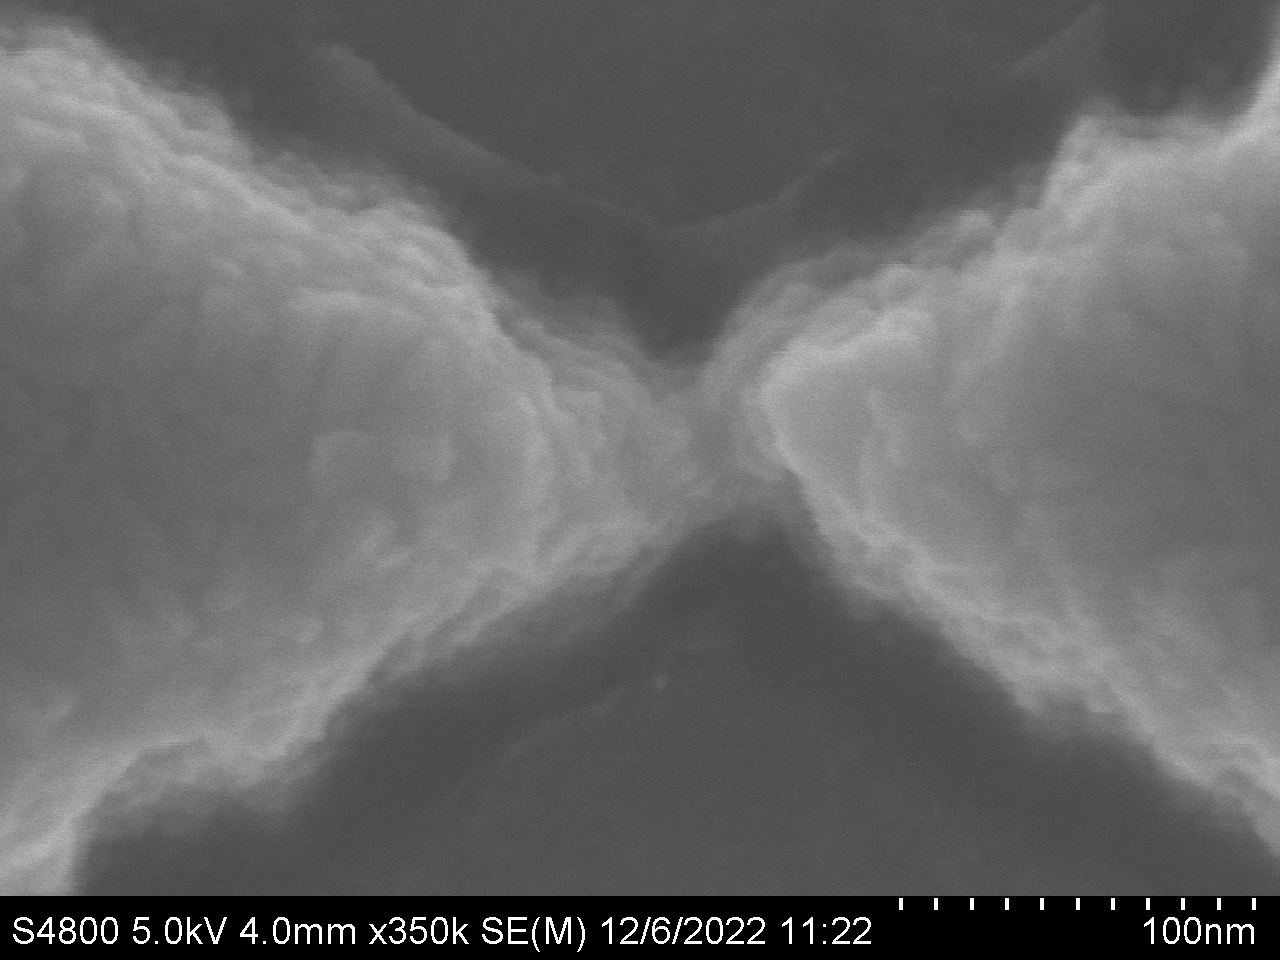
\includegraphics[width=0.32\textwidth]{Appendix_A/A2.png}
         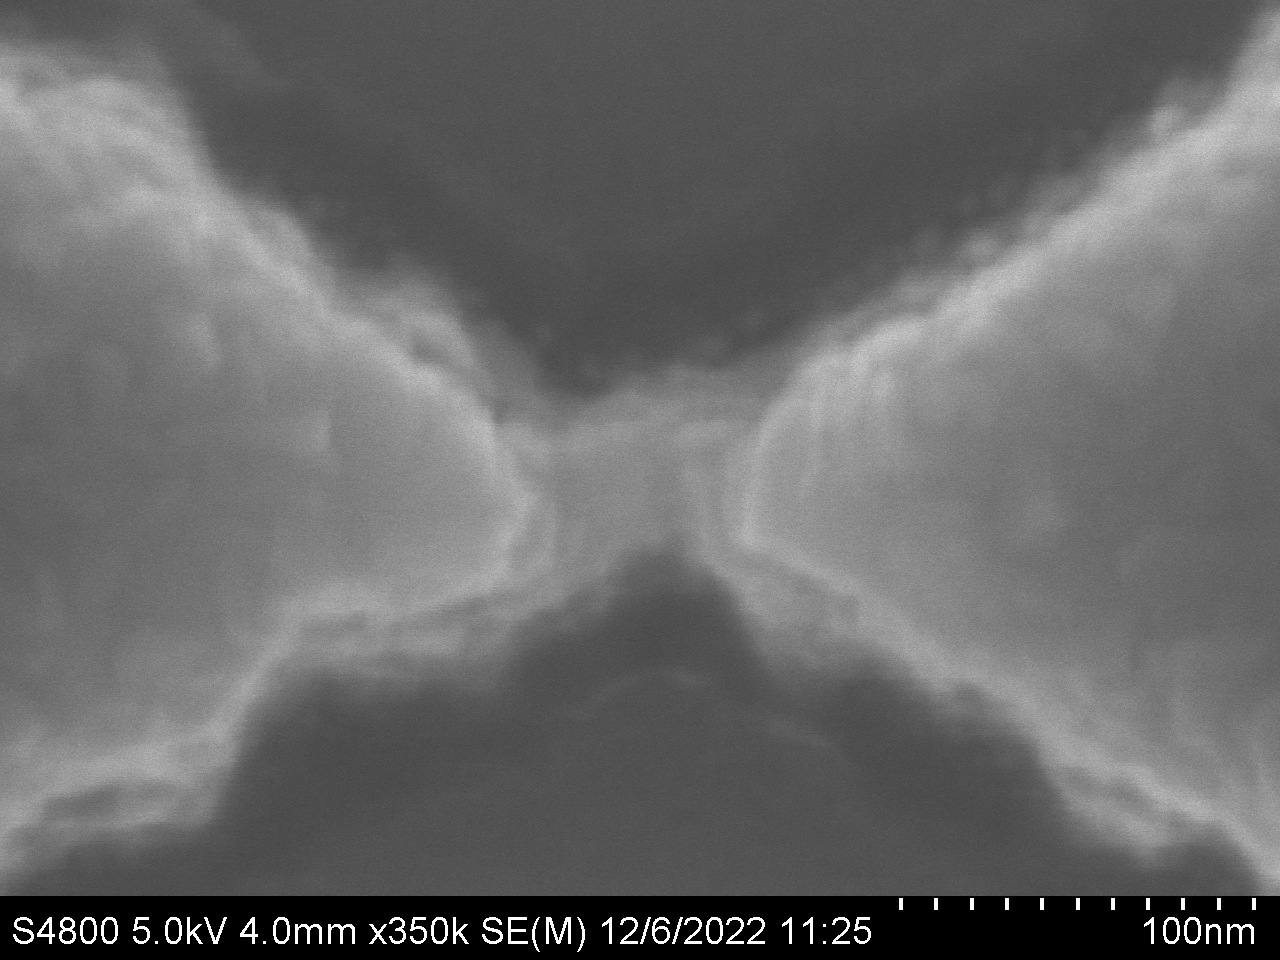
\includegraphics[width=0.32\textwidth]{Appendix_A/A5.png}
         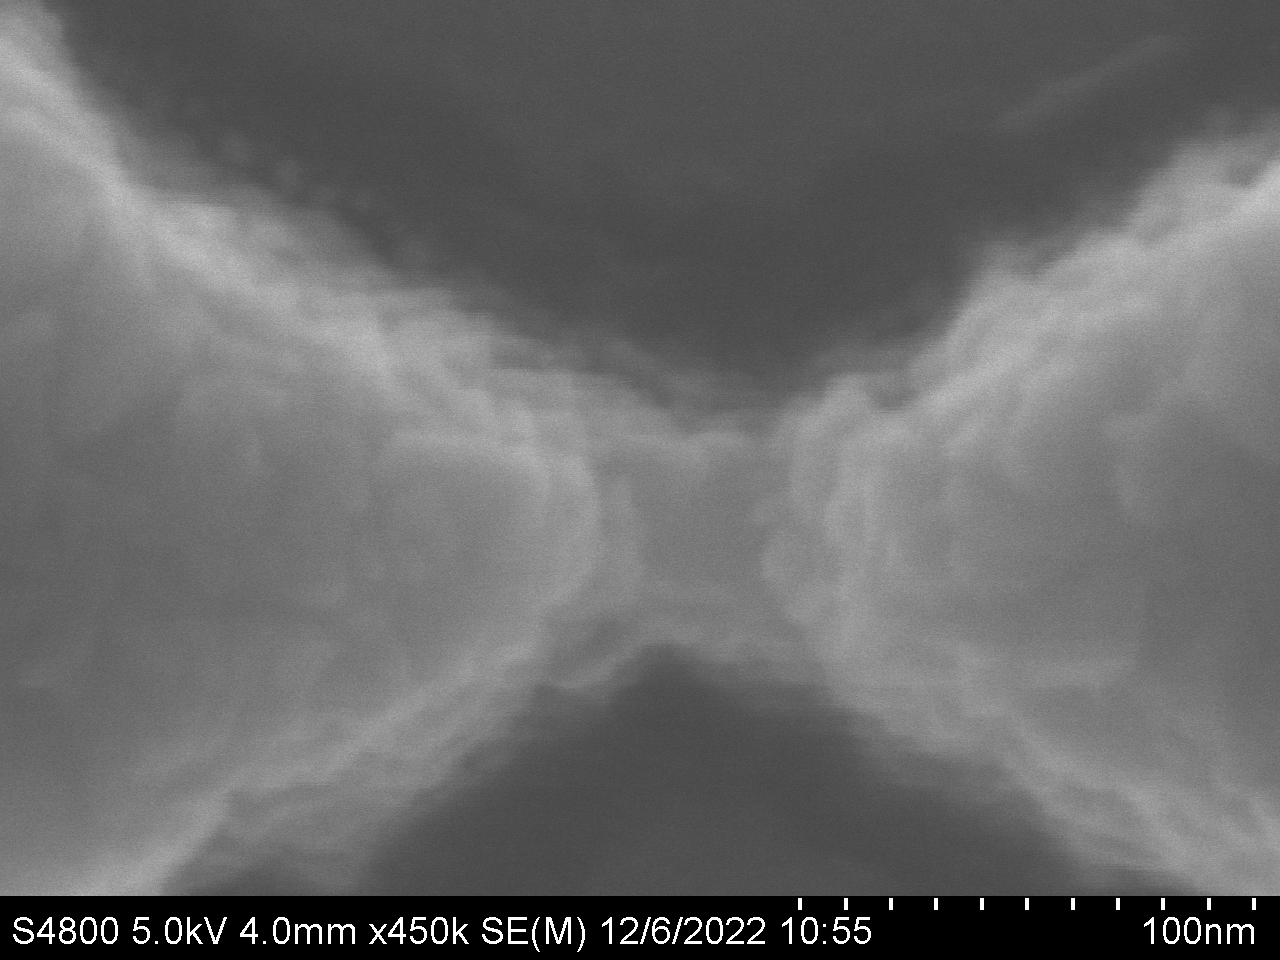
\includegraphics[width=0.32\textwidth]{Appendix_A/E4.png}
         %\caption{A portion of the resist is irradiated with an electron beam in as specified pattern.}
         %\label{c}
     \end{subfigure}
     %\hfill
     \begin{subfigure}[b]{\textwidth}
         \centering
         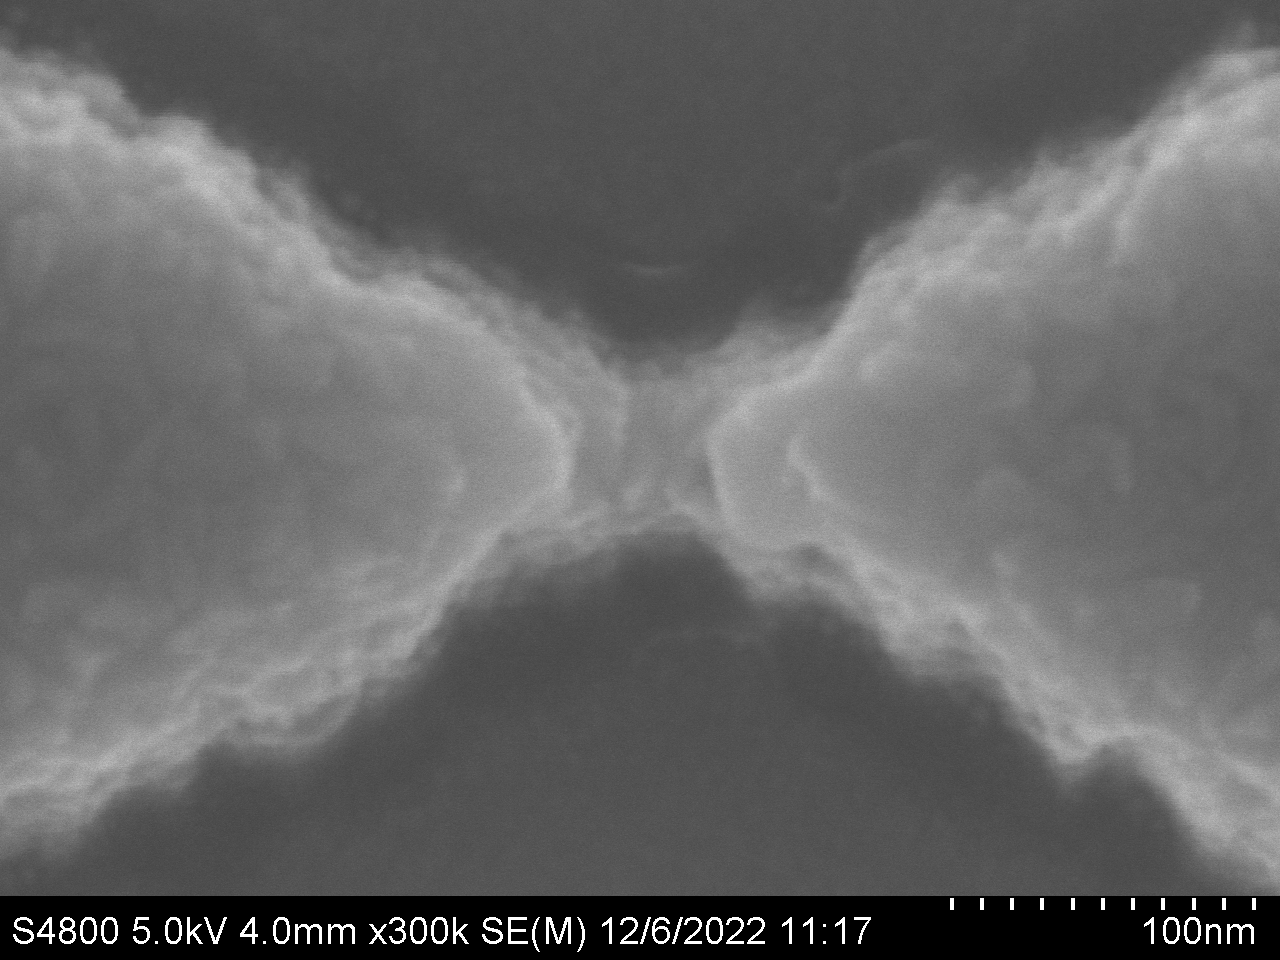
\includegraphics[width=0.32\textwidth]{Appendix_A/C1.png}
         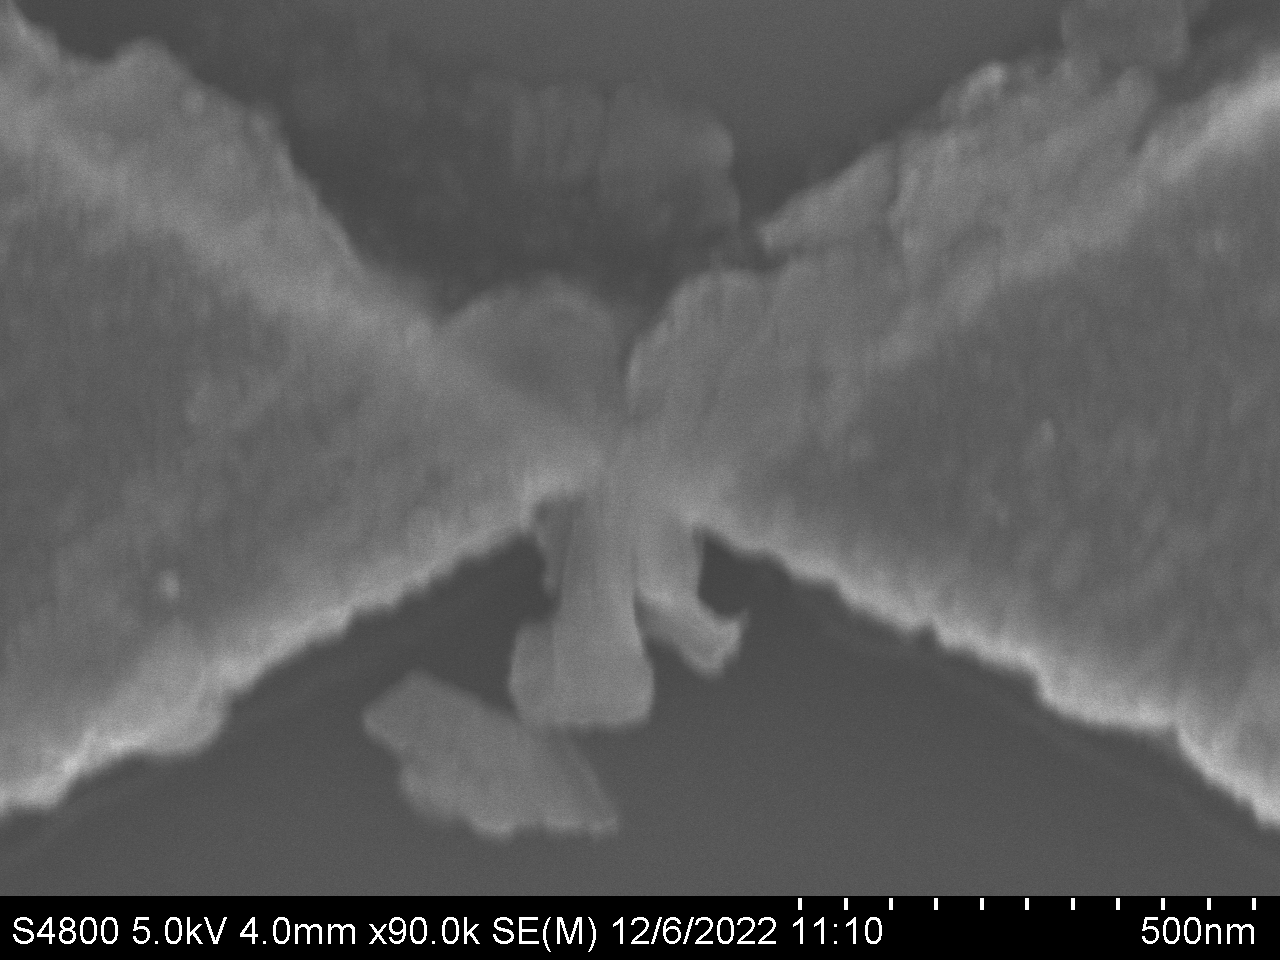
\includegraphics[width=0.32\textwidth]{Appendix_A/D8_2.png}
         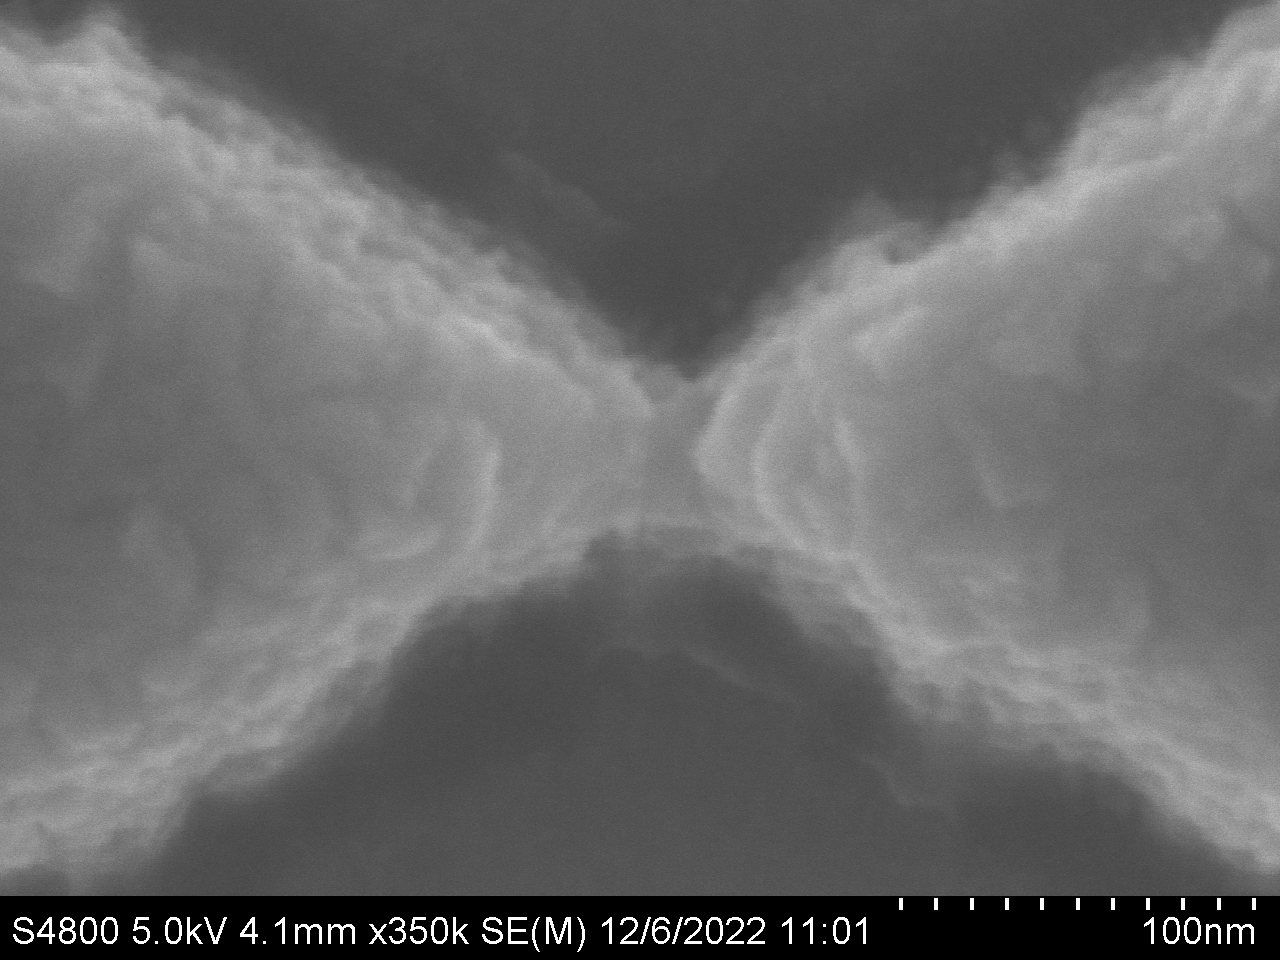
\includegraphics[width=0.32\textwidth]{Appendix_A/E6.png}
         %\caption{A portion of the resist is irradiated with an electron beam in as specified pattern.}
         %\label{c}
     \end{subfigure}
        \caption{SEM images of AuNb devices with a 100 nm niobium layer.}
        \label{fig:}
        
\end{figure}

\subsubsection*{A3: AuNb, 50 nm Nb}
\begin{figure}[H]
     \centering
     \begin{subfigure}[b]{\textwidth}
         \centering
         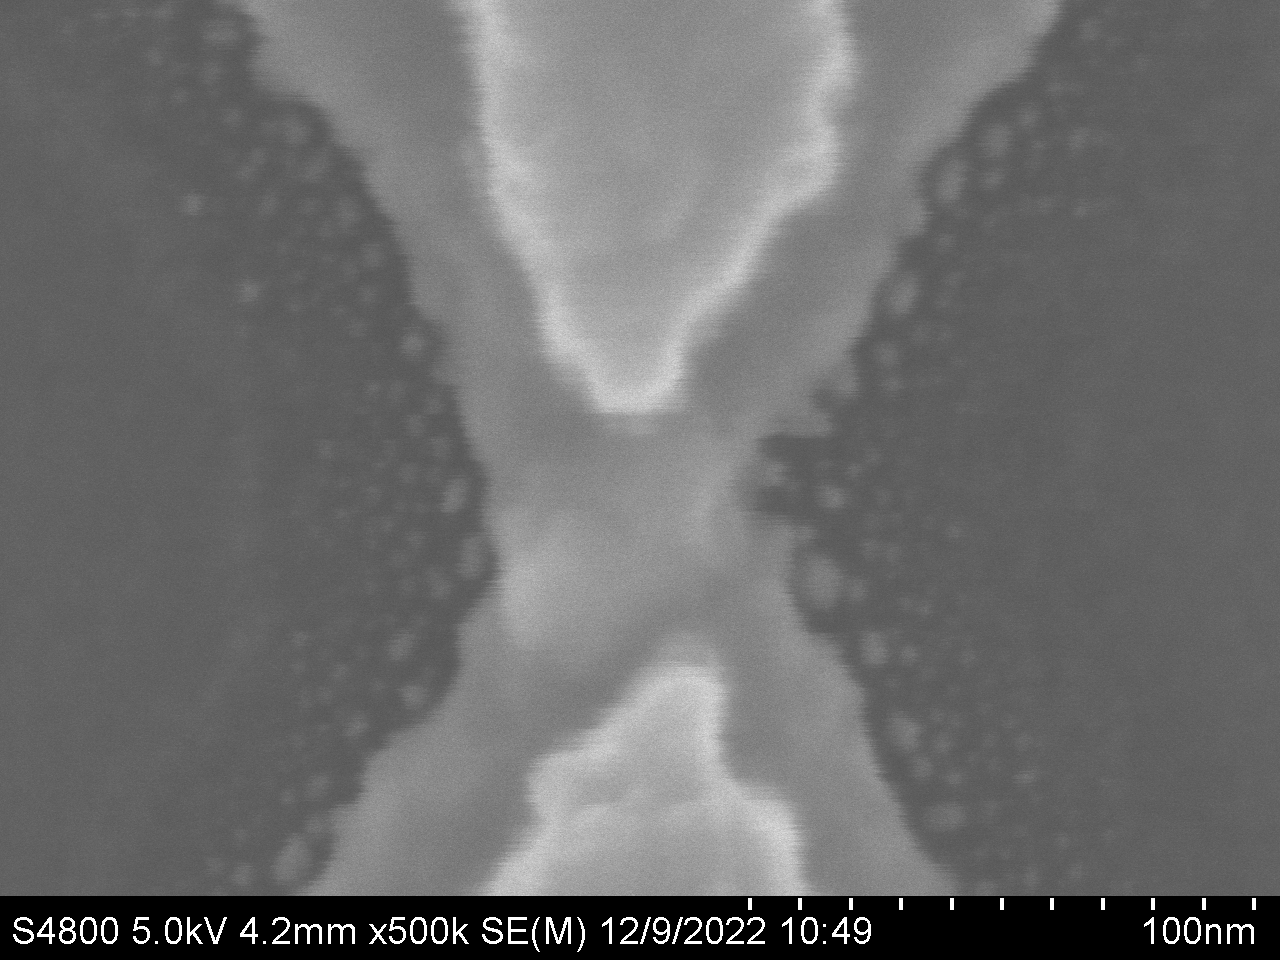
\includegraphics[width=0.32\textwidth]{Appendix_A/A3/A1.png}
         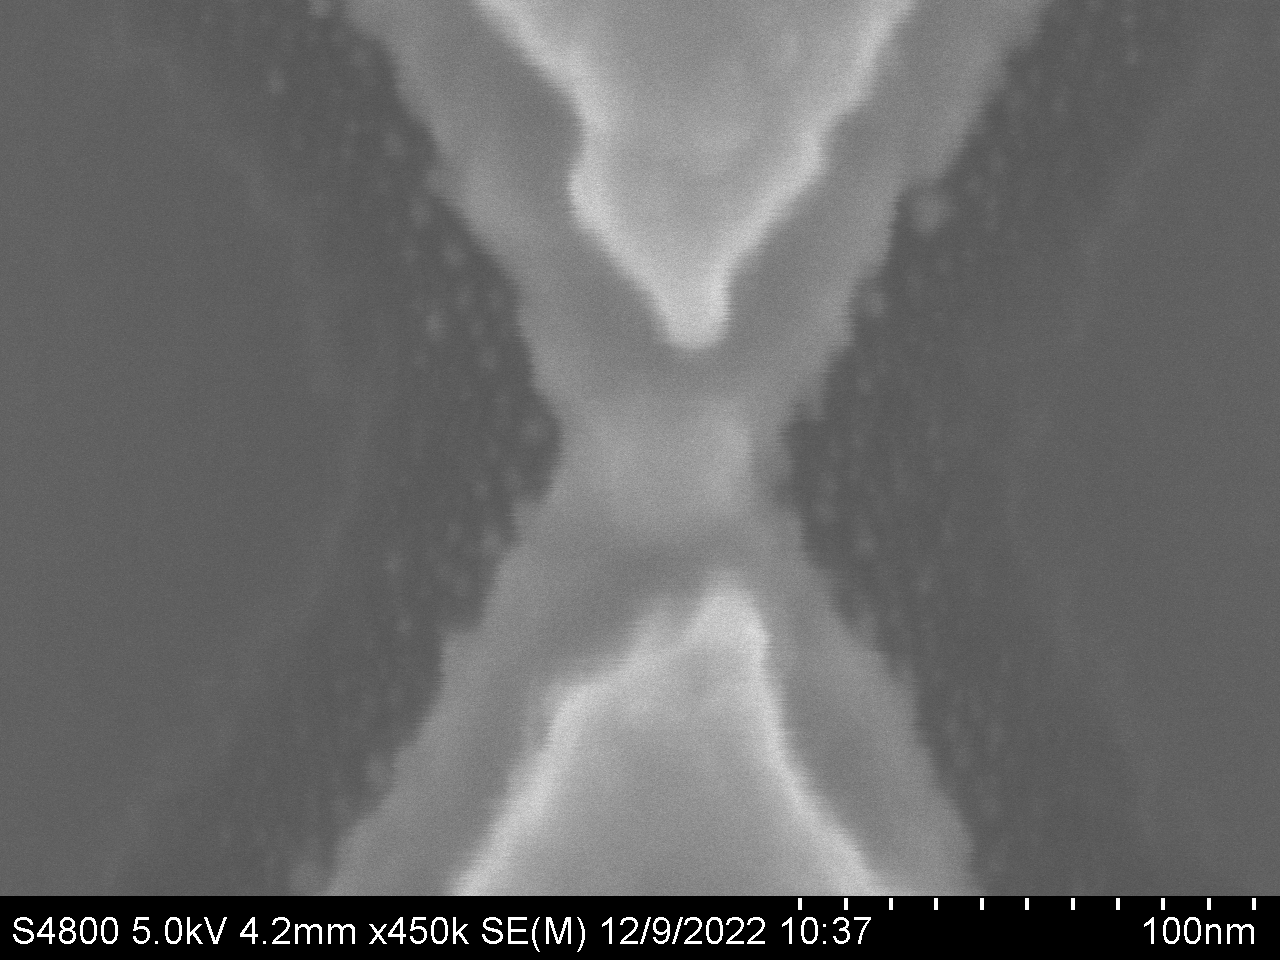
\includegraphics[width=0.32\textwidth]{Appendix_A/A3/A1_Alternate_contrast.png}
         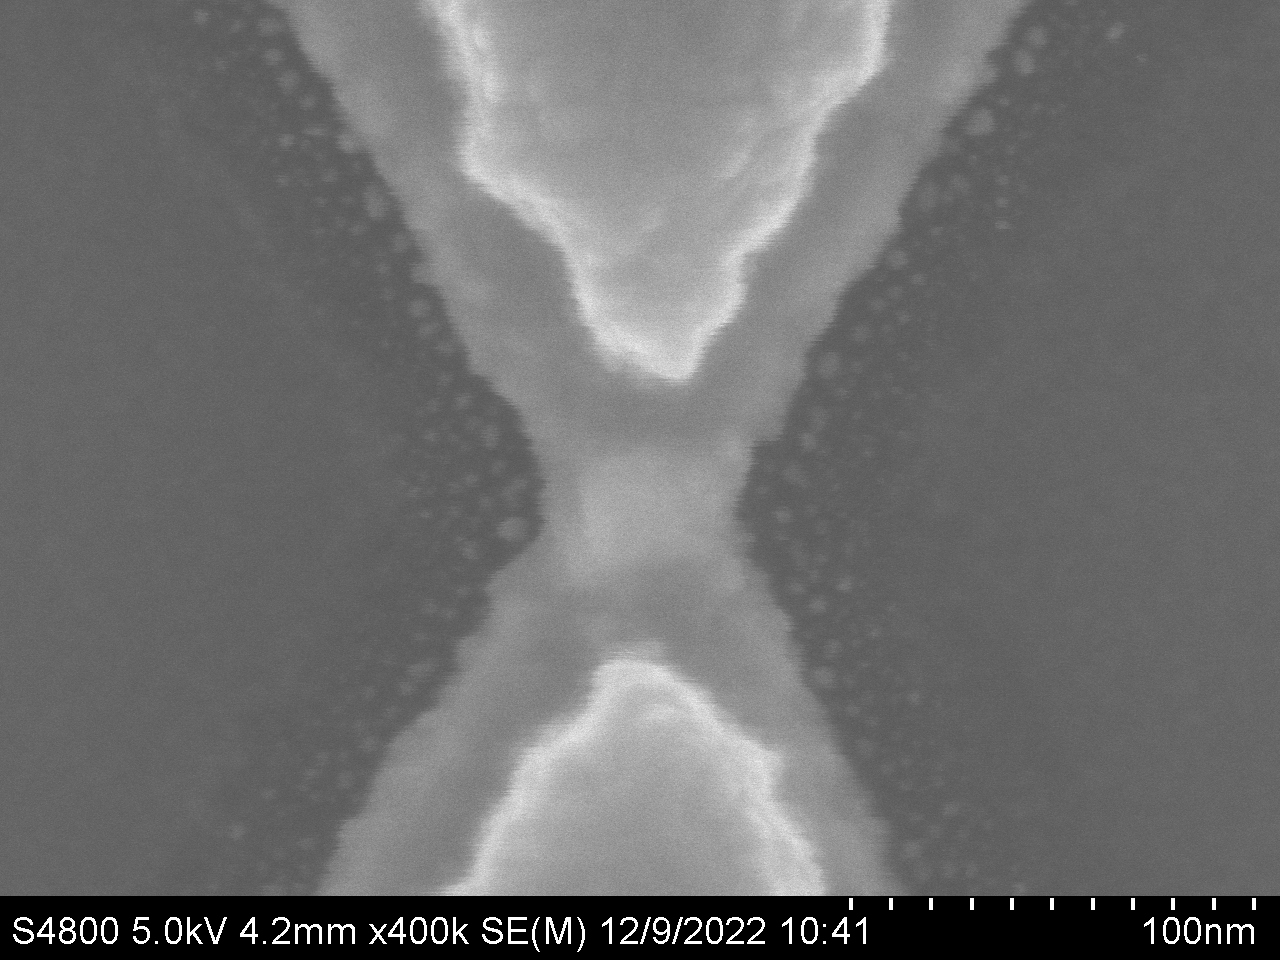
\includegraphics[width=0.32\textwidth]{Appendix_A/A3/A2.png}
         %\caption{A portion of the resist is irradiated with an electron beam in as specified pattern.}
         %\label{c}
     \end{subfigure}
     %\hfill
     \begin{subfigure}[b]{\textwidth}
         \centering
         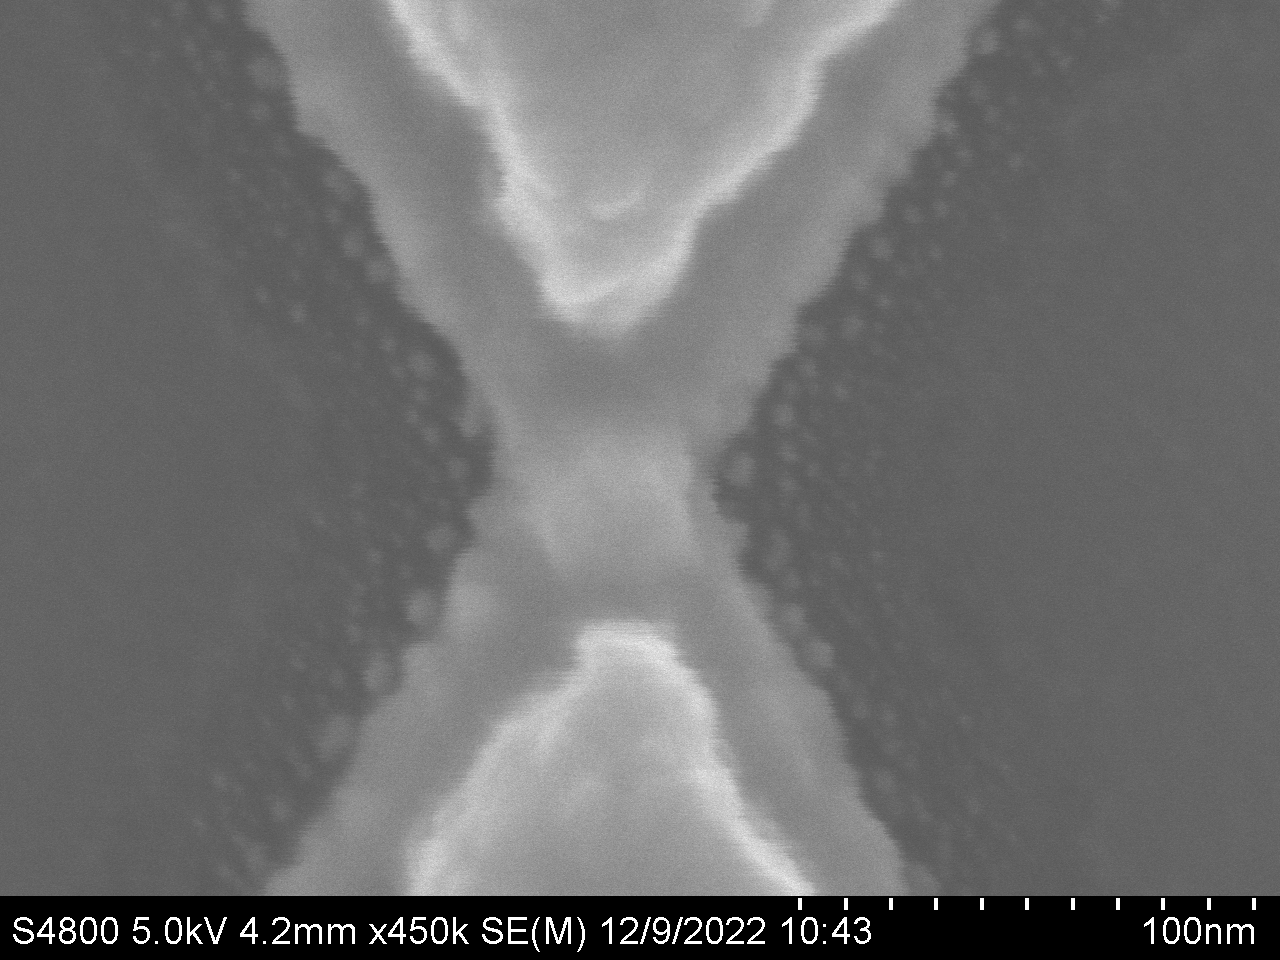
\includegraphics[width=0.32\textwidth]{Appendix_A/A3/A3.png}
         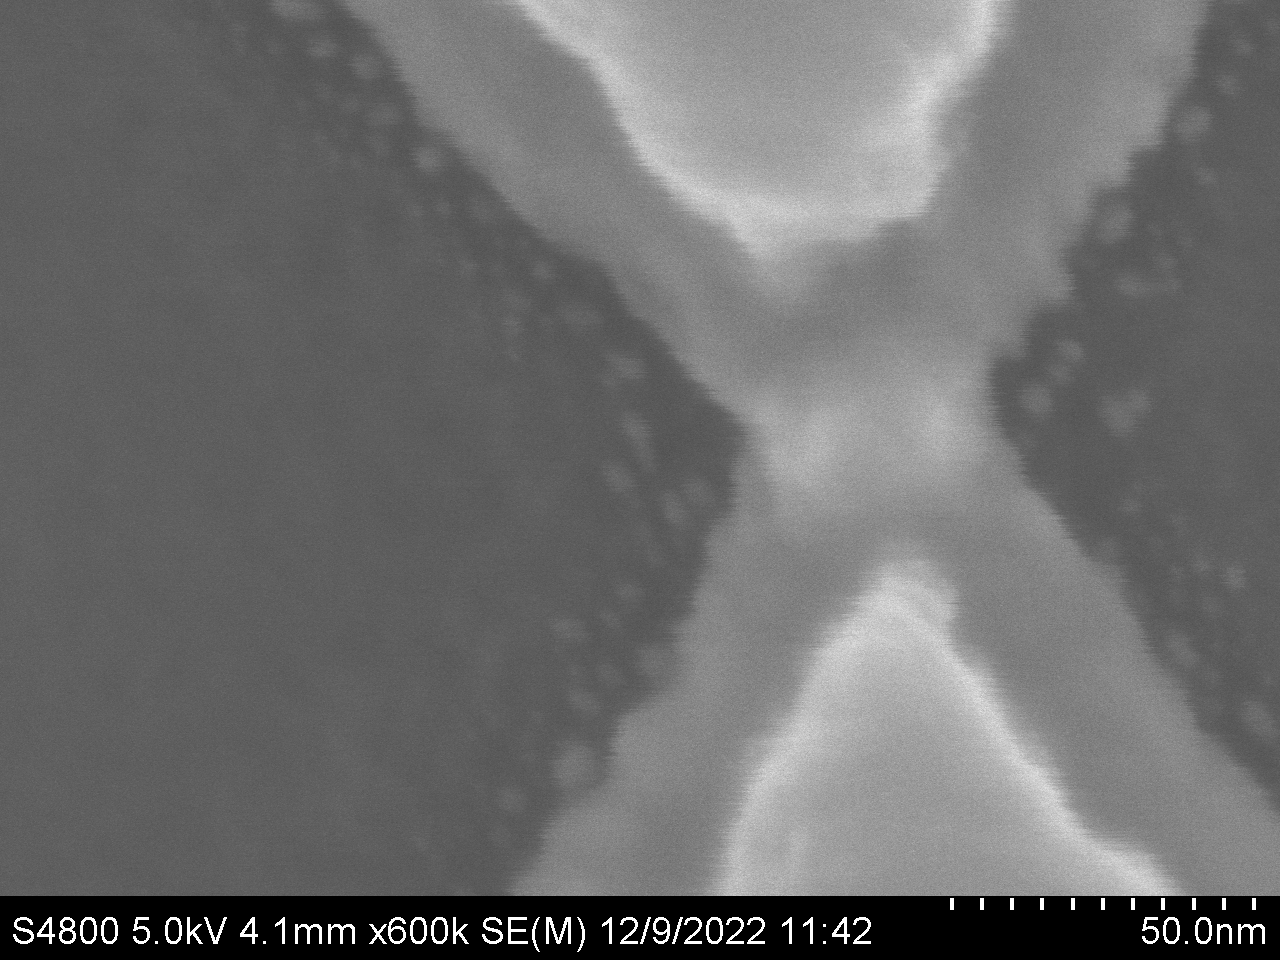
\includegraphics[width=0.32\textwidth]{Appendix_A/A3/B2_zoom.png}
         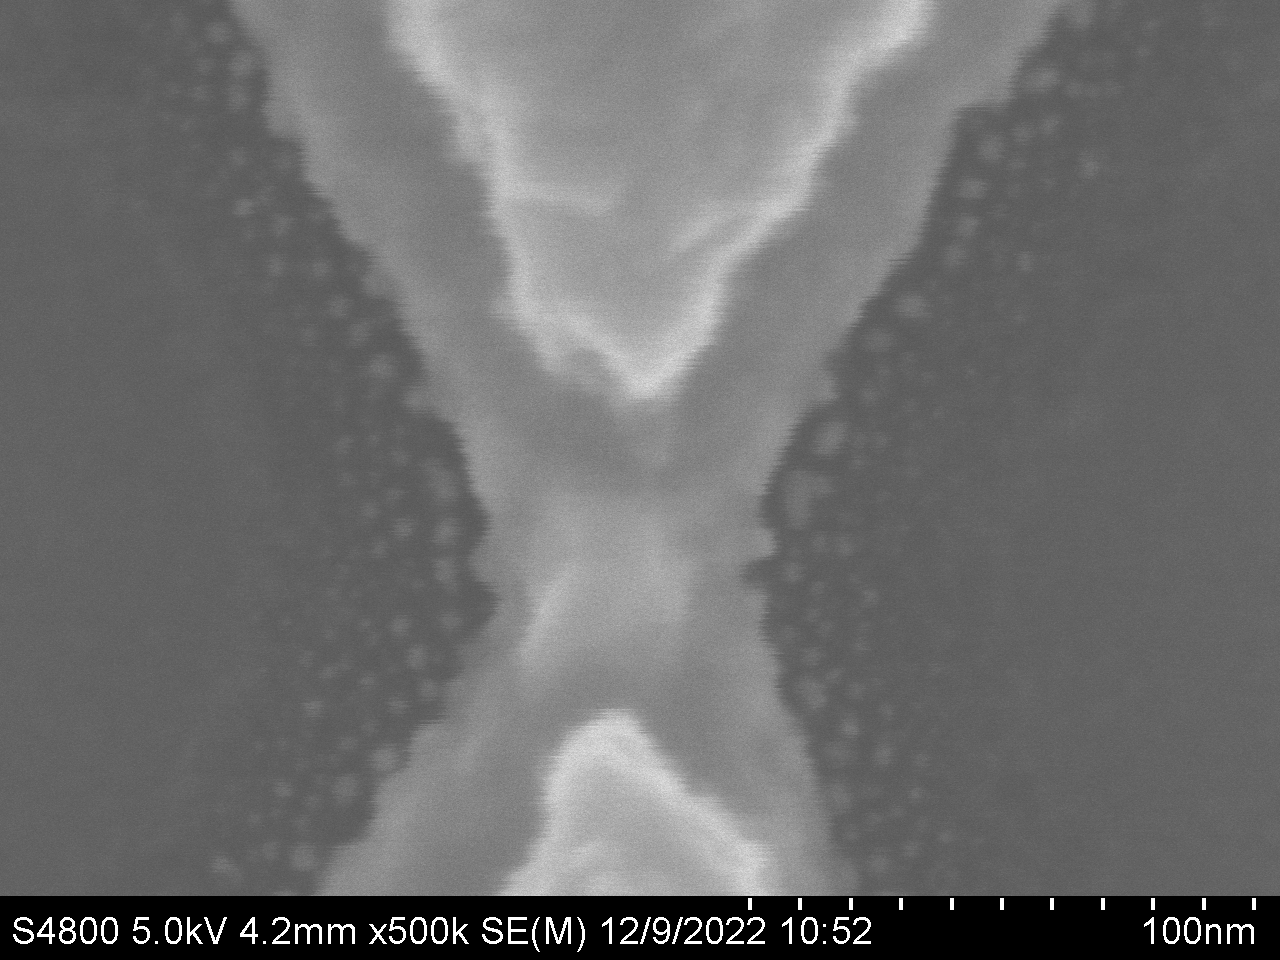
\includegraphics[width=0.32\textwidth]{Appendix_A/A3/A2_2.png}

         %\caption{A portion of the resist is irradiated with an electron beam in as specified pattern.}
         %\label{c}
     \end{subfigure}
        \caption{SEM images of AuNb devices with a 50 nm niobium layer.}
        \label{fig:}
        
\end{figure}

\subsubsection*{A4: AuNb, 60 nm Spacing}
\begin{figure}[H]
     \centering
     \begin{subfigure}[b]{\textwidth}
         \centering
         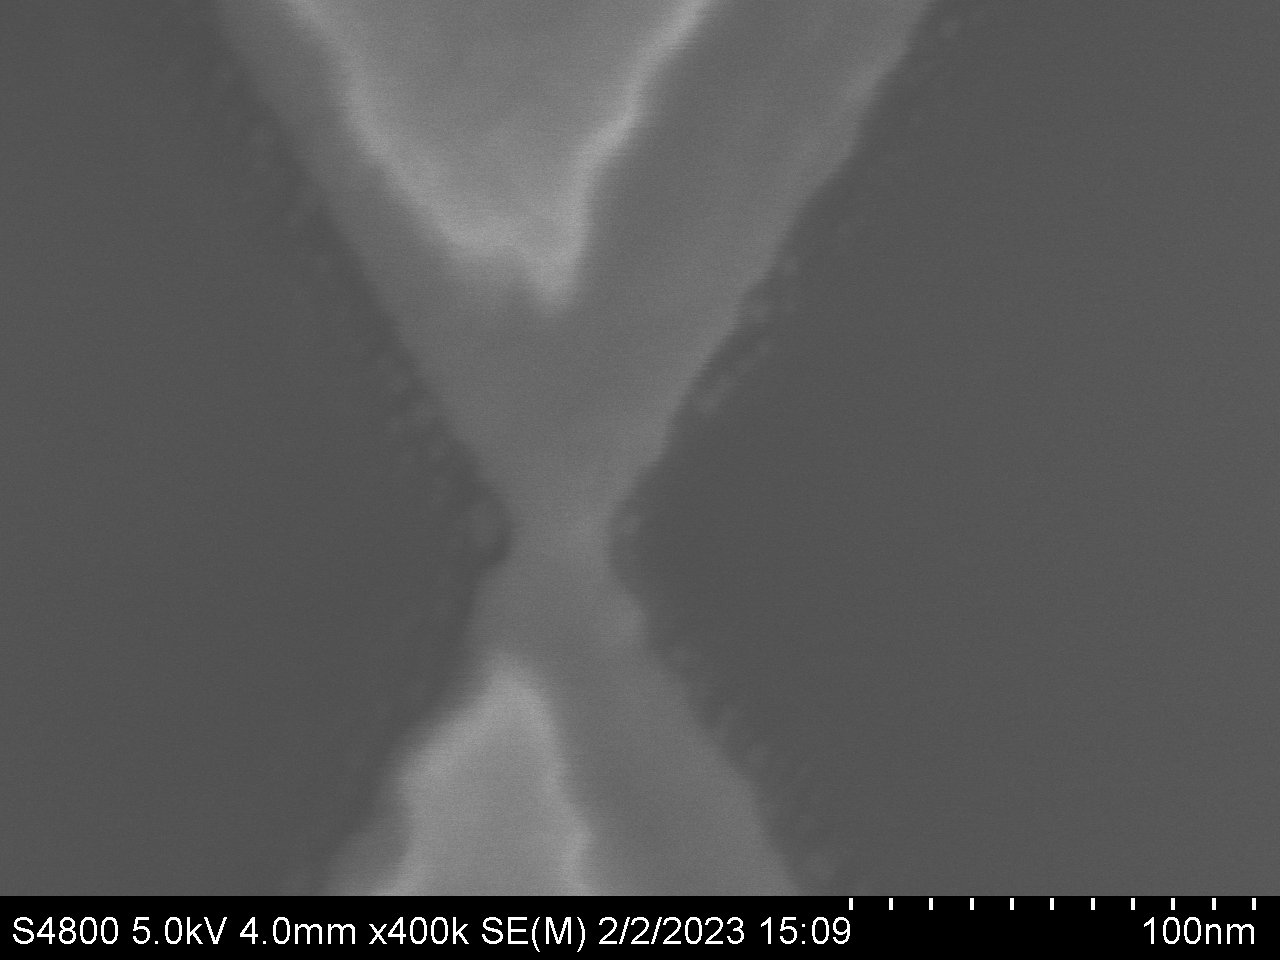
\includegraphics[width=0.32\textwidth]{Appendix_A/A4/60nmsetE1.png}
         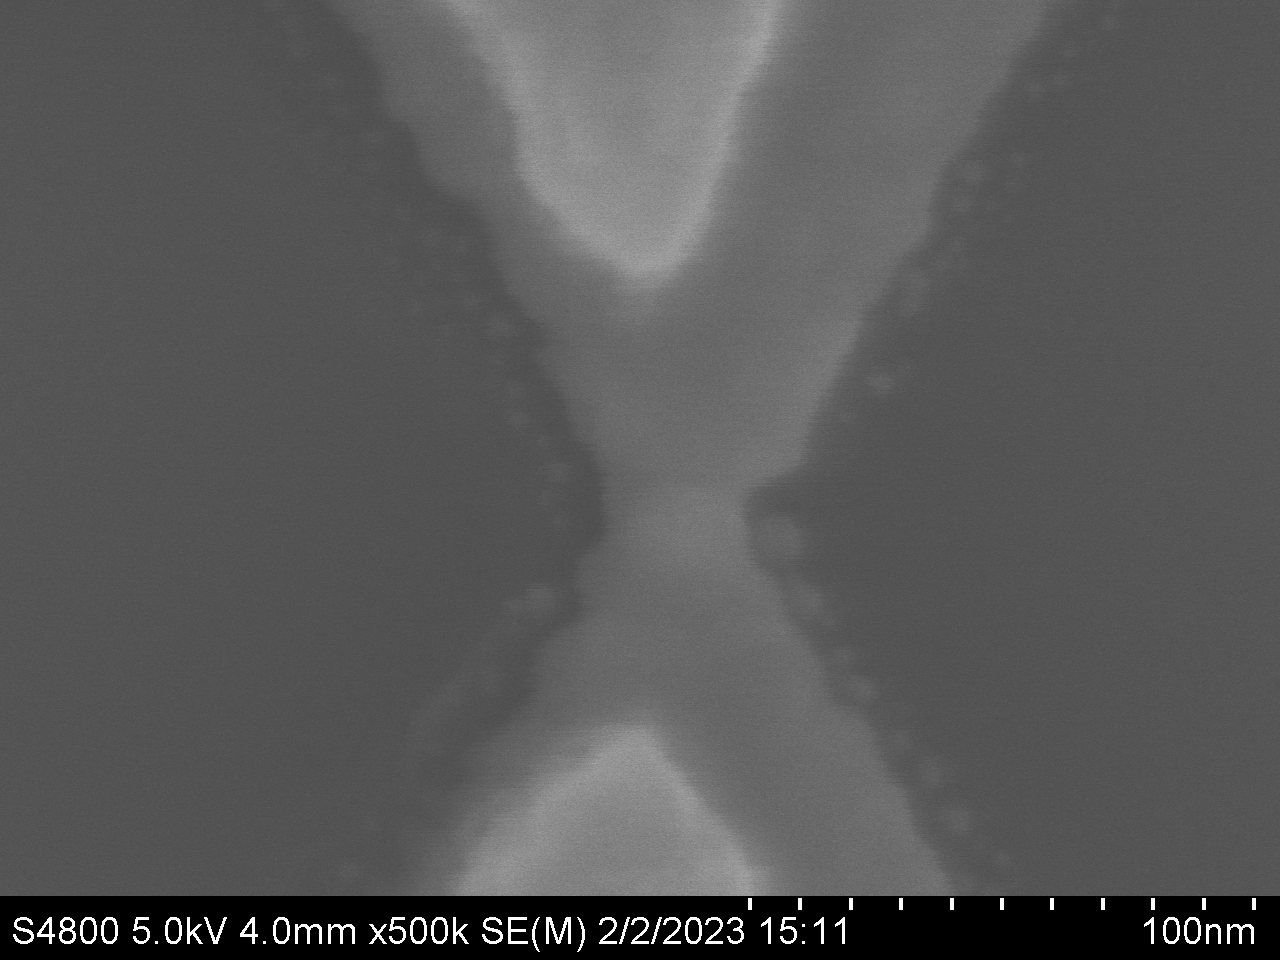
\includegraphics[width=0.32\textwidth]{Appendix_A/A4/60nmsetE2.png}
         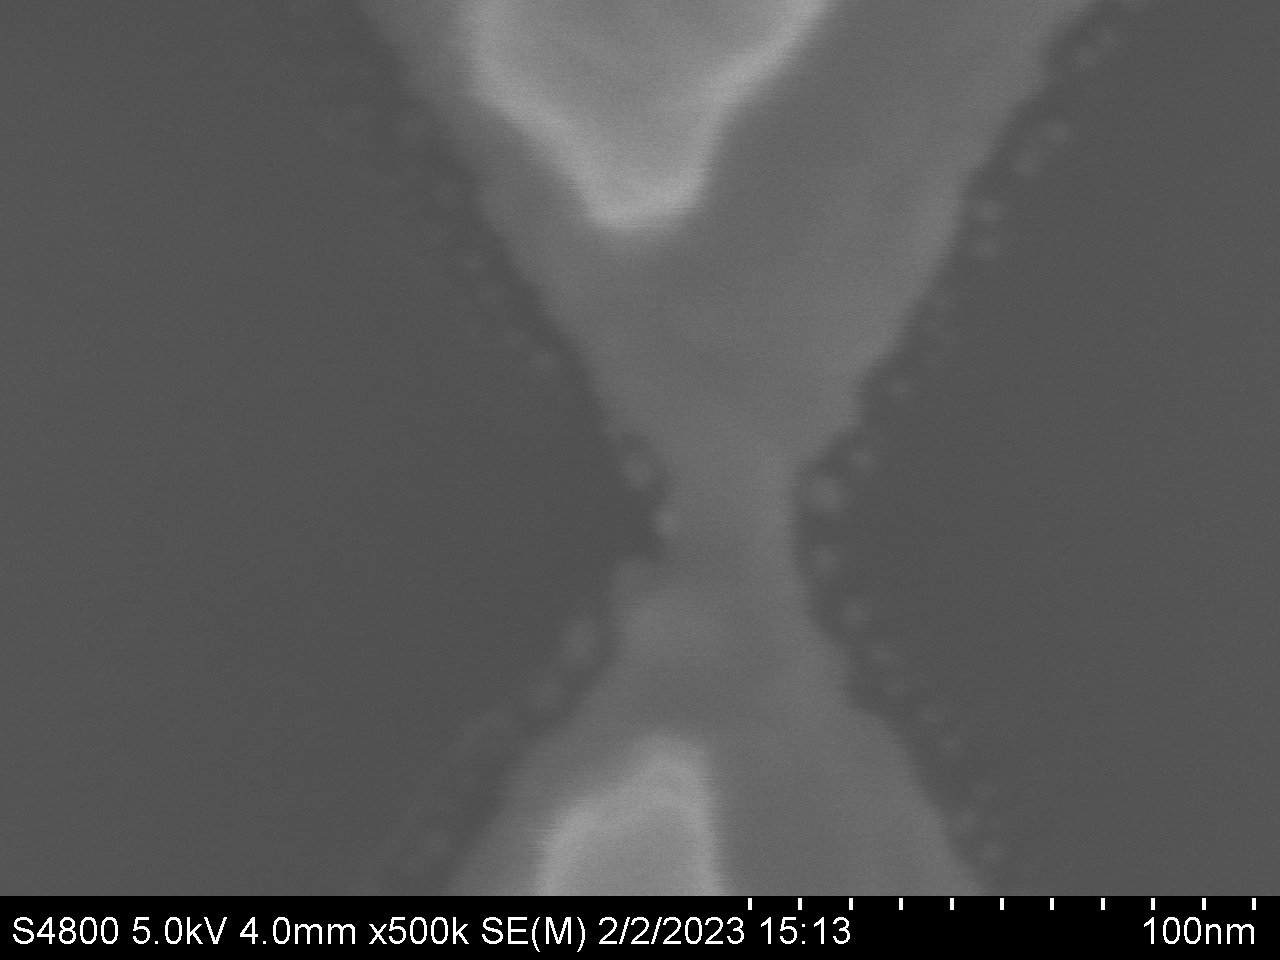
\includegraphics[width=0.32\textwidth]{Appendix_A/A4/60nmsetE3.png}
         %\caption{A portion of the resist is irradiated with an electron beam in as specified pattern.}
         %\label{c}
     \end{subfigure}
     %\hfill
     \begin{subfigure}[b]{\textwidth}
         \centering
         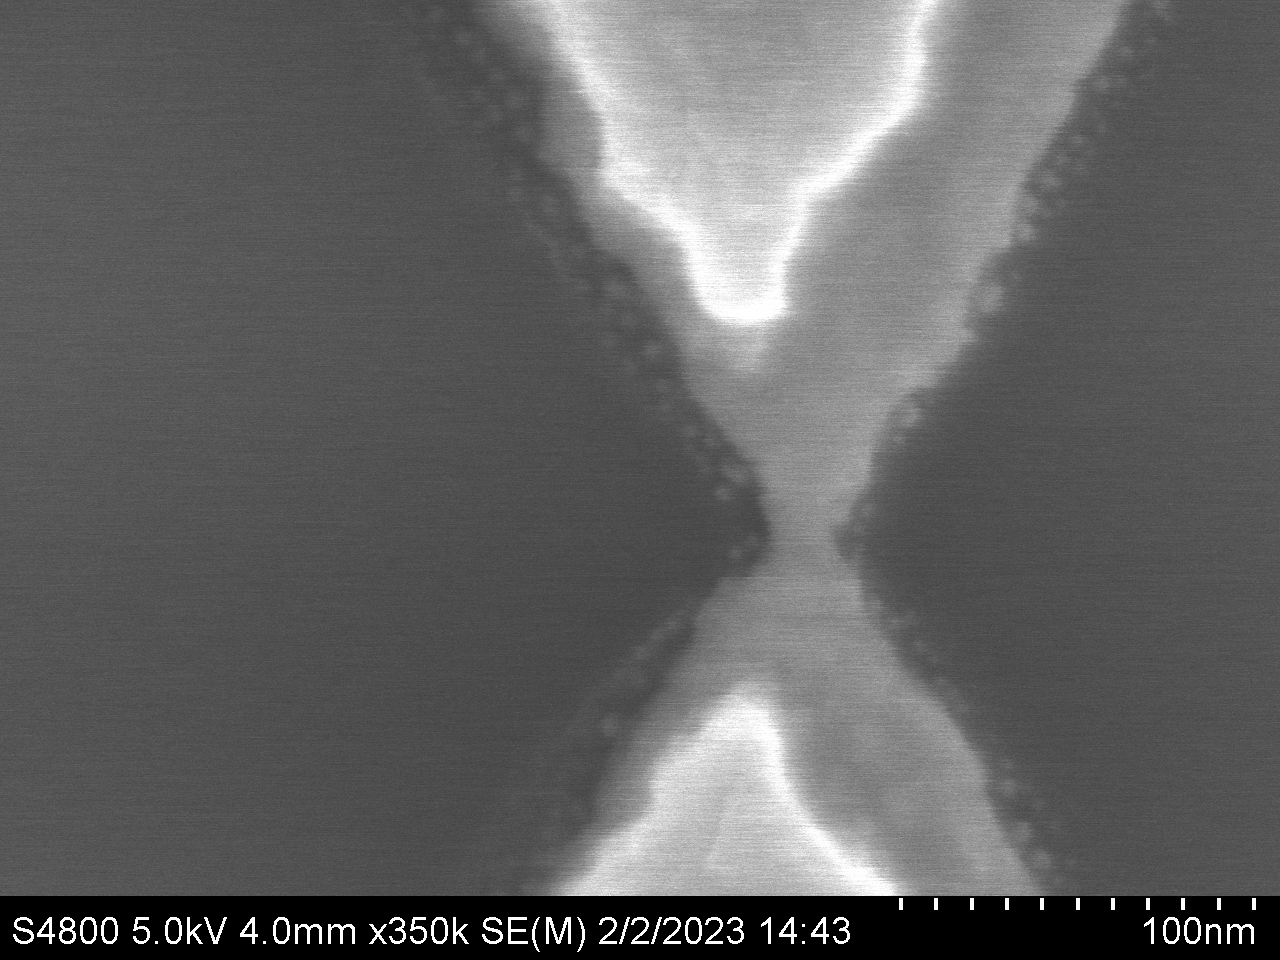
\includegraphics[width=0.32\textwidth]{Appendix_A/A4/variousb360nm.png}
         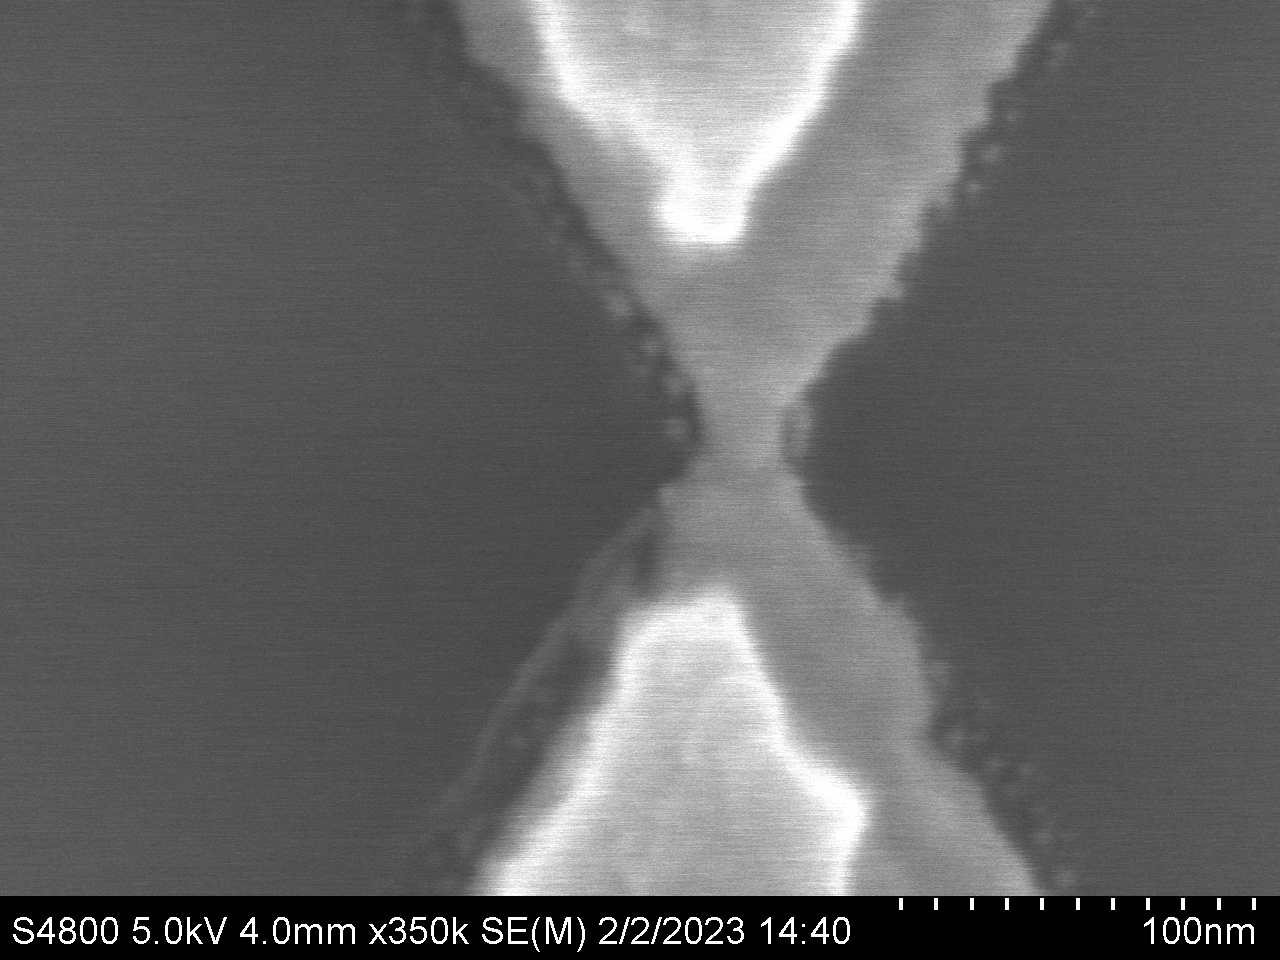
\includegraphics[width=0.32\textwidth]{Appendix_A/A4/variousB160nm.png}
         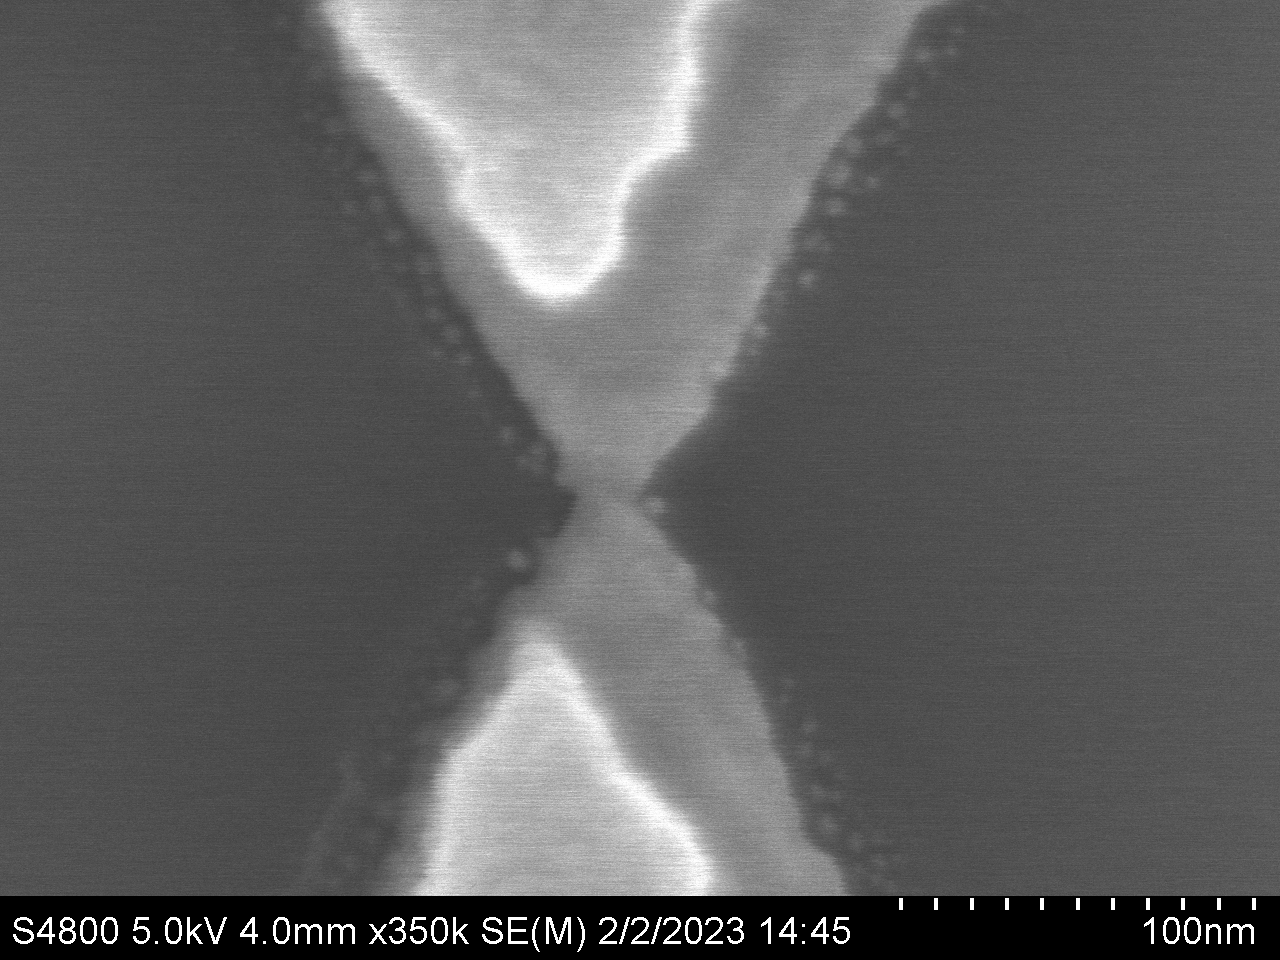
\includegraphics[width=0.32\textwidth]{Appendix_A/A4/variousb460nm.png}
         %\caption{A portion of the resist is irradiated with an electron beam in as specified pattern.}
         %\label{c}
     \end{subfigure}
        \caption{SEM images of AuNb devices with 60 nm spacing.}
        \label{fig:}
        
\end{figure}

\subsection{B: VI Measurement Results}
\subsubsection*{B1: PdNb}

\begin{figure}[H]
     \centering
     \begin{subfigure}[b]{\textwidth}
         \centering
         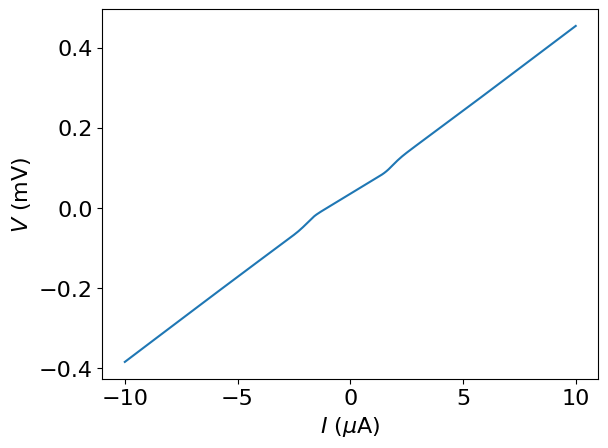
\includegraphics[width=0.32\textwidth]{Appendix_B/B1/VI_PdNb_numid2.png}
         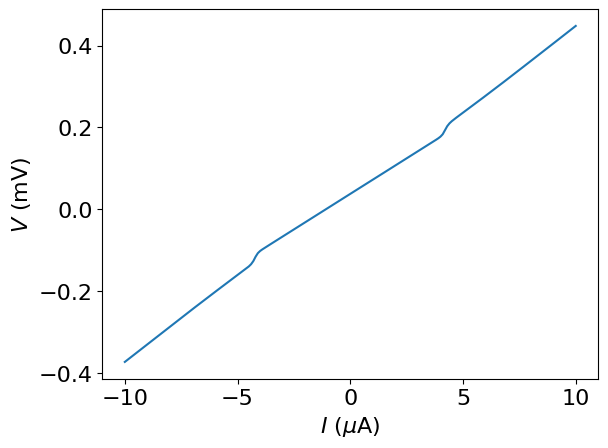
\includegraphics[width=0.32\textwidth]{Appendix_B/B1/VI_PdNb_numid3.png}
         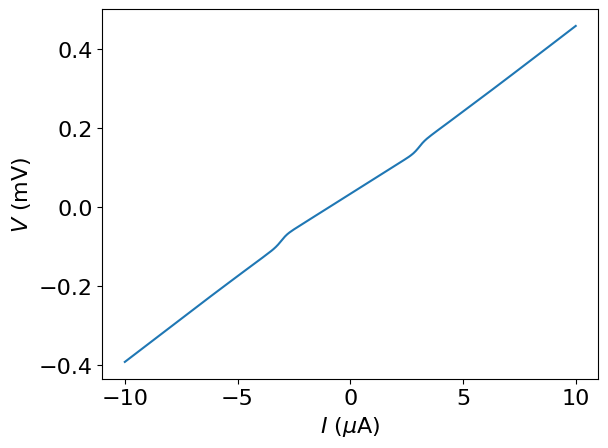
\includegraphics[width=0.32\textwidth]{Appendix_B/B1/VI_PdNb_numid4.png}
         %\caption{A portion of the resist is irradiated with an electron beam in as specified pattern.}
         %\label{c}
     \end{subfigure}
     %\hfill
     \begin{subfigure}[b]{\textwidth}
         \centering
         \includegraphics[width=0.32\textwidth]{Appendix_B/B1/dVdI_PdNb_numid2.png}
         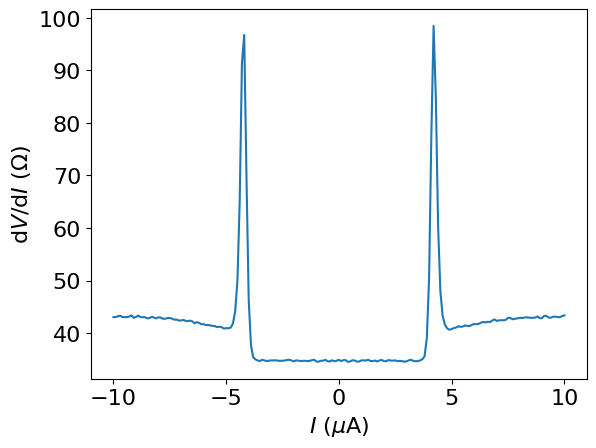
\includegraphics[width=0.32\textwidth]{Appendix_B/B1/dVdI_PdNb_numid3.png}
         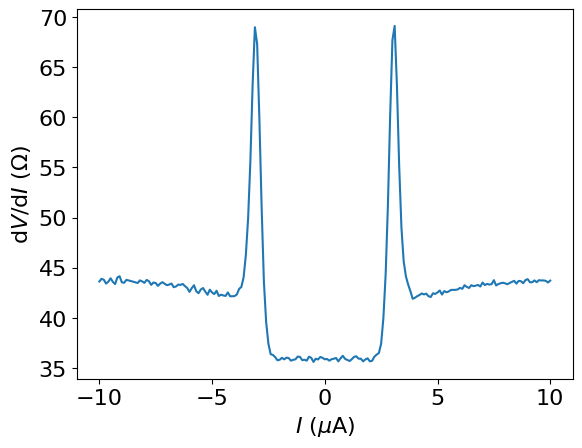
\includegraphics[width=0.32\textwidth]{Appendix_B/B1/dVdI_PdNb_numid4.png}
         %\caption{A portion of the resist is irradiated with an electron beam in as specified pattern.}
         %\label{c}
     \end{subfigure}
        \caption{VI measurements and their derivatives, measured at 1.2 K}
        \label{fig:}
        
\end{figure}

\subsubsection*{B2: AuNb, 100 nm Nb}

\begin{figure}[H]
     \centering
     \begin{subfigure}[b]{\textwidth}
         \centering
         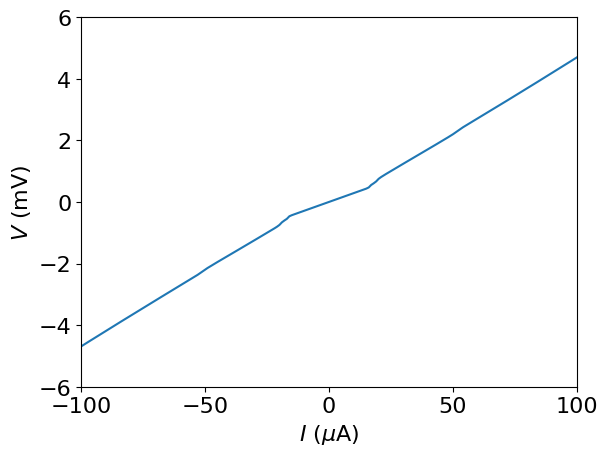
\includegraphics[width=0.32\textwidth]{Appendix_B/B2/VI_AuNbV2_numid19.png}
         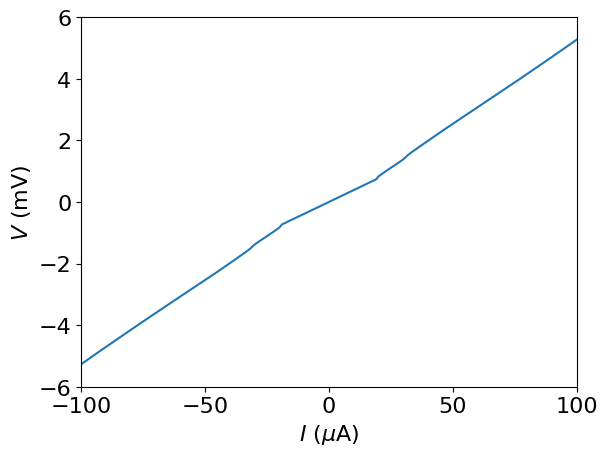
\includegraphics[width=0.32\textwidth]{Appendix_B/B2/VI_AuNbV2_numid20.png}
         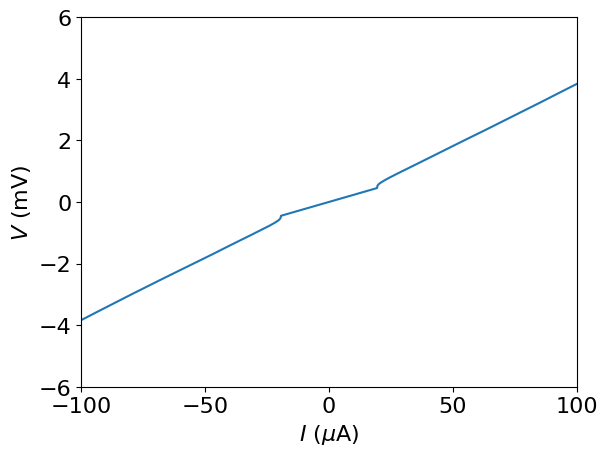
\includegraphics[width=0.32\textwidth]{Appendix_B/B2/VI_AuNbV2_numid26.png}
         %\caption{A portion of the resist is irradiated with an electron beam in as specified pattern.}
         %\label{c}
     \end{subfigure}
     %\hfill
     \begin{subfigure}[b]{\textwidth}
         \centering
         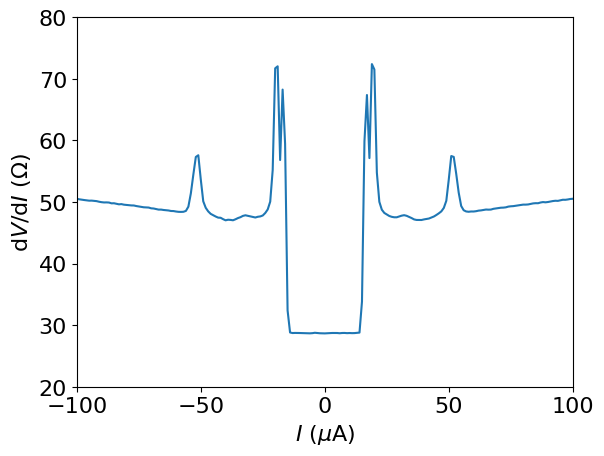
\includegraphics[width=0.32\textwidth]{Appendix_B/B2/dVdI_AuNbV2_numid19.png}
         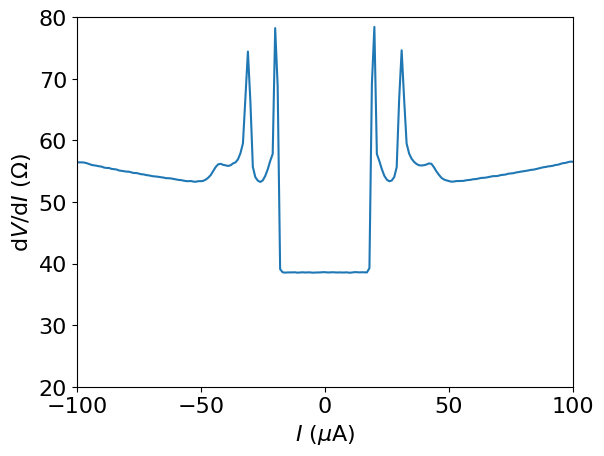
\includegraphics[width=0.32\textwidth]{Appendix_B/B2/dVdI_AuNbV2_numid20.png}
         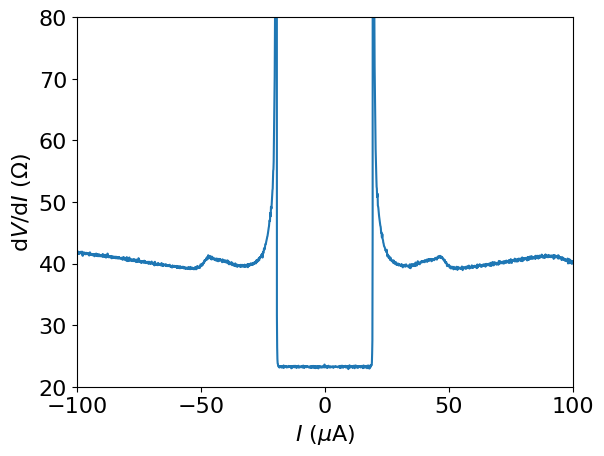
\includegraphics[width=0.32\textwidth]{Appendix_B/B2/dVdI_AuNbV2_numid26.png}
         %\caption{A portion of the resist is irradiated with an electron beam in as specified pattern.}
         %\label{c}
     \end{subfigure}
        \caption{VI measurements and their derivatives, measured at 1.8 K}
        \label{fig:}
        
\end{figure}

\subsubsection*{B3: AuNb, 50 nm Nb}

\begin{figure}[H]
     \centering
     \begin{subfigure}[b]{\textwidth}
         \centering
         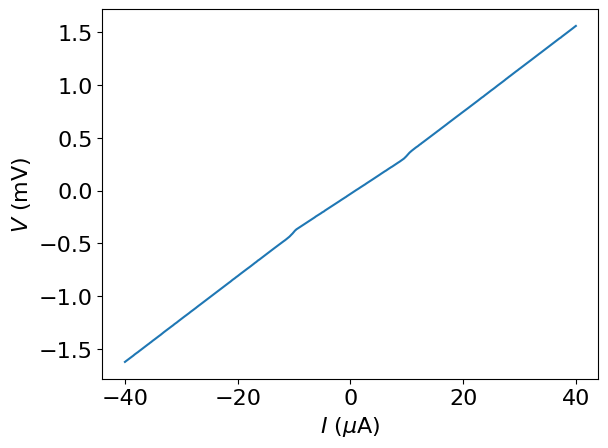
\includegraphics[width=0.32\textwidth]{Appendix_B/B3/VI_AuNbV3DF_numid12.png}
         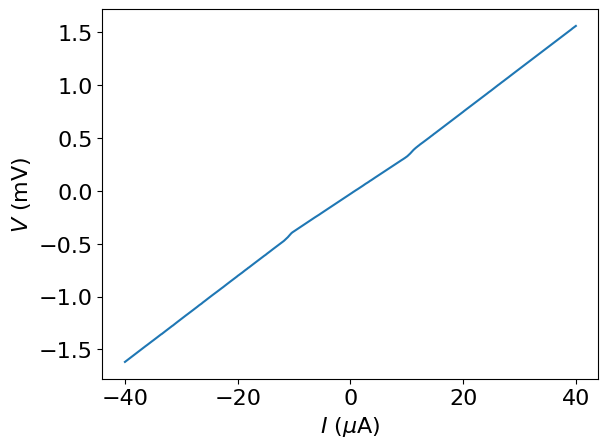
\includegraphics[width=0.32\textwidth]{Appendix_B/B3/VI_AuNbV3DF_numid13.png}
         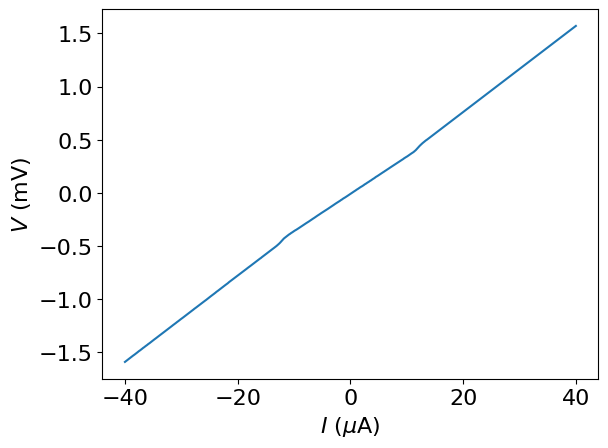
\includegraphics[width=0.32\textwidth]{Appendix_B/B3/VI_AuNbV3DF_numid14.png}
         %\caption{A portion of the resist is irradiated with an electron beam in as specified pattern.}
         %\label{c}
     \end{subfigure}
     %\hfill
     \begin{subfigure}[b]{\textwidth}
         \centering
         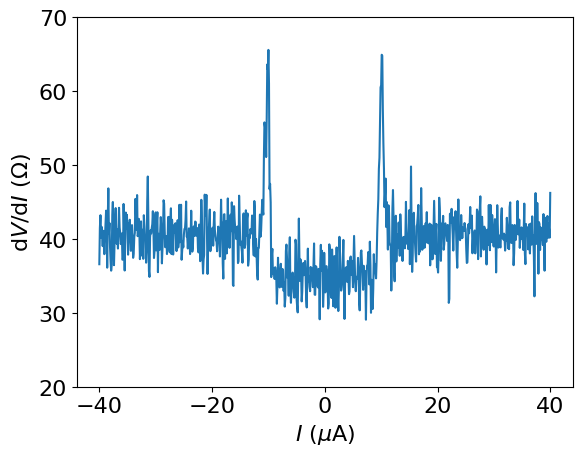
\includegraphics[width=0.32\textwidth]{Appendix_B/B3/dVdI_AuNbV3DF_numid12.png}
         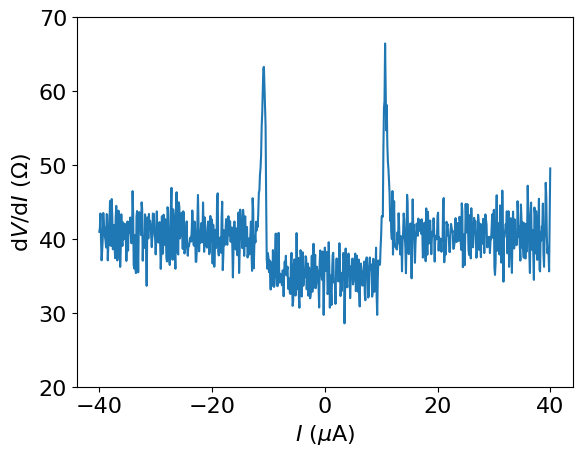
\includegraphics[width=0.32\textwidth]{Appendix_B/B3/dVdI_AuNbV3DF_numid13.png}
         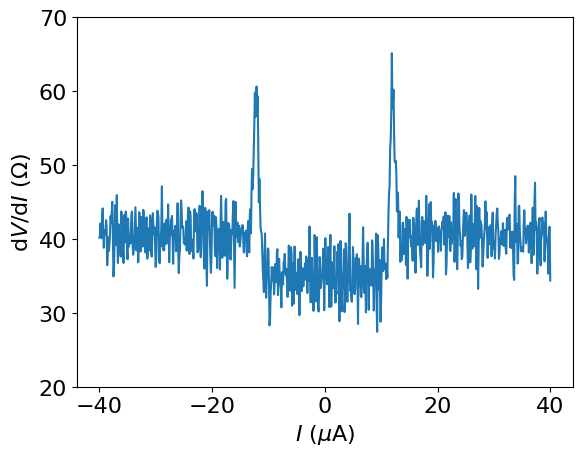
\includegraphics[width=0.32\textwidth]{Appendix_B/B3/dVdI_AuNbV3DF_numid14.png}
         %\caption{A portion of the resist is irradiated with an electron beam in as specified pattern.}
         %\label{c}
     \end{subfigure}
        \caption{VI measurements and their derivatives. The four figures on the left have been measured at 1.9 K, the two on the right at 40 mK.}
        \label{fig:}
        
\end{figure}


\subsubsection*{B4: AuNb, 60 nm Spacing}
\begin{figure}[H]
     \centering
     \begin{subfigure}[b]{\textwidth}
         \centering
         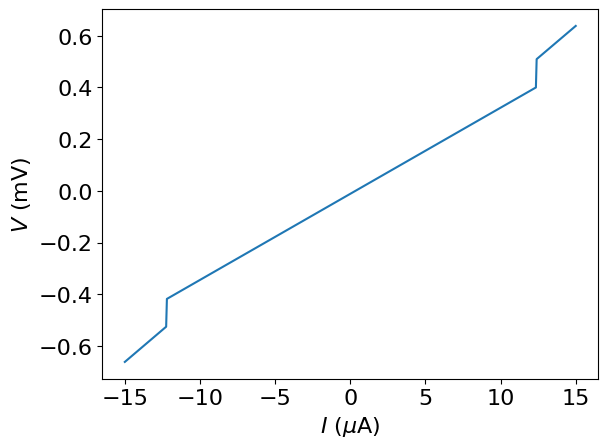
\includegraphics[width=0.32\textwidth]{Appendix_B/B4/VI_AuNb60nm_numid36.png}
         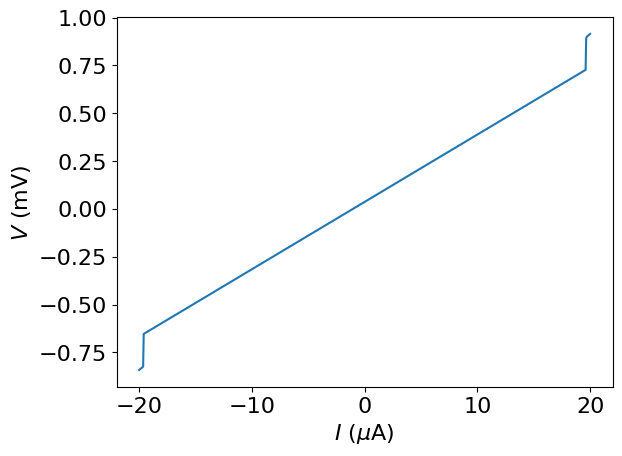
\includegraphics[width=0.32\textwidth]{Appendix_B/B4/VI_AuNb60nm_numid38.png}
         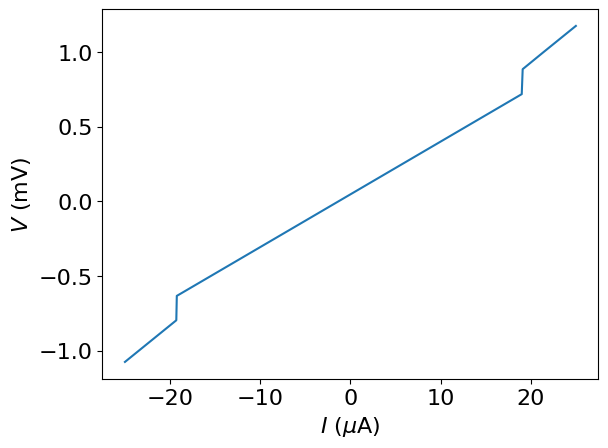
\includegraphics[width=0.32\textwidth]{Appendix_B/B4/VI_AuNb60nm_numid40.png}
         %\caption{A portion of the resist is irradiated with an electron beam in as specified pattern.}
         %\label{c}
     \end{subfigure}
     %\hfill
     \begin{subfigure}[b]{\textwidth}
         \centering
         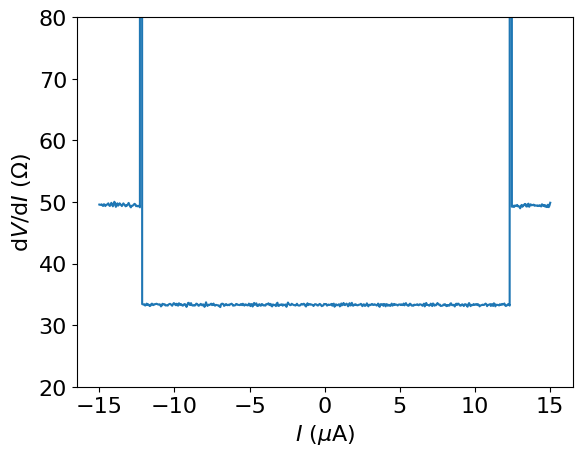
\includegraphics[width=0.32\textwidth]{Appendix_B/B4/dVdI_AuNb60nm_numid36.png}
         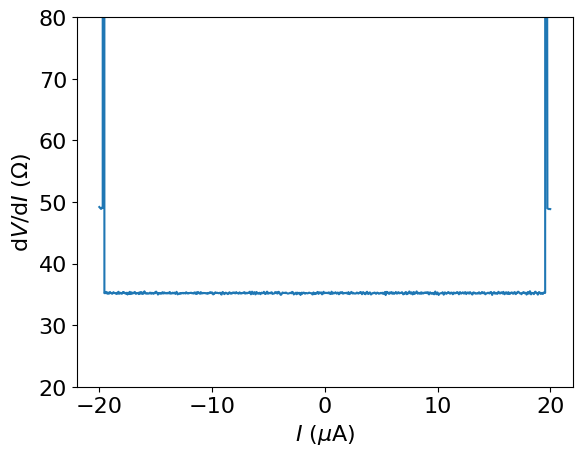
\includegraphics[width=0.32\textwidth]{Appendix_B/B4/dVdI_AuNb60nm_numid38.png}
         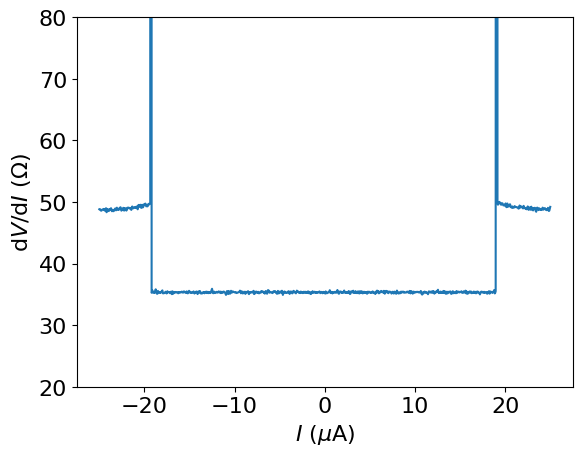
\includegraphics[width=0.32\textwidth]{Appendix_B/B4/dVdI_AuNb60nm_numid40.png}
         %\caption{A portion of the resist is irradiated with an electron beam in as specified pattern.}
         %\label{c}
     \end{subfigure}
        \caption{VI measurements and their derivatives, measured at 30 mK. Current has been swept from 0 in the positive direction, and then from 0 in the negative direction.}
        \label{fig:}
        
\end{figure}


\subsection{C: VIT Measurement Results}
\subsubsection*{C1: PdNb}
\begin{figure}[H]
     \centering
     \begin{subfigure}[b]{\textwidth}
         \centering
         \includegraphics[width=0.32\textwidth]{Appendix_C/C1/PdNb_VIT.png}
         \includegraphics[width=0.32\textwidth]{Appendix_C/C1/PdNb_dVdIT.png}
         %\caption{A portion of the resist is irradiated with an electron beam in as specified pattern.}
         %\label{c}
     \end{subfigure}
        \caption{VIT measurement.}
        \label{fig:}
        
\end{figure}

\subsubsection*{C2: AuNb, 100 nm Nb}
\begin{figure}[H]
     \centering
     \begin{subfigure}[b]{\textwidth}
         \centering
         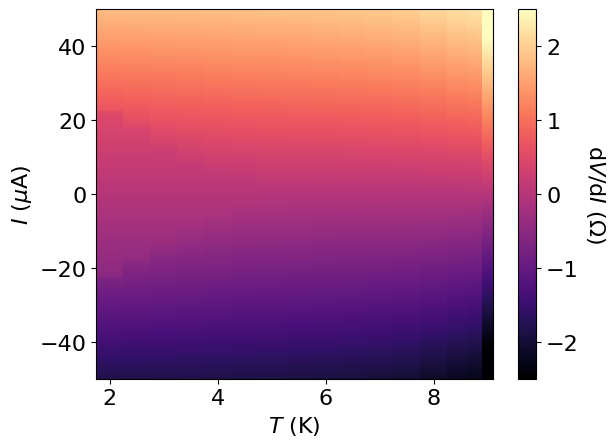
\includegraphics[width=0.32\textwidth]{Appendix_C/C2/AuNbV2_VIT.png}
         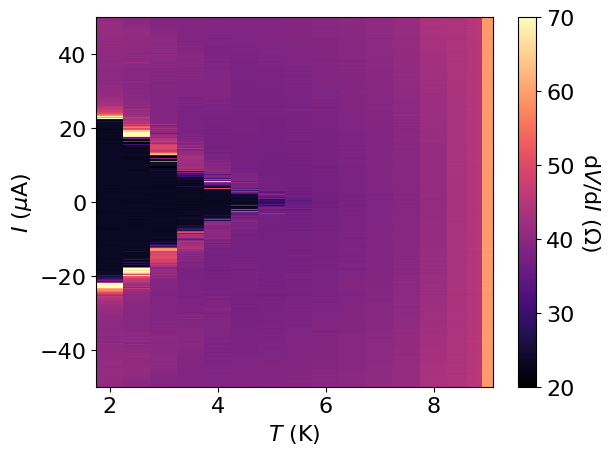
\includegraphics[width=0.32\textwidth]{Appendix_C/C2/AuNbV2_dVdIT.png}
         %\caption{A portion of the resist is irradiated with an electron beam in as specified pattern.}
         %\label{c}
     \end{subfigure}
        \caption{VIT measurement.}
        \label{fig:}
        
\end{figure}

\subsubsection*{C3: AuNb, 50 nm Nb}

\begin{figure}[H]
     \centering
     \begin{subfigure}[b]{\textwidth}
         \centering
         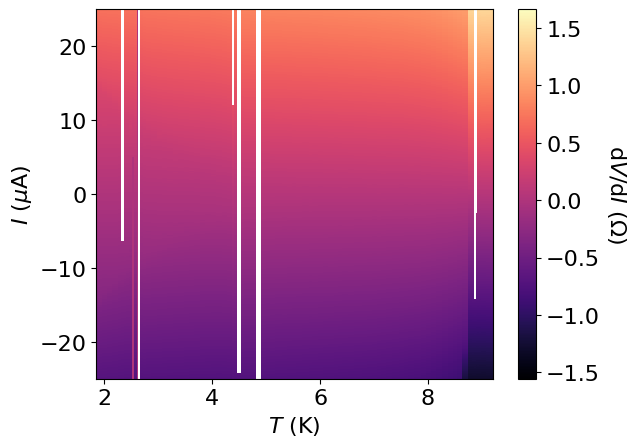
\includegraphics[width=0.32\textwidth]{Appendix_C/C3/AuNbV3_VIT.png}
         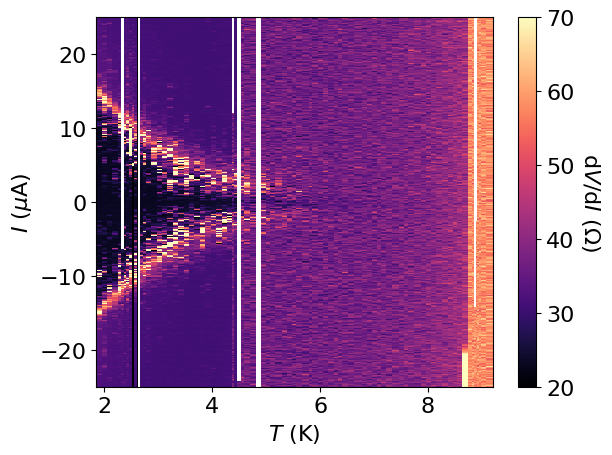
\includegraphics[width=0.32\textwidth]{Appendix_C/C3/AuNbV3_dVdIT.png}
         %\caption{A portion of the resist is irradiated with an electron beam in as specified pattern.}
         %\label{c}
     \end{subfigure}
     %\hfill
     \begin{subfigure}[b]{\textwidth}
         \centering
         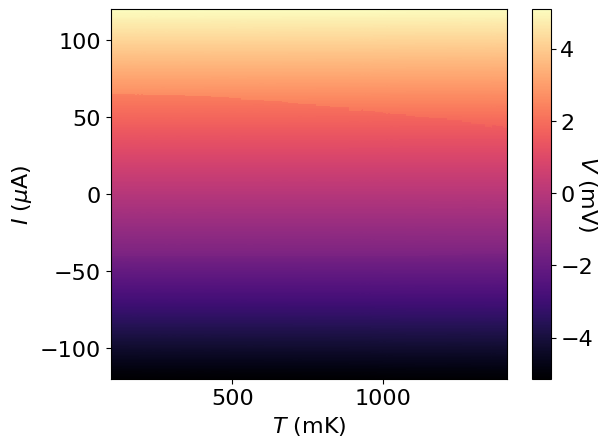
\includegraphics[width=0.32\textwidth]{Appendix_C/C3/AuNbV3DF_VIT.png}
         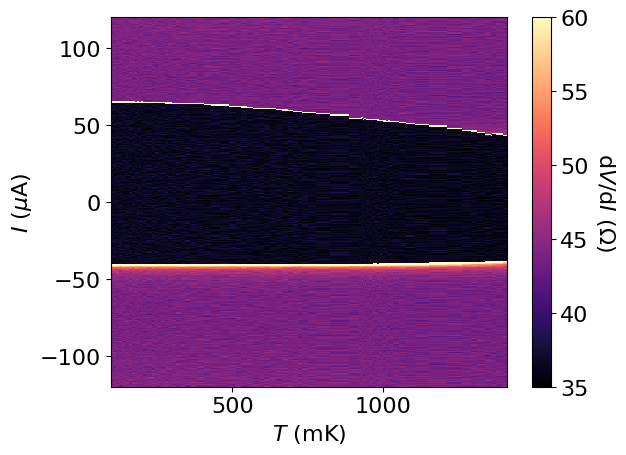
\includegraphics[width=0.32\textwidth]{Appendix_C/C3/AuNbV3DF_dVdIT.png}
         %\caption{A portion of the resist is irradiated with an electron beam in as specified pattern.}
         %\label{c}
     \end{subfigure}
        \caption{VIT measurements. Top: Dip-Stick, higher T range. Bottom: Dilution Fridge, lower T range. Different devices made with the same fabrication parameters.}
        \label{fig:}
        
\end{figure}

\subsubsection*{C4: AuNb, 60 nm Spacing}
\begin{figure}[H]
     \centering
     \begin{subfigure}[b]{\textwidth}
         \centering
         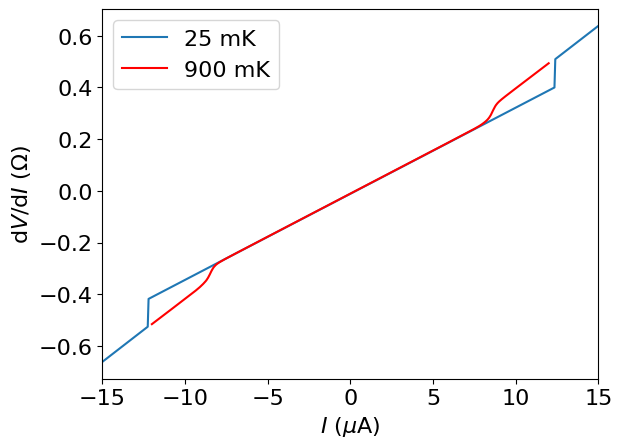
\includegraphics[width=0.32\textwidth]{Appendix_C/C4/AuNb60nm_VIT_A1.png}
         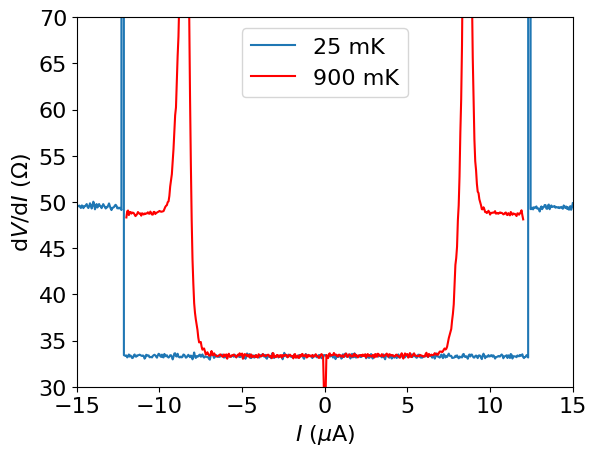
\includegraphics[width=0.32\textwidth]{Appendix_C/C4/AuNb60nm_dVdIT_A1.png}
         %\caption{A portion of the resist is irradiated with an electron beam in as specified pattern.}
         %\label{c}
     \end{subfigure}
     %\hfill
     \begin{subfigure}[b]{\textwidth}
         \centering
         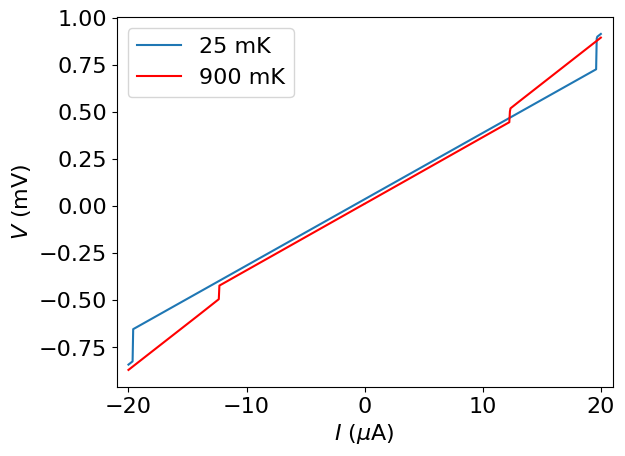
\includegraphics[width=0.32\textwidth]{Appendix_C/C4/AuNb60nm_VIT_A6.png}
         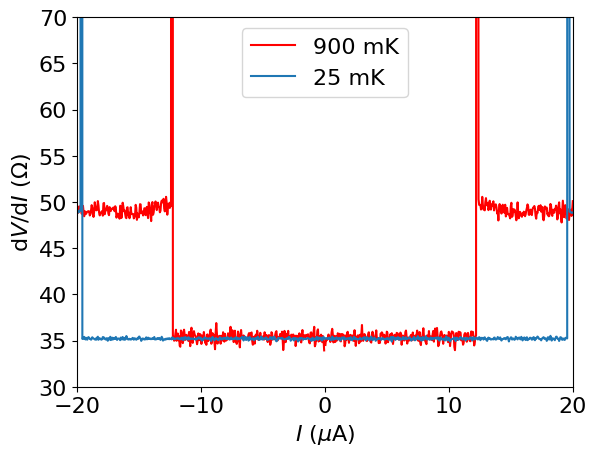
\includegraphics[width=0.32\textwidth]{Appendix_C/C4/AuNb60nm_dVdIT_A6.png}
         %\caption{A portion of the resist is irradiated with an electron beam in as specified pattern.}
         %\label{c}
     \end{subfigure}
        \caption{Two sets of VI measurements of the same device, taken at two different temperatures.}
        \label{fig:}

\end{figure}

\subsection{D: BVI Measurement Results}
\subsubsection*{D1: PdNb}
\subsubsection*{Z Direction, High Field}


\begin{figure}[H]
     \centering
     \begin{subfigure}[b]{\textwidth}
         \centering
         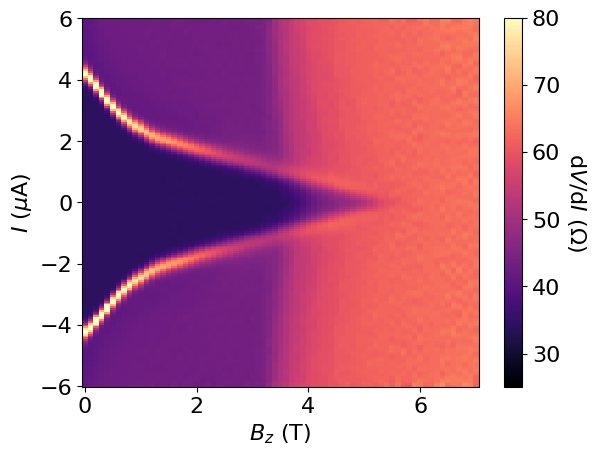
\includegraphics[width=0.32\textwidth]{dVdIBZ_36.png}
         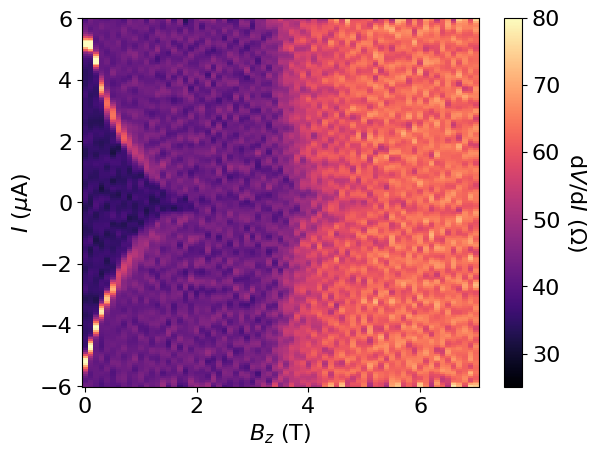
\includegraphics[width=0.32\textwidth]{dVdIBZ_43.png}
         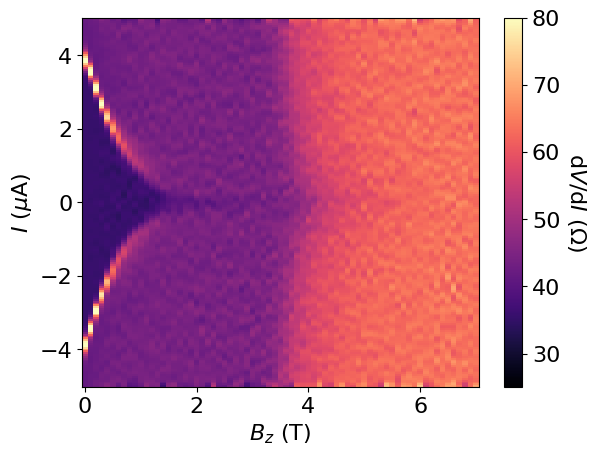
\includegraphics[width=0.32\textwidth]{dVdIBZ_57.png}
         %\caption{A portion of the resist is irradiated with an electron beam in as specified pattern.}
         %\label{c}
     \end{subfigure}
	 \caption{Out of plane BVI measurements.}
     \label{fig:}
        
\end{figure}

\subsubsection*{X,Y,Z directions, Low field}

\begin{figure}[H]
     \centering
     \begin{subfigure}[b]{\textwidth}
         \centering
         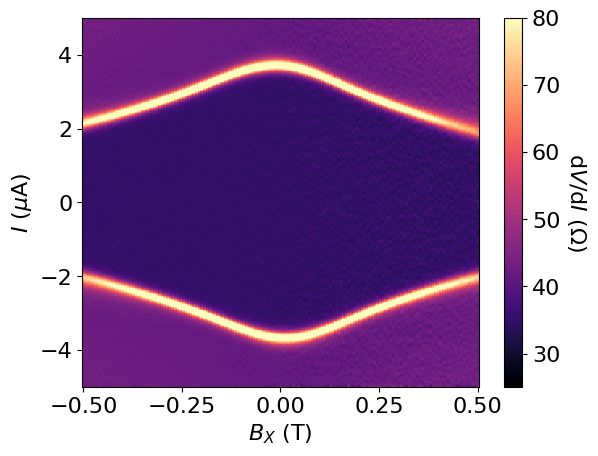
\includegraphics[width=0.32\textwidth]{dVdIBX_64.png}
         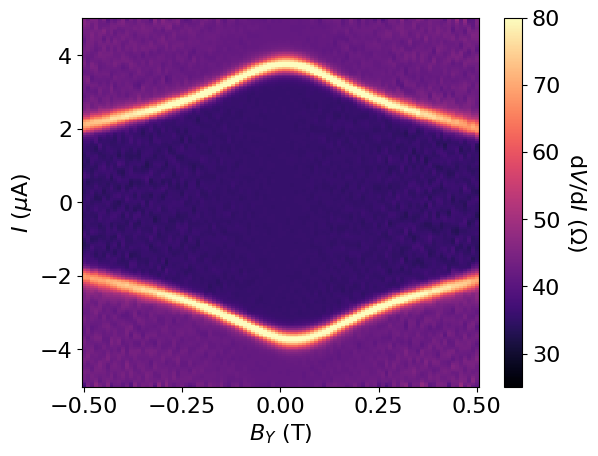
\includegraphics[width=0.32\textwidth]{dVdIBY_63.png}
         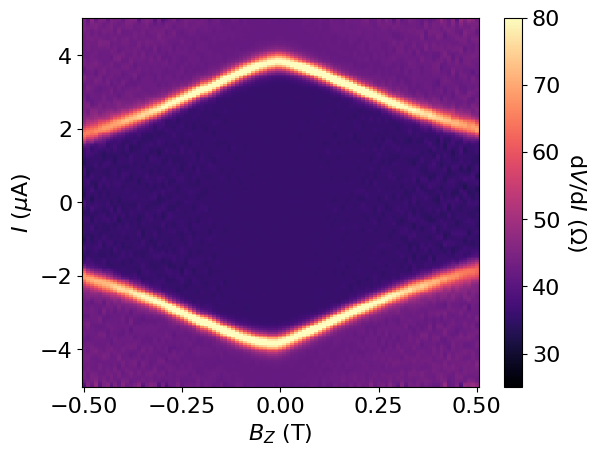
\includegraphics[width=0.32\textwidth]{dVdIBZ_61.png}
         %\caption{A portion of the resist is irradiated with an electron beam in as specified pattern.}
         %\label{c}
     \end{subfigure}
	 \caption{BVI measurements in the X, Y and Z directions.}
     \label{fig:}
        
\end{figure}

\subsubsection*{$\phi$, $\theta$ Sweep}

\begin{figure}[H]
     \centering
     \begin{subfigure}[b]{\textwidth}
         \centering
         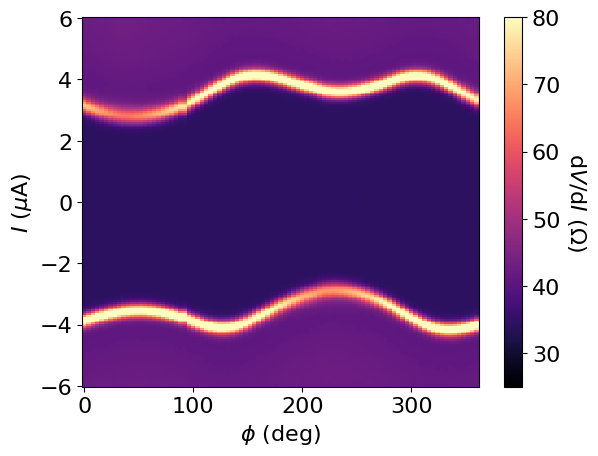
\includegraphics[width=0.32\textwidth]{dVdIphisweep_49.png}
         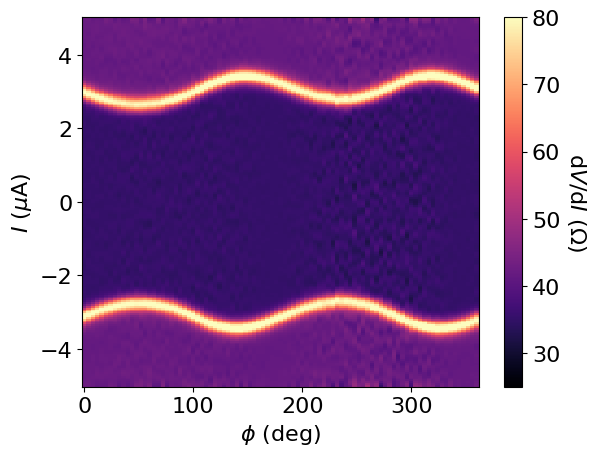
\includegraphics[width=0.32\textwidth]{dVdIphisweep_68.png}
         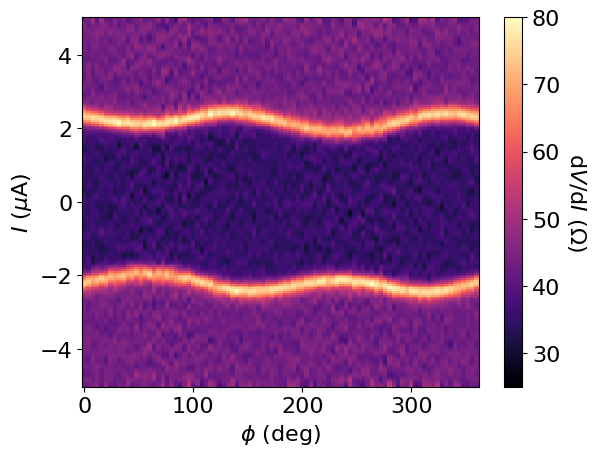
\includegraphics[width=0.32\textwidth]{dVdIphisweep_69.png}
         %\caption{A portion of the resist is irradiated with an electron beam in as specified pattern.}
         %\label{c}
     \end{subfigure}
     %\hfill
     \begin{subfigure}[b]{\textwidth}
         \centering
         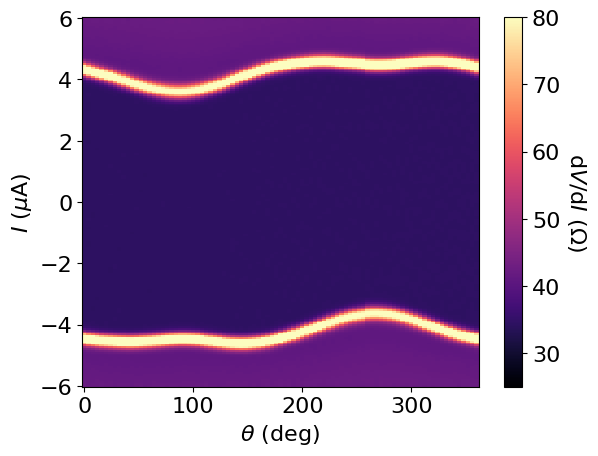
\includegraphics[width=0.32\textwidth]{dVdIthetasweep_55.png}
         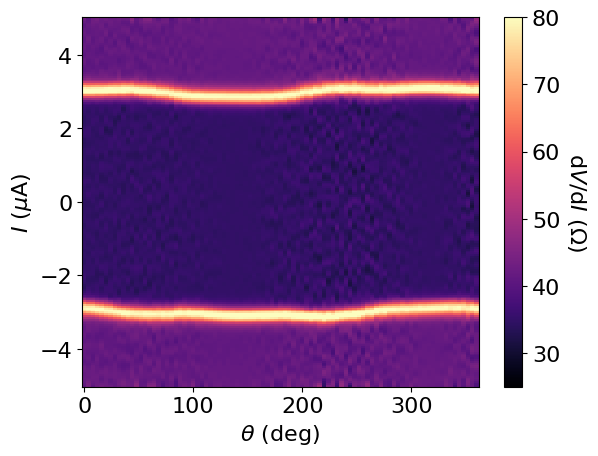
\includegraphics[width=0.32\textwidth]{dVdIthetasweep_71.png}
         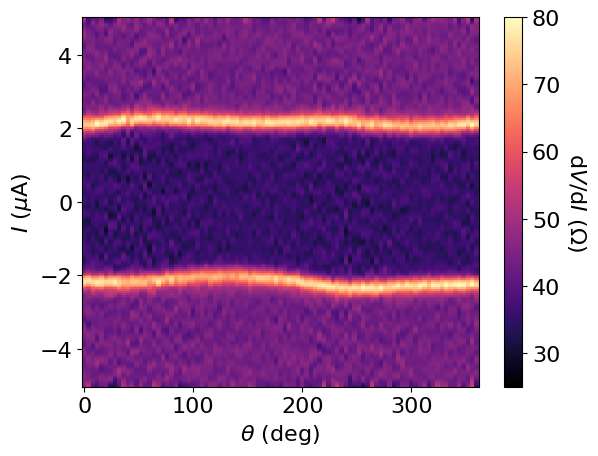
\includegraphics[width=0.32\textwidth]{dVdIthetasweep_72.png}
         %\caption{A portion of the resist is irradiated with an electron beam in as specified pattern.}
         %\label{c}
     \end{subfigure}
        \caption{$\phi$ and $\theta$ sweeps, corresponding to the same device in each case.}
        \label{fig:}
        
\end{figure}


\subsubsection*{D2: AuNb, 50 nm Nb}
\subsubsection*{Z Direction, High Field}


\begin{figure}[H]
     \centering
     \begin{subfigure}[b]{\textwidth}
         \centering
         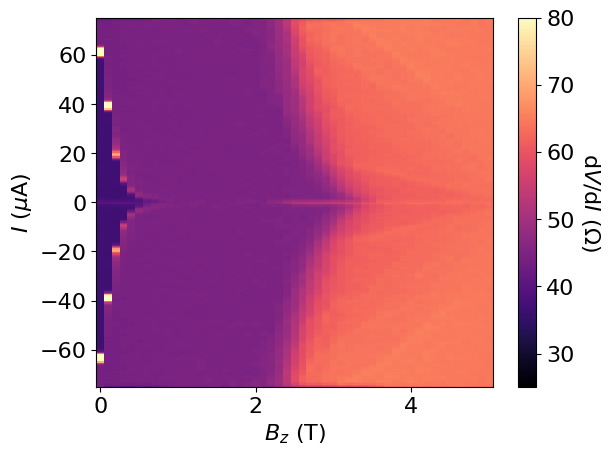
\includegraphics[width=0.32\textwidth]{Appendix_D/D2/dVdIBZ_109.png}
         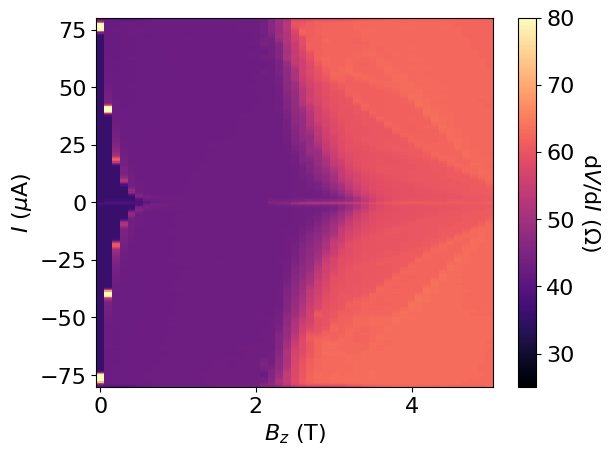
\includegraphics[width=0.32\textwidth]{Appendix_D/D2/dVdIBZ_196.png}
         %\caption{A portion of the resist is irradiated with an electron beam in as specified pattern.}
         %\label{c}
     \end{subfigure}
	 \caption{Out of plane BVI measurements.}
     \label{fig:}
        
\end{figure}

\subsubsection*{X,Y,Z directions, Low field}

\begin{figure}[H]
     \centering
     \begin{subfigure}[b]{\textwidth}
         \centering
         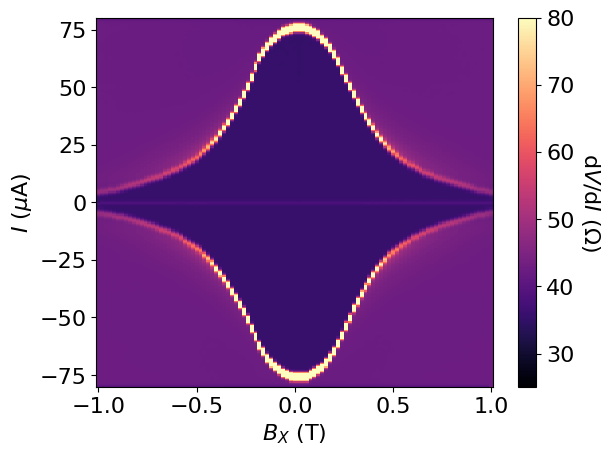
\includegraphics[width=0.32\textwidth]{Appendix_D/D2/dVdIBX_201.png}
         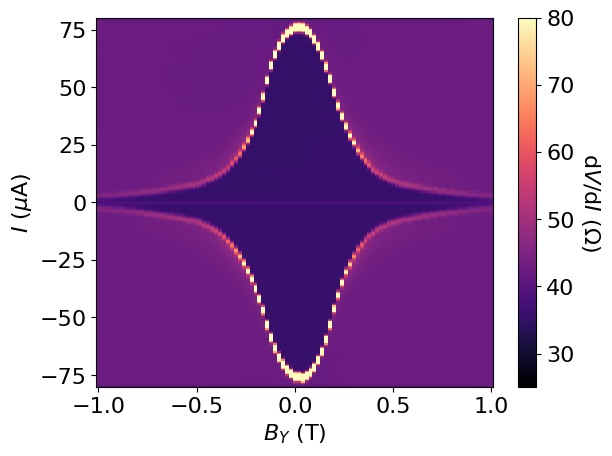
\includegraphics[width=0.32\textwidth]{Appendix_D/D2/dVdIBY_200.png}
         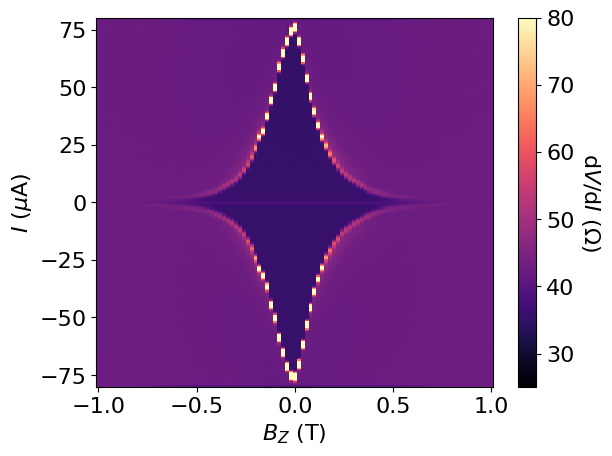
\includegraphics[width=0.32\textwidth]{Appendix_D/D2/dVdIBZ_198.png}
         %\caption{A portion of the resist is irradiated with an electron beam in as specified pattern.}
         %\label{c}
     \end{subfigure}
	 \caption{BVI measurements in the X, Y and Z directions.}
     \label{fig:}
        
\end{figure}

\subsubsection*{$\phi$-Sweep}

\begin{figure}[H]
     \centering
     \begin{subfigure}[b]{\textwidth}
         \centering
         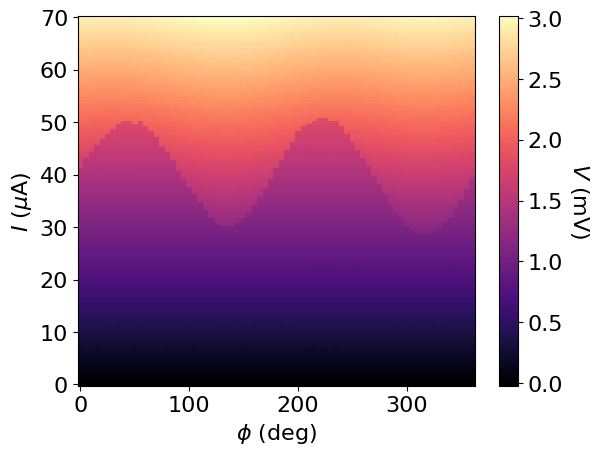
\includegraphics[width=0.32\textwidth]{Appendix_D/D2/phisweep_79.png}
         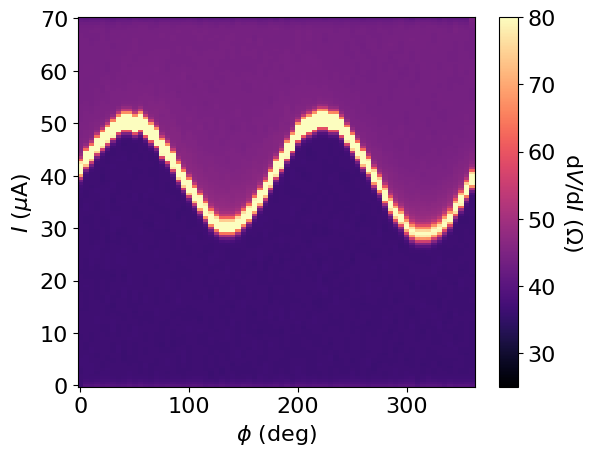
\includegraphics[width=0.32\textwidth]{Appendix_D/D2/dVdIphisweep_79.png}
         %\caption{A portion of the resist is irradiated with an electron beam in as specified pattern.}
         %\label{c}
     \end{subfigure}
     
        \caption{$\phi$ and $\theta$ sweeps, corresponding to the same device.}
        \label{fig:}
        
\end{figure}

\subsubsection*{D3: AuNb, 60 nm Spacing}
\subsubsection*{Z Direction, High Field}



\begin{figure}[H]
     \centering
     \begin{subfigure}[b]{\textwidth}
         \centering
         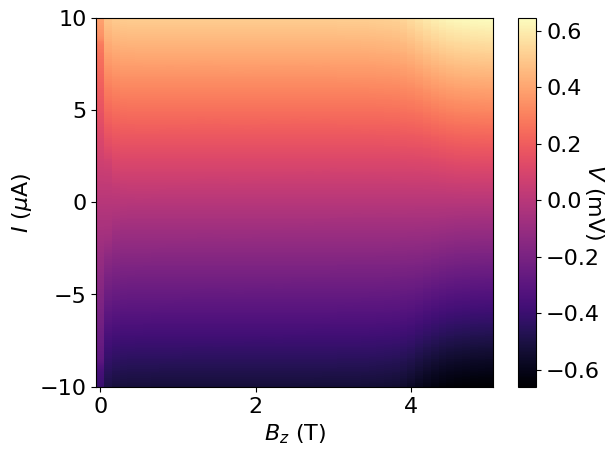
\includegraphics[width=0.32\textwidth]{Appendix_D/D3/VIBZ_17.png}
         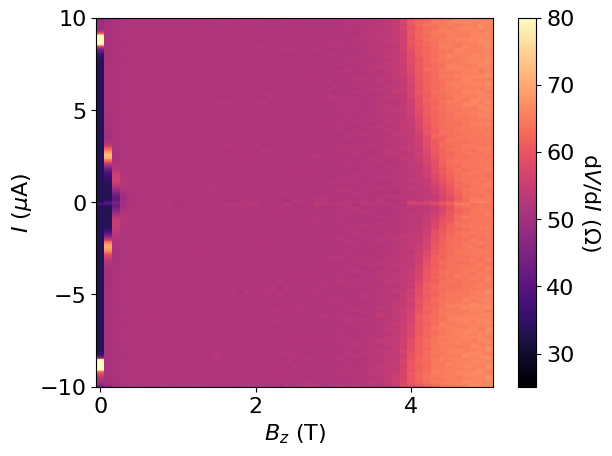
\includegraphics[width=0.32\textwidth]{Appendix_D/D3/dVdIBZ_17.png}
         %\caption{A portion of the resist is irradiated with an electron beam in as specified pattern.}
         %\label{c}
     \end{subfigure}
     
        \caption{Out of plane BVI measurements.}
        \label{fig:}
        
\end{figure}
\subsubsection*{X,Y,Z directions, Low field}

\begin{figure}[H]
     \centering
     \begin{subfigure}[b]{\textwidth}
         \centering
         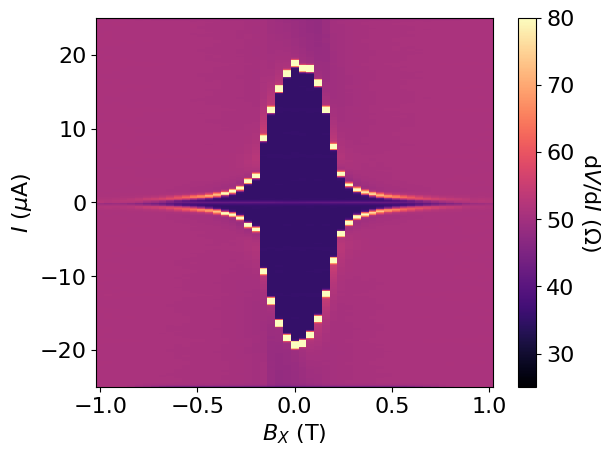
\includegraphics[width=0.32\textwidth]{Appendix_D/D3/dVdIBX_41.png}
         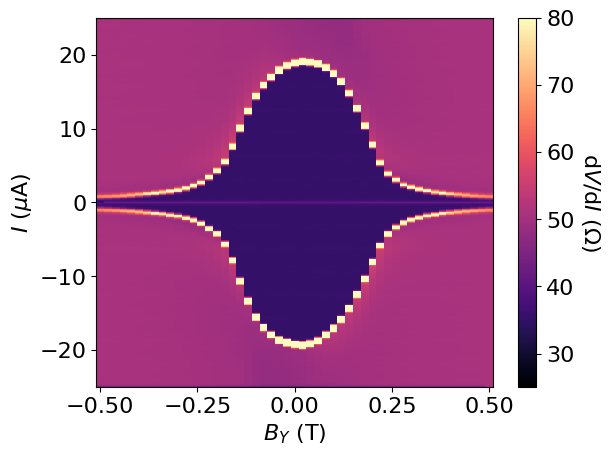
\includegraphics[width=0.32\textwidth]{Appendix_D/D3/dVdIBY_42.png}
         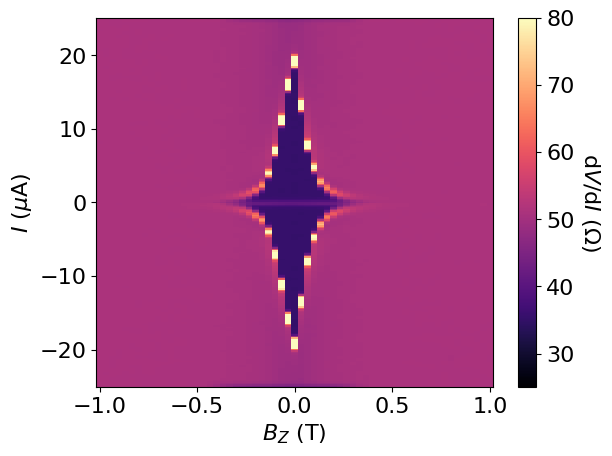
\includegraphics[width=0.32\textwidth]{Appendix_D/D3/dVdIBZ_64.png}
         %\caption{A portion of the resist is irradiated with an electron beam in as specified pattern.}
         %\label{c}
     \end{subfigure}
	 \caption{BVI measurements in the X, Y and Z directions.}
     \label{fig:}
        
\end{figure}

\subsubsection*{$\phi$-Sweep}

\begin{figure}[H]
     \centering
     \begin{subfigure}[b]{\textwidth}
         \centering
         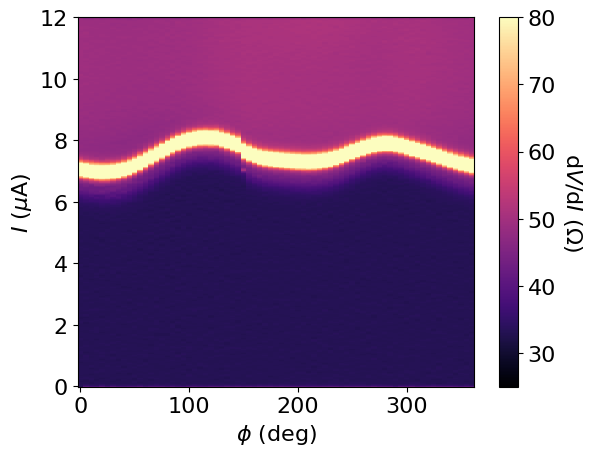
\includegraphics[width=0.32\textwidth]{Appendix_D/D3/dVdIphisweep_22.png}
         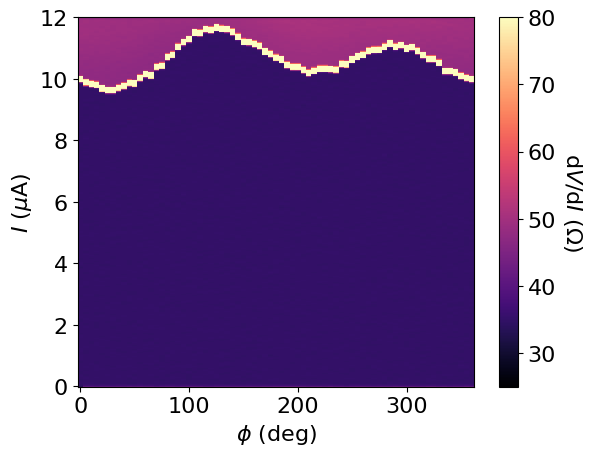
\includegraphics[width=0.32\textwidth]{Appendix_D/D3/dVdIphisweep_23.png}
         %\caption{A portion of the resist is irradiated with an electron beam in as specified pattern.}
         %\label{c}
     \end{subfigure}
	 \caption{$\phi$ and $\theta$ sweeps, corresponding to the same device.}
     \label{fig:}
        
\end{figure}


\subsubsection*{D4: AuNb, 60 nm Spacing}


\subsection{E: Electromigration Curves}
\subsubsection*{E1: PdNb}


\begin{figure}[H]
     \centering
     \begin{subfigure}[b]{\textwidth}
         \centering
         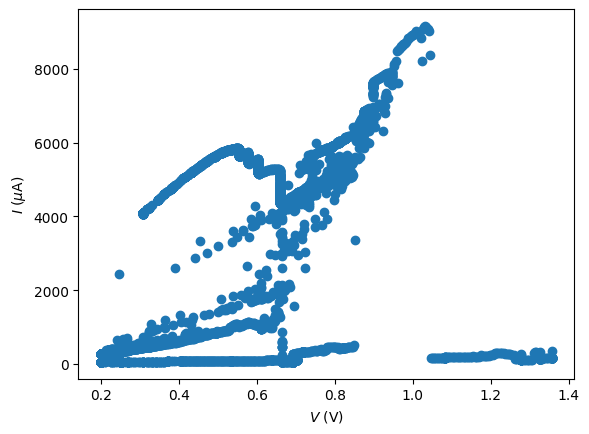
\includegraphics[width=0.32\textwidth]{MigrationIV_A1.png}
         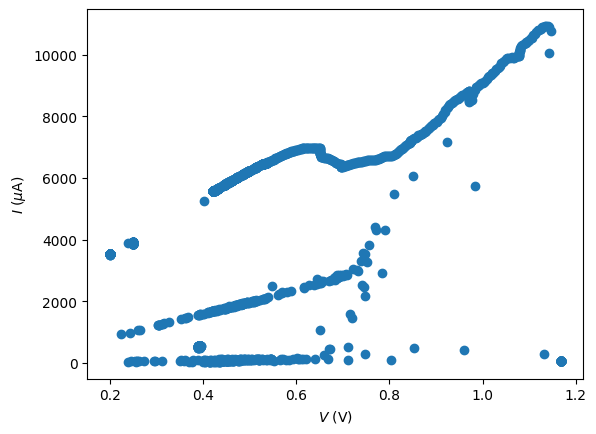
\includegraphics[width=0.32\textwidth]{MigrationIV_B1.png}
         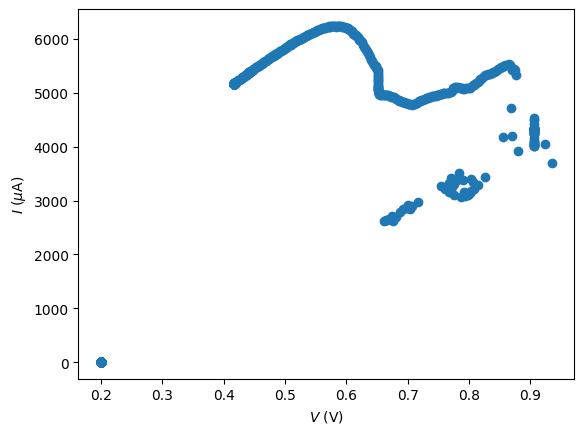
\includegraphics[width=0.32\textwidth]{MigrationIV_B8.png}
         %\caption{A portion of the resist is irradiated with an electron beam in as specified pattern.}
         %\label{c}
     \end{subfigure}
     %\hfill
     \begin{subfigure}[b]{\textwidth}
         \centering
         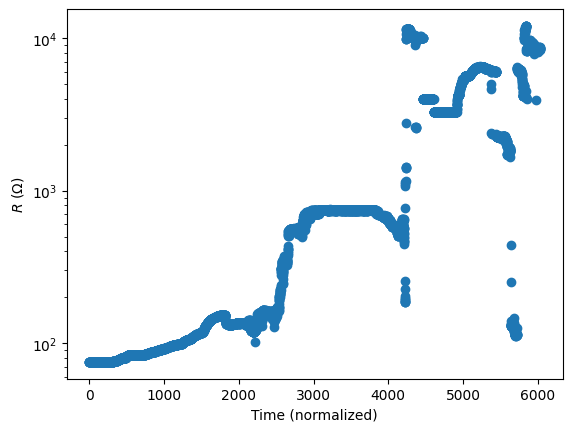
\includegraphics[width=0.32\textwidth]{MigrationRt_A1.png}
         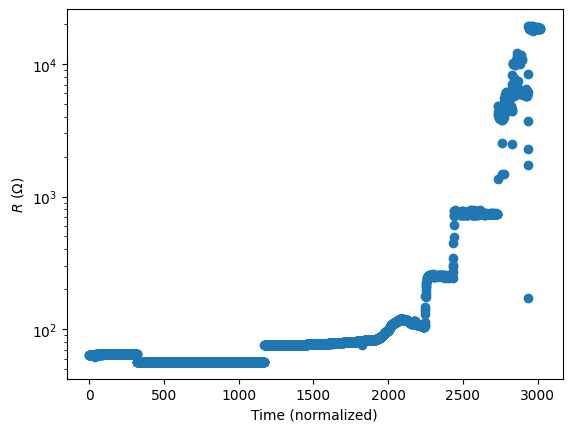
\includegraphics[width=0.32\textwidth]{MigrationRt_B1.png}
         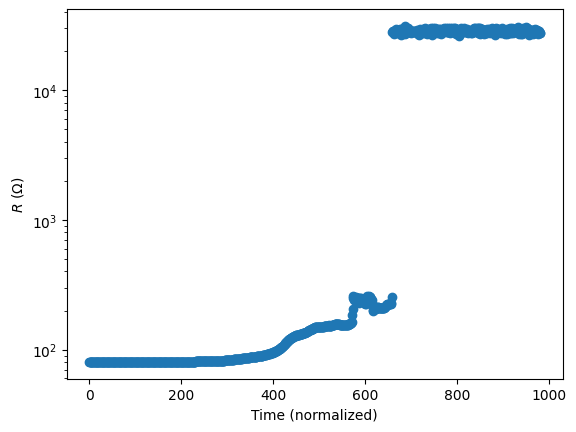
\includegraphics[width=0.32\textwidth]{MigrationRt_B8.png}
         %\caption{A portion of the resist is irradiated with an electron beam in as specified pattern.}
         %\label{c}
     \end{subfigure}
        \caption{Representative electromigration curves.}
        \label{fig:}
        
\end{figure}

\subsubsection*{E2: AuNb, 100 nm Nb}

\begin{figure}[H]
     \centering
     \begin{subfigure}[b]{\textwidth}
         \centering
         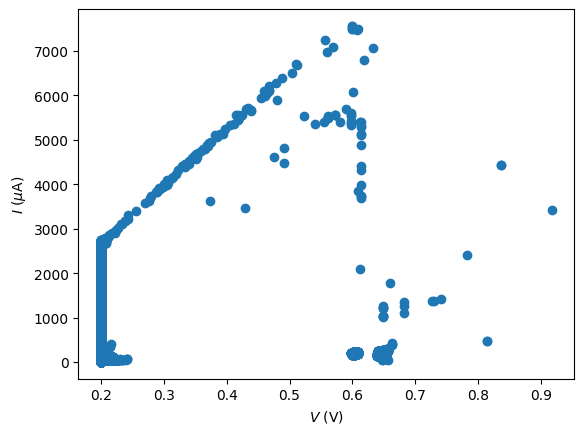
\includegraphics[width=0.32\textwidth]{Appendix_E/E2/MigrationIV_A1.png}
         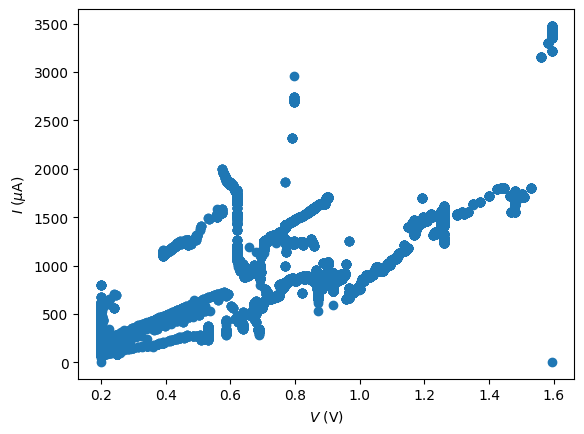
\includegraphics[width=0.32\textwidth]{Appendix_E/E2/MigrationIV_D8.png}
         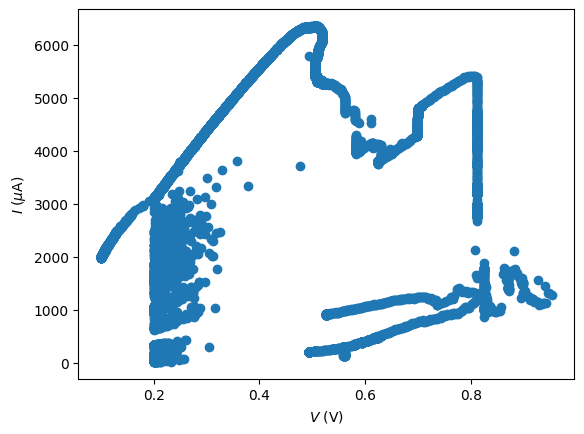
\includegraphics[width=0.32\textwidth]{Appendix_E/E2/MigrationIV_E8.png}
         %\caption{A portion of the resist is irradiated with an electron beam in as specified pattern.}
         %\label{c}
     \end{subfigure}
     %\hfill
     \begin{subfigure}[b]{\textwidth}
         \centering
         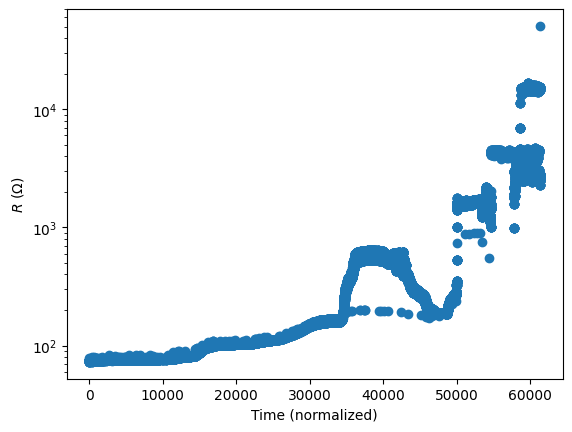
\includegraphics[width=0.32\textwidth]{Appendix_E/E2/MigrationRt_A1.png}
         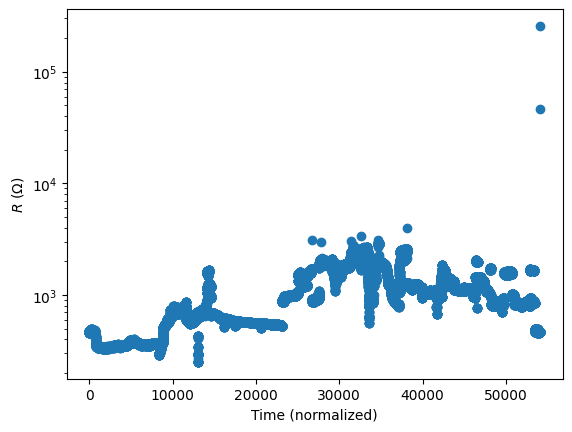
\includegraphics[width=0.32\textwidth]{Appendix_E/E2/MigrationRt_D8.png}
         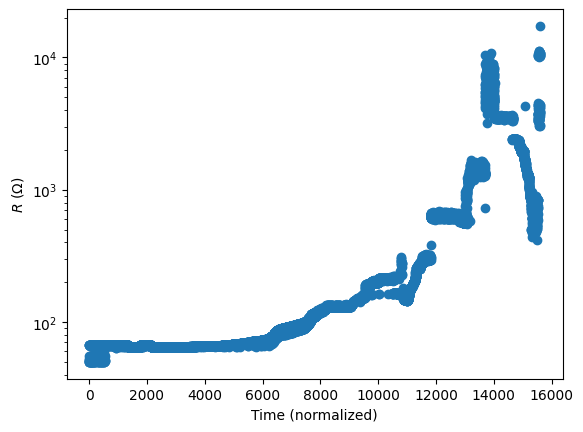
\includegraphics[width=0.32\textwidth]{Appendix_E/E2/MigrationRt_E8.png}
         %\caption{A portion of the resist is irradiated with an electron beam in as specified pattern.}
         %\label{c}
     \end{subfigure}
        \caption{Representative electromigration curves.}
        \label{fig:}
        
\end{figure}

\subsubsection*{E3: AuNb, 50 nm Nb}


\begin{figure}[H]
     \centering
     \begin{subfigure}[b]{\textwidth}
         \centering
         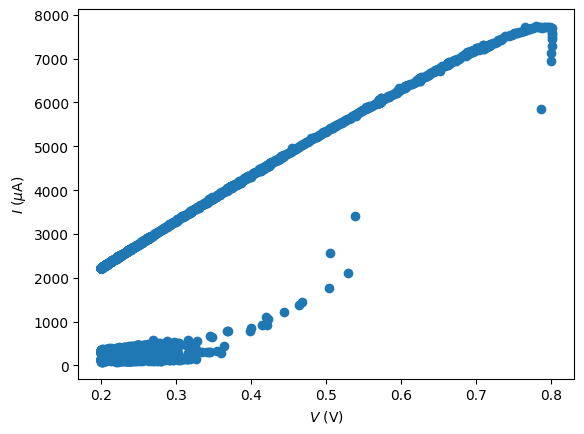
\includegraphics[width=0.32\textwidth]{Appendix_E/E3/MigrationIV_1.png}
         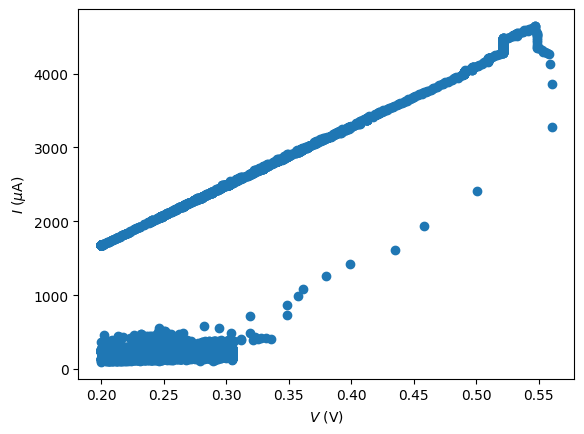
\includegraphics[width=0.32\textwidth]{Appendix_E/E3/MigrationIV_2.png}
         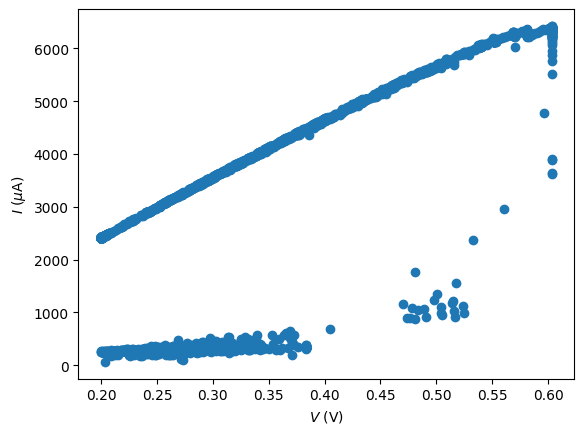
\includegraphics[width=0.32\textwidth]{Appendix_E/E3/MigrationIV_3.png}
         %\caption{A portion of the resist is irradiated with an electron beam in as specified pattern.}
         %\label{c}
     \end{subfigure}
     %\hfill
     \begin{subfigure}[b]{\textwidth}
         \centering
         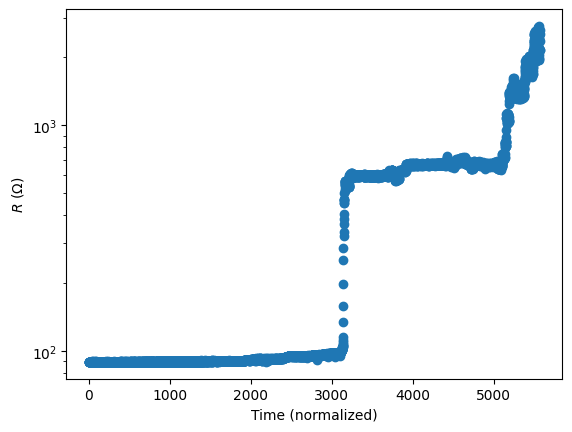
\includegraphics[width=0.32\textwidth]{Appendix_E/E3/MigrationRt_1.png}
         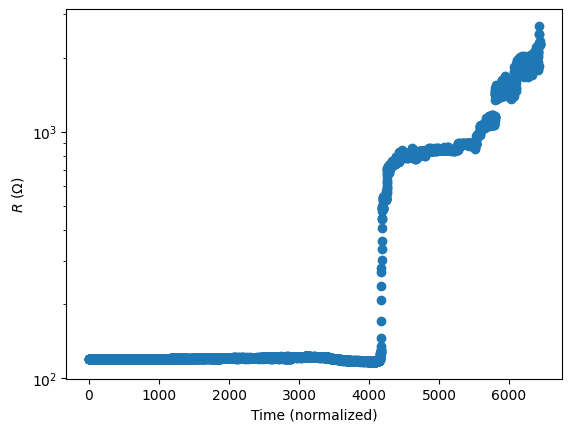
\includegraphics[width=0.32\textwidth]{Appendix_E/E3/MigrationRt_2.png}
         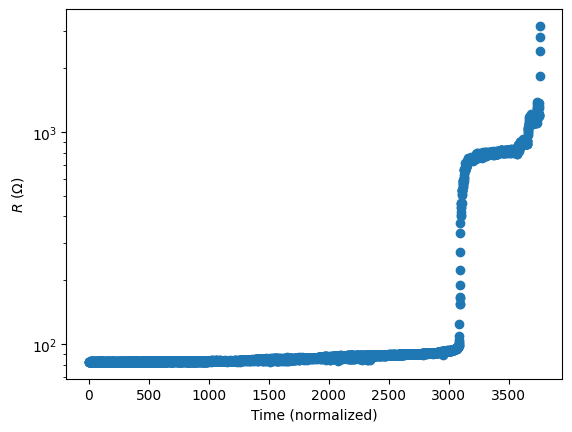
\includegraphics[width=0.32\textwidth]{Appendix_E/E3/MigrationRt_3.png}
         %\caption{A portion of the resist is irradiated with an electron beam in as specified pattern.}
         %\label{c}
     \end{subfigure}
        \caption{Representative electromigration curves.}
        \label{fig:}
        
\end{figure}

\subsubsection*{E4: AuNb, 60 nm Spacing}


\begin{figure}[H]
     \centering
     \begin{subfigure}[b]{\textwidth}
         \centering
         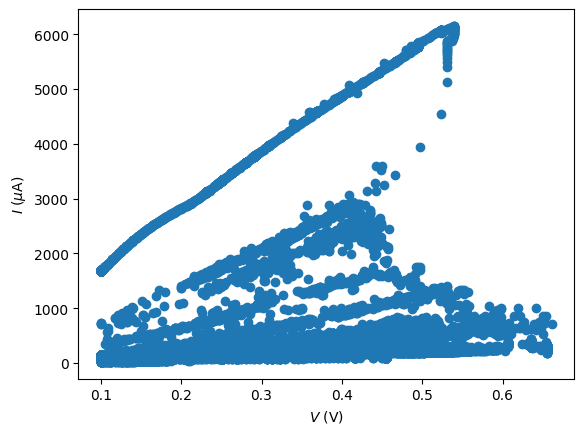
\includegraphics[width=0.32\textwidth]{Appendix_E/E4/MigrationIV_B1.png}
         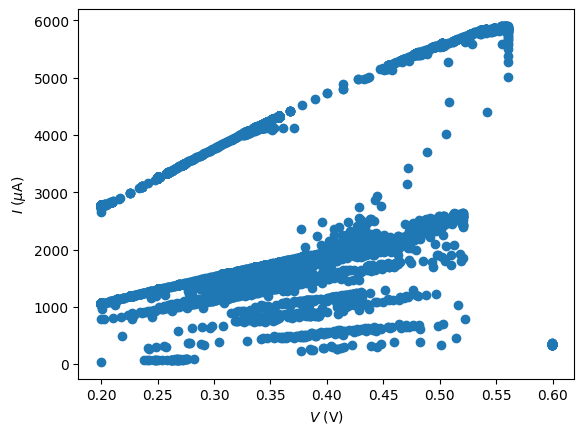
\includegraphics[width=0.32\textwidth]{Appendix_E/E4/MigrationIV_C4.png}
         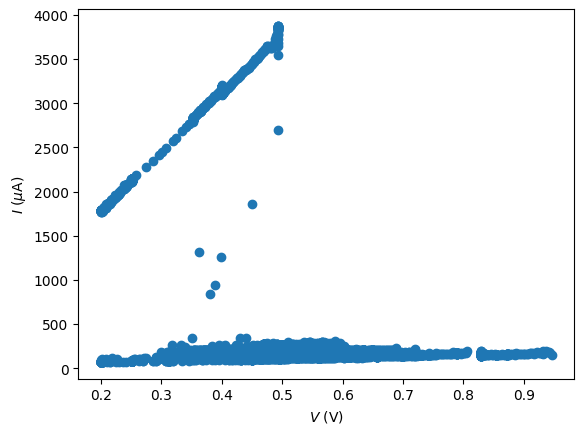
\includegraphics[width=0.32\textwidth]{Appendix_E/E4/MigrationIV_D3.png}
         %\caption{A portion of the resist is irradiated with an electron beam in as specified pattern.}
         %\label{c}
     \end{subfigure}
     %\hfill
     \begin{subfigure}[b]{\textwidth}
         \centering
         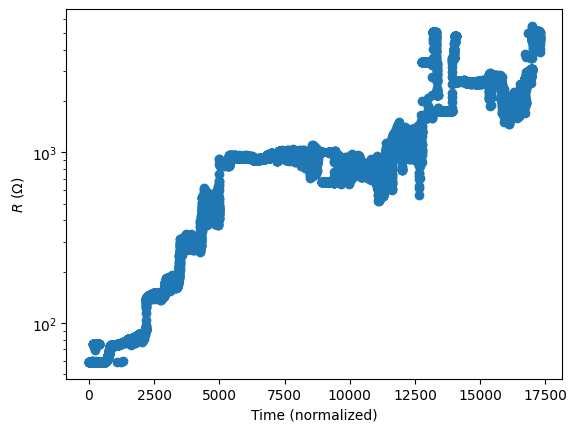
\includegraphics[width=0.32\textwidth]{Appendix_E/E4/MigrationRt_B1.png}
         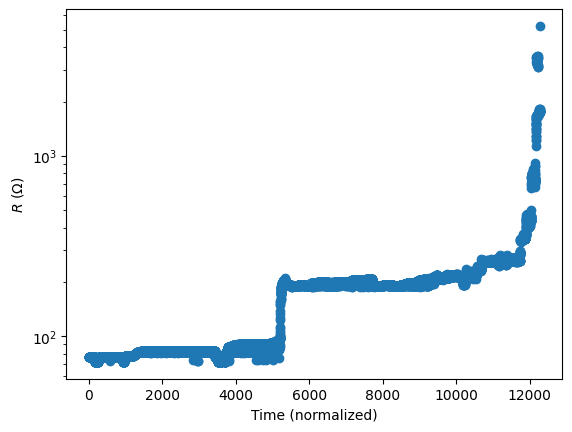
\includegraphics[width=0.32\textwidth]{Appendix_E/E4/MigrationRt_C4.png}
         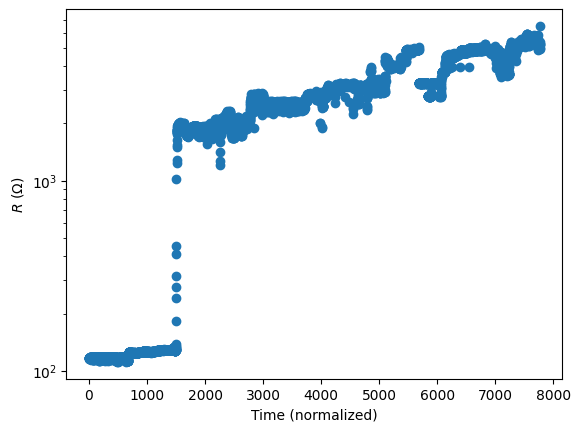
\includegraphics[width=0.32\textwidth]{Appendix_E/E4/MigrationRt_D3.png}
         %\caption{A portion of the resist is irradiated with an electron beam in as specified pattern.}
         %\label{c}
     \end{subfigure}
        \caption{Representative electromigration curves. Since these devices were migrated in stages, the graphs look more chaotic.}
        \label{fig:}
        
\end{figure}





\end{document}